%% The ubcdiss class provides several options:
%%   10pt, 11pt, 12pt
%%       set default font size
%%   oneside, twoside
%%       whether to format for single-sided or double-sided printing
%%   singlespacing, onehalfspacing, doublespacing
%%       set default inter-line text spacing; the ubcdiss class
%%       provides \textspacing to revert to this configured spacing

\documentclass[oneside,onehalfspacing,11pt]{ubcdiss}

% https://tex.stackexchange.com/a/637286/202877
\usepackage[no-math]{fontspec}
\usepackage{mlmodern}
\usepackage[T1]{fontenc}
\usepackage[margin=1.25in, marginparwidth=7em]{geometry}
\usepackage[numbers]{natbib}
\usepackage[hang, sc, skip=1ex]{caption}
\usepackage{marginnote} % margin notes
\usepackage{checkend}	% indicate all unclosed envs
\usepackage{epigraph} % add epigraphs
\usepackage{imakeidx} % add an index
\usepackage{enumitem} % better enumerations and itemizations
\usepackage{graphicx} % graphics and images
\usepackage{multicol} % multiple columns
\usepackage{booktabs} % polished table styling
\usepackage{tikz-cd} % commutative diagrams
\usepackage{xcolor} % coloured text and predefined colours
\usepackage{minted} % code highlighting
\usepackage{amsmath}
\usepackage{amssymb}
\usepackage{amsthm}
\usepackage[pagebackref,bookmarksnumbered,linktocpage,colorlinks]{hyperref}
\usepackage[capitalize, noabbrev]{cleveref} % needs to come after hyperref and amsmath

% backreferences styled as ↪ page(s) x, y, and z
\newcommand{\decline}[3]{\ifcase #1 #3\or #2\else #3\fi}
\renewcommand{\backrefalt}[4]{\textcolor{gray}{$\hookrightarrow$~\decline{#1}{page}{pages}~#2}}

% links must be in "dark blue"
% https://www.grad.ubc.ca/current-students/dissertation-thesis-preparation/fonts-print
\definecolor{darkblue}{HTML}{0000EE}
\hypersetup{allcolors=darkblue}

% use ⬛ as QED symbol
\renewcommand\qedsymbol{$\blacksquare$}

% style URLs (incl. DOIs) in sans serif
\urlstyle{sf}
\newcommand{\doi}[1]{doi:\href{https://doi.org/#1}{\textsf{#1}}}

% epigraph custom styling
\epigraphnoindent
\setlength{\epigraphrule}{0pt}
\newcommand{\epigraphic}[3][0.5]{
  \setlength{\epigraphwidth}{#1\textwidth}
  \epigraph{\textit{#2}}{--- #3}
}

% set caption margins to 2× indent
\setlength{\captionmargin}{2\parindent}

% style margin notes in single-spaced footnotesize Latin Modern
\renewcommand{\marginfont}{\fontfamily{lmr}\selectfont\footnotesize\singlespacing}

% PDF metadata
\hypersetup{
  pdftitle={Sized Dependent Types in Extensional Type Theory},
  pdfauthor={Jonathan Chan},
  pdfsubject={},
  pdfkeywords={},
  pdflang={en-CA}
}

% custom style and macros
\usepackage{style}

\title{Sized Dependent Types in Extensional Type Theory}
\makeindex[intoc]

\author{Jonathan {\footnotesize H.W. \relax}Chan}
\degreetitle{Master of Science}
\institution{The University of British Columbia}
\campus{Vancouver}
\faculty{The Faculty of Graduate and Postdoctoral Studies}
\department{Computer Science}
\submissionmonth{April}
\submissionyear{2022}

\examiningcommittee{William J. Bowman, Assistant Professor, Computer Science}{Supervisor}
%\examiningcommittee{Ronald Garcia, Associate Professor, Computer Science}{Supervisory Committee Member}
%\examiningcommittee{Alexander J. Summers, Associate Professor, Computer Science}{Supervisory Committee Member}

\begin{document}
\maketitle
\makecommitteepage
\textspacing

\chapter{Abstract}

Many contemporary proof assistants based on dependent type theories such as Coq and Agda
are founded on the types-as-propositions paradigm where type checking a program
corresponds to verifying a proof of some proposition in a higher-order predicate logic.
To ensure decidability of type checking and consistency of the logic,
these proof assistants forbid nonterminating recursive functions
using guard predicates that only allow structurally recursive functions
recurring on syntactically smaller arguments.
However, these guard predicates are sometimes too restrictive
and reject simple terminating functions that aren't otherwise structurally recursive.

An alternative is to use type-based termination checking such as sized types,
where inductively-defined types are annotated with sizes.
Successful type checking guarantees that functions recur only on arguments whose types have smaller sizes,
rather than merely on syntactic subarguments.
Some existing models of sized dependent type theories
support features for more expressive sized types,
namely higher-rank size quantification
(which allows for passing around size-preserving functions)
and bounded size quantification
(which eliminates the need for complex semi-continuity checks),
but unfortunately none support both simultaneously.
Meanwhile, the only implementation of sized types in a major proof assistant, Agda,
does support these features, but is unfortunately logically inconsistent.

In this thesis, I design a sized dependent type theory with higher-rank and bounded sizes (\lang),
and show that it's suitable for theorem proving by proving its consistency with a syntactic model:
by compiling \lang into the Extensional Calculus of Inductive Constructions (\CICE),
a variant of Coq's core type theory,
and showing that this translation is type preserving,
the consistency of \lang follows from the consistency of \CICE.

This approach refutes the existence of an ``infinite'' size strictly greater than all sizes,
which is present in prior sized type systems to overcome the limitations of finitary size expressions,
meaning that some infinitary constructs unfortunately aren't definable in \lang.
Even so, \lang provides a valid foundation for sized types in a proof assistant,
opening the way for future work on recovering expressivity lost from the lack of an infinite size
and on restricting sized types in Agda to be consistent.
\chapter{Lay Summary}

While people communicate to one another by speaking or writing in natural languages,
we communicate with computers via programming languages to tell them to, say, perform a calculation.
Just as what's said or written must be grammatically correct to make any sense,
programs written in these programming languages must be checked to ensure that they behave nicely.
One desirable property of programs can be termination:
we want to be certain that they'll eventually finish running at some point.
It's impossible to devise a check that can always pick out all terminating programs,
but approximate termination checks can be improved upon to accept more and more terminating programs.
The topic of this thesis is using \emph{sized types}, a powerful strategy for termination checking,
in the setting of a programming language for mathematicians to write computer-verified proofs,
and proving that the programs that sized typing accepts will actually terminate.
\chapter{Preface}

This thesis is original, independent work by the author, Jonathan Chan.
A summary of the preliminary results of this thesis was presented
as a three-minute recorded lightning talk
at the POPL 2022 Student Research Competition~\citep{SRC}.

\tableofcontents
\listoftables
\listoffigures

\chapter{Acknowledgements}

I'd like to thank the following people for their support throughout the past two years:

\begin{itemize}
  \item William Bowman.
  \item Lily Bryant, for guidance and resources on proving confluence.
  \item Jordy Dickinson, for exposing me to all sorts of niches of type theory and constructive mathematics,
    and for giving an ear to the most out-of-context problems I was working on.
    I hope you're doing well.
  \item Hazel Levine, for making \href{https://types.pl/}{types.pl} a reality (and letting me in on the fun).
  \item The folks on PL Twitter, the TYPES, Coq, Agda, Idris, and Cedille mailing lists and Zulips,
    and the Proof Assistants Stack Exchange for answering my many questions
    and for asking far more interesting ones.
  \item Finally and most importantly, all my other splabmates at the Software Practices Lab
    for making grad school a way better experience than I could have hoped for,
    especially during an ongoing global pandemic.
    To name a few (by increasing order of name length):
    \begin{quote}
    James Yoo\textsuperscript{\href{https://youtu.be/dQw4w9WgXcQ}{0}}, Chris Chen\punctstack{,}\footnote{honourary splabmate}
    Ron Garcia, Adam Geller, Alex Summers, Braxton Hall, Joey Eremondi, Paulette Koronkevich, Felipe Ba\~nados Schwerter,
    \end{quote}
    and many more, especially those who brought treats for the lab.
\end{itemize}

\vfill

This research was supported by the Canada Graduate Scholarships -- Master’s (CGS M) programme.
Cette recherche a \'et\'e financ\'ee par le Programme de bourses d'\'etudes sup\'erieures
du Canada au niveau de la maitrise (BESC M).

\hfill
\chapter{Dedication}

\begin{center}
\textit{Dedicated to the SPL\punctstack{.}}%
\footnote{Special thanks to James Yoo, who took most of these photos.}

\hfill

% TODO: Ask everyone for permission to use
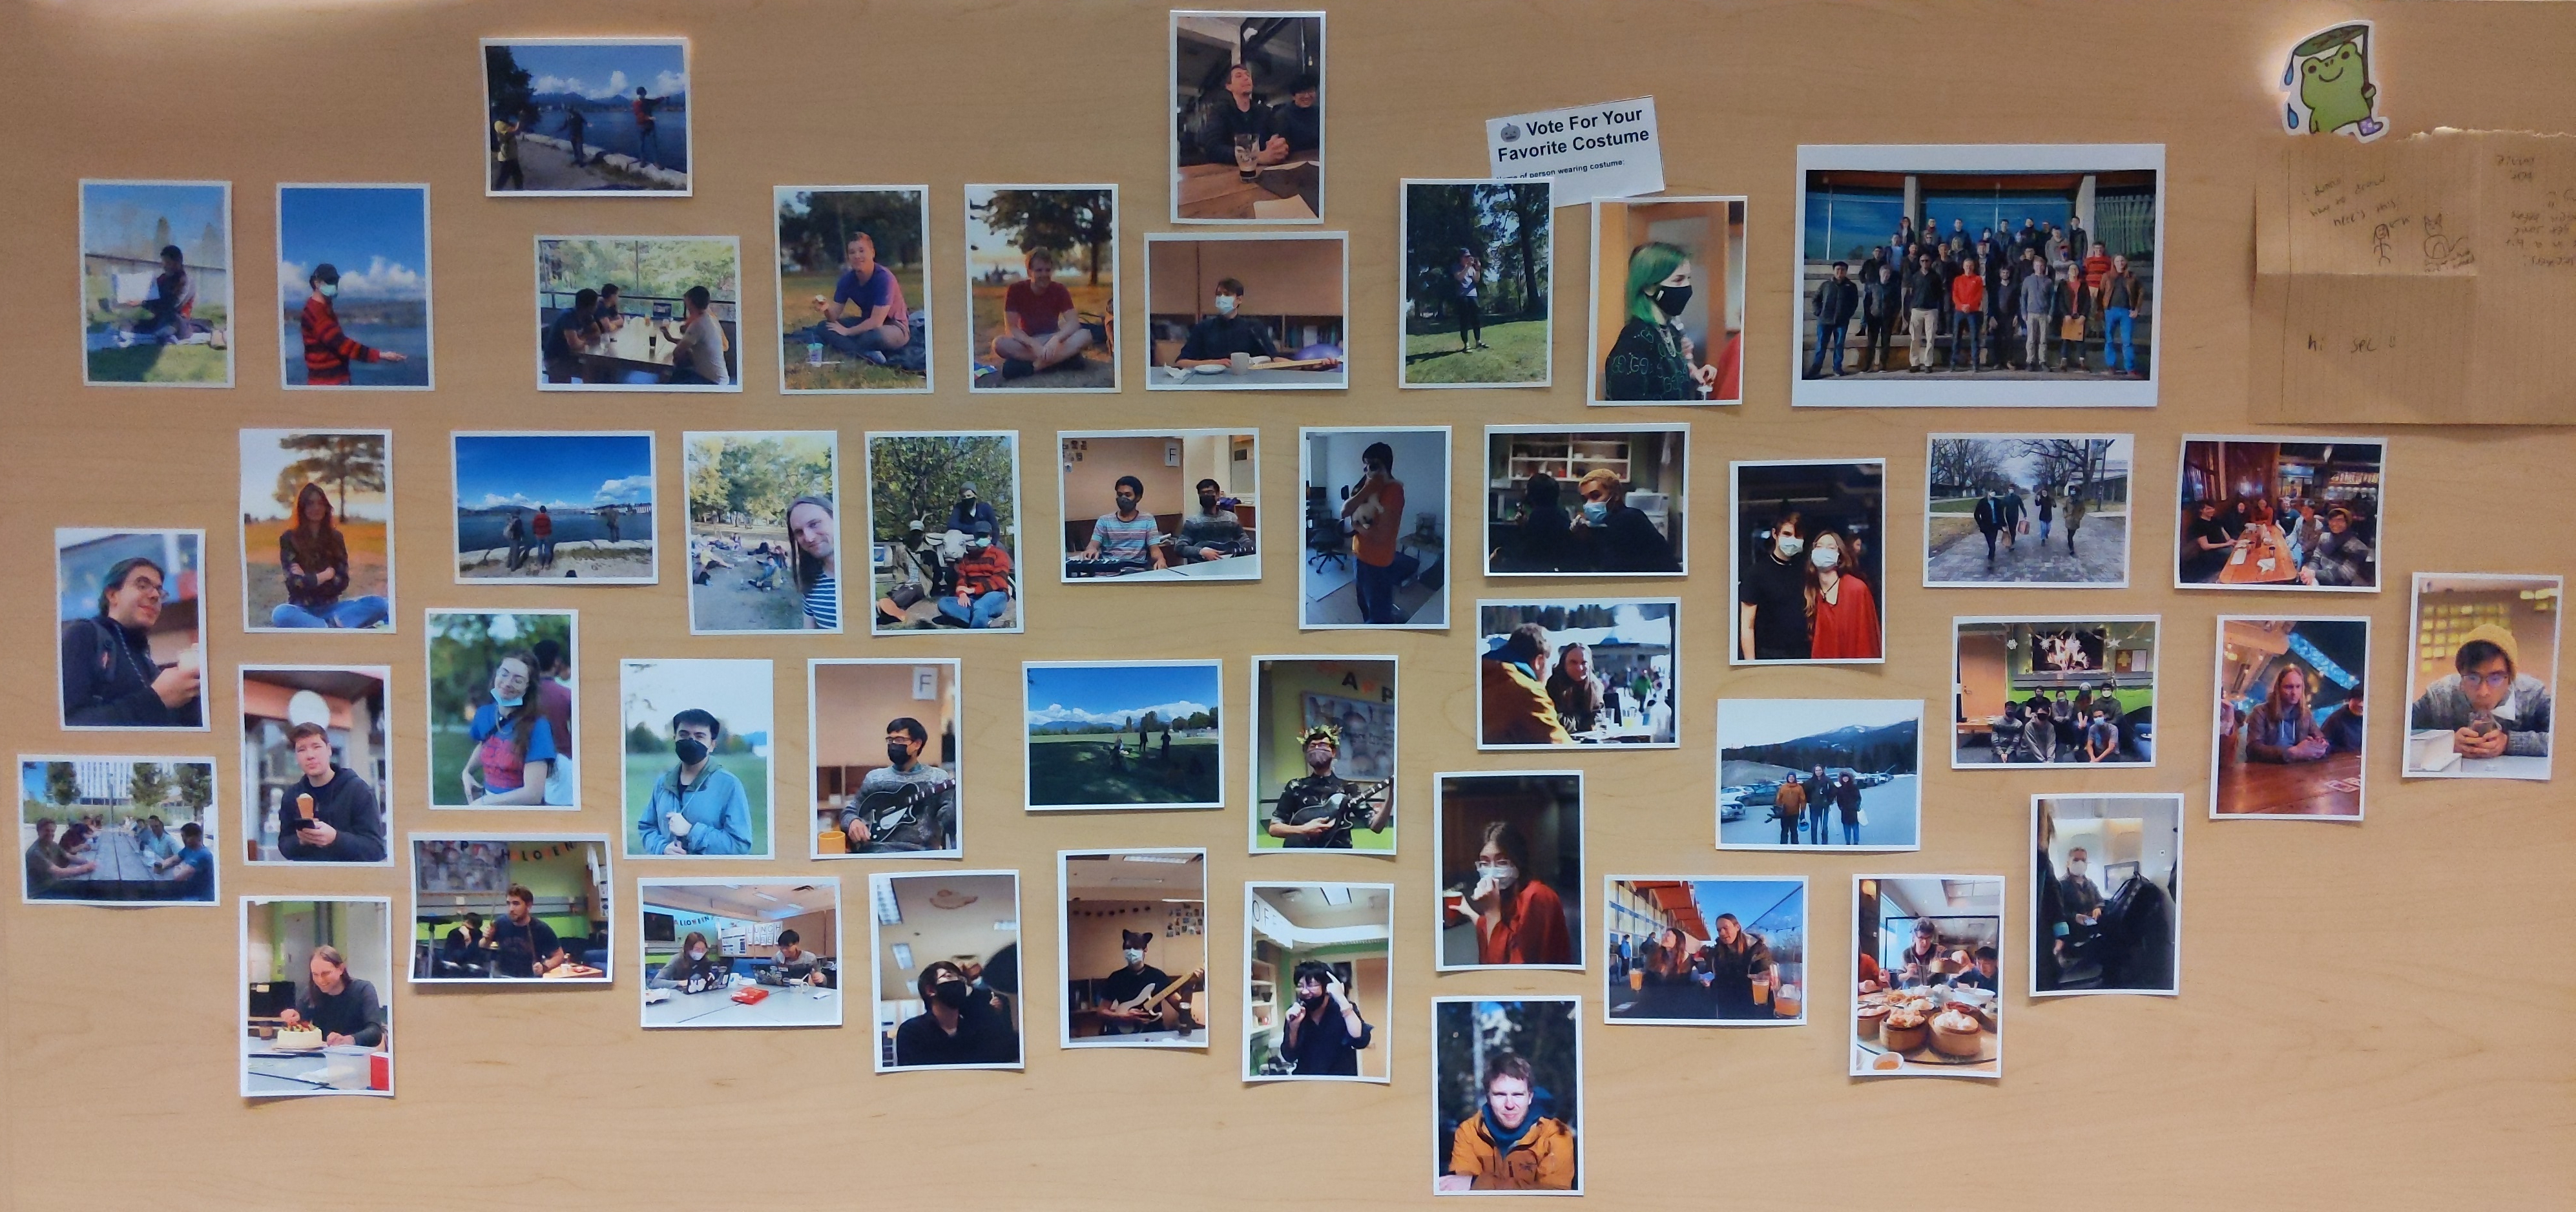
\includegraphics[width=\textwidth]{SPL.jpg}
\end{center}

\mainmatter
\setcounter{chapter}{-1}
\chapter{Typographical Notes}

This thesis is typeset in \href{https://tug.org/FontCatalogue/mlmodern/}{MLModern} by B. Jackowski, J. M. Nowacki, and Daniel Benjamin Miller,
with the exception of the code listings in \cref{app:mechanization},
which are typeset in \href{https://typeof.net/Iosevka/}{\codefont Iosevka} by Belleve Invis (Renzhi Li).

Aside from the standard dark blue links,
the colours in this thesis are selected from a colourblind-friendly palette by \citet{palette}.
Three languages are involved in this thesis:
a metalanguage in \meta{\textbf{bold reddish purple serif}},
a target language in \textcolor{targetcolour}{\texttt{vermillion teletype}},
and a source language in \textit{italic serif} with keywords and names in
\textcolor{kwcolour}{\textsf{orange sans serif}},
\textcolor{constrcolour}{\textsf{bluish green sans serif}},
and \textcolor{constcolour}{\textsf{blue sans serif}}.

Following the \nameref{ch:introduction},
initial appearances of new notation in the text are highlighted in \new{grey}.
\phantom{\citep{phantom}}
\chapter{Introduction} \label{ch:introduction}

A type system is a delicate balance between expressivity and well-behavedness.
More expressivity allows for more programs to be well-typed,
while paradoxically allowing less code to be written,
because some of the onus of ensuring a program is valid is shifted
from the programmer to the process of type checking.
On the other hand, too much expressivity can destroy
desirable metatheoretical properties of the type system ---
strings get be treated as integers, booleans can be called like functions,
and the language falls to chaos and ruin.

The balancing act is particulary perilous for type systems
used by proof assistants for mechanized theorem proving,
because a lack of expressivity can make it too much of a burden to be practically useful,
while it's all to easy to add some convenient, seemingly innocuous feature
that turns out to dismantle the logic of the system,
rendering it unusable for proving.

This thesis deals with dependent type theory, which is commonly used for theorem proving,
together with sized types, a feature for inductively defined types
used to increase the expressivity of recursive functions,
and shows that dependent types can be extended with state-of-the-art sized types
without sacrificing key metatheoretical properties.

\section{Background}

Before we begin, I briefly summarize why dependent types are used for theorem proving,
as well as what sized types have to offer in the context of programming with dependent types.

\subsection{Theorem proving with dependent types} \label{tt}

Many contemporary proof assistants are founded on the Curry--Howard correspondence,
where propositions correspond to types,
proofs of these propositions to terms of those types,
and proof verification to type checking.
Different type theories correspond to different logical systems;
dependent type theories, in particular, correspond to predicate logics.
The primary feature of dependent type theory is the dependent function type,
because it encodes universal quantification by allowing types to \emph{depend on} terms:
the type $\funtype{x}{A}{\app{P}{x}}$ can be interpreted as the statement
``for all objects $x$ in $A$, $P$ holds of $x$'',
with the consequent $\app{P}{x}$ depending on the term $x$.
Other logical constructs can be encoded as well, for example:

\begin{itemize}
  \item Falsehood ($\bot$) as $\funtype{P}{\Prop}{P}$,
    (where $\Prop$ is the type of all propositions),
    the statement that \emph{all} propositions hold;
  \item Implication as $\funtype{\any}{A}{B}$
    (or $\arr*{A}{B}$ for short),
    where $B$ holds only when given a proof of $A$;
  \item Negation as $\arr*{A}{\bot}$,
    or that proving $A$ will yield a falsehood; and
  \item Truthhood as $\funtype{P}{\Prop}{\arr*{P}{P}}$\punctstack{,}%
    \footnote{This encoding is slightly simpler than
    the negation of falsehood $\arr*{\bot}{\bot}$,
    particularly when written out in full.}
    which is trivially inhabited by the identity function
    $\fun{P}{\Prop}{\fun{p}{P}{p}}$;
\end{itemize}
and many other logical connectives such as existential quantification, conjunction, and disjunction.

A key metatheoretical property that a type theory must satisfy
for its interpretation as a logical system to be valid is \emph{consistency}:
falsehood cannot be proven.
In other words, there must not be any term whose type is $\funtype{P}{\Prop}{P}$.
Otherwise, any proposition would be provable,
which goes against the intuition of how a logical system should behave.

The two most important components of a formal description of a dependent type theory
are its typing judgement, whose rules describe when a term has a certain type,
and its equality judgement(s), whose rules describe when two terms are equal.
The latter is relevant in dependent types because they allow determining that,
for instance, a proof of \mbox{$\app{P}{(\app{(\fun{y}{A}{y})}{x})}$}
is in fact also a proof of $\app{P}{x}$.
Naturally, equality is sometimes described in terms of reduction judgements,
governed by the rules of computation.
This means that, in contrast to nondependent type systems,
whether type checking always terminates depends on whether the language is normalizing.
The issue gets even more complicated with more complex forms of reduction like recursion.

\subsection{Recursive programming with sized types} \label{ss}

Inductively defined data and recursive functions on them
are indispensible tools of dependently-typed programming,
allowing the expression of a variety of constructs, programs, and their properties.
A crucial restriction on recursive functions
in proof assistants such as Agda, Coq, Idris, Lean, and more
is that recursive functions must be \emph{guarded by destructors}\index{guardedness}
and only recur on structurally smaller arguments~\citep{guard}.
This guardedness check is statically done before or during type checking and,
to vastly simplify, ensures that recursive calls occur only on syntactic subarguments:
if the original argument is some natural $\app{\succ*}{n}$, then the function recurs only on $n$;
if it's some list $\app{\cons*}{\hd}{\tl}$, then it recurs only on $\tl$;
and so on.

Although this is usually referred to as a syntactic termination check,
and termination is essential in ensuring decidability of type checking,
the key desired property is rather consistency.
Indeed, a type theory may be consistent yet nonnormalizing
(as is the case with an impredicative\index{impredicativity},
definitionally proof-irrelevant $\Prop$ universe~\citep{impred-proof-irrel}),
but unrestricted recursion easily proves an inconsistency:
the recursive function $f$ defined by $\fun{P}{\Prop}{\app{f}{P}}$,
for instance, can be assigned type $\funtype{P}{\Prop}{P}$,
in addition to being nonterminating.

While the guardedness check, being based on the elimination principles of inductive types,
yields terminating functions and a consistent type theory,
it has known disadvantages:

\begin{itemize}
  \item Calling some other function on a subargument prior to a recursive call is disallowed,
    even if that function doesn't change the structure of that subargument,
    because the input of the recursive call is no longer exactly the syntactic subargument.
    For instance, a recursive function on lists cannot first map over the sublist,
    even though the usual mapping function doesn't change the length of a list
    and therefore presents no threat to termination.
  \item Some proof assistants (Coq, for one) will inline functions and even unfold recursive functions
    so that the guardedness check has more information
    and that more recursive functions pass the check.
    However, this too has its disadvantages:
    \begin{itemize}
      \item Programs become nonmodular and noncompositional:
        not only do recursive functions that require inlining
        depend on the implementation of inlined functions,
        they may also depend on their specific implementation details,
        and even a minor syntactic change otherwise equivalent to the original
        can break guardedness~\citep{CIC-hat-minus}.
      \item As aptly summarized by \citet{coqterm},
        \begin{quote}
        \begin{singlespace}
        \textit{{\rm [\ldots]} unfold{\rm [ing]} all the definitions used in the body of the function, do{\rm [ing]} reductions, e.t.c.
        {\rm [\ldots]} makes typechecking extremely slow at times.
        Also, the unfoldings can cause the code to bloat by orders of magnitude and become impossible to debug.}
        \end{singlespace}
        \end{quote}
    \end{itemize}
\end{itemize}

In cases where the guardedness check fails on terminating functions,
the programmer can refactor the function to recur on a different, related argument,
such as the length of a list in the example above,
but this requires additional work and may bloat programs
with extra code solely for satisfying the guardedness check
that detracts from the programs' original intent.
Alternatives to the syntactic guardedness check that avoid these issues are type-based checks,
where the type system itself is augmented so that successful type checking
immediately guarantees termination and consistency.

The one this thesis focuses on is \emph{sized typing}\punctstack{,}%
\footnote{The other common one uses \emph{guarded types}~\citep{guarded-types}.}
where inductive types are annotated with size information,
and constructors construct constructions whose size is larger than that of their subarguments.
In short, the notion of a ``smaller'' subargument is encoded within the types,
no longer requiring syntactic analysis to determine.
Finally, a recursive function is well typed only if it recurs on an argument
whose size is smaller than that of the original argument.

Because well-typedness is the only required condition,
calling some other function before a recursive call is allowed
as long as that function is \emph{size preserving}\index{size preservation}.
For the list mapping example above,
this means that if the sublist of elements of type $\tau$ has size $s$,
then the mapping function must have type $\arr*{\List{\tau}{s}}{\List{\tau}{s}}$.
Notice that the implementation of the mapping function isn't required,
merely its type, thereby avoiding the issues with inlining and unfolding.

This thesis then introduces Sizey \textsc{mc}Type Theory (\lang),
a sized dependent type theory that I prove to be logically consistent consistent
and therefore suitable for both recursive programming and theorem proving.

\section{Overview}

But what need is there for yet another sized type system?
Since \citet{hughes}, there has been a little over two decades' worth of past work on sized types.
\citet{flationary} notes that it has been the topic of at least five dissertations.
This chapter alone names a dozen different type systems with sized types.
There have been many advancements along the way,
but none quite satisfactory to close the matter,
especially when it comes to dependent types.

\lang and this thesis as a whole does not aim to resolve
all of the remaining problems of sized types left open by these past works.
Instead, the purpose is threefold:

\begin{itemize}
  \item To fill an existing gap in sized dependent type theories.
    Two modern sized type features are higher-rank and bounded size quantification,
    and there exist a few dependent type theories with one or the other,
    but not both, to my knowledge.
    On the other hand, they are currently in Agda's implementation of sized types.
    By proving the consistency of \lang, a novel type theory with these two features,
    I bring the theoretical state-of-the-art closer to practice. \\
  \item To demonstrate the viability of using a syntactic model to prove consistency
    of a sized type theory.
    Doing so from scratch through a set-theoretic model is notoriously difficult,
    and often requires sacrifices to and constraints on the type theory;
    see Sacchini's dissertation~\citep{CIC-hat-minus} or \CIChatstar~\citep{CIC-hat-star},
    for instance.
    Instead, a syntactic model relies on the consistency of the language in which I'm modelling,
    and requires no additional deep mathematical knowledge.
  \item To reopen the discussion on sized dependent types.
    Since the discovery of the inconsistency of Agda's sized types~\citep{infinity},
    progress appears to have stagnated a little.
    In later chapters, I examine these difficulties as they might apply to \lang
    and its interpretation in the syntactic model.
\end{itemize}

In this section I describe and justify the design of
the dependent types and the sized types of \lang,
explain how a syntactic model is used to prove its consistency,
and briefly outline the structure of the proof.

\subsection{Dependent types}

As a simple but expressive foundation for dependent types,
I start with the Generalized Calculus of Constructions (\GCC)\index{Calculus of Constructions!Generalized \textasciitilde} \citep{GCC-Coquand},
which has the following features:

\begin{itemize}
  \item \textbf{Dependent function types}, as is standard in the Calculus of Constructions (CC)~\citep{CoC}\index{Calculus of Constructions};
  \item \textbf{Definitions}, \ie locally-named expressions;
  \item \textbf{Universes \ala Russell}\index{universes \ala Russell}, where the types of types are themselves terms
    (as opposed to universes \ala Tarski\index{universes \ala Tarski}, where their \emph{encodings} are terms);
  \item An \textbf{impredicative universe}\index{impredicativity} $\Prop$ such that function types into types in $\Prop$
    are themselves in $\Prop$;
  \item A \textbf{cumulative hierarchy of universes}\index{cumulativity} such that $\Type{i}: \Type{i+1}$,
    any term in $\Type{i}$ is also in $\Type{j}$ given \emph{universe levels}\index{universe level} $i \leq j$,
    and there is a subtyping relation\index{subtyping} on types induced by this inclusion; and
  \item \textbf{Untyped definitional equality} stating when two terms are judgementally equal to one another.
\end{itemize}

These features cover many modern proof assistants.
To name a few, in terms of universes,
Coq and Arend have all of the above;
Lean lacks cumulativity; and
Agda and \Fstar lack cumulativity and an impredicative universe.
On the other hand, these proof assistants all have some form of
\emph{universe level polymorphism},
but this is much more complex and largely orthogonal to sized types
and the syntactic model.

Perhaps the most contentious design decision so far is the use of untyped equality,
as can be found in Coq, over typed equality, as can be found in Agda.%
While typed equality is considered to ``have clearer mathematical semantics''~\citep{typed-NbE},
its judgement depends on the typing judgement;
meanwhile, since types can depend on terms,
typing itself depends on equality to check whether one type can be used in place of another.
As we'll see in \cref{sec:syntactic-model}, these mutually-defined judgements would greatly complicate the proofs,
so I settle for untyped equality instead.

On top of \GCC, I add two inductive definitions featured in Martin--L\"of type theory (MLTT)~\citep{mltt}\index{Martin--L\"of type theory}:
the \emph{Peano naturals} and \emph{well-founded trees}\punctstack{,}%
\footnote{The types of well-founded trees are also known as \emph{W types}.}
augmented with sizes.
As the simplest nontrivial inductive,
the naturals make it easy to demonstrate intuitive uses of sized inductives.
On the other hand, well-founded trees are an example of \emph{generalized} inductives,
with recursive arguments that are functions that return well-founded trees.
They can encode all (nonnested) inductives,
as well as their induction principles \citep{whynotW} if there are dependent pair types
and a \emph{propositional equality}\index{propositional equality} type.
I don't add inductive types in general in their place
because the syntactic baggage that comes with handling the generalization
obscures the intuition behind sized inductive types and the syntactic model,
while it's easy to see how one \emph{could} go from the naturals and well-founded trees
to inductive types in general.

\subsection{Sized types}\label{sec:sized-types}

Sized types are introduced with explicit size quantification $\Funtype{\alpha}{\tau}$,
size abstraction $\Fun{\alpha}{e}$, and size application $\App{e}{s}$.
Sizes themselves consist of size variables as well as a \emph{base size}
and a \emph{size successor operator}.
This is the standard for size expressions in sized type systems.
Some augment the size grammar with addition of or scalar multiplication of size variables,
for instance, increasing expressivity at the expense of complexity.
To keep things simple, I don't include these features and stick to successor sizes.
Note that size expressions here are \emph{not} terms,
and their quantifications, abstractions, and applications
are syntactically distinct from those of terms,
similar to how, in nondependent polymorphic type systems,
types are distinct from terms.

Having explicit sizes differs from some most prior sized type systems where,
extending the type polymorphism analogy,
there is only implicit \emph{rank-1} or
\emph{prenex} size quantification:
size quantifications never appear inside of a type,
and in fact all size abstractions and applications are fully inferred.
Explicit sizes, in contrast, let us express
\emph{higher-rank} size quantification,
which allow for more expressiveness:
for instance, supposing we have cons lists parametrized over some sized type $\tau$,
one could write a size-preserving mapping function over a list
that leaves the sizes untouched.
The type of such a function might be

\vspace{-0.25\baselineskip}
$$\Funtype{\alpha}{\arr*{(\Funtype{\beta}{\arr*{\App{\tau}{\beta}}{\App{\tau}{\beta}}})}{\app{\List*}{(\App{\tau}{\alpha})}}{\app{\List*}{(\App{\tau}{\alpha})}}}.$$

Along with higher-rank sizes, I also include \emph{bounded} size quantification $\Funtype<{\alpha}{s}{\tau}$
and abstraction $\Fun<{\alpha}{s}{e}$.
An order on sizes is induced by these bound instantiations and the successor operator;
this order has nothing to do with subtyping,
and in particular we do \emph{not} have subtyping relations between
$\N{\alpha}$ and $\N{\sss{\alpha}}$, for instance.
Fixpoint expressions recur on smaller sizes according to the order,
summarized by the below typing rule.
%
\begin{mathpar}
\inferrule[]{
  \check{\Phi, \alpha; \Gamma, f: \Funtype<{\beta}{\alpha}{\subst{\tau}{\alpha}{\beta}}}{e}{\tau}
}{
  \infer{\Phi; \Gamma}{\fix{f}{\alpha}{\tau}{e}}{\Funtype{\alpha}{\tau}}
}
\end{mathpar}

Bounded sizes were originally introduced to avoid complex
\emph{semi-continuity} or approximative \emph{polarity}
requirements on fixpoints' types in the presence of an \emph{infinite size}\index{infinite size}
that is strictly larger than all sizes.
Although I don't include an infinite size,
this style of recursion is more elegant because it corresponds neatly to well-founded induction on sizes.

In summary, the sized type features I include are:

\begin{itemize}[noitemsep]
  \item \textbf{Explicit size} quantification $\Funtype{\alpha}{\tau}$,
    abstraction $\Fun{\alpha}{e}$, and
    application $\App{e}{s}$;
  \item A \textbf{simple size grammar} with size variables $\alpha$, a base size $\circ$, and successors $\sss{s}$;
  \item \textbf{Higher-rank sizes}, \eg $\arr*{(\Funtype{\alpha}{\tau})}{\sigma}$;
  \item \textbf{Bounded size} quantification $\Funtype<{\alpha}{s}{\tau}$ and
  abstraction $\Fun<{\alpha}{s}{e}$.
\end{itemize}

Notably, these are all features found in Agda's implementation of sized types.
The only missing feature is the infinite size,
since its properties and its use are known to be inconsistent in Agda.
A demonstration of the inconsistency of a hypothetical infinite size in \lang
is given in \cref{sec:infinity}.

\subsection{Syntactic model}\label{sec:syntactic-model}

To show that \lang is consistent and therefore a suitable type theory for proofs,
I define for it a \emph{syntactic model}\index{syntactic model}~\citep{syntactic-models}.
This involves defining a translation from \lang into some target type theory
in whose consistency we have more confidence---in this case,
the \emph{Extensional Calculus of Inductive Constructions}\index{Calculus of Inductive Constructions!Extensional \textasciitilde}
(\CICE)~\citep{CICE}.
It, too, has a cumulative hierarchy of universes \ala Russell and an impredicative universe,
augmented with inductive types and \emph{equality reflection}\index{equality reflection},
where a definitional equality between terms can be derived from a propositional one between them.
The most notable difference from \lang, aside from these features and sized types,
is that \CICE uses a typed, declarative equality rather than an untyped, algorithmic equality
to better accomodate equality reflection.
For concision and to avoid confusion, I henceforth refer to the former as \emph{equivalence}\index{equivalence},
and to the latter as \emph{conversion}\index{conversion}.

This translation from \lang to \CICE must be \emph{type preserving}\index{type preservation}%
\footnote{This terminology comes from compilation;
in the context of syntactic modelling, this is rather unhelpfully known as \emph{soundness}.}:
if some term $e$ is well typed under some environments $\Phi; \Gamma$ with some type $\tau$,
then the translated term $\compile{e}$ must also be well typed
under the translated environment $\compile{\Phi}\compile{\Gamma}$
with the translated type $\compile{\tau}$.
By the consistency of \CICE and a type-preserving translation to it,
we prove the consistency of \lang.

\begin{postulate}[Consistency of \CICE]\label{fact:consistency-cice}
There exists no term $\eT$ such that
\mbox{$\type{\mt}{\eT}{\funtypeT{\PT}{\PropT}{\PT}}$}.
\end{postulate}

\begin{theorem}[Consistency of \lang]\label{thm:overview:consistency}
Suppose $\compile{\bot} = \funtypeT{\PT}{\PropT}{\PT}$.
Then there exists no term $e$ such that \mbox{$\type{\mt \mathbin{;} \mt}{e}{\bot}$}.
\end{theorem}
\begin{proof}
Suppose that there were such a term $e$.
By the type-preserving translation, we would have that
$\type{\mt}{\compile{e}}{\funtypeT{\PT}{\PropT}{\PT}}$ holds.
However, this contradicts \cref{fact:consistency-cice},
so there must not be such a term.
\end{proof}

What remains, then, is to define $\bot$ and an appropriate translation from \lang to \CICE
such that $\compile{\bot} = \funtypeT{\PT}{\PropT}{\PT}$,
and to show that this translation is type preserving.
I define my translation by induction on the typing derivations of \lang
rather than merely over its syntax,
ensuring that only well-typed terms have a translation.

Type preservation of the translation is proven by induction on not only the typing derivations,
but also the derivations of the judgements on which the typing rules depend.
In particular, typing depends on subtyping\index{subtyping}, which in turn depends
on \emph{$\alpha$-cumulativity}\index{$\alpha$-cumulativity}~\citep{MetaCoq}
and on the reflexive, transitive, congruent closure of reduction.
Finally, this closure of reduction depends on the reduction rules,
most of which are defined by substitution.
Below are the relevant rules showing these dependencies and an example reduction rule.
%
\begin{mathpar}
\inferrule[]{
  \dots \\\\
  \infer{\Phi; \Gamma}{e}{\sigma} \\\\
  \subtype{\Phi; \Gamma}{\sigma}{\tau}
}{
  \check{\Phi; \Gamma}{e}{\tau}
}

\inferrule[]{
  \acum{\sigma_1}{\sigma_2} \\\\
  \red*{\Phi; \Gamma}{\tau_1}{\sigma_1} \\\\
  \red*{\Phi; \Gamma}{\tau_2}{\sigma_2}
}{
  \subtype{\Phi; \Gamma}{\tau_1}{\tau_2}
}

\inferrule[]{
  \red{\Phi; \Gamma}{e_1}{e_2}
}{
  \red*{\Phi; \Gamma}{e_1}{e_2}
}

\inferrule[]{~}{
  \red{\Phi; \Gamma}{\app{(\fun{x}{\tau}{e})}{e'}}{\subst{e}{x}{e'}}
}
\end{mathpar}

We therefore need some lemmas showing that the translation respects
substitution, reduction, the closure of reduction, $\alpha$-cumulativity, and subtyping
in order to prove type preservation.
In short, substitution satisfies a \emph{compositionality}\index{compositionality} principle,
reduction of terms are equivalent by the \CICE equivalence judgement
$\defeq{\GammaT}{\eT_1}{\eT_2}{\tauT}$,
and $\alpha$-cumulative terms and subtypes are correspondingly \CICE subtypes.
I summarize them here, omitting some hypotheses and sublemmas,
to outline the proof architecture,
which roughly follows the structure of type-preserving compilation by~\citet{wjb}.

\begin{lemma}[Compositionality]\label{lem:overview:compositionality}\hfill
\begin{enumerate}[noitemsep]
  \item $\compile{\subst{e}{x}{e'}} = \subst{\compile{e}}{x}{\compile{e'}}$.
  \item $\compile{\subst{e}{\alpha}{s}} = \subst{\compile{e}}{\alpha}{\compile{s}}$
\end{enumerate}
\end{lemma}

\begin{proof}
By induction on the derivation of $\type{\Phi; \Gamma}{e}{\tau}$.
\end{proof}

\begin{lemma}[Preservation of reduction]\label{lem:overview:pres-red}
If $\red{\Phi; \Gamma}{e}{e'}$ and
$\type{\compile{\Phi}\compile{\Gamma}}{\compile{e}}{\tauT}$
then $\defeq{\compile{\Phi}\compile{\Gamma}}{\compile{e}}{\compile{e'}}{\tauT}$.
\end{lemma}

\begin{proof}
By cases on the derivation of $\red{\Phi; \Gamma}{e}{e'}$,
using inversion on the derivation of $\type{\compile{\Phi}\compile{\Gamma}}{\compile{e}}{\compile{\tau}}$,
\cref{lem:overview:compositionality},
and an application of equality reflection in the case for reduction of fixpoints.
\end{proof}

\begin{lemma}[Preservation of reflexive, transitive, congruent closure of reduction]\label{lem:overview:pres-red*}
If $\red*{\Phi; \Gamma}{e}{e'}$ and
$\type{\compile{\Phi}\compile{\Gamma}}{\compile{e}}{\tauT}$
then $\defeq{\compile{\Phi}\compile{\Gamma}}{\compile{e}}{\compile{e'}}{\tauT}$.
\end{lemma}

\begin{proof}
By induction on the derivation of $\red*{\Phi; \Gamma}{e}{e'}$,
using \cref{lem:overview:pres-red},
subject reduction of \lang,
and subject equivalence of \CICE.
\end{proof}

\begin{lemma}[Preservation of $\alpha$-cumulativity]\label{lem:overview:pres-acum}
If $\acum{\tau_1}{\tau_2}$ and
$\type{\compile{\Phi}\compile{\Gamma}}{\compile{\tau_i}}{\UT_i}$
then $\subtype{\compile{\Phi}\compile{\Gamma}}{\compile{\tau_1}}{\compile{\tau_2}}$.
\end{lemma}

\begin{proof}
By induction on the derivation of $\acum{\tau_1}{\tau_2}$,
using inversion on the derivations of $\type{\Phi; \Gamma}{\tau_i}{U_i}$ and
$\type{\compile{\Phi}\compile{\Gamma}}{\compile{\tau_i}}{\UT_i}$.
\end{proof}

\begin{lemma}[Preservation of subtyping]\label{lem:overview:pres-subtyping}
If $\subtype{\Phi; \Gamma}{\tau_1}{\tau_2}$
and $\type{\compile{\Phi}\compile{\Gamma}}{\compile{\tau_i}}{\compile{U}}$
then $\subtype{\compile{\Phi}\compile{\Gamma}}{\compile{\tau_1}}{\compile{\tau_2}}$.
\end{lemma}

\begin{proof}
By cases on the derivation of $\subtype{\Phi; \Gamma}{\tau_1}{\tau_2}$,
using \cref{lem:overview:pres-red*}, \cref{lem:overview:pres-acum},
subject reduction of \lang,
and subject equivalence of \CICE.
\end{proof}

\begin{theorem}[Type preservation]\label{lem:overview:pres-typing}\hfill
\begin{enumerate}[noitemsep]
  \item If $\wf{\Phi}{\Gamma}$ then $\wf{}{\compile{\Phi}\compile{\Gamma}}$.
  \item If $\type{\Phi; \Gamma}{e}{\tau}$ then $\type{\compile{\Phi}\compile{\Gamma}}{\compile{e}}{\compile{\tau}}$.
\end{enumerate}
\end{theorem}

\begin{proof}
By mutual induction on the derivations of $\wf{\Phi}{\Gamma}$ and $\type{\Phi; \Gamma}{e}{\tau}$,
using \cref{lem:overview:pres-subtyping}.
\end{proof}

The most important properties required of \lang are subject reduction\index{subject reduction},
used in \cref{lem:overview:pres-subtyping},
and confluence\index{confluence}, which is used to show that subtyping is transitive,
which in turn is used to prove the inversion principles for the typing judgement.

This proof structure is possible by virtue of the non-mutuality of the judgements of \lang
due to the use of untyped conversion\index{conversion} (and hence untyped reduction).
If it were instead typed, then it would mutually depend on typing and subtyping as well,
and the above lemmas would circularly depend on one another~\citep{wjb}. \\

\section{Related Work}

The history and development of sized types spans over two decades of past work,
and that of dependent types far more than that.
I therefore mention here only past work that are directly relevant
or that I refer to again in later chapters.

\subsection{Dependent type theories}

\GCC\index{Calculus of Constructions!Generalized \textasciitilde}
was originally proposed by \citet{GCC-Coquand},
adding a universe hierarchy to CC\index{Calculus of Constructions} with untyped equality
and using \rref{cum} for cumulativity\index{cumulativity}.
The \emph{Extended Calculus of Constructions}\index{Calculus of Constructions!Extended \textasciitilde}
(ECC) by \citet{ECC} adds a dependent pair type
and uses a subtyping relation instead for cumulativity;
\rref{untyped-subtype-prop, untyped-subtype-pi} are the most notable subtyping rules.

\vspace{-\baselineskip}
\begin{mathpar}
\inferrule[\rlabel*{cum}]{
  \type{\Gamma}{e}{\Type{i}}
}{
  \type{\Gamma}{e}{\Type{i+1}}
}
\and
\inferrule[\rlabel{$\preccurlyeq$-prop}{untyped-subtype-prop}]{~}{
  \subtype{\Gamma}{\Prop}{\Type{i}}
}
\and
\inferrule[\rlabel{$\preccurlyeq$-pi}{untyped-subtype-pi}]{
  \Gamma \vdash \sigma_1 \approx \sigma_2 \\
  \subtype{\Gamma, \annot{x}{\sigma_2}}{\tau_1}{\tau_2}
}{
  \subtype{\Gamma}{\funtype{x}{\sigma_1}{\tau_1}}{\funtype{x}{\sigma_2}{\tau_2}}
}
\end{mathpar}

\citet{universes} introduce ways of adding universe polymorphism to \GCC
as well as to a version of \GCC with definitions.
For the purposes of this thesis, I use \GCC to refer to the type theory
with subtyping and definitions.

The \emph{Calculus of Inductive Constructions}\index{Calculus of Inductive Constructions} (CIC) \citep{CIC}
adds inductive types to CC,
while the \emph{Predicative Calculus of Inductive Constructions}\index{Calculus of Inductive Constructions!Predicative \textasciitilde} (pCIC)
further adds definitions and a cumulative universe hierarchy via subtyping\punctstack{.}%
\footnote{More precisely, pCIC refers to Coq's core CIC with the cumulative universe hierarchy
and without an \emph{impredicative $\Set$} universe from version 8 onwards \citep[Chapter~4]{Coq-manual}.
The Coq Reference Manual from version 8.5 onwards refers to it simply as CIC,
as do many others, \eg \citet{CIC-unifier}.
I prefer to use the specific name pCIC,
since most seem to use CIC to refer to whatever Coq's core calculus happens to be based on at the moment,
which is currently pCuIC.}
\citet{pCIC} give a set-theoretic model for a variant of pCIC with typed equality.
The \emph{Predicative Calculus of Cumulative Inductive Constructions}
\index{Predicative Calculus of Cumulative Inductive Constructions} (pCuIC) \citep{pCuIC}
further extends pCIC with additional cumulativity\index{cumulativity} between inductive types,
also providing a set-theoretic model,
and it serves as the modern core calculus of Coq.
Closely related is the MetaCoq project~\citep{MetaCoq}\index{MetaCoq},
which mechanizes pCuIC and various of its metatheorems within Coq itself,
with additional alternate untyped equality and subtyping judgements,
since Coq's implementation of definitional equality is untyped.

\citet{CCE} adds a propositional equality type with
equality reflection\index{equality reflection} to \GCC with \rref{cum} in \CCE,
although transitivity of definitional equality only holds for well-typed terms,
and gives a syntactic model in an extension of CIC.
Following that, \citet{CICE} improve upon the translation,
using ECC with a propositional equality type, typed equality,
and two extensional axioms,
translating from this type theory with equality reflection (ETT) to one without (ITT).
They implement the translation in Template Coq \citep{TemplateCoq},
extending it to include inductive types.

In contrast to these type systems based on CC,
MLTT\index{Martin--L\"of type theory} is a dependent type theory
with a noncumulative universe hierarchy without $\Prop$,
typed equality, and some basic types: the empty type, the unit type,
dependent pair types, disjoint sum types, and a propositional equality type,
as well as the types of naturals and well-founded trees as mentioned.
They can all be implemented as inductive types in pCIC.

The source language \lang and target language \CICE in this thesis aren't exactly
a single type theory from the literature augmented with sized types.
In short, \lang is based on \GCC but with MetaCoq's alternate subtyping rules
and augmented with naturals and well-founded trees,
while \CICE is based on pCIC with extensionality inspired by ETT.

\subsection{Sized type systems}

Sized dependent type systems date all the way back to \CCR by \citet{CCR},
although its sized types are formulated quite differently from ``modern'' sized types.
The first sized dependent type theory recognized as such is \CIChat by \citet{CIC-hat},
which adds prenex sizes
and a size inference algorithm to CIC.
In the intervening years, several nondependent sized type systems were developed,
notably the ML-like type system by \citet{hughes} (independently of \CCR),
\lambdahat~\citep{lambda-hat, lambda-hat-diss},
\Fhat~\citep{F-hat}, and
\Fhattimes~\citep{F-hat-times},
all of which focus on prenex, fully-inferrable sizes.
\Fhatomega~\citep{Abel-diss}, on the other hand,
has higher-rank, explicitly-quantified sizes.
Other sized type systems and more extensive discussions can be found in dissertations by
\citet{lambda-hat-diss} and \citet{Abel-diss}.

\begin{table}[h]
\centering
\iffalse
\begin{tabular}{l c c c l}
Type system & Explicit sizes? & Higher-rank? & Bounded? & Size algebra \\
\hline
\citet{hughes} & \crossmark & \crossmark & \crossmark & $\sss{s}, s + s, n \times s$ \\
\lambdahat~\citep{lambda-hat, lambda-hat-diss} & \crossmark & \crossmark & \crossmark & $\sss{s}$ \\
\Fhat~\citep{F-hat} & \crossmark & \crossmark & \crossmark & $\sss{s}$ \\
\Fhattimes~\citep{F-hat-times} & \crossmark & \crossmark & \crossmark & $\sss{s}, s + s$ \\
\Fhatomega~\citep{Abel-diss} & \checkmark* & \checkmark* & \crossmark & $\sss{s}$ \\
\Fcopomega~\citep{F-omega-cop} & \checkmark* & \checkmark* & \checkmark* & $\sss{s}$ \\
\end{tabular}
\fi

\begin{tabular}{l c c c c}
Type theory & Explicit sizes? & Higher-rank? & Bounded? & Consistent? \\
\hline
\CIChat~\citep{CIC-hat} & \crossmark & \crossmark & \crossmark & \interromark \\
\CIChatminus~\citep{CIC-hat-minus-nat, CIC-hat-minus} & \crossmark & \crossmark & \crossmark & \checkmark* \\
\CChatomega~\citep{CC-hat-omega} & \crossmark & \crossmark & \crossmark & \checkmark* \\
\CIChatl~\citep{CIC-hat-l} & \crossmark & \crossmark & \crossmark & \checkmark* \\
\CIChatsub~\citep{CIC-hat-sub} & \crossmark & \crossmark & \checkmark* & \checkmark* \\
\CIChatstar~\citep{CIC-hat-star} & \crossmark & \crossmark & \crossmark & \interromark \\
\citet{NbE} & \checkmark* & \checkmark* & \crossmark & \checkmark* \\
MiniAgda~\citep{MiniAgda, flationary} & \checkmark* & \checkmark* & \checkmark* & \crossmark \\
\textbf{\lang} & \checkmark* & \checkmark* & \checkmark* & \checkmark*%
\textsuperscript{\labelcref{foot:CICE-consistency}}
\end{tabular}
\caption{Sized dependent type theories and their properties}
\label{tab:sized-types}
\end{table}

\cref{tab:sized-types} lists the sized dependent type theories that follow \CIChat,
along with the main features I focus on:
explicit, higher-rank, bounded size quantification,
and with whether the type theory has been proven consistent.
The type theory of MiniAgda, on which the sized types implemented in Agda are based,
is the only prior one with all three sized type features,
but is known to be inconsistent~\citep{infinity}.
(Interestingly, \Fcopomega~\citep{F-omega-cop}, which extends System F$_\omega$ with (co)inductive types and sized types,
has all three properties \emph{and} has been proven to be strongly normalizing.)
One of the goals of \lang, as mentioned, is to fill in this gap
with a consistent sized dependent type theory with all of the desired features.
However, it's missing two properties that all of these type theories do have:
inductive types in the ``correct'' universes,
and the existence of an infinite size.

% TODO: fix manual footnote number
\footnotetext[6]{\label{foot:CICE-consistency} Under the postulate that \CICE is consistent.}

\begin{center}
\mbox{* * *}
\end{center}
\vspace*{-0.5\baselineskip}

\noindent In the upcoming \cref{ch:sized-dep-types}, I describe the syntax and judgements of \lang in detail
and provide example programs in \lang that make use of sized types.
Next, in \cref{ch:model} I describe \CICE and define the translation from \lang to \CICE.
Following that, in \cref{ch:proofs} I prove various necessary metatheoretical properties
including confluence and subject reduction,
and elaborate on the proof of type preservation and its associated lemmas.
I conclude in \cref{ch:discussion}, dicussing some of the shortcomings of \lang,
namely the universe levels of the inductive types and the lack of an infinite size,
as well directions for future improvement.
\chapter{Sized Dependent Types} \label{ch:sized-dep-types}

\newcommand{\FigSyntax}[1]{
  \begin{figure}[h]
  \centering
  \begin{align*}
  i, j, k, m, n &\Coloneqq \meta{\textrm{naturals}} &
  \Gamma &\Coloneqq \mt \mid \Gamma, \annot{x}{\tau} \mid \Gamma, \define{x}{\tau}{e} &
  r, s &\Coloneqq \alpha \mid \sss{s} \mid \circ \\
  f, g, x, y, z &\Coloneqq \meta{\textrm{term variables}} &
  \Delta &\Coloneqq \mt \mid \Delta, \annot{x}{\tau} &
  U &\Coloneqq \Prop \mid \Type{i} \\
  \alpha, \beta, \gamma &\Coloneqq \meta{\textrm{size variables}} &
  \Phi &\Coloneqq \mt \mid \Phi, \alpha \mid \Phi, \bound{\alpha}{s} \\
  e, P, \tau, \sigma &\Coloneqq \mathrlap{x \mid U \mid \funtype{x}{\tau}{\tau} \mid \fun{x}{\tau}{e} \mid \app{e}{e} \mid \letin{x}{\tau}{e}{e}} \\
  &\mid \mathrlap{\Funtype{\alpha}{\tau} \mid \Funtype<{\alpha}{s}{\tau} \mid \Fun{\alpha}{e} \mid \Fun<{\alpha}{s}{e} \mid \App{e}{s}}
  %&\mid \Pairtype{\alpha}{\tau} \mid \Pair{s}{e} \mid \unpair{\alpha}{x}{e}{e}
  %&\mid \mathrlap{\eq{e}{\tau}{e} \mid \refl{e} \mid \J{P}{d}{p}}
  \end{align*}
  \caption{Syntax (base \lang)}
  \label{#1}
  \end{figure}
}

\newcommand{\FigRed}[1]{
  \begin{figure}[h]
  \centering
  \begin{mathpar}
  \fbox{$\red{\Phi; \Gamma}{e}{e}$} \qquad
  \fbox{$\red*{\Phi; \Gamma}{e}{e}$} \hfill \\
  \inferrule[]{
    (\define{x}{\tau}{e}) \in \Gamma
  }{
    \red{\Phi; \Gamma}{x}{e}
  }
  \and \inferrule[]{~}{\red{\Phi; \Gamma}{\app{(\fun{x}{\tau}{e})}{e'}}{\subst{e}{x}{e'}}}
  %\and \inferrule[]{~}{\red{\Phi; \Gamma}{\J{}{d}{\refl{}}}{d}}
  \and \inferrule[]{~}{\red{\Phi; \Gamma}{\App{(\Fun{\alpha}{e})}{s}}{\subst{e}{\alpha}{s}}}
  \and \inferrule[]{~}{\red{\Phi; \Gamma}{\App{(\Fun<{\alpha}{r}{e})}{s}}{\subst{e}{\alpha}{s}}}
  \and \inferrule[]{~}{\red{\Phi; \Gamma}{\letin{x}{\tau}{e'}{e}}{\subst{e}{x}{e'}}}
  %\and \inferrule[]{~}{\red{\Phi; \Gamma}{\unpair{\alpha}{x}{\Pair{s}{e'}}{e}}{\subst{e}{\alpha, x}{s, e'}}}
  \\\\
  \inferrule[\rlabel{$\rhd^*$-once}{red*-once}]{
    \red{\Phi; \Gamma}{e_1}{e_2}
  }{
    \red*{\Phi; \Gamma}{e_1}{e_2}
  }
  \and
  \inferrule[\rlabel{$\rhd^*$-refl}{red*-refl}]{~}{\red*{\Phi; \Gamma}{e}{e}}
  \and
  \inferrule[\rlabel{$\rhd^*$-trans}{red*-trans}]{
    \red*{\Phi; \Gamma}{e_1}{e_2} \\
    \red*{\Phi; \Gamma}{e_2}{e_3}
  }{
    \red*{\Phi; \Gamma}{e_1}{e_3}
  }
  \and
  \inferrule[\rlabel{$\rhd^*$-cong}{red*-cong}]{
    \text{For every $1 \leq i \leq n$:} \and
    \red*{\Phi'; \Gamma'}{e_i}{e'_i}
  }{
    \red*{\Phi; \Gamma}{\subst{e}{x_1, \seq, x_n}{e_1, \seq, e_n}}{\subst{e}{x_1, \seq, x_n}{e'_1, \seq, e'_n}}
  }
  \end{mathpar}
  \caption{Reduction rules (base \lang)}
  \label{#1}
  \end{figure}
}

\newcommand{\FigSubtype}[1]{
  \begin{figure}[h]
  \centering
  \begin{mathpar}
  \fbox{$\subtype{\Phi; \Gamma}{\tau}{\tau}$} \qquad
  \fbox{$\acum{e}{e}$} \hfill \\
  \inferrule[\rlabel{$\preccurlyeq$-red}{subtype-red}]{
    \red*{\Phi; \Gamma}{\tau_1}{\sigma_1} \\
    \red*{\Phi; \Gamma}{\tau_2}{\sigma_2} \\
    \acum{\sigma_1}{\sigma_2}
  }{
    \subtype{\Phi; \Gamma}{\tau_1}{\tau_2}
  }
  \and
  \inferrule[\rlabel{$\sqsubseteq$-prop}{acum-prop}]{~}{\acum{\Prop{}}{\Type{i}}}
  \and
  \inferrule[\rlabel{$\sqsubseteq$-type}{acum-type}]{i \leq j}{\acum{\Type{i}}{\Type{j}}}
  \and
  \inferrule[\rlabel{$\sqsubseteq$-refl}{acum-refl}]{
  }{
      \acum{e}{e}
  }
  \and
  \inferrule[\rlabel{$\sqsubseteq$-pi}{acum-pi}]{
    \acum{\tau_1}{\tau_2}
  }{
    \acum{\funtype{x}{\sigma}{\tau_1}}{\funtype{x}{\sigma}{\tau_2}}
  }
  \and
  \inferrule[\rlabel{$\sqsubseteq$-forall}{acum-forall}]{
    \acum{\tau_1}{\tau_2}
  }{
    \acum{\Funtype{\alpha}{\tau_1}}{\Funtype{\alpha}{\tau_2}}
  }
  \and
  \inferrule[\rlabel{$\sqsubseteq$-forall$<$}{acum-forall<}]{
    \acum{\tau_1}{\tau_2}
  }{
    \acum{\Funtype<{\alpha}{s}{\tau_1}}{\Funtype<{\alpha}{s}{\tau_2}}
  }
  \end{mathpar}
  \caption{Subtyping and $\alpha$-cumulativity rules}
  \label{#1}
  \end{figure}
}

\newcommand{\FigSubsize}[1]{
  \begin{figure}[h]
  \centering
  \begin{mathpar}
  \fbox{$\wf{\Phi}{s}$} \qquad
  \fbox{$\subsize{\Phi}{s}{s}$} \hfill \\
  \inferrule[]{
    \wf{}{\Phi} \\
    \alpha \in \Phi
    \textit{ or }
    (\bound{\alpha}{s}) \in \Phi
  }{
    \wf{\Phi}{\alpha}
  }
  \and
  \inferrule[]{\wf{}{\Phi}}{\wf{\Phi}{\circ}}
  \and
  \inferrule[]{
    \wf{\Phi}{s}
  }{
    \wf{\Phi}{\sss{s}}
  }
  \and
  \inferrule[]{
    \wf{}{\Phi} \\
    (\bound{\alpha}{s}) \in \Phi
  }{
    \subsize{\Phi}{\sss{\alpha}}{s}
  }
  \\
  \inferrule[]{
    \wf{\Phi}{s}
  }{
    \subsize{\Phi}{\circ}{s}
  }
  \and
  \inferrule[]{
    \wf{\Phi}{s}
  }{
    \subsize{\Phi}{s}{s}
  }
  \and
  \inferrule[]{
    \wf{\Phi}{s}
  }{
    \subsize{\Phi}{s}{\sss{s}}
  }
  \and
  \inferrule[]{
    \subsize{\Phi}{r}{s}
  }{
    \subsize{\Phi}{\sss{r}}{\sss{s}}
  }
  \and
  \inferrule[]{
    \subsize{\Phi}{s_1}{s_2} \\\\
    \subsize{\Phi}{s_2}{s_3}
  }{
    \subsize{\Phi}{s_1}{s_3}
  }
  % \and \inferrule[]{~}{\subsize{\Gamma}{s}{\infty}}
  \end{mathpar}
  \caption{Size and subsizing rules}
  \label{#1}
  \end{figure}
}

\newcommand{\FigWF}[1]{
  \begin{figure}[h]
  \centering
  \begin{mathpar}
  \fbox{$\wf{}{\Phi}$} \qquad
  \fbox{$\wf{\Phi}{\Gamma}$} \hfill \\
  \inferrule[\rlabel{nil}{nil}]{~}{\wf{}{\mt}}
  \and
  \inferrule[\rlabel{cons-size}{cons-size}]{
    \wf{}{\Phi}
  }{
    \wf{}{\Phi, \alpha}
  }
  \and
  \inferrule[\rlabel{cons-size$<$}{cons-size<}]{
    \wf{}{\Phi} \\\\
    \wf{\Phi}{s}
  }{
    \wf{}{\Phi, \bound{\alpha}{s}}
  }
  \and
  \inferrule[nil]{\wf{}{\Phi}}{\wf{\Phi}{\mt}}
  \and
  \inferrule[\rlabel{cons-ass}{cons-ass}]{
    \wf{\Phi}{\Gamma} \\\\
    \infer{\Phi; \Gamma}{\tau}{U}
  }{
    \wf{\Phi}{\Gamma, \annot{x}{\tau}}
  }
  \and
  \inferrule[\rlabel{cons-def}{cons-def}]{
    \wf{\Phi}{\Gamma} \\\\
    \infer{\Phi; \Gamma}{e}{\tau}
  }{
    \wf{\Phi}{\Gamma, \define{x}{\tau}{e}}
  }
  \end{mathpar}
  \caption{Well-formedness rules}
  \label{#1}
  \end{figure}
}

\newcommand{\FigRulesAxioms}[1]{
  \begin{figure}[h]
  \centering
  \begin{align*}
  \axioms{\Prop} &= \Type{1} &
  \rules{U}{\Prop} &= \Prop \\
  \axioms{\Type{i}} &= \Type{i+1} &
  \rules{\Prop}{U} &= U \\
  && \rules{\Type{i}}{\Type{j}} &= \Type{\maximum{i, j}}
  \end{align*}
  \caption{Some metafunctions}
  \label{#1}
  \end{figure}
}

\newcommand{\FigTyping}[1]{
  \begin{figure}[p]
  \centering
  \begin{mathpar}
  \fbox{$\type{\Phi; \Gamma}{e}{\tau}$} \hfill \\
  \inferrule[\rlabel*{conv}]{
    \infer{\Phi; \Gamma}{e}{\sigma} \\
    \check{\Phi; \Gamma}{\sigma}{U} \\\\
    \infer{\Phi; \Gamma}{\tau}{U} \\
    \subtype{\Phi; \Gamma}{\sigma}{\tau}
  }{
    \check{\Phi; \Gamma}{e}{\tau}
  }
  \and
  \inferrule[\rlabel*{var}]{
    \wf{\Phi}{\Gamma} \\
    (\annot{x}{\tau}) \in \Gamma \\\\
    \textit{or } (\define{x}{\tau}{e}) \in \Gamma
  }{
    \infer{\Phi; \Gamma}{x}{\tau}
  }
  \and
  \inferrule[\rlabel*{univ}]{
    \wf{\Phi}{\Gamma} \\
  }{
    \infer{\Phi; \Gamma}{U}{\axioms{U}}
  }
  \and
  \inferrule[\rlabel*{pi}]{
    \infer{\Phi; \Gamma}{\sigma}{U_1} \\
    \infer{\Phi; \Gamma, \annot{x}{\sigma}}{\tau}{U_2}
  }{
    \infer{\Gamma}{\funtype{x}{\sigma}{\tau}}{\rules{U_1}{U_2}}
  }
  \and
  \inferrule[\rlabel*{lam}]{
    \infer{\Phi; \Gamma}{\sigma}{U} \\
    \infer{\Phi; \Gamma, \annot{x}{\sigma}}{e}{\tau}
  }{
    \infer{\Phi; \Gamma}{\fun{x}{\sigma}{e}}{\funtype{x}{\sigma}{\tau}}
  }
  \and
  \inferrule[\rlabel*{app}]{
    \infer{\Phi; \Gamma}{e_1}{\funtype{x}{\sigma}{\tau}} \\
    \check{\Phi; \Gamma}{e_2}{\sigma}
  }{
    \infer{\Phi; \Gamma}{\app{e_1}{e_2}}{\subst{\tau}{x}{e_2}}
  }
  \and
  \inferrule[\rlabel*{let}]{
    \infer{\Phi; \Gamma}{\sigma}{U} \\
    \check{\Phi; \Gamma}{e_1}{\sigma} \\\\
    \infer{\Phi; \Gamma, \define{x}{\sigma}{e_1}}{e_2}{\tau}
  }{
    \infer{\Phi; \Gamma}{\letin{x}{\sigma}{e_1}{e_2}}{\subst{\tau}{x}{e_1}}
  }
  \and
  \inferrule[\rlabel*{forall}]{
    \infer{\Phi, \alpha; \Gamma}{\tau}{U}
  }{
    \infer{\Phi; \Gamma}{\Funtype{\alpha}{\tau}}{U}
  }
  \and
  \inferrule[\rlabel*{slam}]{
    \infer{\Phi,\alpha; \Gamma}{e}{\tau}
  }{
    \infer{\Phi; \Gamma}{\Fun{\alpha}{e}}{\Funtype{\alpha}{\tau}}
  }
  \and
  \inferrule[\rlabel*{sapp}]{
    \infer{\Phi; \Gamma}{e}{\Funtype{\alpha}{\tau}} \\
    \wf{\Phi}{s}
  }{
    \infer{\Phi; \Gamma}{\App{e}{s}}{\subst{\tau}{\alpha}{s}}
  }
  \and
  \inferrule[\rlabel{forall$<$}{forall<}]{
    \wf{\Phi}{s} \\
    \infer{\Phi, \bound{\alpha}{s}; \Gamma}{\tau}{U}
  }{
    \infer{\Phi; \Gamma}{\Funtype<{\alpha}{s}{\tau}}{U}
  }
  \and
  \inferrule[\rlabel{slam$<$}{slam<}]{
    \wf{\Phi}{s} \\
    \infer{\Phi, \bound{\alpha}{s}; \Gamma}{e}{\tau}
  }{
    \infer{\Phi; \Gamma}{\Fun<{\alpha}{s}{e}}{\Funtype<{\alpha}{s}{\tau}}
  }
  \and
  \inferrule[\rlabel{sapp$<$}{sapp<}]{
    \infer{\Phi; \Gamma}{e}{\Funtype<{\alpha}{r}{\tau}} \\
    \subsize{\Phi}{\hat{s}}{r}
  }{
    \infer{\Phi; \Gamma}{\App{e}{s}}{\subst{\tau}{\alpha}{s}}
  }
  \iffalse
  \and
  \inferrule[\rlabel*{exists}]{
    \infer{\Phi, \alpha; \Gamma}{\tau}{U}
  }{
    \infer{\Phi; \Gamma}{\Pairtype{\alpha}{\tau}}{U}
  }
  \and
  \inferrule[\rlabel*{pair}]{
    \wf{\Phi}{s} \\
    \check{\Phi; \Gamma}{e}{\subst{\tau}{\alpha}{s}}
  }{
    \infer{\Phi; \Gamma}{\Pair{s}{e}_{\Pairtype{\alpha}{\tau}}}{\Pairtype{\alpha}{\tau}}
  }
  \and
  \inferrule[\rlabel*{unpair}]{
    \infer{\Phi; \Gamma}{e_1}{\Pairtype{\alpha}{\sigma}} \\
    \infer{\Phi, \alpha; \Gamma, \annot{x}{\sigma}}{e_2}{\tau}
  }{
    \infer{\Phi; \Gamma}{\unpair{\alpha}{x}{e_1}{e_2}}{\tau}
  }
  \and
  \inferrule[\rlabel*{eq}]{
    \infer{\Phi; \Gamma}{\tau}{U} \\
    \check{\Phi; \Gamma}{e_1}{\tau} \\
    \check{\Phi; \Gamma}{e_2}{\tau}
  }{
    \infer{\Phi; \Gamma}{\eq{e_1}{\tau}{e_2}}{U}
  }
  \and
  \inferrule[\rlabel*{refl}]{
    \infer{\Phi; \Gamma}{e}{\tau}
  }{
    \infer{\Phi; \Gamma}{\refl{e}}{\eq{e}{\tau}{e}}
  }
  \and
  \inferrule[\rlabel*{J}]{
    \infer{\Phi; \Gamma}{p}{\eq{e_1}{\tau}{e_2}} \\
    \fresh{y, z} \\\\
    \infer{\Phi; \Gamma, \annot{y}{\tau}, \annot{z}{\eq{e_1}{\tau}{y}}}{\app{\app{P}{y}}{z}}{U} \\
    \check{\Phi; \Gamma}{d}{\app{\app{P}{e_1}}{\refl{e_1}}} \\
  }{
    \infer{\Phi; \Gamma}{\J{P}{d}{p}}{\app{\app{P}{e_2}}{p}}
  }
  \fi
  \end{mathpar}
  \caption{Typing rules}
  \label{#1}
  \end{figure}
}
\newcommand{\FigSyntaxInd}[1]{
  \begin{figure}[h]
  \centering
  \begin{align*}
  c &\Coloneqq \zero* \mid \succ* \mid \sup* &&&&& \\
  %t &\Coloneqq e \mid \mathopen{[} s \mathclose{]} &
  %\Theta &\Coloneqq \mt \mid \Theta, \annot{x}{\tau} \mid \Theta, \alpha \mid \Theta, \bound{\alpha}{s} & \\
  e &\Coloneqq \mathrlap{\cdots \mid \N{s} \mid \zero{s}{s} \mid \succ{s}{s}{e} \mid \W{x}{\tau}{\tau}{s} \mid \sup{x}{\tau}{\tau}{s}{s}{e}{e}} \\
  &\mid \mathrlap{\match{e}{\fun*{x}{P}}{(\app{\App{c}{\alpha}}{z_1 \seq z_m} \Rightarrow e) \seq} \mid \fix{}{f}{\alpha}{\tau}{e}}
\end{align*}
  \caption{Syntax (naturals and well-founded trees)}
  \label{#1}
  \end{figure}
}

\newcommand{\FigRedInd}[1]{
  \begin{figure}[h]
  \centering
  \begin{mathpar}
  \vspace{-2ex}
  \fbox{$\red{\Phi; \Gamma}{e}{e}$} \quad \cdots \hfill \\
  \inferrule[]{~}{
    \red[]{\Phi; \Gamma}{\match*{\App{\zero*_{\any}}{s}}{(\App{\zero*}{\alpha} \Rightarrow e_z) (\app{\App{\succ*}{\any}}{\any} \Rightarrow \any)}}{\subst{e_z}{\alpha}{s}}
  }
  \and
  \inferrule[]{~}{
    \red[]{\Phi; \Gamma}{\match*{\app{\App{\succ*_{\any}}{s}}{e}}{(\App{\zero*}{\any} \Rightarrow \any) (\app{\App{\succ*}{\alpha}}{z} \Rightarrow e_s)}}{\subst{e_s}{\alpha, z}{s, e}}
  }
  \and
  \inferrule[]{~}{
    \red[]{\Phi; \Gamma}{\match*{\app{\App{\sup*_{\any}}{s}}{e_1}{e_2}}{(\app{\App{\sup*}{\alpha}}{z_1}{z_2} \Rightarrow e)}}{\subst{e}{\alpha, z_1, z_2}{s, e_1, e_2}}
  }
  \and
  \inferrule[]{
    s = \circ \textit{ or } \sss{r}
  }{
    \red[]{\Phi; \Gamma}{
      \App{(\fix{}{f}{\alpha}{\sigma}{e})}{s}
    }{
      \subst{e}{\alpha, f}{s, \Fun<{\beta}{s}{\App{(\fix{}{f}{\alpha}{\sigma}{e})}{\beta}}}
    }
  }
  \end{mathpar}
  \caption{Reduction rules (naturals and well-founded trees)}
  \label{#1}
  \end{figure}
}

This chapter is divided into two halves:
the first gives the formal description of the syntax, judgements, and rules of \lang,
while the second provides a number of examples written in \lang to show how sized types can be used.
They are kept separate so that the examples don't detract from the formal description
and vice versa, but can be read in parallel;
the examples provide intuition for understanding the rules,
while the rules ensure proper understanding of why the examples are correct.

In the sections to follow,
I use ellipses \new{$\seq$} as metanotation for denoting a repeated sequence of some syntactic construct,
overlines \new{$\vec{\phantom{I}}$} for sequences of variables or terms specifically (\eg $\vec{z}$, $\vec{p}$),
and \new{$\mt$} for denoting an empty sequence (particularly in the context of environments).
Irrelevant constructs are omitted using an underscore \new{$\any$}.
Metafunctions are introduced in the prose as needed.

\section{Base \lang}

Although sized types are quite pointless without any inductive types to be sized,
I present in this subsection the sublanguage of \lang without naturals or well-founded trees
to not only get the preliminary details out of the way first,
but also to show that the sublanguage is independent of the chosen inductive types.

\FigSyntax{fig:syntax}

\cref{fig:syntax} gives its syntax, consisting of universes $U$, sizes $s$, and terms $e$,
the latter of which includes term functions and size abstractions.
Note that the hierarchy of universes above $\Prop$ start at $\Type{1}$, not $\Type{0}$.
Sizes consist of size variables (distinct from term variables),
a base size $\circ$, and successors of sizes $\sss{s}$.

Most judgements use two environments: a term environment $\Gamma$ with assumptions $\annot{x}{\tau}$
and type-annotated definitions $\define{x}{\tau}{e}$,
and a size environment $\Phi$ with unbounded and bounded size variables.
I also use the assumption environment%
\footnote{These are conventionally called \emph{telescopes}\index{telescopes} due to \citet{telescope}.}
$\Delta$ as a shorthand when writing nested expressions with assumptions;
in particular, letting for instance $\Delta_{xy} = \annot{x}{\sigma_1}, \annot{y}{\sigma_2}$,
I use \new{$\arr*{\Delta_{xy}}{\tau}$} to mean $\funtype{x}{\sigma_1}{\funtype{y}{\sigma_2}{\tau}}$.
Similarly, I use \new{$\arr*{\sigma}{\tau}$} to mean the nondependent function type $\funtype{\any}{\sigma}{\tau}$
As a loose convention, I use $\tau, \sigma$ for type-like terms,
$P$ for the motive of eliminators,
$z$ for variables representing constructor arguments, and
$f, g$ for variables representing functions.

To avoid tedious complications with variables and renaming,
I assume that shadowing is disallowed
and that variable names coincide where needed instead of explicitly stating $\alpha$-equivalence.
This lets me write fewer variable substitutions and checks for variable freshness.

As mentioned in \cref{ch:introduction}, the judgement forms of \lang include
reduction, its various closures, $\alpha$-cumulativity, subtyping, and typing.
On top of those, there are also judgement forms for subsizing, sizes,
and well-formedness of size and term environments.

\FigRed{fig:reduction}

The reduction rules and their reflexive, transitive closure are described in \cref{fig:reduction}.
\new{$\subst{e}{x}{e'}$} denotes capture-avoiding substitution of $x$ for $e'$ within $e$,
and correspondingly \new{$\subst{e}{x_1, \seq, x_n}{e_1, \seq, e_n}$} denotes simultaneous substitution.
For every syntactic form of a composite term there is a corresponding congruence rule,
which is summarized by \rref{red-cong} using substitution;
the full set of rules can be found in \cref{app:cong:red}.
By convention, the reduction rules for function applications are also referred to as $\beta$-reduction,
for $\kw{let}$ expressions as $\zeta$-reduction,
and for defined variables as $\delta$-reduction.

These rules can be thought of as a description of nondeterministic evaluation of open terms,
``running'' from the left term to the right.
Separating them into reduction rules that only step once somewhere in the term
and their reflexive, transitive closure,
as opposed to the convention used by \eg \citet{wjb}
where $\rhd^*$ corresponds to the reflexive, transitive, \emph{compatible} closure,
allows for the usual proof techniques to prove confluence.

\FigSubtype{fig:subtyping}

Rather than a single subtyping\index{subtyping} judgement like in
\GCC,\index{Calculus of Constructions!Generalized \textasciitilde}
I use the same presentation as MetaCoq\index{MetaCoq}
and split it into a subtyping judgement
and a separate $\alpha$-cumulativity\index{$\alpha$-cumulativity} judgement,
listed in \cref{fig:subtyping}.
This overcomes some technical proof complications specific to the syntactic model
that appear in the single-judgement presentation due to the transitivity rule.
Aside from the expected cumulativity of universes,
the function type and size quantification are covariant in the codomain
(\ie are $\alpha$-cumulative when their codomains are),
while remaining invariant in the domain\punctstack{.}%
\footnote{The domain could be made contravariant instead if function type subtyping
in \CICE were similarly contravariant,
but to my knowledge, there is no such variant of CIC with untyped conversion\index{conversion}
and without $\eta$-conversion that has been proven consistent.}
All other types are invariant, as reflected by \rref{acum-refl}.
A term is then a subtype of another if they are confluent up to $\alpha$-cumulativity.
% Conversion can be defined as the confluence of two terms,
% but conversion isn't needed for any judgements so I exclude the definition.

Notably, \lang does \emph{not} have a notion of $\eta$-conversion\index{$\eta$-conversion}
in either the reduction rules or in the subtyping rules,
which would otherwise allow conversion between $\fun{x}{\tau}{\app{f}{x}}$ and $f$.
Mixing $\eta$-conversion and untyped conversion is notoriously difficult~\citep{eta},
and remains to date an unresolved problem in MetaCoq\index{MetaCoq}, so I exclude it here.

\FigSubsize{fig:subsizing}

\cref{fig:subsizing} describes a preorder on sizes such that
the successor operator is monotonic with respect to the order.
The base size $\circ$ is smaller than all sizes,
and the strict preorder $\bound{\alpha}{s}$ arising from bounded quantification or abstraction
is defined as $\sss{\alpha} \mathrel{\leqslant} s$.
An additional size judgement ensures well-scopedness of sizes.
The size environment must be well formed as well;
its rules are listed in \cref{fig:wf},
along with those for well-formedness of term environments.

\FigWF{fig:wf}
\FigRulesAxioms{fig:rules-axioms}

Finally, the typing rules for the base \lang are given in \cref{fig:typing}.
They use the metafunctions $\axioms{\mt}$ for the type of a universe and
$\rules{\mt}{\mt}$ for the universe of a function type,
defined in \cref{fig:rules-axioms}.

\FigTyping[h]{fig:typing}

\rref{var, univ, let} are the usual rules for variables, universes, and $\kw{let}$ expressions
in \GCC,\index{Calculus of Constructions!Generalized \textasciitilde}
while \rref{pi, lam, app} are the usual ones for functions.
The $\Prop$ universe is impredicative\index{impredicativity} because by the first case of $\rules*$,
a function type quantifying over any type is itself in $\Prop$ as long as its codomain is as well,
allowing a restricted form of circularity.
For example, a function $\id \mathrel{\coloneqq} \fun{\tau}{\Prop}{\fun{x}{\tau}{x}}$
can be assigned the type $\Id \mathrel{\coloneqq} \funtype{\tau}{\Prop}{\arr*{\tau}{\tau}}$ in $\Prop$
and applied to its own type and itself to yield $\app{\id}{\Id}{\id}$
of type $\Id$.

\rref{conv} uses the subtyping judgement and essentially allows casting a term
from one type to a supertype as needed.
If we were working in a bidirectional presentation,
where the typing judgement is replaced by either
\emph{type checking}, which checks an input term against an input type,
or \emph{type synthesis}, which synthesizes an output type for an input term,
this rule for $\type{\Phi; \Gamma}{e}{\tau}$ would be the sole checking rule,
first synthesizing types $\sigma$ and $U$ for $e$ and $\tau$ respectively,
then checking $\sigma$ against $U$,
and lastly asserting that $\sigma$ is indeed a subtype of $\tau$.
This is why, despite $\type{\Phi; \Gamma}{\sigma}{U}$ being derivable,
I choose to retain it as a premise.

\rref{forall, forall<, slam, slam<, sapp, sapp<} are the new rules relevant to sized types,
describing bound and unbound size quantification, abstraction, and application,
which work similarly to functions.
Of note is the bounded size application rule,
which only allows applications to smaller sizes following the subsizing judgement.

\iffalse
Lastly are \rref{eq, refl, J} for propositional equality.
The constructor $\refl{e}$ is a reflexive proof of $\eq{e}{\tau}{e}$,
that $e$ of type $\tau$ is equal to itself.
Given some equality proof $p$ of $\eq{e_1}{\tau}{e_2}$
and a motive\index{motive} $P$ taking some $y$ of type $\tau$ and a proof that $\eq{e_1}{\tau}{y}$,
the $\J*$ eliminator is a proof of $\app{P}{e_2}{p}$ when provided a proof of $\app{P}{e_1}{\refl{e_1}}$.
Other usual functions on proofs of equality can be derived from it,
such as coercion (when the motive is a constant function on types in its first argument)
or substitution (when the motive ignores the second argument).
$\J*$ is only well typed when fully applied;
it can be manually uncurried for a specific universe $U$ as the function
\marginnote{The type annotation for the equality type and argument to $\refl{}$ may be omitted when evident from context.}
$$\fun{\tau}{U}{\fun{e_1}{\tau}{\fun{e_2}{\tau}{\fun{P}{(\funtype{y}{\tau}{\funtype{z}{\eq{e_1}{}{y}}{U}})}{\fun{d}{\app{P}{e_1}{\refl{}}}{\fun{p}{\eq{e_1}{}{e_2}}{\J{P}{d}{p}}}}}}},$$
and similarly for $\refl{}$.
\fi

\section{Inductive Types: Naturals and Well-Founded Trees}\label{sec:ind-types}

\vspace{-\baselineskip}
\FigSyntaxInd{fig:syntax-ind}

\cref{fig:syntax-ind} extends the grammar with sized naturals, sized well-founded trees,
$\kw{case}$ expressions, and fixpoint expressions.
Informally, borrowing syntax from the definition of general inductives,
sized naturals and well-founded trees can be thought of as being defined by the following:
%
\begin{align*}
&\data{\N{\alpha}}{\Type{1}} && \data{\App{\app{\W*}{(\annot{A}{\Type{i}})}{(\annot{B}{\arr*{A}{\Type{i}}})}}{\alpha}}{\Type{i+1}} \\
&\quad \annot{\zero*}{\Funtype<{\beta}{\alpha}{\N{\alpha}}} && \quad \annot{\sup*}{\Funtype<{\beta}{\alpha}{\arr{x}{A}{\arr*{(\arr*{\app{B}{x}}{\app{\App{\W*}{\beta}}{A}{B}})}{\App{\app{\W*}{A}{B}}{\alpha}}}}} \\
&\quad \annot{\succ*}{\Funtype<{\beta}{\alpha}{\arr*{\N{\beta}}{\N{\alpha}}}}
\end{align*}

The types of naturals and well-founded trees can then be considered to be (nonuniformly) parametrized by a size,
and constructing an element of that type requires providing a strictly smaller size,
which is the size%
\footnote{The ``size of'' some construction is more precisely the size by which its \emph{inductive type} is parametrized.}
of the constructor's recursive arguments.
Constructors therefore always construct elements whose sizes are larger than their arguments'.
Since constructor argument sizes are bounded by above,
the argument can have \emph{any} smaller size,
and the size of an inductive represents the size its elements can \emph{at most} have;
consequently, an element of a sized inductive can always be lifted to an inductive with a larger size,
but never lowered to a smaller one.
This is demonstrated concretely in \cref{subsec:concrete}.

In \lang, the constructors are annotated with their types
since the parameter-like sizes cannot otherwise be synthesized.
For instance, $\succ{s}{r}{e}$ constructs a natural of size $s$,
while taking as argument a natural of size $r < s$.
Although $\zero*$ has no recursive arguments,
it still takes a smaller size argument solely for uniformity with $\succ*$.
Additionally, W types have explicit binders for the first type parameter for convenience,
much like dependent function types:
the variable $x$ is bound within $\tau$ in the type $\W{x}{\sigma}{\tau}{s}$.

The dependent $\kw{case}$ expression, or the destructor for an inductive element,
consists of three parts:
%
\begin{itemize}
  \item The target being destructed, either a natural or a well-founded tree in \lang;
  \item A motive with a free size variable for what's being destructed,
    representing the return type of the entire expression when substituted by the target
    and the types of each of the branches when substituted by the constructors; and
  \item A branch for each constructor of the inductive,
    with a free size variable for the size argument
    and free term variables for the other constructor arguments.
\end{itemize}

The purpose of the motive will become clearer shortly when looking at how the expression is typed;
the whole expression otherwise behaves like an ordinary nondependent $\kw{case}$ expression on different constructors.
The reduction rules of $\kw{case}$ expressions for each constructor are given in \cref{fig:reduction-ind},
along with the reduction rule for fixpoint expressions.
By convention, the reduction rules for $\kw{case}$ expressions
are also referred to as $\iota$-reduction,
and for fixpoint expressions as $\mu$-reduction.

\FigRedInd{fig:reduction-ind}

Fixpoints reduce when applied to some size $s$ by substitution of itself into its own body.
Fixpoints' bodies are well typed when recursive applications occur only on smaller sizes,
so the substitution wraps itself in a bound size abstraction.
Most importantly, they reduce only when there exists some size strictly smaller than $s$;
intuitively, this restriction prevents fixpoints from reducing indefinitely
because subsizing is well founded, and there cannot be an infinite chain of smaller sizes.

This reduction strategy supersedes the usual restriction that fixpoints only reduce
when applied to a constructor,
since all sized constructors carry a smaller size argument
that will satisfy the subsizing premise.
Furthermore, reduction can also occur when the fixpoint is applied to a successor size
by reflexivity of subsizing, \ie $\App{(\fix{f}{\alpha}{\tau}{e})}{\sss{s}}$ will reduce to
$\subst{e}{\alpha, f}{\sss{s}, \Fun<{\beta}{s}{\App{(\fix{f}{\alpha}{\tau}{e})}{\beta}}}$
since $s < \sss{s}$.

\FigTypingInd{fig:typing-ind}

The typing rules for all new constructs are given in \cref{fig:typing-ind},
using two additional metafunctions: $\fresh{\seq}$ asserts the freshness of the given variables,
and $\FV{\mt}$ produces the free variables in the given term.
The types of naturals and well-founded trees are well typed
when the sizes they are applied to are well formed, and
their constructors are well typed when applied to smaller sizes.

$\kw{case}$ expressions match on these size arguments in addition to the usual term arguments,
asserting within their branches that they are strictly smaller than the target's size.
The entire expression can be thought of as an inversion principle where the motive $P$ is the goal:
one proves $P$ for some natural $x$, for instance, when one can prove it
for the case where $x$ is $\zero*$
and the case where $x$ is a $\succ*$.
Alternatively, it can be thought of as an applied destructor:
informally borrowing syntax from dependent pattern matching, the destructor
$$\fun{y}{\N{s}}{\match{y}{\fun*{x}{P}}{(\App{\zero*}{\alpha} \Rightarrow e_z)(\app{\App{\succ*}{\beta}}{z} \Rightarrow e_s)}}$$
on naturals is equivalent to a definition by case analysis
%
\begin{align*}
\Let{&\const{destruct}}{\funtype{y}{\N{s}}{\subst{P}{x}{y}}}{\\
&\app{\const{destruct}}{\app{(\zero{s}{\alpha})}{\phantom{z}}} = e_z \\
&\app{\const{destruct}}{(\succ{s}{\beta}{z}) = e_s}}
\end{align*}
where the branches must have types $\subst{P}{x}{\zero{s}{\alpha}}$
and $\subst{P}{x}{\succ{s}{\beta}{z}}$, respectively,
depending on which branch is being filled in.

As discussed, the body of a fixpoint is only well typed
when the fixpoint is recursively applied to a smaller size,
as enforced by its type in the environment when type checking the body.

Sizes aside, the only difference from regular, unsized naturals and well-founded trees
is that their types live in a universe one level higher than they usually are.
$\N{s}$ lives in $\Type{1}$ rather than in $\Type{0}$,
and $\W{x}{\sigma}{\tau}{s}$ lives in $\axioms{U}$ rather than in $U$.
This is a direct consequence of the way that the translation is defined,
and is necessary to maintain its type preservation\index{type preservation} properties.
While not incorrect, inductive types living in the ``wrong'' universe is aesthetically unpleasant
and removes some of the impredicativity\index{impredicativity} of their parameters
by preventing them from quantifying over the inductive types themselves.
I discuss potential methods of circumventing this undesirable trait to varying degrees of success
later in \cref{sec:universe-levels}.

\section{Examples}\label{sec:examples}

Now that the rules of \lang have been established,
this section presents examples of using \lang for programming.
Although it only has naturals and well-founded trees,
I also use other sized inductive types as examples,
informally defining them similarly to \cref{sec:ind-types}.
Additionally, I omit the type annotation of $\kw{let}$-bound expressions
when the type is evident or deducible from context.

\subsection{Concrete natural numbers} \label{subsec:concrete}

Concrete numbers can be constructed using the base size $\circ$ as a starting point
and its successors as strictly larger sizes.
For convenience, I use the notation \new{$s+n$} for some constant $n$ to mean the $n$th size successor of $s$.
The same number can be represented as terms of different types by changing the annotation since,
for instance, both $\circ+2$ and $\circ+3$ are strictly larger than $\sss{\circ}$.
Similarly, two different naturals can have the same size
as the size of an inductive type represents \emph{at most}
how many layers of constructors an element has.
%
\begin{alignat*}{4}
&\Let{\const{0}&&}{\N{\sss{\circ}}&&}{\zero{\hat{\circ}}{\circ}} \\
&\Let{\const{0'}&&}{\N{\circ+2}&&}{\zero{\circ+2}{\circ}} \\
&\Let{\const{1}&&}{\N{\circ+2}&&}{\succ{\circ+2}{\hat{\circ}}{\const{0}}} \\
&\Let{\const{1'}&&}{\N{\circ+3}&&}{\succ{\circ+3}{\hat{\circ}}{\const{0}}}
\end{alignat*}

Two terms representing the same number might not be convertible,
as shown by the terms $\const{0}$ and $\const{0'}$,
or by $\const{1}$ and $\const{1'}$;
this requires \emph{shape irrelevance}\index{shape irrelevance}~\citep{NbE},
which is beyond the scope of this thesis.
However, any natural can be ``lifted'' to a larger size
simply by recursively reconstructing the natural with different sizes.
%
\begin{align*}
&\Let{\liftN}{\Funtype{\alpha}{\Funtype<{\beta}{\alpha}{\arr*{\N{\beta}}{\N{\alpha}}}}}{\\
&\fix{\lift}{\alpha}{\Funtype<{\beta}{\alpha}{\arr*{\N{\beta}}{\N{\alpha}}}}{\\
&\quad \Fun<{\beta}{\alpha}{\fun{n}{\N{\beta}}{\\
&\quad \match{n}{\fun*{\any}{\N{\alpha}}}{\\
&\qquad \App{\zero*}{\gamma} \Rightarrow \zero{\alpha}{\beta} \\
&\qquad \app{\App{\succ*}{\gamma}}{z} \Rightarrow \succ{\alpha}{\beta}{(\app{\App{\lift}{\beta}{\gamma}}{z})}}}}}}
\end{align*}

A lifting function can also be defined for well-founded trees
(and for strictly-positive sized inductive types in general).
%
\begin{align*}
&\Let{\liftW}{\funtype{A}{\Type{i}}{\funtype{B}{\arr*{A}{\Type{i}}}{\Funtype{\alpha}{\Funtype<{\beta}{\alpha}{\arr*{\W{x}{A}{\app{B}{x}}{\beta}}{\W{x}{A}{\app{B}{x}}{\alpha}}}}}}}{\\
&\fun{A}{\Type{i}}{\fun{B}{\arr*{A}{\Type{i}}}{\\
&\fix{\lift}{\alpha}{\Funtype<{\beta}{\alpha}{\arr*{\W{x}{A}{\app{B}{x}}{\beta}}{\W{x}{A}{\app{B}{x}}{\alpha}}}}{\\
&\quad \Fun<{\beta}{\alpha}{\fun{w}{\W{x}{A}{\app{B}{x}}{\beta}}{\\
&\quad \match{w}{\fun*{\any}{\W{x}{A}{\app{B}{x}}{\alpha}}}{\\
&\qquad \app{\App{\sup*}{\gamma}}{a}{f} \Rightarrow \sup{x}{A}{\app{B}{x}}{\alpha}{\beta}{a}{(\fun{x}{A}{\app{\App{\lift}{\beta}{\gamma}}{(\app{f}{x})}})}}}}}}}}
\end{align*}

\iffalse
\begin{align*}
\Let{&\liftW}{\funtype{A}{\Type{i}}{\funtype{B}{\arr*{A}{\Type{i}}}{\Funtype{\alpha}{\Funtype<{\beta}{\alpha}{\arr*{\W{x}{A}{\app{B}{x}}{\beta}}{\W{x}{A}{\app{B}{x}}{\alpha}}}}}}}{\\
&\liftW \: A \: B \: [\alpha] \: [\beta] \: (\app{\App{\sup*}{\gamma}}{a}{f}) = \sup* \: [\beta] \: a \: (\fun{x}{A}{\liftW \: A \: B \: [\beta] \: [\gamma] \: (\app{f}{x})})}
\end{align*}
\fi

\subsection{Size-preserving functions}

One of the most important uses of sized types is the ability to define
\emph{size-preserving}\index{size preservation} functions,
where the sizes of the input and output are the same.
This guarantees that the output is never larger than the input,
and size-preserving functions can be used in recursive calls of fixpoints.
For instance, the predecessor function $\pred$ which computes
$\maximum{0, n - 1}$ for some number $n$ can be size preserving.
%
\begin{align*}
&\Let{\pred}{\Funtype{\alpha}{\arr*{\N{\alpha}}{\N{\alpha}}}}{ \\
&\Fun{\alpha}{\fun{n}{\N{\alpha}}{\match*{n}{ \\
&\quad \App{\zero*}{\beta} \Rightarrow \zero{\alpha}{\beta} \\
&\quad \app{\App{\succ*}{\beta}}{m} \Rightarrow \app{\App{\liftN}{\alpha}{\beta}}{m}}}}}
\end{align*}
%
The $\monus$ function, which computes $\maximum{0, n - m}$ given numbers $n, m$,
is similarly size preserving in its first argument,
since $n - m$ is never greater than $n$.
%
\begin{align*}
&\Let{\monus}{\Funtype{\alpha}{\Funtype{\beta}{\arr*{\N{\beta}}{\N{\alpha}}{\N{\beta}}}}}{ \\
&\fix{\monus*}{\alpha}{\Funtype{\beta}{\arr*{\N{\beta}}{\N{\alpha}}{\N{\beta}}}}{ \\
&\quad \Fun{\beta}{\fun{n}{\N{\beta}}{\fun{m}{\N{\alpha}}{\match*{m}{ \\
&\qquad \App{\zero*}{\gamma} \Rightarrow n \\
&\qquad \app{\App{\succ*}{\gamma}}{k} \Rightarrow \app{\App{\monus*}{\gamma}{\beta}}{(\app{\App{\pred}{\beta}}{n})}{k}}}}}}}
\end{align*}
%
We see the benefit of size preservation with $\divv$,
which computes Euclidean division of $n$ by $m$, or $\left\lceil\frac{n}{m+1}\right\rceil$.
This is computed recursively by subtracting $m$ from the numerator using $\monus$
until $\zero*$ is reached, and counting the number of times the subtraction is performed.
The recursive call is performed on the result of $\monus$;
$\divv$ then only type checks because $\monus$ is size preserving.
Because the first argument of the recursive call to $\divv$ isn't \emph{structurally}
a subterm with the call to $\monus$ in the way,
a guardedness check wouldn't accept the corresponding unsized function,
as is the case for CIC.
%
\begin{align*}
&\Let{\divv}{\Funtype{\alpha}{\Funtype{\beta}{\arr*{\N{\alpha}}{\N{\beta}}{\N{\alpha}}}}}{ \\
&\fix{\divv*}{\alpha}{\Funtype{\beta}{\arr*{\N{\alpha}}{\N{\beta}}{\N{\alpha}}}}{ \\
&\quad \Fun{\beta}{\fun{n}{\N{\alpha}}{\fun{m}{\N{\beta}}{\match*{n}{ \\
&\qquad \App{\zero*}{\gamma} \Rightarrow \zero{\alpha}{\gamma} \\
&\qquad \app{\App{\succ*}{\gamma}}{k} \Rightarrow
\succ{\alpha}{\gamma}{
  (\underbrace{\app{\App{\divv*}{\gamma}{\beta}}{
    (\underbrace{\app{\App{\monus}{\beta}{\gamma}}{k}{
      (\underbrace{\app{\App{\pred}{\beta}}{m}}_{\N{\beta}})
    }}_{\N{\gamma}})
  }{m}}_{\N{\gamma}})
}}}}}}}
\end{align*}

\subsection{Large sized functions}

So far, none of these examples have made use of dependent types:
their unsized variants could have all been written in System F.
We therefore now turn to the $n$-ary size-preserving function type,
which does \emph{large elimination}\index{large elimination},
where the return type lives in a larger universe
than that of the input type.
(In this case, $n$ is a natural whose type lives in $\Type{1}$,
while the return type must live in $\Type{2}$).
This example is due to \citet{MiniAgda}.
%
\begin{align*}
&\Let{\Nary}{\Funtype{\alpha}{\arr*{\N{\alpha}}{\Funtype{\beta}{\Type{1}}}}}{\\
&\fix{\nary}{\alpha}{\arr*{\N{\alpha}}{\Funtype{\beta}{\Type{1}}}}{\\
&\quad \fun{n}{\N{\alpha}}{\Fun{\beta}{\match{n}{\fun*{\any}{\Type{1}}}{\\
&\qquad \App{\zero*}{\gamma} \Rightarrow \N{\beta} \\
&\qquad \app{\App{\succ*}{\gamma}}{m} \Rightarrow \arr*{\N{\beta}}{\App{\app{\App{\nary}{\gamma}}{m}}{\beta}}}}}}}
\end{align*}

Intuitively, $\Nary$ constructs the function type

$$\App{\app{\App{\Nary}{\alpha}}{n}}{\beta} = \arr*{\underbrace{\arr*{\N{\beta}}{\seq}{\N{\beta}}}_{\text{$n$ arguments}}}{\N{\beta}}.$$

$n$-ary size-preserving functions can then be typed using $\Nary$,
such as a $\MaX$ function that takes the maximum of $n+1$ numbers
all of the same size.
For concision, I define $\maX$ in a pattern-matching style of syntax,
but it can easily be translated to proper \lang as a fixpoint and two $\kw{case}$ expressions.
%
\begin{align*}
\Let{&\maX}{\Funtype{\alpha}{\arr*{\N{\alpha}}{\N{\alpha}}{\N{\alpha}}}}{ \\
&\maX \: \sqbr{\alpha} \: n \: (\App{\zero*}{\beta}) = n \\
&\maX \: \sqbr{\alpha} \: (\App{\zero*}{\beta}) \: m = m \\
&\maX \: \sqbr{\alpha} \: (\app{\App{\succ*}{\beta}}{n'}) \: (\app{\App{\succ*}{\beta}}{m'}) = \succ{\alpha}{\beta}{(\app{\App{\max}{\beta}}{n'}{m'})}}
\end{align*}
\iffalse
\begin{align*}
&\Let{\maX}{\Funtype{\alpha}{\arr*{\N{\alpha}}{\N{\alpha}}{\N{\alpha}}}}{ \\
&\fix{\mathit{max}}{\alpha}{\arr*{\N{\alpha}}{\N{\alpha}}{\N{\alpha}}}{ \\
&\quad \fun{n}{\N{\alpha}}{\fun{m}{\N{\alpha}}{ \\
&\quad \match*{n}{ \\
&\qquad \App{\zero*}{\beta} \Rightarrow m \\
&\qquad \app{\App{\succ*}{\beta}}{n'} \Rightarrow \\
&\qquad \quad \match*{m}{ \\
&\qquad \qquad \App{\zero*}{\beta} \Rightarrow n \\
&\qquad \qquad \app{\App{\succ*}{\beta}}{m'} \Rightarrow \succ{\alpha}{\beta}{(\app{\App{\mathit{max}}{\beta}}{n'}{m'})}}}}}}}
\end{align*}
\fi
%
\begin{align*}
&\Let{\MaX}{\Funtype{\alpha}{\funtype{k}{\N{\alpha}}{\Funtype{\beta}{\arr*{\N{\beta}}{\App{\app{\App{\Nary}{\alpha}}{k}}{\beta}}}}}}{\\
&\fix{\MaX*}{\alpha}{\funtype{k}{\N{\alpha}}{\Funtype{\beta}{\arr*{\N{\beta}}{\App{\app{\App{\Nary}{\alpha}}{k}}{\beta}}}}}{\\
&\quad \fun{k}{\N{\alpha}}{\Fun{\beta}{\fun{n}{\N{\beta}}{\match{k}{\fun*{x}{\App{\app{\App{\Nary}{\alpha}}{x}}{\beta}}}{\\
&\qquad \App{\zero*}{\gamma} \Rightarrow n \\
&\qquad \app{\App{\succ*}{\gamma}}{k'} \Rightarrow \fun{m}{\N{\beta}}{\app{\App{\app{\App{\MaX*}{\gamma}}{k'}}{\beta}}{(\app{\App{\max}{\beta}}{n}{m})}}}}}}}}
\end{align*}

\subsection{Sized lists}

Implementing sized quicksort~\citep{term-check} and mergesort~\citep{Abel-diss} are perhaps the most classic examples,
demonstrating their ease of programming compared to na\"ive unsized implementations that otherwise
impose a significant termination proof burden to the programmer.
Although \lang has no lists for simplicity's sake,
they are no more complicated to support than naturals.
Using the same informal syntax from \cref{sec:ind-types},
they can be defined by the following:
%
\begin{align*}
&\data{\List{(\annot{A}{\Type{i}})}{\alpha}}{\Type{i+1}} \\
&\quad \annot{\nil*}{\Funtype<{\beta}{\alpha}{\List{A}{\alpha}}} \\
&\quad \annot{\cons*}{\Funtype<{\beta}{\alpha}{\arr*{A}{\List{A}{\beta}}{\List{A}{\alpha}}}}
\end{align*}

A similar lifting function for lists can be defined, whose type is

$$\annot{\liftL}{\funtype{A}{\Type{i}}{\Funtype{\alpha}{\Funtype<{\beta}{\alpha}{\arr*{\List{A}{\beta}}{\List{A}{\alpha}}}}}}.$$

I also use an encoding for \emph{weak dependent pairs}\index{weak dependent pair}
to express pairing a particular size with a type of that size
in situations where the size expressions of \lang aren't expressive enough
to specify the exact size.
%
\begin{align*}
\Pairtype{\alpha}{\tau} &= \funtype{\sigma}{\Type{i}}{\arr*{(\Funtype{\alpha}{(\arr*{\tau}{\sigma})})}{\sigma}} \\
\Pair{s}{e}_{\Pairtype{\alpha}{\tau}} &= \fun{\sigma}{\Type{i}}{\fun{f}{\Funtype{\alpha}{(\arr*{\tau}{\sigma})}}{\app{\App{f}{s}}{e}}} \\
\unpair{\alpha}{x}{\alpha}{\tau}{e_1}{\annot{e_2}{\sigma}} &= \app{e_1}{\sigma}{(\Fun{\alpha}{\fun{x}{\tau}{e_2}})}
\end{align*}

This encoding is used in the $\append$ function, written in pattern-matching style,
where the precise size of the resulting list should be the sum of the sizes of the input lists,
but \lang has no addition operator for sizes.
Suppose that $A$ is some type.
%
\begin{align*}
\Let{&\append}{\Funtype{\alpha}{\Funtype{\beta}{\arr*{\List{A}{\alpha}}{\List{A}{\beta}}{\Pairtype{\gamma}{\List{A}{\gamma}}}}}}{ \\
&\append \: \sqbr{\alpha} \: \sqbr{\beta} \: (\nil* \: \sqbr{\alpha'}) \: r = \Pair{\beta}{r} \\
&\append \: \sqbr{\alpha} \: \sqbr{\beta} \: (\cons* \: \sqbr{\alpha'} \: \hd \: \tl) \: r =
  \unpair*{\gamma}{x}{\append \: \sqbr{\alpha'} \: \sqbr{\beta} \: \tl \: r}{
    \cons* \: \sqbr{\gamma} \: hd \: x
  }}
\end{align*}

$\append$ retains the order of the elements of the lists.
On the other hand, if given some ordering function on $A$
$$\annot{\ifleq}{\funtype{C}{\Type{i}}{\arr*{A}{A}{C}{C}{C}}}$$
which selects one of two branches $C$ based on the order of the elements of $A$,
we can define a similar $\mrg$ function that merges two lists such that
the resulting list is sorted with respect to $\ifleq$ if the input lists were.
In pattern-matching style, the recursion appears lexicographical,
but it can be translated to nested fixpoints~\citep{Abel-diss}.
%
\begin{align*}
\Let{&\mrg}{\Funtype{\alpha}{\Funtype{\beta}{\arr*{\List{A}{\alpha}}{\List{A}{\beta}}{\Pairtype{\gamma}{\List{A}{\gamma}}}}}}{ \\
&\mrg \: \sqbr{\alpha} \: \sqbr{\beta} \: (\nil* \: \sqbr{\alpha'}) \: r = \Pair{\beta}{r} \\
&\mrg \: \sqbr{\alpha} \: \sqbr{\beta} \: l \: (\nil* \: \sqbr{\beta'}) = \Pair{\alpha}{l} \\
&\mrg \: \sqbr{\alpha} \: \sqbr{\beta} \: (\cons* \: \sqbr{\alpha'} \: a \: l) \: (\cons* \: \sqbr{\beta'} \: b \: r) = \\
&\quad \ifleq \: (\List{A}{\gamma}) \: a \: b \\
&\qquad (\unpair*{\gamma}{x}{\mrg \: \sqbr{\alpha'} \: \sqbr{\beta} \: l \: (\cons* \: \sqbr{\beta'} \: b \: r)}{\Pair{\sss{\gamma}}{\cons* \: \sqbr{\gamma} \: a \: x}}) \\
&\qquad (\unpair*{\gamma}{x}{\mrg \: \sqbr{\alpha} \: \sqbr{\beta'} \: (\cons* \: \sqbr{\alpha'} \: a \: l) \: r}{\Pair{\sss{\gamma}}{\cons* \: \sqbr{\gamma} \: b \: x}})}
\end{align*}

Quicksort and mergesort are both divide-and-conquer algorithms,
so we need some way of dividing up a list.
The simplest to implement recursively is to $\spt$ the list into two lists of alternating elements,
written in continuation-passing style since \lang has no pairs.
%
\begin{align*}
\Let{&\spt}{\Funtype{\alpha}{\funtype{C}{\Type{i}}{\arr*{\List{A}{\alpha}}{(\arr*{\List{A}{\alpha}}{\List{A}{\alpha}}{C})}{C}}}}{ \\
&\spt \: \sqbr{\alpha} \: C \: (\nil* \: \sqbr{\beta}) \: k = \app{k}{(\nil* \: \sqbr{\beta})}{(\nil* \: \sqbr{\beta})} \\
&\spt \: \sqbr{\alpha} \: C \: (\cons* \: \sqbr{\beta} \: \hd \: \tl) \: k = \\
&\quad \spt \: \sqbr{\beta} \: C \: \tl \:
  (\fun{l}{\List{A}{\beta}}{\fun{r}{\List{A}{\beta}}{
    \app{k}{(\cons* \: \sqbr{\beta} \: \hd \: r)}{(\liftL \: A \: \sqbr{\alpha} \: \sqbr{\beta} \: l)}
  }})}
\end{align*}

Alternatively, the list can be $\partition$ed relative to some pivot element
into two according to $\ifleq$,
such that one list contains only elements that are smaller or equal to the pivot
and the other contains elements larger than it.
%
\begin{align*}
\Let{&\partition}{\Funtype{\alpha}{\funtype{C}{\Type{i}}{\arr*{A}{\List{A}{\alpha}}{(\arr*{\List{A}{\alpha}}{\List{A}{\alpha}}{C})}{C}}}}{ \\
&\partition \: \sqbr{\alpha} \: C \: a \: (\nil* \: \sqbr{\beta}) \: k = \app{k}{(\nil* \: \sqbr{\beta})}{(\nil* \: \sqbr{\beta})} \\
&\partition \: \sqbr{\alpha} \: C \: a \: (\cons* \: \sqbr{\beta} \: \hd \: \tl) \: k = \\
&\quad \partition \: \sqbr{\beta} \: C \: a \: \tl \:
  (\fun{l}{\List{A}{\beta}}{\fun{r}{\List{A}{\beta}}{ \\
    &\qquad \ifleq \: C \: \hd \: a \\
    &\qquad \quad (\app{k}{(\cons* \: \sqbr{\beta} \: \hd \: l)}{(\liftL \: A \: \sqbr{\alpha} \: \sqbr{\beta} \: r)}) \\
    &\qquad \quad (\app{k}{(\liftL \: A \: \sqbr{\alpha} \: \sqbr{\beta} \: l)}{(\cons* \: \sqbr{\beta} \: \hd \: r)})
  }})}
\end{align*}

Quicksort sorts a list by picking a pivot element,
$\partition$ing the rest of the list into sublists of elements smaller and greater than the pivot,
recursively sorting them,
then $\append$ing the sorted lists with the pivot in the middle.
Meanwhile, mergesort sorts a list by $\spt$ting the list into sublists,
recursively sorting them,
then $\mrg$ing the sorted lists while maintaining ordering.
Both involve recursive calls on lists that aren't structurally smaller,
but do have smaller sizes,
and they differ in where $\ifleq$ is applied (in the $\partition$ or $\mrg$ step).

\vspace{-2\baselineskip}
\begin{multicols}{2}
\begin{align*}
&\Let{\qsort}{\Funtype{\alpha}{\arr*{\List{A}{\alpha}}{\Pairtype{\gamma}{\List{A}{\gamma}}}}}{ \\
&\fix{\qsort*}{\alpha}{\arr*{\List{A}{\alpha}}{\Pairtype{\gamma}{\List{A}{\gamma}}}}{ \\
&\quad \fun{l}{\List{A}{\alpha}}{\match*{l}{ \\
&\qquad \App{\nil*}{\beta} \Rightarrow \Pair{\alpha}{l} \\
&\qquad \app{\App{\cons*}{\beta}}{\hd}{\tl \Rightarrow \\
  &\qquad \quad \app{\App{\partition}{\beta}}{(\Pairtype{\gamma}{\List{A}{\gamma}})}{\hd}{\tl}{ \\
    &\qquad \quad (\fun{l}{\List{A}{\beta}}{\fun{r}{\List{A}{\beta}}{ \\
      &\qquad \qquad \unpair{\delta}{x}{\gamma}{\List{A}{\gamma}}{\app{\App{\qsort*}{\beta}}{l}}{ \\
      &\qquad \qquad \unpair{\varepsilon}{y}{\gamma}{\List{A}{\gamma}}{\app{\App{\qsort*}{\beta}}{r}}{ \\
      &\qquad \qquad \app{\App{\append}{\delta}{\sss{\varepsilon}}}{x}{(\cons{A}{\sss{\varepsilon}}{\varepsilon}{\hd}{y})}}}
    }})}}}}}}
\end{align*}

\begin{align*}
&\Let{\msorted}{\Funtype{\alpha}{\arr*{A}{\List{A}{\alpha}}{\Pairtype{\gamma}{\List{A}{\gamma}}}}}{ \\
&\fix{\msort*}{\alpha}{\arr*{A}{\List{A}{\alpha}}{\Pairtype{\gamma}{\List{A}{\gamma}}}}{ \\
&\quad \fun{a}{A}{\fun{l}{\List{A}{\alpha}}{\match*{l}{ \\
&\qquad \App{\nil*}{\beta} \Rightarrow \Pair{\sss{\alpha}}{\cons{A}{\sss{\alpha}}{\alpha}{a}{l}} \\
&\qquad \app{\App{\cons*}{\beta}}{b}{\tl} \Rightarrow \\
&\qquad \quad \app{\App{\spt}{\beta}}{(\Pairtype{\gamma}{\List{A}{\gamma}})}{\tl}{ \\
&\qquad \quad (\fun{l}{\List{A}{\beta}}{\fun{r}{\List{A}{\beta}}{ \\
&\qquad \qquad \unpair{\delta}{x}{\gamma}{\List{A}{\gamma}}{\app{\App{\msort*}{\beta}}{a}{l}}{ \\
&\qquad \qquad \unpair{\varepsilon}{y}{\gamma}{\List{A}{\gamma}}{\app{\App{\msort*}{\beta}}{b}{r}}{ \\
&\qquad \qquad \app{\App{\mrg}{\delta}{\varepsilon}}{x}{y}}}}})}}}}}} \\\\
&\Let{\msort}{\Funtype{\alpha}{\arr*{\List{A}{\alpha}}{\Pairtype{\gamma}{\List{A}{\gamma}}}}}{ \\
&\Fun{\alpha}{\fun{l}{\List{A}{\alpha}}{\match*{l}{ \\
&\quad \App{\nil*}{\beta} \Rightarrow \Pair{\alpha}{l} \\
&\quad \app{\App{\cons*}{\beta}}{\hd}{\tl \Rightarrow \app{\App{\msorted}{\beta}}{\hd}{\tl}}}}}}
\end{align*}
\end{multicols}

\subsection{Higher-rank sizes}

The final example, demonstrating higher-rank size quantification,
is a traversal of a well-founded tree with a size-preserving function,
adapted from the rose tree traversal example by \citet{NbE}.
Given some size-preserving function on a well-founded tree,
the function is applied to subtrees prior to traversal.
Since the function is also size polymorphic,
it can be applied at any point in the traversal.
Suppose that $B$ here is some type operator on $A$.
%
\begin{align*}
&\Let{\traverseW}{\arr*{(\Funtype{\gamma}{\arr*{\W{x}{A}{\app{B}{x}}{\gamma}}{\W{x}{A}{\app{B}{x}}{\gamma}}})}{ \\
&\phantom{\kw{let} \: \traverseW \mathrel{:} \phantom{}} \Funtype{\alpha}{\arr*{\W{x}{A}{\app{B}{x}}{\alpha}}{\W{x}{A}{\app{B}{x}}{\alpha}}}}}{ \\
&\quad \fun{f}{\Funtype{\gamma}{\arr*{\W{x}{A}{\app{B}{x}}{\gamma}}{\W{x}{A}{\app{B}{x}}{\gamma}}}}{ \\
&\quad \fix{\traverse}{\alpha}{\arr*{\W{x}{A}{\app{B}{x}}{\alpha}}{\W{x}{A}{\app{B}{x}}{\alpha}}}{ \\
&\qquad \fun{w}{\W{x}{A}{\app{B}{x}}{\alpha}}{\match*{w}{ \\
&\qquad \quad \app{\App{\sup*}{\beta}}{a}{g} \Rightarrow \sup{x}{A}{\app{B}{x}}{\alpha}{\beta}{a}{(\fun{b}{\app{B}{a}}{\app{\App{\traverse}{\beta}}{(\app{\App{f}{\beta}}{(\app{g}{b})})}})}}}}}}
\end{align*}

\subsection{Limitations} \label{sec:examples:limitations}

As expressive as bounded, higher-rank sized types are,
there still exist limitations to what can be expressed in comparison to ordinary inductive types
or to sized type theories which have an infinite size\index{infinite size},
such as the ones listed in \cref{sec:sized-types}.
Limitations typically arise when dealing with inductive definitions where
recursive arguments appear as the return type of a function.
Consider the following inductive definition
representing the Brouwer notation for ordinals (see \eg \citet{ordinals})
with zero, successor, and limit ordinals:
%
\begin{align*}
&\data{\Ord{\alpha}}{\Type{1}} \\
&\quad \annot{\zord*}{\Funtype<{\beta}{\alpha}{\Ord{\alpha}}} \\
&\quad \annot{\sord*}{\Funtype<{\beta}{\alpha}{\arr*{\Ord{\beta}}{\Ord{\alpha}}}} \\
&\quad \annot{\lord*}{\Funtype<{\beta}{\alpha}{\arr*{(\Funtype<{\gamma}{\beta}{\arr*{\N{\gamma}}{\Ord{\beta}}})}{\Ord{\alpha}}}}
\end{align*}

The limit ordinal, taking some function on naturals returning an ordinal,
constructs an ordinal meant to be ``larger'' than any of the returned ordinals.
Such a function should be able to return an ordinal larger than any natural,
hence the bounded size quantification in its domain.
Conversely, the naturals embed quite naturally within the ordinals.
%
\begin{align*}
&\Let{\natOrd}{\Funtype{\alpha}{\arr*{\N{\alpha}}{\Ord{\alpha}}}}{ \\
&\fix{\natOrd*}{\alpha}{\arr*{\N{\alpha}}{\Ord{\alpha}}}{ \\
&\quad \fun{n}{\N{\alpha}}{\match*{n}{ \\
&\qquad \App{\zero*}{\beta} \Rightarrow \zord{\alpha}{\beta} \\
&\qquad \app{\App{\succ*}{\beta}}{m} \Rightarrow \sord{\alpha}{\beta}{(\app{\App{\natOrd*}{\beta}}{m})}}}}}
\end{align*}

In an unsized type theory, supposing that $\const{natOrd'}$ is an unsized version of $\natOrd$,
the first limit ordinal $\const{\omega'}$ is easily defined as
$\Let{\const{\omega'}}{\const{Ord}}{\app{\lord*}{\const{natOrd'}}}$.
However, in \lang, things are not so easy; the na\"ive attempt yields the following:
%
\begin{align*}
&\Let{\liftO}{\Funtype{\alpha}{\Funtype<{\beta}{\alpha}{\arr*{\Ord{\beta}}{\Ord{\alpha}}}}}{\seq} \\
&\Let{\omegaOrd}{\Ord{\sss{\hole}}}{\lord{\sss{\hole}}{\hole}{(\Fun<{\gamma}{\hole}{\fun{n}{\N{\gamma}}{\app{\App{\liftO}{\hole}{\gamma}}{(\app{\App{\natOrd}{\gamma}}{n})}}})}}
\end{align*}

Aside from the additional bounds and size lifting, there is one crucial problem: what size fills in the hole \new{$\hole$}?
Intuitively, this size must be larger than the size of \emph{any} natural.
Therefore, a corresponding ``limit size'' is needed;
the infinite size in other sized type theories can fill this r\^ole since it's larger than all sizes
and therefore the limit of \emph{all} sizes.
I further discuss the infinite size and its absence from \lang in \cref{sec:infinity}.
\chapter{Syntactic Model of \lang} \label{ch:model}

\newcommand{\FigSyntaxCIC}[1]{
  \begin{figure}[h]
  \centering
  \begin{align*}
  \iT, \jT, \kT, \mT, \nT &\Coloneqq \meta{\textsf{naturals}} &
  \GammaT &\Coloneqq \mt \mid \GammaT, \annotT{\xT}{\tauT} \mid \GammaT, \define{\xT}{\eT} \\
  \fT, \gT, \xT, \yT, \zT &\Coloneqq \meta{\textsf{term variables}} &
  \DeltaT &\Coloneqq \mt \mid \DeltaT, \annotT{\xT}{\tauT} \\
  \xT &\Coloneqq \meta{\textsf{inductive type names}} &
  \UT &\Coloneqq \PropT \mid \TypeT{\iT} \\
  \cT &\Coloneqq \meta{\textsf{inductive constructor names}} &
  \dT &\Coloneqq \app{\dataT{\app{\XT}{\DeltaT}}{\arrT*{\DeltaT}{\UT}}}{\DeltaT} \\
  \eT, \dT, \pT, \pT, \tauT, \sigmaT &\Coloneqq
    \mathrlap{\xT \mid \UT \mid \funtypeT{\xT}{\tauT}{\tauT} \mid \funT{\xT}{\tauT}{\eT} \mid \app{\eT}{\eT} \mid \letinT{\xT}{\tauT}{\eT}{\eT} \mid \fixT{\iT}{\fT}{\tauT}{\eT}} \\
  &\mid \mathrlap{\eqT{\eT}{\tauT}{\eT} \mid \reflT{\eT} \mid \JT{\PT}{\dT}{\pT} \mid \matchT{\eT}{\funT*{(\yT \seq).\xT}{\PT}}{(\app{\cT}{\zT}{\seq} \RightarrowT \eT) \seq}}
  \end{align*}
  \caption{Syntax (\CICE)}
  \label{#1}
  \end{figure}
}

\newcommand{\FigEquiv}[1]{
  \begin{figure}
  \centering
  \begin{mathpar}
  \fbox{$\defeq{\GammaT}{\eT}{\eT}{\tauT}$} \hfill \\
  \inferrule[\rlabel{$\equiv$-refl}{equiv-refl}]{
    \type{\GammaT}{\eT}{\tauT}
  }{
    \defeq{\GammaT}{\eT}{\eT}{\tauT}
  }
  \and
  \inferrule[\rlabel{$\equiv$-sym}{equiv-sym}]{
    \defeq{\GammaT}{\eT_2}{\eT_1}{\tauT}
  }{
    \defeq{\GammaT}{\eT_1}{\eT_2}{\tauT}
  }
  \and
  \inferrule[\rlabel{$\equiv$-trans}{equiv-trans}]{
    \defeq{\GammaT}{\eT_1}{\eT_2}{\tauT} \\\\
    \defeq{\GammaT}{\eT_2}{\eT_3}{\tauT}
  }{
    \defeq{\GammaT}{\eT_1}{\eT_3}{\tauT}
  }
  \and
  \inferrule[\rlabel{$\equiv$-conv}{equiv-conv}]{
    \subtype{\GammaT}{\sigmaT}{\tauT} \\\\
    \defeq{\GammaT}{\eT_1}{\eT_2}{\sigmaT}
  }{
    \defeq{\GammaT}{\eT_1}{\eT_2}{\tauT}
  }
  \and
  \inferrule[\rlabel{$\equiv$-reflect}{equiv-reflect}]{
    \type{\GammaT}{\pT}{\eqT{\eT_1}{\tauT}{\eT_2}}
  }{
    \defeq{\GammaT}{\eT_1}{\eT_2}{\tauT}
  }
  \and
  \inferrule[\rlabel{$\equiv$-cong}{equiv-conv}]{
    \textrm{For every $1 \leq i \leq n$:} \\
    \defeq{\GammaT'}{\eT_i}{\eT'_i}{\tauT'}
  }{
    \defeq{\GammaT}
      {\subst{\eT}{\xT_1, \seq, \xT_n}{\eT_1, \seq, \eT_n}}
      {\subst{\eT}{\xT_1, \seq, \xT_n}{\eT'_1, \seq, \eT'_n}}
      {\tauT}
  }
  \and
  \inferrule[\rlabel{$\equiv$-$\delta$}{equiv-delta}]{
    (\defineT{\xT}{\eT}) \in \GammaT \\
    (\annotT{\xT}{\tauT}) \in \GammaT
  }{
    \defeq{\GammaT}{\xT}{\eT}{\tauT}
  }
  \and
  \inferrule[\rlabel{$\equiv$-$\beta$}{equiv-beta}]{
    \type{\GammaT}{\sigmaT}{\UT} \\
    \type{\GammaT, \annotT{\xT}{\sigmaT}}{\eT}{\tauT} \\
    \type{\GammaT}{\eT'}{\sigmaT}
  }{
    \defeq{\GammaT}{\app{(\funT{\xT}{\sigmaT}{\eT})}{\eT'}}{\subst{\eT}{\xT}{\eT'}}{\tauT}
  }
  \and
  \inferrule[\rlabel{$\equiv$-$\eta$}{equiv-eta}]{
    \defeq{\GammaT, \annotT{\xT}{\sigmaT}}{\app{\eT_1}{\xT}}{\app{\eT_2}{\xT}}{\tauT}
  }{
    \defeq{\GammaT}{\eT_1}{\eT_2}{\funtypeT{\xT}{\sigmaT}{\tauT}}
  }
  \and
  \inferrule[\rlabel{$\equiv$-$\zeta$}{equiv-zeta}]{
    \type{\GammaT}{\eT'}{\sigmaT} \\
    \type{\GammaT, \annotT{\xT}{\sigmaT}, \defineT{\xT}{\eT'}}{\eT}{\tauT}
  }{
    \defeq{\GammaT}{\letinT{\xT}{\sigmaT}{\eT'}{\eT}}{\subst{\eT}{\xT}{\eT'}}{\subst{\tauT}{\xT}{\eT'}}
  }
  \and
  \inferrule[\rlabel{$\equiv$-$\rho$}{equiv-rho}]{
    \type{\GammaT}{\eT}{\tauT} \\
    \fresh{\yT, \zT} \\
    \type{\GammaT, \annotT{\yT}{\tauT}, \annotT{\zT}{\eqT{\eT}{\tauT}{\yT}}}{\app{\PT}{\yT}{\zT}}{\UT} \\
    \type{\GammaT}{\dT}{\app{\PT}{\eT}{\reflT{\eT}}}
  }{
    \defeq{\GammaT}{\JT{\PT}{\dT}{\reflT{\eT}}}{\dT}{\app{\PT}{\eT}{\reflT{\eT}}}
  }
  \and
  \inferrule[\rlabel{$\equiv$-$\iota$}{equiv-iota}]{\cdots}{
    \defeq{\GammaT}{\matchT{\app{\cT}{\eT_1}{\seq}{\eT_m}}{\any}{\seq(\app{\cT}{\zT_1}{\seq}{\zT_m} \RightarrowT \eT)\seq}}{\subst{\eT}{\zT_1, \seq, \zT_m}{\eT_1, \seq, \eT_m}}{\tauT}
  }
  \and
  \inferrule[\rlabel{$\equiv$-$\mu$}{equiv-mu}]{\cdots}{
    \defeq{\GammaT}{\app{(\fixT{\iT}{\fT}{\tauT}{\eT})}{\eT'_1}{\seq}{\eT'_n}{(\app{\cT}{\eT_1}{\seq}{\eT_m})}}{\app{\subst{\eT}{\fT}{\fixT{\iT}{\fT}{\tauT}{\eT}}}{\eT'_1}{\seq}{\eT'_n}{(\app{\cT}{\eT_1}{\seq}{\eT_m})}}{\tauT}
  }
  \end{mathpar}
  \caption{Equivalence rules}
  \label{#1}
  \end{figure}
}
\newcommand{\FigData}[1]{
  \begin{figure}[h]
  \newlength{\xspacing}
  \setlength{\xspacing}{1.5ex}
  \centering
  \begin{align*}
  &\dataT{\SizeT}{\TypeT{i+1}} \\
  &\quad \annotT{\sucT}{\arrT*{\SizeT}{\SizeT}} \\
  &\quad \annotT{\limT}{\funtypeT{A}{\TypeT{i}}{\arrT*{(\arrT*{A}{\SizeT})}{\SizeT}}} \\
  &\LetT{\baseT}{\SizeT}{\app{\limT}{\botT}{(\funT{\mathit{false}}{\botT}{\matchT{\mathit{false}}{\funT*{()}{\any}{\SizeT}}{\mt}})}} \\[\xspacing]
  &\dataT{\any \szleT \any}{\arrT*{\SizeT}{\SizeT}{\TypeT{i+1}}} \\
  &\quad \annotT{\monoT}{\funtypeT{\alpha, \beta}{\SizeT}{\arrT*{\alpha \szleT \beta}{\app{\sucT}{\alpha} \szleT \app{\sucT}{\beta}}}} \\
  &\quad \annotT{\coconeT}{\funtypeT{A}{\TypeT{i}}{\funtypeT{\beta}{\SizeT}{\funtypeT{f}{\arrT*{A}{\SizeT}}{\funtypeT{a}{A}{\arr*{\beta \szleT \app{f}{a}}{\beta \szleT \app{\limT}{A}{f}}}}}}} \\
  &\quad \annotT{\limitT}{\funtypeT{A}{\TypeT{i}}{\funtypeT{\beta}{\SizeT}{\funtypeT{f}{\arrT*{A}{\SizeT}}{\arr*{(\funtypeT{a}{A}{\app{f}{a} \szleT \beta})}{\app{\limT}{A}{f} \szleT \beta}}}}} \\
  &\LetT{\any \szltT \any}{\arrT*{\SizeT}{\SizeT}{\TypeT{i+1}}}{\funT{\alpha, \beta}{\SizeT}{\app{\sucT}{\alpha} \szltT \beta}} \\[\xspacing]
  &\dataT{\app{\AccT}{(\annot{\alpha}{\SizeT})}}{\PropT} \\
  &\quad \annot{\accT}{\arrT*{(\funtypeT{\beta}{\SizeT}{\arrT*{\beta \szltT \alpha}{\app{\AccT}{\beta}}})}{\app{\AccT}{\alpha}}} \\[\xspacing]
  &\dataT{\app{\NatT}{(\annot{\alpha}{\SizeT})}}{\TypeT{1}} \\
  &\quad \annot{\zeroT}{\funtypeT{\beta}{\SizeT}{\arrT*{\beta \szltT \alpha}{\app{\NatT}{\alpha}}}} \\
  &\quad \annot{\succT}{\funtypeT{\beta}{\SizeT}{\arrT*{\beta \szltT \alpha}{\app{\NatT}{\beta}}{\app{\NatT}{\alpha}}}} \\[\xspacing]
  &\dataT{\app{\WT}{(\annot{A}{\TypeT{i}})}{(\annot{B}{\arrT*{A}{\TypeT{i}}})}{(\annot{\alpha}{\SizeT})}}{\TypeT{i+1}} \\
  &\quad \annot{\supT}{\funtypeT{\beta}{\SizeT}{\arrT*{\beta \szltT \alpha}{\funtypeT{a}{A}{\arrT*{(\arrT*{\app{B}{a}}{\app{\WT}{A}{B}{\beta}})}{\app{\WT}{A}{B}{\alpha}}}}}}
  \end{align*}
  \caption{Inductive data definitions}
  \label{#1}
  \end{figure}
}
\newcommand{\FigTransSize}[1]{
  \begin{figure}[h]
  \centering
  \begin{multicols}{2}
  \begin{align*}
  \Aboxed{\compile{s} &= \eT} \\
  \compile{\alpha} &= \alphaT \\
  \compile{\circ} &= \baseT \\
  \compile{\sss{s}} &= \app{\sucT}{\compile{s}}
  \end{align*}

  \begin{align*}
  \Aboxed{\compile{\Phi} &= \GammaT} \\
  \compile{\mt} &= \mt \\
  \compile{\Phi, \alpha} &= \compile{\Phi}, \annot{\alphaT}{\SizeT} \\
  \compile{\Phi, \bound{\alpha}{s}} &= \compile{\Phi}, \annot{\alphaT}{\SizeT}, \annot{\alphaT^*}{\alphaT \szltT \compile{s}}
  \end{align*}
  \end{multicols}
  \caption{Translation of sizes and size environments}
  \label{#1}
  \end{figure}
}

\newcommand{\FigTransSubsize}[1]{
  \begin{figure}[h]
  \centering
  \begin{mathpar}
  \fbox{$\subsizeto{\Phi}{s}{s}{\eT}$} \hfill \\
  \inferrule{
    (\bound{\alpha}{s}) \in \Phi
  }{
    \subsizeto{\Phi}{\sss{\alpha}}{s}{\alphaT^*}
  }
  \and
  \inferrule{~}{
    \subsizeto{\Phi}{\circ}{s}{\app{\baseleq}{\compile{s}}}
  }
  \and
  \inferrule{~}{
    \subsizeto{\Phi}{s}{s}{\app{\reflleq}{\compile{s}}}
  }
  \and
  \inferrule{~}{
    \subsizeto{\Phi}{s}{\sss{s}}{\app{\sucleq}{\compile{s}}}
  }
  \and
  \inferrule{
    \subsizeto{\Phi}{r}{s}{\eT}
  }{
    \subsizeto{\Phi}{\sss{r}}{\sss{s}}{\app{\monoT}{\compile{r}}{\compile{s}}{\eT}}
  }
  \and
  \inferrule{
    \subsizeto{\Phi}{s_1}{s_2}{\eT_{12}} \\
    \subsizeto{\Phi}{s_2}{s_3}{\eT_{23}}
  }{
    \subsizeto{\Phi}{s_1}{s_3}{\app{\transleq}{\compile{s_1}}{\compile{s_2}}{\compile{s_3}}{\eT_{12}}{\eT_{23}}}
  }
  \end{mathpar}
  \caption{Translation of subsizing}
  \label{#1}
  \end{figure}
}

\newcommand{\FigTransTerm}[1]{
  \begin{figure}[ht]
  \centering
  \begin{multicols}{2}
  \begin{align*}
  \Aboxed{\compile{e} &= \eT} \\
  \compile{x} &= \xT \\
  \compile{U} &= \UT \\
  \compile{\funtype{x}{\sigma}{\tau}} &= \funtypeT{\xT}{\compile{\sigma}}{\compile{\tau}_{\annot{x}{\sigma}}} \\
  \compile{\fun{x}{\sigma}{e}} &= \funT{\xT}{\compile{\sigma}}{\compile{e}_{\annot{x}{\sigma}}} \\
  \compile{\app{e_1}{e_2}} &= \app{\compile{e_1}}{\compile{e_2}} \\
  \compile{\Funtype{\alpha}{\tau}} &= \funtypeT{\alphaT}{\SizeT}{\compile{\tau}_{\alpha}} \\
  \compile{\Funtype<{\alpha}{s}{\tau}} &= \funtypeT{\alphaT}{\SizeT}{\funtypeT{\alphaT^*}{\alphaT \szltT \compile{s}}{\compile{\tau}_{\bound{\alpha}{s}}}} \\
  \compile{\Fun{\alpha}{e}} &= \funT{\alphaT}{\SizeT}{\compile{e}_{\alpha}} \\
  \compile{\Fun<{\alpha}{s}{e}} &= \funT{\alphaT}{\SizeT}{\funT{\alphaT^*}{\alphaT \szltT \compile{s}}{\compile{e}_{\bound{\alpha}{s}}}} \\
  \compile{\App{e}{s}} &= \app{\compile{e}}{\compile{s}} \qquad (\textrm{\rref{sapp}}) \\
  \end{align*}

  \begin{align*}
  \Aboxed{\compile{\Gamma} &= \GammaT} \\
  \compile{\mt} &= \mt \\
  \compile{\Gamma, \annot{x}{\tau}} &= \compile{\Gamma}, \annotT{\xT}{\compile{\tau}} \\
  \compile{\Gamma, \define{x}{e}} &= \compile{\Gamma}, \defineT{\xT}{\compile{e}}
  \end{align*}
  \end{multicols}
  \vspace{-2\baselineskip}
  \begin{mathpar}
  \fbox{$\typeto{\Phi; \Gamma}{e}{\tau}{\eT}$} \quad \cdots \hfill \\
  \inferrule[\nameref{conv}]{
    \cdots \\
    \typeto{\Phi; \Gamma}{e}{\sigma}{\eT} \\
    \subtype{\Phi; \Gamma}{\sigma}{\tau}
  }{
    \typeto{\Phi; \Gamma}{e}{\tau}{\eT}
  }
  \and
  \inferrule[\nameref{sapp<}]{
    \subsizeto{\Phi}{\hat{s}}{r}{\eT'} \\
    \typeto{\Phi; \Gamma}{e}{\Funtype<{\alpha}{r}{\tau}}{\eT}
  }{
    \typeto{\Phi; \Gamma}{\App{e}{s}}{\subst{\tau}{\alpha}{s}}{\app{\eT}{\compile{s}}{\eT'}}
  }
  \and
  \inferrule[\nameref{let}]{
    \typeto{\Phi; \Gamma}{e_1}{\sigma}{\eT_1} \\
    \typeto{\Phi; \Gamma, \annot{x}{\sigma}, \define{x}{e_1}}{e_2}{\tau}{\eT_2}
  }{
    \typeto{\Phi; \Gamma}{\letin{x}{\sigma}{e_1}{e_2}}{\subst{\tau}{x}{e_1}}{\letinT{\xT}{\sigmaT}{\eT_1}{\eT_2}}
  }
  \end{mathpar}
  \caption{Translation of terms (base \lang) and term environments}
  \label{#1}
  \end{figure}
}

\newcommand{\FigTransInd}[1]{
  \begin{figure}[h]
  \centering
  \begin{align*}
  \Aboxed{\compile{e} &= \eT} \quad \cdots \\
  \compile{\N{s}} &= \app{\NatT}{\compile{s}} \\
  \compile{\W{s}{x}{\sigma}{\tau}} &= \app{\WT}{\compile{\sigma}}{\compile{\fun{x}{\sigma}{\tau}}}{\compile{s}}
  \end{align*}
  \begin{mathpar}
  \setlength{\jot}{-1.5pt}
  \fbox{$\typeto{\Phi; \Gamma}{e}{\tau}{\eT}$} \quad \cdots \hfill \\
  \inferrule[\nameref{zero}]{
    \wf{\Phi}{\Gamma} \\
    \subsizeto{\Phi}{\hat{r}}{s}{}
  }{
    \typeto{\Phi; \Gamma}{\zero{s}{r}}{\N{s}}{}
  }
  \and
  \inferrule[\nameref{succ}]{
    \subsizeto{\Phi}{\hat{r}}{s}{} \\
    \typeto{\Phi; \Gamma}{e}{\N{r}}{}
  }{
    \typeto{\Phi; \Gamma}{\succ{s}{r}{e}}{\N{s}}{}
  }
  \and
  \inferrule[\nameref{sup}]{
    \subsizeto{\Phi}{\hat{r}}{s}{} \\
    \typeto{\Phi; \Gamma}{e_1}{\sigma}{} \\\\
    \typeto{\Phi; \Gamma}{e_2}{\arr*{\subst{\tau}{x}{e_1}}{\W{x}{\sigma}{\tau}{r}}}{}
  }{
    \typeto{\Phi; \Gamma}{\sup{x}{\sigma}{\tau}{s}{r}{e_1}{e_2}}{\W{x}{\sigma}{\tau}{s}}{}
  }
  \and
  \inferrule[\nameref{case-nat}]{
    \typeto{\Phi; \Gamma}{e}{\N{s}}{} \\
    z \notin \FV{P} \\
    \typeto{\Phi; \Gamma, \annot{x}{\N{s}}}{P}{U}{} \\\\
    \typeto{\Phi, \bound{\alpha}{s}; \Gamma}{e_z}{\subst{P}{x}{\zero{s}{\alpha}}}{} \\
    \typeto{\Phi, \bound{\beta}{s}; \Gamma, \annot{z}{\N{\beta}}}{e_s}{\subst{P}{x}{\succ{s}{\beta}{z}}}{}
  }{
    \typeto{\Phi; \Gamma}{
      \begin{aligned}
      &\match{e}{\fun*{x}{P}}{ \\
      &\quad \App{\zero*}{\alpha} \Rightarrow e_z \\
      &\quad \app{\App{\succ*}{\beta}}{z} \Rightarrow e_s}
      \end{aligned}
    }{\subst{P}{x}{e}}{}
  }
  \and
  \inferrule[\nameref{case-wft}]{
    \typeto{\Phi; \Gamma}{e}{\W{y}{\sigma}{\tau}{s}}{} \\
    z_1, z_2 \notin \FV{P} \\
    \typeto{\Phi; \Gamma, \annot{x}{\W{y}{\sigma}{\tau}{s}}}{P}{U}{} \\
    \typeto{\Phi, \bound{\alpha}{s}; \Gamma, \annot{z_1}{\sigma}, \annot{z_2}{\arr*{\subst{\tau}{y}{z_1}}{\W{y}{\tau}{\sigma}{\alpha}}}}{e_s}{\subst{P}{x}{\sup{y}{\sigma}{\tau}{s}{\alpha}{z_1}{z_2}}}{}
  }{
    \typeto{\Phi; \Gamma}{
      \begin{aligned}
      &\match{e}{\fun*{x}{P}}{ \\
      &\quad \app{\App{\sup*}{\alpha}}{z_1}{z_2} \Rightarrow e_s}
      \end{aligned}
    }{\subst{P}{x}{e}}{}
  }
  \and
  \inferrule[\nameref{fix}]{
    \typeto{\Phi, \alpha; \Gamma}{\sigma}{U}{} \\
    \fresh{\beta} \\
    \typeto{\Phi, \alpha; \Gamma, \annot{f}{\Funtype<{\beta}{\alpha}{\subst{\sigma}{\alpha}{\beta}}}}{e}{\sigma}{}
  }{
    \typeto{\Phi; \Gamma}{\fix{f}{\alpha}{\sigma}{e}}{\Funtype{\alpha}{\sigma}}{}
  }
  \end{mathpar}
  \caption[Translation of naturals, well-founded trees, $\kw{case}$, fixpoints]{Translation of naturals, well-founded trees, \\
    and $\kw{case}$ and fixpoint expressions}
  \label{#1}
  \end{figure}
}

As briefly described in \cref{ch:introduction}, I model \lang in
\CICE.\index{Calculus of Inductive Constructions!Extensional \textasciitilde}
The key idea is that sizes in \lang can themselves be represented as an inductive type in \CICE,
and naturals and well-founded trees are then inductives with an additional size parameter.
Sizes are represented as a (generalization of) the Brouwer notation for ordinals in type theory,
and their order as an inductive type indexed by sizes.
The order is \emph{well founded}:
there is no infinite sequence of ever-smaller sizes,
and there is always a ``smallest'' size (or many of them).
This property allows for \emph{well-founded induction}\index{well-founded induction},
where to prove some property on sizes, one supposes that it holds for all strictly smaller sizes.

Every fixpoint expression in \lang is modelled as an instance of well-founded induction in \CICE.
To prove well-foundedness and in turn the induction principle,
I show that sizes satisfy an \emph{accessibility predicate}\index{accessibility predicate}~\citep{accessibility},
which states that a size is accessible if all sizes smaller than it are accessible,
and provides an inductive structure for structural recursion that matches the semantic nature of the order.
For the type preservation proof to go through,
definitional proof irrelevance\index{proof irrelevance} of accessibility predicates
is required.
Since the proof irrelevance holds propositionally,
I use an extensional CIC to obtain the definitional equality
from the propositional equality via equality reflection\index{equality reflection}.

The first half of this chapter provides the syntax and judgements of \CICE.
In addition to the notation used in \cref{ch:sized-dep-types},
given variables $\vec{\xT} = \xT_1 \seq \xT_n$,
terms $\vec{\eT} = \eT_1 \seq \eT_n$,
and types $\vec{\tauT} = \tauT_1 \seq \tauT_n$,
\new{$\annotT{\vec{\xT}}{\vec{\tauT}}$} denotes the assumption environment
$\annotT*{\xT_1}{\tauT_1}, \seq, \annotT*{\xT_n}{\tauT_n}$,
\new{$\subst{\eT}{\vec{\xT}}{\vec{\eT}}$} denotes the simultaneous substitution
$\subst{\eT}{\xT_1, \seq, \xT_n}{\eT_1, \seq, \eT_n}$, 
\new{$\funT{\vec{\xT}}{\vec{\tauT}}{\eT}$} denotes the $n$-ary function
$\funT{\xT_1}{\tauT_1}{\seq \funT{\xT_n}{\tauT_n}{\eT}}$, and
\new{$\type{\GammaT}{\vec{\eT}}{\vec{\tauT}}$} denotes the $n$ typing judgements
$(\type{\GammaT}{\eT_1}{\tauT_1})$, \seq, $(\type{\GammaT, \annotT{\eT_1}{\tauT_1}, \seq, \annotT{\eT_{n-1}}{\tauT_{n-1}}}{\eT_n}{\tauT_n})$.
I also assume that shadowing is disallowed and that variable names coincide
just as in \lang for convenience, to avoid renaming as much as possible.

% TODO: clearpage
\clearpage
The second half then describes the translation from \lang to \CICE,
which is a metafunction from typing derivations of \lang to terms of \CICE.
Therefore, the translation is only defined for well-typed \lang terms,
but the type preservation theorem only applies to well-typed terms anyway.

\section{Target Type Theory} \label{sec:target}

\vspace{-\baselineskip}
\FigSyntaxCIC{fig:syntax-cic}

The syntax of \CICE
is given in \cref{fig:syntax-cic};
differences from \lang include a 1-based index for the recursive argument of fixpoint expressions,
$\tg{case}$ expression motives abstracted over the target's inductive type indices,
and a homogeneous propositional equality\index{propositional equality} type with the reflexivity constructor and $\JT*$ eliminator.
New inductive types are defined using data definitions $\DT$,
whose syntax resembles the informal presentation used in \cref{ch:sized-dep-types}.
Metavariable usage convention is roughly the same as for \lang,
with the addition of $\pT$ for inductive type parameters or proofs of equality
and $\aT$ for inductive type indices.

The well-formedness conditions on inductive data definitions,
such as well-typedness and \emph{strict positivity}\index{strict positivity},
are entirely standard, so I omit them here;
see pCIC\index{Calculus of Inductive Constructions!Predicative \textasciitilde}~\citep{pCIC}
for instance for a full description.
Inductive definitions in their full generality aren't needed,
and nonmutual, nonnested inductives suffice.
Indeed, only six inductive definitions are used for the translation
for representing sizes, their order, their well-foundedness,
and the empty type, naturals, and well-founded trees.

The typed equivalence\index{equivalence}, subtyping, and typing judgements are defined mutually:
equivalence depends on typing and subtyping,
subtyping depends on equivalence,
and typing depends on subtyping and equivalence.
I present first the equivalence rules in \cref{fig:equivalence},
with the subtyping and typing rules to follow.

Equivalence is, by definition, an equivalence relation,
satisfying reflexivity, symmetry, and transitivity.
Equivalence is also congruent, using the same summary of congruence rules as for \lang via \rref{equiv-cong};
the full set of rules can similarly be found in \cref{app:cong:equiv}.
An equivalence judgement can be converted to one annotated by a supertype via \rref{equiv-conv}.
The key rule for extensionality is equality reflection\index{equality reflection} in \rref{equiv-reflect},
which definitionally equates two terms whenever there exists some proof of their propositional equality.

\FigEquiv{fig:equivalence}

Typed equivalence is required in the presence of equality reflection since
inconsistencies are derivable when using untyped conversion\index{conversion}.
For instance, supposing that \lang had equality reflection and using \new{$\approx$} to denote conversion,
in the empty environment, freely using transitivity,
%
\begin{align*}
  \const{0'} &\approx \app{(\fun{p}{\eq{\const{0'}}{\N{\hat{\hat{\circ}}}}{\const{1}}}{\const{0'}})}{\refl{\const{0'}}} &&\textrm{by $\beta$-reduction} \\
  &\approx \app{(\fun{p}{\eq{\const{0'}}{\N{\hat{\hat{\circ}}}}{\const{1}}}{\const{1}})}{\refl{\const{0'}}} &&\textrm{by congruence and reflection of $p$} \\
  &\approx \const{1} &&\textrm{by $\beta$-reduction},
\end{align*}
%
since reduction and therefore conversion occurs even when its terms are ill typed,
as the second and third terms are.
An alternate solution would be to disallow transitivity of conversion~\citep{CCE},
but this is too limiting when trying to prove type preservation,
and equivalence would no longer be an equivalence relation.

Untyped conversion with equality reflection also violates subject reduction
under certain environments.
For example, suppose the environment contains the equality $\eq{\arr*{\N{\sss{\circ}}}{\N{\sss{\circ}}}}{}{\arr*{\N{\sss{\circ}}}{\Prop}}$.
Then $\app{(\fun{x}{\N{\sss{\circ}}}{x})}{\const{0}}$ can be assigned type $\Prop$
by equality reflection and conversion of the function's type,
but this term reduces to $\const{0}$ which \emph{cannot} be assigned type $\Prop$.
This can be resolved by adding
\emph{injectivity of type constructors}\index{injectivity of type constructors},
which would allow deriving the equality $\eq{\N{\sss{\circ}}}{}{\Prop}$
from the above, but doing so is generally undesirable since it's inconsistent with
the axioms of both excluded middle and univalence \citep{unification}.

The remaining equivalence rules are typed versions of the usual reduction rules,
with typing premises to ensure well-typedness of both sides.
Functions have both a $\beta$-equivalence rule and an $\eta$-equivalence rule,
the latter of which is only possible since equivalence is typed.
Equivalence rules for $\tg{let}$ expressions are exactly the same as in \lang.
The $\JT*$ eliminator and $\tg{case}$ expressions reduce when applied to
reflexivity and inductive constructors, respectively.

\rref{equiv-mu} for fixpoint expressions is \emph{unguarded}\index{guarded reduction},
meaning that fixpoints are equivalent to the substitution of itself into its own body
regardless of what they are applied to.
To maintain normalization,
the usual guarded reduction rule in intensional CIC reduces fixpoints
only when applied to a literal constructor in the recursive argument position.

\begin{mathpar}
\inferrule[\rlabel{$\equiv$-$\mu$-guarded}{equiv-mu-guarded}]{\cdots \\ \card{\vec{\eT}'} + 1 = \nT}{
  \defeq{\GammaT}{\app{(\fixT{\nT}{\fT}{\tauT}{\eT})}{\vec{\eT}'}{(\app{\cT}{\vec{\aT}})}}{\app{(\subst{\eT}{\fT}{\fixT{\nT}{\fT}{\tauT}{\eT}})}{\vec{\eT}'}{(\app{\cT}{\vec{\aT}})}}{\tauT}
}
\end{mathpar}

% TODO: clearpage
\clearpage
Evidently \rref{equiv-mu-guarded} can be derived from \rref{equiv-mu} by congruence.
On the other hand, for any particular inductive type $\XT$,
letting $\tauT$ be $\arr{\vec{\xT}}{\vec{\sigmaT}}{\funtypeT{\xT}{\app{\XT}{\vec{\pT}}{\vec{\aT}}}{\tauT'}}$,
\rref{equiv-mu} can be derived from \rref{equiv-mu-guarded} via reflection of the following provable propositional equality,
freely using transitivity:
%
\begin{align*}
\fixT{\nT}{\fT}{\tauT}{\eT} &\eq{}{}{} \funT{\vec{\xT}}{\vec{\sigmaT}}{\funT{\xT}{\app{\XT}{\vec{\pT}}{\vec{\aT}}}{\app{(\fixT{\nT}{\fT}{\tauT}{\eT})}{\vec{\xT}}{\xT}}}
\qquad \textrm{definitionally by \rref{equiv-eta}} \\
& \eq{}{}{} \funT{\vec{\xT}}{\vec{\sigmaT}}{\funT{\xT}{\app{\XT}{\vec{\pT}}{\vec{\aT}}}{\matchT*{\xT}{\seq(\app{\cT}{\vec{\zT}} \RightarrowT \app{(\fixT{\nT}{\fT}{\tauT}{\eT})}{\vec{\xT}}{(\app{\cT}{\vec{\pT}}{\vec{\zT}})})\seq}}} \\
& \phantom{\eq{}{}{}} \textrm{by congruence and case analysis on $\xT$} \\
& \eq{}{}{} \funT{\vec{\xT}}{\vec{\sigmaT}}{\funT{\xT}{\app{\XT}{\vec{\pT}}{\vec{\aT}}}{\matchT*{\xT}{\seq(\app{\cT}{\vec{\zT}} \RightarrowT \app{(\subst{\eT}{\fT}{\fixT{\nT}{\fT}{\tauT}{\eT}})}{\vec{\xT}}{(\app{\cT}{\vec{\pT}}{\vec{\zT}})})\seq}}} \\
& \phantom{\eq{}{}{}} \textrm{definitionally by \rref{equiv-cong, equiv-mu-guarded}} \\
& \eq{}{}{} \funT{\vec{\xT}}{\vec{\sigmaT}}{\funT{\xT}{\app{\XT}{\vec{\pT}}{\vec{\aT}}}{\app{(\subst{\eT}{\fT}{\fixT{\nT}{\fT}{\tauT}{\eT}})}{\vec{\xT}}{\xT}}} \\
& \phantom{\eq{}{}{}} \textrm{by congruence and case analysis on $\xT$} \\
& \eq{}{}{} \subst{\eT}{\fT}{\fixT{\nT}{\fT}{\tauT}{\eT}}
\qquad \textrm{definitionally by \rref{equiv-eta}}
\end{align*}

Since \rref{equiv-mu} and \rref{equiv-mu-guarded} are metatheoretically equivalent in extensional CIC,
I choose to use \rref{equiv-mu} for its simplicity.

\FigSubtypingCIC{fig:subtyping-cic}

As opposed to \lang, for \CICE I use
pCIC's\index{Calculus of Inductive Constructions!Predicative \textasciitilde}
presentation of subtyping\index{subtyping} in \cref{fig:subtyping-cic},
which has a typed equivalence premise in \rref{subtype-conv}.
It also has an explicit rule for transitivity of subtyping since judgements such as
$\subtype{\mt}{\app{(\funT{P}{\TypeT{\tg{1}}}{P})}{\PropT}}{\TypeT{\tg{0}}}$ wouldn't hold otherwise.
Like \rref{acum-pi}, \rref{subtype-pi} is invariant in the domain of function types.

The typing and environment well-formedness rules are in \cref{fig:typing-cic}.
Except for \rref{fix*}, the starred rules are the same as for \lang,
with metafunctions $\axioms{\mt}$ and $\rules{\mt}{\mt}$
operating similarly on universes of \CICE as in \cref{fig:rules-axioms}.
An additional premise to \rref{fix*} ensures that the $\nT$th argument is indeed an inductive type.
% in addition to checking well-typedness of fixpoint bodies with possible recursive references.

As previously mentioned, fixpoints must also be guarded\index{guardedness}:
recursive calls can only occur on structurally smaller arguments of elements of inductives.
The guard condition is well studied \citep{guard, guard-relax, Coq} and so omitted here.
To justify uses of fixpoint expressions in the translation,
I will provide either a mechanization or present a brief argument of guardedness.

\FigTypingCIC{fig:typing-cic}

The new \rref{eq, refl, J} are for the propositional equality\index{propositional equality} type,
its constructor, and its eliminator.
Given some equality proof $\pT$ of $\eqT{\eT_1}{\tauT}{\eT_2}$
and a motive $\PT$ that depends on some equality $\eqT{\eT_1}{\tauT}{\yT}$ for any $\yT$\punctstack{,}%
\footnote{Occasionally referred to as \emph{Paulin-Mohring}'s equality~\citep{CIC},
as opposed to \emph{Martin-L\"of}'s equality~\citep{MLTT}
where the motive instead has type $\funtypeT{\xT}{\tauT}{\funtypeT{\yT}{\tauT}{\arrT*{\eqT{\xT}{\tauT}{\yT}}{\UT}}}$.}
to prove $\app{\PT}{\eT_2}{\pT}$ it suffices to provide to $\JT*$ a proof that
$\app{\PT}{\eT_1}{\reflT{\eT_1}}$ holds.
In terms of pattern matching, this is equivalent to case analysis of $\pT$ as $\reflT{\eT_1}$.
Other usual functions on proofs of equality can be derived from it,
such as coercion (when the motive is \mbox{$\funT{A}{\UT}{\funT{\any}{\any}{A}}$})
or substitution (when the motive ignores the second argument),
as well as its symmetry, transitivity, and congruence.%
\footnote{The combined presence of $\JT*$ and equality reflection also allows proving the
\emph{uniqueness of identity proofs} (UIP)\index{uniqueness of identity proofs},
or that all proofs of an equality $\eqT{\aT}{\tauT}{\bT}$ are themselves equal to one another,
by reflecting $\pT$ in the term $\JT{(\funT{\bT}{\tauT}{\funT{\pT}{\eqT{\aT}{\tauT}{\bT}}{\eqT{\reflT{\aT}}{}{\pT}}})}{\reflT{\reflT{\aT}}.}{}$}

\rref{ind, constr, case} assign types to inductive types, their constructors,
and $\tg{case}$ expressions, under the premise that
the relevant inductive data definition exists and is well formed.
Here, the difference between the parameters and the indices of inductive types becomes apparent:
the motive\index{motive} of a $\tg{case}$ expression is abstracted over the indices by $\vec{\yT}$
in addition to the target by $\xT$, while the parameters $\vec{\pT}$ are fixed throughout.
Therefore, when dealing with the types of indices and constructor arguments,
the parameters are first substituted in place of $\vec{\wT}$.

A $\tg{case}$ expression is well typed if its target is,
if its motive is for any indices and target with those indices,
and if each branch is well typed for that branch's constructor arguments,
where its type is the motive with the appropriate indices and constructor.
For notational simplicity, the rule assumes that the binding variable names
$\vec{\yT}$ and $\vec{\zT}$ are those found in the data definition,
but of course these can be renamed at the expense of additional renaming substitutions.

Additionally, the motive is restricted by the metarelation $\elim{\mt}{\mt}{\mt}$,
which indicates when large elimination\index{large elimination} is allowed.
$\elim{\any}{\TypeT{\iT}}{\any}$ and $\elim{\any}{\PropT}{\PropT}$ always hold,
so that inductives in $\TypeT{}$ can be eliminated to any universe
and inductives in $\PropT$ can be eliminated to $\PropT$,
while $\elim{\XT}{\PropT}{\TypeT{\iT}}$ holds if the inductive $\XT$ in $\PropT$ satisfies further conditions.
For the purposes of the translation, the only relevant conditions are that $\XT$ either have no constructors
or have a single constructor whose arguments are all in $\PropT$.
They can be loosened while still retaining consistency (see \eg \citet{SProp}).

The typing premises of
\rref{equiv-beta, equiv-zeta, equiv-rho, equiv-iota, equiv-mu}
duplicate the premises found in many of the typing rules,
trivially ensuring \emph{subject equivalence}\index{subject reduction}
(\ie well-typedness of both sides with the same type).

\section{Preliminary Definitions}

Before defining the translation from \lang terms to \CICE terms,
in this section I describe how the necessary \CICE terms are constructed,
which comprises the aforementioned six inductive data definitions
and well-founded induction principle
as well as the various properties which the order on sizes satisfies.

\FigData{fig:data-defns}

The inductive definitions are listed in \cref{fig:data-defns}
along with some basic definitions I treat as global.
$\botT$ is the usual empty type.
$\SizeT$ is a generalization of the $\Ord*$ type introduced in \cref{sec:examples},
with the domain of the function passed to $\limT$ replaced by some arbitrary type.
Although limit sizes aren't strictly necessary for the translation,
as \lang only has successor sizes and size variables,
I include them so that various solutions to the problem of the infinite size
can be explored in \cref{sec:infinity}.
Furthermore, this allows for a simplification of the definition,
since the zero size $\baseT$ can be defined as a limit size rather than as another constructor.

The order on sizes $\mt \szleT \mt$ is defined by the three properties that must hold~\citep{ordinals}:
%
\begin{itemize}[noitemsep]
  \item $\monoT$: The successor operator $\sucT$ is monotone with respect to the order;
  \item $\coconeT$: The limit operator $\limT$ constructs an upper bound in that
    given some function $f$ returning sizes,
    a size smaller than any size returned by $f$ is also smaller than the limit of $f$;
  \item $\limitT$: The limit operator on $f$ constructs a \emph{least} upper bound such that
    if a size is larger than \emph{all} sizes returned by $f$
    then it must also be larger than the limit of $f$.
\end{itemize}

Other properties of the order can be derived by induction from these constructors alone.
A corresponding strict order $\mt \szltT \mt$ is also defined,
and an accessibility predicate\index{accessibility predicate} $\AccT$ is specialized to sizes and the strict order.
Note that it lives in $\PropT$, as does the argument of its sole constructor $\accT$,
so accessibility predicates are intended to be interpreted as proof irrelevant\index{proof irrelevance},
and their large elimination\index{large elimination} is allowed.

\FigDefns{fig:defns}

Before moving on to naturals and well-founded trees,
\cref{fig:defns} lists the names and types of a number of provable definitions.
First is \emph{function extensionality}\index{function extensionality},
asserting that two functions $\annot{f, g}{\funtypeT{x}{A}{\app{B}{x}}}$ are propositionally equal if they are pointwise equal.
In \CICE, they are in fact equivalent (\ie definitionally equal):
given some proof $h$ of their pointwise equality,
under the assumption $\annot{x}{A}$,
the propositional equality $\eq{\app{f}{x}}{}{\app{g}{x}}$ proven by $\app{h}{x}$
can be reflected into the corresponding definitional equality,
which by \rref{equiv-eta} is then a definitional equality of $f$ and $g$.

The remaining definitions have been mechanized in Agda and Coq in
\cref{app:mechanization:agda:prelim} and \cref{app:mechanization:coq:prelim}, respectively,
under the assumption of function extensionality as an axiom
(which cannot be proven in, but is consistent with, intensional CIC).
The mechanizations don't use any additional type-theoretic features beyond CIC,
and the proofs could theoretically be written in plain CIC,
but they would be far less manageable without the ergonomics provided by the proof assistants.
As an example, the Coq proof for $\accessible$ consists of a dozen lines of tactics,
whereas the full proof term generated from the tactics is 129 lines long.

The definitions themselves describe properties of the order on sizes
and of the accessibility predicate:
%
\begin{itemize}[noitemsep]
  \item $\baseleq$, $\reflleq$, $\transleq$, and $\sucleq$:
    The order is reflexive and transitive (\ie a preorder)
    such that $\baseT$ is smaller than or equal to all sizes
    and the successor of a size is greater or equal to itself.
  \item $\accIsProp$: Accessibility predicates are mere propositions\index{mere proposition}:
    any two proofs of accessibility of a size are propositionally equal.
  \item $\accleq$: Any size smaller or equal to an accessible size is itself accessible.
  \item $\accessible$: All sizes are accessible; in other words, the order on sizes is well founded.
  \item $\wfind$ and $\wfacc$: The well-founded induction principle\index{well-founded induction} on sizes with respect to the order,
    proven by structural induction on the accessibility of sizes.
\end{itemize}

The only time equality reflection\index{equality reflection} is needed is to prove $\accIsProp$ (via $\funext$),
which in turn is the only other equality that is reflected when proving type preservation.
Since $\AccT$ is in already $\PropT$, \CICE could be replaced by an intensional CIC
with a universe of \emph{strict propositions}\index{strict proposition} $\SPropT$
of types whose elements are definitionally equal~\citep{SProp},
then placing $\AccT$ in $\SPropT$.
This is disallowed by \opcit because it breaks normalization;
however, it doesn't break consistency,
so it would remain suitable as the target language of a syntactic model.
In any case, I use \CICE because equality reflection is more established in the literature
and it allows me to use \rref{equiv-mu} in place of \rref{equiv-mu-guarded}.

Finally, the naturals and the well-founded trees in \CICE are parametrized by a $\SizeT$.
Their definitions respect the translation in the upcoming section,
so that the types of $\NatT$ and $\WT$ and their constructors are preserved.

\section{Translation}

The key type preservation\index{type preservation} theorem states that well-typed terms of \lang translate to
corresponding well-typed terms of CICE.
However, terms aren't the only thing requiring translation:
well-typedness holds under some environment, so term environments need translations;
sizes and their environments translate to terms and term environments as well;
and derivations of size orders translate to terms which represent them.

\FigTransSize{fig:trans:size}

I begin with the translation of sizes and their environments in \cref{fig:trans:size},
which are straightforward recursive metafunctions over their syntax.
I use an asterisk superscript \new{$\mt^\ast$} on a variable $\alphaT$ to represent
a fresh variable uniquely associated with $\alphaT$.
Given some bound size variable $\alphaT$,
$\alphaT^\ast$ represents the proof that the translated size is strictly smaller
than its size bound.

\FigTransSubsize{fig:trans:subsize}

The translation of subsizing judgements, on the other hand,
is a recursive metafunction over the \emph{subsizing derivation}.
\cref{fig:trans:subsize} defines the translation to \CICE terms
by induction on the subsizing rules, which recursively translates subderivations.

The translation of terms and term environments are similarly defined
as recursive metafunctions over the typing and well-formedness derivations,
denoted by
\mbox{$\typeto{\Phi; \Gamma}{e}{\tau}{\eT}$} and \mbox{$\wfto{\Phi}{\Gamma}{\GammaT}$}
respectively.
However, for concision, I use $\compile{e}$ to mean the translation of $e$
when well typed under the current implicit environments,
$\compile{e}_{\Phi}$ or $\compile{e}_{\Gamma}$ to mean the translation of $e$
with the current implicit environments extended with $\Phi$ or $\Gamma$,
and $\compile{\Gamma}$ to mean the translation of $\Gamma$
when well formed under the current implicit size environment.

\FigTransTerm{fig:trans:term}

The translation for base \lang without inductives is given in \cref{fig:trans:term}
in the more concise notation when translated terms follow directly from subderivations
and in the usual notation otherwise.
Terms not involving sizes are translated in a straightforward recursive manner.
Unbounded size quantifications and abstractions translate to quantifications and abstractions over $\SizeT$,
while bounded ones have additional quantifications and abstractions over a proof of $\szltT$.
Size applications translate to an additional application to a proof of $\szltT$
when the size abstraction applied is bounded.

Finally, \cref{fig:trans:ind} gives the translation for naturals, well-founded trees,
$\kw{case}$ expressions, and fixpoint expressions from their typing derivations
to a \CICE term (omitting irrelevant side conditions).
Aside from fixpoints, the translations are fairly straightforward,
with an additional proof term from subsizing for constructors
and dually an additional abstraction over such terms in the branches of $\tg{case}$ expressions.

\FigTransInd{fig:trans:ind}

Fixpoints in \lang are not translated as fixpoints in \CICE.
Doing so while preserving types would mean that \lang fixpoints
need to be subject to the same guard conditions as \CICE fixpoints,
which would defeat the purpose of using sized types.
Instead, every single \lang fixpoint, regardless of the inductive on which they recur,
is translated to well-founded induction\index{well-founded induction},
which is defined via a \CICE fixpoint on accessibility predicates\index{accessibility predicate}.
Intuitively, the return type of a fixpoint corresponds to the motive of well-founded induction,
while recursion on a strictly smaller size corresponds to the induction hypothesis,
where the motive holds for all strictly smaller sizes.

In the next chapter, I prove that the translation is type preserving and,
along the way, that the translations of convertible terms are equivalent.
The main challenge is showing that the translations of a fixpoint
and its $\mu$-reduction are equivalent in \CICE,
because this requires showing that the computational behaviour of well-founded induction
is equivalent to that of the fixpoint.
Once that has been established,
showing type preservation of the translation is more or less going through the motions of the proof,
since the remaining \lang terms translate almost directly to their syntactically corresponding terms.
\chapter{Metatheory and Type Preservation} \label{ch:proofs}

\iffalse
\newcommand{\FigTakahashi}[1]{
  \begin{figure}[h]
  \centering
  \begin{align*}
  x^\bullet_{\Phi; \Gamma} &= e^\bullet_{\Phi; \Gamma} \qquad \textit{if $(\define{x}{\tau}{e}) \in \Gamma$} \\
  (\app{(\fun{x}{\tau}{e})}{e'})^\bullet_{\Phi; \Gamma} &= \subst{e^\bullet_{\Phi; \Gamma}}{x}{e'^\bullet_{\Phi; \Gamma}} \\
  (\App{(\Fun{\alpha}{e})}{s})^\bullet_{\Phi; \Gamma} &= \subst{e^\bullet_{\Phi, \alpha; \Gamma}}{\alpha}{s} \\
  (\App{(\Fun<{\alpha}{r}{e})}{s})^\bullet_{\Phi; \Gamma} &= \subst{e^\bullet_{\Phi, \bound{\alpha}{r}; \Gamma}}{\alpha}{s} \\
  (\letin{x}{\tau}{e'}{e})^\bullet_{\Phi; \Gamma} &= \subst{e^\bullet_{\Phi; \Gamma}}{x}{e'^\bullet_{\Phi; \Gamma}} \\
  (\match*{\App{\zero*_{\any}}{s}}{(\App{\zero*}{\alpha} \Rightarrow e)\any})^\bullet_{\Phi; \Gamma}
    &= \subst{e^\bullet_{\Phi; \Gamma}}{\alpha}{s} \\
  (\match*{\app{\App{\succ*_{\any}}{s}}{e'}}{\any(\app{\App{\succ*}{\alpha}}{z} \Rightarrow e)})^\bullet_{\Phi; \Gamma}
    &= \subst{e^\bullet_{\Phi; \Gamma}}{\alpha, z}{s, e'^\bullet_{\Phi; \Gamma}} \\
  (\match*{\app{\App{\sup*_{\any}}{s}}{e_1}{e_2}}{(\app{\App{\sup*}{\alpha}}{z_1}{z_2} \Rightarrow e)})^\bullet_{\Phi; \Gamma}
    &= \subst{e^\bullet_{\Phi; \Gamma}}{\alpha, z_1, z_2}{s, {e_1}^\bullet_{\Phi; \Gamma}, {e_2}^\bullet_{\Phi; \Gamma}} \\
  (\App{(\fix{f}{\alpha}{\tau}{e})}{s})^\bullet_{\Phi; \Gamma}
    &= \subst{e^\bullet_{\Phi, \alpha; \Gamma}}{\alpha, f}{s, \Fun<{\beta}{s}{\App{(\fix{f}{\alpha}{\tau^\bullet_{\Phi, \alpha; \Gamma}}{e^\bullet_{\Phi, \alpha; \Gamma}})}{\beta}}} \\
    &\mathrel{\phantom{=}} \textit{if $\subsize{\Phi}{\sss{r}}{s}$} \\
  (\funtype{x}{\sigma}{\tau})^\bullet_{\Phi; \Gamma} &= \funtype{x}{\sigma^\bullet_{\Phi; \Gamma}}{\tau^\bullet_{\Phi; \Gamma}} \\
  (\fun{x}{\sigma}{e})^\bullet_{\Phi; \Gamma} &= \fun{x}{\sigma^\bullet_{\Phi; \Gamma}}{e^\bullet_{\Phi; \Gamma}} \\
  (\app{e}{e_2})^\bullet_{\Phi; \Gamma} &= \app{{e_1}^\bullet_{\Phi; \Gamma}}{{e_2}^\bullet_{\Phi; \Gamma}} \\
  (\Funtype{\alpha}{\tau})^\bullet_{\Phi; \Gamma} &= \Funtype{\alpha}{\tau^\bullet_{\Phi, \alpha; \Gamma}} \\
  (\Funtype<{\alpha}{s}{\tau})^\bullet_{\Phi; \Gamma} &= \Funtype<{\alpha}{s}{\tau^\bullet_{\Phi, \bound{\alpha}{s}; \Gamma}} \\
  (\Fun{\alpha}{e})^\bullet_{\Phi; \Gamma} &= \Fun{\alpha}{e^\bullet_{\Phi, \alpha; \Gamma}} \\
  (\Fun<{\alpha}{s}{e})^\bullet_{\Phi; \Gamma} &= \Fun<{\alpha}{s}{e^\bullet_{\Phi, \bound{\alpha}{s}; \Gamma}} \\
  (\App{e}{s})^\bullet_{\Phi; \Gamma} &= \App{e^\bullet_{\Phi; \Gamma}}{s} \\
  (\succ{s}{r}{e})^\bullet_{\Phi; \Gamma} &= \succ{s}{r}{e^\bullet_{\Phi; \Gamma}} \\
  (\W{x}{\sigma}{\tau}{s})^\bullet_{\Phi; \Gamma} &= \W{x}{\sigma^\bullet_{\Phi; \Gamma}}{\tau^\bullet_{\Phi; \Gamma}}{s} \\
  (\sup{x}{\sigma}{\tau}{s}{r}{e_1}{e_2})^\bullet_{\Phi; \Gamma} &= \sup{x}{\sigma^\bullet_{\Phi; \Gamma}}{\tau^\bullet_{\Phi; \Gamma}}{s}{r}{{e_1}^\bullet_{\Phi; \Gamma}}{{e_2}^\bullet_{\Phi; \Gamma}} \\
  (\match{e'}{\fun{x}{P}}{(\app{\App{c}{\alpha}}{\vec{z}} \Rightarrow e) \seq})^\bullet_{\Phi; \Gamma}
    &= \match{e'^\bullet_{\Phi; \Gamma}}{\fun{x}{P^\bullet_{\Phi; \Gamma}}}{(\app{\App{c}{\alpha}}{\vec{z}} \Rightarrow e^\bullet_{\Phi; \Gamma}) \seq} \\
  (\fix{f}{\alpha}{\tau}{e})^\bullet_{\Phi; \Gamma} &= \fix{f}{\alpha}{\tau^\bullet_{\Phi, \alpha; \Gamma}}{e^\bullet_{\Phi, \alpha; \Gamma}} \\
  e^\bullet_{\Phi; \Gamma} &= e
  \end{align*}
  \caption[Complete development for \lang]{Extension of Takahashi's complete development for \lang}
  \label{#1}
  \end{figure}
}
\fi

\newcommand{\FigTakahashi}[1]{
  \begin{figure}[h]
  \centering
  \begin{mathpar}
  \fbox{$\develop{\Phi; \Gamma}{e}{e}$} \hfill
  \inferrule[]{
    (\define{x}{\tau}{e}) \in \Gamma \\
    \develop{\Phi; \Gamma}{e}{e'}
  }{
    \develop{\Phi; \Gamma}{x}{e'}
  }
  \and
  \inferrule[]{
    \develop{\Phi; \Gamma, \annot{x}{\tau}}{e_1}{e'_1} \\
    \develop{\Phi; \Gamma}{e_2}{e'_2}
  }{
    \develop{\Phi; \Gamma}{\app{(\fun{x}{\tau}{e_1})}{e_2}}{\subst{e'_1}{x}{e'_2}}
  }
  \and
  \inferrule[]{
    \develop{\Phi, \alpha; \Gamma}{e}{e'}
  }{
    \develop{\Phi; \Gamma}{\App{(\Fun{\alpha}{e})}{s}}{\subst{e'}{\alpha}{s}}
  }
  \and
  \inferrule[]{
    \develop{\Phi, \bound{\alpha}{r}; \Gamma}{e}{e'}
  }{
    \develop{\Phi; \Gamma}{\App{\Fun<{\alpha}{r}{e}}{s}}{\subst{e'}{\alpha}{s}}
  }
  \and
  \inferrule[]{
    \develop{\Phi; \Gamma}{e_1}{e'_1} \\
    \develop{\Phi; \Gamma, \define{x}{\tau}{e_1}}{e_2}{e'_2}
  }{
    \develop{\Phi; \Gamma}{\letin{x}{\tau}{e_1}{e_2}}{\subst{e'_2}{x}{e'_1}}
  }
  \and
  \inferrule[]{
    \develop{\Phi, \bound{\alpha}{r}; \Gamma}{e_z}{e_z'}
  }{
    \develop{\Phi; \Gamma}{
      \match*{\zero{r}{s}}{(\App{\zero*}{\alpha} \Rightarrow e_z) \any}
    }{\subst{e'_z}{\alpha}{s}}
  }
  \and
  \inferrule[]{
    \develop{\Phi; \Gamma}{e}{e'} \\
    \develop{\Phi, \bound{\alpha}{r}; \Gamma, \annot{z}{\N{\alpha}}}{e_s}{e'_s}
  }{
    \develop{\Phi; \Gamma}{
      \match*{\succ{r}{s}{e}}{\any (\app{\App{\succ*}{\alpha}}{z} \Rightarrow e_s)}
    }{\subst{e'_s}{\alpha, z}{s, e'}}
  }
  \and
  \inferrule[]{
    \develop{\Phi; \Gamma}{e_1}{e'_1} \\
    \develop{\Phi; \Gamma}{e_2}{e'_2} \\
    \develop{\Phi, \bound{\alpha}{r}; \Gamma, \annot{z_1}{\sigma}, \annot{z_2}{\subst{\tau}{x}{z_1}}}{e}{e'}
  }{
    \develop{\Phi; \Gamma}{
      \match*{\sup{x}{\sigma}{\tau}{r}{s}{e_1}{e_2}}{(\app{\App{\sup*}{\alpha}}{z_1}{z_2} \Rightarrow e)}
    }{\subst{e'}{\alpha, z_1, z_2}{s, e'_1, e'_2}}
  }
  \and
  \inferrule[]{
    \subsize{\Phi}{\sss{r}}{s} \\
    \develop{\Phi, \alpha; \Gamma}{\tau}{\tau'} \\
    \develop{\Phi, \alpha; \Gamma, \annot{f}{\Funtype<{\beta}{\alpha}{\subst{\tau}{\alpha}{\beta}}}}{e}{e'}
  }{
    \develop{\Phi; \Gamma}{\App{\fix{f}{\alpha}{\tau}{e}}{s}}{\subst{e'}{\alpha, f}{s, \Fun<{\beta}{s}{\App{(\fix{f}{\alpha}{\tau'}{e'})}{\beta}}}}
  }
  \end{mathpar}
  \caption[Complete development for \lang]{Extension of Takahashi's complete development for \lang \\ (excerpt excl. congruence)}
  \label{#1}
  \end{figure}
}

In this chapter, I elaborate on the proofs of the lemmas and theorems listed in \cref{sec:syntactic-model},
culminating in type preservation, which by \cref{thm:overview:consistency} proves the consistency of \lang.
Prior to these proofs, I provide the required metatheoretical properties of both \lang and \CICE.

\section{Metatheory of \lang}

\subsection{Basic properties}

We begin with three basic properties that all judgements satisfy:
\emph{weakening}\index{weakening}, which allows environments to be extended;
\emph{replacement}\index{replacement}, which allows replacing assumptions by subtypes;
and \emph{substitutivity}\index{substitutivity}, which allows the subsitution of an assumption by a well-typed term
or a size variable by a size expression.
Because term environments have definitions in addition to assumptions,
substitutivity can only apply to variables that aren't already defined in the environment.
A final property is the congruence of the reflexive, transitive closure of reduction,
which extends congruence of reduction to its closure.

\begin{lemma}[Weakening] \label{lem:weakening}
Let $\Phi$ be a size environment,
let $\Gamma$ and $\Gamma'$ be term environments
where $\Gamma'$ does not shadow any variables of $\Gamma$,
and suppose $\wf{\Phi}{\Gamma, \Gamma'}$.
\begin{enumerate}[noitemsep]
  \item \label{item:weakening:red} If $\red{\Phi; \Gamma}{e_1}{e_2}$ then $\red{\Phi; \Gamma, \Gamma'}{e_1}{e_2}$.
  \item \label{item:weakening:red*} If $\red*{\Phi; \Gamma}{e_1}{e_2}$ then $\red*{\Phi; \Gamma, \Gamma'}{e_1}{e_2}$.
  \item \label{item:weakening:subtype} If $\subtype{\Phi; \Gamma}{\tau_1}{\tau_2}$ then $\subtype{\Phi; \Gamma, \Gamma'}{\tau_1}{\tau_2}$.
  \item If $\type{\Phi; \Gamma}{e}{\tau}$ then $\type{\Phi; \Gamma, \Gamma'}{e}{\tau}$.
\end{enumerate}
\end{lemma}

\begin{proof} \hfill
\begin{enumerate}[noitemsep]
  \item By induction on the derivation of $\red{\Phi; \Gamma}{e_1}{e_2}$.
  \item By induction on the derivation of $\red*{\Phi; \Gamma}{e_1}{e_2}$,
    using \cref{item:weakening:red} in \rref{red*-once}.
  \item Trivial by \cref{item:weakening:red*} in \rref{subtype-red}.
  \item By induction on the derivation of $\type{\Phi; \Gamma}{e}{\tau}$,
    using \cref{item:weakening:subtype} in \rref{conv}. \qedhere
\end{enumerate}
\end{proof}

\begin{lemma}[Replacement by subtyping] \label{lem:replacement-subtyping}\index{subtyping}
Suppose $\subtype{\Phi; \Gamma_1}{\sigma_1}{\sigma_2}$ where
$\type{\Phi; \Gamma_1}{\sigma_1}{U}$ and $\type{\Phi; \Gamma_1}{\sigma_2}{U}$
for some $U$.
\begin{enumerate}[noitemsep]
  \item \label{item:replacement-subtyping:red}
    If $\red{\Phi; \Gamma_1, \annot{x}{\sigma_2}, \Gamma_2}{e_1}{e_2}$
    then $\red{\Phi; \Gamma_1, \annot{x}{\sigma_1}, \Gamma_2}{e_1}{e_2}$.
  \item \label{item:replacement-subtyping:red*}
    If $\red*{\Phi; \Gamma_1, \annot{x}{\sigma_2}, \Gamma_2}{e_1}{e_2}$
    then $\red*{\Phi; \Gamma_1, \annot{x}{\sigma_1}, \Gamma_2}{e_1}{e_2}$.
  \item \label{item:replacement-subtyping:subtyping}
    If $\subtype{\Phi; \Gamma_1, \annot{x}{\sigma_2}, \Gamma_2}{\tau_1}{\tau_2}$
    then $\subtype{\Phi; \Gamma_1, \annot{x}{\sigma_1}, \Gamma_2}{\tau_1}{\tau_2}$.
  \item
    \begin{enumerate}[noitemsep]
      \item \label{item:replacement-subtyping:typing} If $\type{\Phi; \Gamma_1, \annot{x}{\sigma_2}, \Gamma_2}{e}{\tau}$
        then $\type{\Phi; \Gamma_1, \annot{x}{\sigma_1}, \Gamma_2}{e}{\tau}$.
      \item \label{item:replacement-subtyping:wf} If $\wf{\Phi}{\Gamma_1, \annot{x}{\sigma_2}, \Gamma_2}$
        then $\wf{\Phi}{\Gamma_1, \annot{x}{\sigma_1}, \Gamma_2}$.
    \end{enumerate}
\end{enumerate}
\end{lemma}

\begin{proof}
  For \crefrange{item:replacement-subtyping:red}{item:replacement-subtyping:subtyping},
  the proof structure is similar to that of \nameref{lem:weakening}.
  \begin{enumerate}[noitemsep] \setcounter{enumi}{3}
    \item By mutual induction on the derivations of
      $\type{\Phi; \Gamma_1, \annot{x}{\sigma_2}, \Gamma_2}{e}{\tau}$ and
      $\wf{\Phi}{\Gamma_1, \annot{x}{\sigma_2}, \Gamma_2}$.
      % For \rref{cons-ass}, if the variable is $x$ (\ie if $\Gamma_2 = \mt$), use $\type{\Phi; \Gamma_1}{\sigma_1}{U}$.
      For \rref{var}, if the variable is $x$, apply \rref{conv}:
      \begin{mathpar}
      \inferrule{
        \type{\Phi; \Gamma_1}{\sigma_1}{U} \\
        \type{\Phi; \Gamma_1}{\sigma_2}{U} \\
        \type{\Phi; \Gamma_1, \annot{x}{\sigma_1}, \Gamma_2}{x}{\sigma_1} \\
        \subtype{\Phi; \Gamma_1}{\sigma_1}{\sigma_2}
      }{
        \type{\Phi; \Gamma_1, \annot{x}{\sigma_1}, \Gamma_2}{x}{\sigma_2}
      }
      \end{mathpar}
  \end{enumerate}
\end{proof}

\begin{corollary}
\nameref{lem:replacement-subtyping} also applies when the environment contains
$\define{x}{\sigma_2}{e'}$ rather than $\annot{x}{\sigma_2}$
by the exact same arguments.
\end{corollary}

\begin{lemma}[Substitutivity by terms] \label{lem:substitutivity-terms}\index{substitutivity}
Suppose $\type{\Phi; \Gamma_1}{e}{\sigma}$.
\begin{enumerate}[noitemsep]
  \item If $\red{\Phi; \Gamma_1, \annot{x}{\sigma}, \Gamma_2}{e_1}{e_2}$
    then $\red{\Phi; \Gamma_1, \subst{\Gamma_2}{x}{e}}{\subst{e_1}{x}{e}}{\subst{e_2}{x}{e}}$
  \item If $\red*{\Phi; \Gamma_1, \annot{x}{\sigma}, \Gamma_2}{e_1}{e_2}$
  then $\red*{\Phi; \Gamma_1, \subst{\Gamma_2}{x}{e}}{\subst{e_1}{x}{e}}{\subst{e_2}{x}{e}}$
  \item If $\subtype{\Phi; \Gamma_1, \annot{x}{\sigma}, \Gamma_2}{\tau_1}{\tau_2}$
    then $\subtype{\Phi; \Gamma_1, \subst{\Gamma_2}{x}{e}}{\subst{\tau_1}{x}{e}}{\subst{\tau_2}{x}{e}}$
  \item \label{item:substitutivity:typing-wf}
    \begin{enumerate}[noitemsep]
      \item \label{item:substitutivity:typing} If $\type{\Phi; \Gamma_1, \annot{x}{\sigma}, \Gamma_2}{e'}{\tau}$
        then $\type{\Phi; \Gamma_1, \subst{\Gamma_2}{x}{e}}{\subst{e'}{x}{e}}{\subst{\tau}{x}{e}}$
      \item \label{item:substitutivity:wf} If $\wf{\Phi}{\Gamma_1, \annot{x}{\sigma}, \Gamma_2}$
        then $\wf{\Phi}{\Gamma_1, \subst{\Gamma_2}{x}{e}}$.
    \end{enumerate}
\end{enumerate}
\end{lemma}

\begin{proof}
The proof structure is similar to that of \nameref{lem:replacement-subtyping}.
For \rref{var} of \cref{item:substitutivity:typing}, if the variable is $x$,
apply \nameref{lem:weakening} to $\type{\Gamma_1}{e}{\sigma}$
using the extended environment from \cref{item:substitutivity:wf}.
\end{proof}

\begin{corollary}
\nameref{lem:substitutivity-terms} also applies when the environment contains $\define{x}{\sigma}{e}$
rather than $\annot{x}{\sigma}$ by the exact same arguments.
Note that the term being substituted in must be the one defined as $x$.
\end{corollary}

\begin{lemma}[Substitutivity by unbounded sizes] \label{lem:substitutivity-unbounded}
Suppose $\wf{\Phi_1}{s}$.
\begin{enumerate}[noitemsep]
  \item \label{item:substitutivity:unbounded:red}
    If $\red{\Phi_1, \alpha, \Phi_2; \Gamma}{e_1}{e_2}$
    then $\red{\Phi_1, \subst{\Phi_2}{\alpha}{s}; \subst{\Gamma}{\alpha}{s}}{\subst{e_1}{\alpha}{s}}{\subst{e_2}{\alpha}{s}}$.
  \item \label{item:substitutivity:unbounded:red*}
    If $\red*{\Phi_1, \alpha, \Phi_2; \Gamma}{e_1}{e_2}$
    then $\red*{\Phi_1, \subst{\Phi_2}{\alpha}{s}; \subst{\Gamma}{\alpha}{s}}{\subst{e_1}{\alpha}{s}}{\subst{e_2}{\alpha}{s}}$.
  \item \label{item:substitutivity:unbounded:subtyping}
    If $\subtype{\Phi_1, \alpha, \Phi_2; \Gamma}{\tau_1}{\tau_2}$
    then $\subtype{\Phi_1, \subst{\Phi_2}{\alpha}{s}; \subst{\Gamma}{\alpha}{s}}{\subst{\tau_1}{\alpha}{s}}{\subst{\tau_2}{\alpha}{s}}$.
  \item \label{item:substitutivity:unbounded:sizing}
    \begin{enumerate}[noitemsep]
      \item If $\wf{\Phi_1, \alpha, \Phi_2}{r}$
        then $\wf{\Phi_1, \subst{\Phi_2}{\alpha}{s}}{\subst{r}{\alpha}{s}}$.
      \item If $\wf{}{\Phi_1, \alpha, \Phi_2}$
        then $\wf{}{\Phi_1, \subst{\Phi_2}{\alpha}{s}}$.
    \end{enumerate}
  \item \label{item:substitutivity:unbounded:subsizing}
    If $\subsize{\Phi_1, \alpha, \Phi_2}{s_1}{s_2}$
    then $\subsize{\Phi_1, \subst{\Phi_2}{\alpha}{s}}{\subst{s_1}{\alpha}{s}}{\subst{s_2}{\alpha}{s}}$.
  \item
    \begin{enumerate}[noitemsep]
      \item If $\type{\Phi_1, \alpha, \Phi_2; \Gamma}{e}{\tau}$
        then $\type{\Phi_1, \subst{\Phi_2}{\alpha}{s}; \subst{\Gamma}{\alpha}{s}}{\subst{e}{\alpha}{s}}{\subst{\tau}{\alpha}{s}}$.
      \item If $\wf{\Phi_1, \alpha, \Phi_2}{\Gamma}$ then $\wf{\Phi_1, \subst{\Phi_2}{\alpha}{s}}{\subst{\Gamma}{\alpha}{s}}$
    \end{enumerate}
\end{enumerate}
\end{lemma}

\begin{proof}
For \crefrange{item:substitutivity:unbounded:red}{item:substitutivity:unbounded:subtyping},
the proof structure is similar to that of \nameref{lem:substitutivity-terms}.
\begin{enumerate}[noitemsep] \setcounter{enumi}{3}
  \item By mutual induction on the derivations of $\wf{\Phi_1, \alpha, \Phi_2}{r}$ and $\wf{}{\Phi_1, \alpha, \Phi_2}$.
    If $r = \alpha$ (\ie $\Phi_2 = \mt$) and $\alpha \in \Phi_1$, use $\wf{\Phi_1}{s}$.
  \item By induction on the derivation of $\subsize{\Phi_1, \alpha, \Phi_2}{s_1}{s_2}$,
    using \cref{item:substitutivity:unbounded:sizing}.
  \item By mutual induction on the derivations of $\type{\Phi_1, \alpha, \Phi_2; \Gamma}{e}{\tau}$
    and $\wf{\Phi_1, \alpha, \Phi_2}{\Gamma}$,
    using \cref{item:substitutivity:unbounded:subtyping} in \rref{conv},
    \cref{item:substitutivity:unbounded:sizing} in \rref{sapp, forall<, slam<},
    and \cref{item:substitutivity:unbounded:subsizing} in \rref{sapp<}.
    \qedhere
\end{enumerate}
\end{proof}

\begin{lemma}[Substitutivity by bounded sizes] \label{lem:substitutivity-bounded}
Suppose $\subsize{\Phi_1}{\sss{r}_1}{r_2}$.
\begin{enumerate}[noitemsep]
  \item \label{item:substitutivity:bounded:red}
    If $\red{\Phi_1, \bound{\alpha}{r_2}, \Phi_2; \Gamma}{e_1}{e_2}$ \\
    then $\red{\Phi_1, \subst{\Phi_2}{\alpha}{r_1}; \subst{\Gamma}{\alpha}{r_1}}{\subst{e_1}{\alpha}{r_1}}{\subst{e_2}{\alpha}{r_1}}$.
  \item \label{item:substitutivity:bounded:red*}
    If $\red*{\Phi_1, \bound{\alpha}{r_2}, \Phi_2; \Gamma}{e_1}{e_2}$ \\
    then $\red*{\Phi_1, \subst{\Phi_2}{\alpha}{r_1}; \subst{\Gamma}{\alpha}{r_1}}{\subst{e_1}{\alpha}{r_1}}{\subst{e_2}{\alpha}{r_1}}$.
  \item \label{item:substitutivity:bounded:subtyping}
    If $\subtype{\Phi_1, \bound{\alpha}{r_2}, \Phi_2; \Gamma}{\tau_1}{\tau_2}$ \\
    then $\subtype{\Phi_1, \subst{\Phi_2}{\alpha}{r_1}; \subst{\Gamma}{\alpha}{r_1}}{\subst{\tau_1}{\alpha}{r_1}}{\subst{\tau_2}{\alpha}{r_1}}$.
  \item \label{item:substitutivity:bounded:sizing}
    \begin{enumerate}[noitemsep]
      \item If $\wf{\Phi_1, \bound{\alpha}{r_2}, \Phi_2}{s}$
        then $\wf{\Phi_1, \subst{\Phi_2}{\alpha}{r_1}}{\subst{s}{\alpha}{r_1}}$.
      \item If $\wf{}{\Phi_1, \bound{\alpha}{r_2}, \Phi_2}$
        then $\wf{}{\Phi_1, \subst{\Phi_2}{\alpha}{r_1}}$.
    \end{enumerate}
  \item \label{item:substitutivity:bounded:subsizing}
    If $\subsize{\Phi_1, \bound{\alpha}{r_2}, \Phi_2}{s_1}{s_2}$
    then $\subsize{\Phi_1, \subst{\Phi_2}{\alpha}{r_1}}{\subst{s_1}{\alpha}{r_1}}{\subst{s_2}{\alpha}{r_1}}$.
  \item
    \begin{enumerate}[noitemsep]
      \item If $\type{\Phi_1, \bound{\alpha}{r_2}, \Phi_2; \Gamma}{e}{\tau}$ \\
        then $\type{\Phi_1, \subst{\Phi_2}{\alpha}{r_1}; \subst{\Gamma}{\alpha}{r_1}}{\subst{e}{\alpha}{r_1}}{\subst{\tau}{\alpha}{r_1}}$.
      \item If $\wf{\Phi_1, \bound{\alpha}{r_2}, \Phi_2}{\Gamma}$ then $\wf{\Phi_1, \subst{\Phi_2}{\alpha}{r_1}}{\subst{\Gamma}{\alpha}{r_1}}$
    \end{enumerate}
\end{enumerate}
\end{lemma}

\begin{proof}
The proof structure is similar to that of \nameref{lem:substitutivity-unbounded}.
For \cref{item:substitutivity:bounded:subsizing},
if $\alpha = r_1$ and $s_2 = r_2$ (\ie $\Phi_2 = \mt$),
use $\subsize{\Phi_1}{\sss{r}_1}{r_2}$.
\end{proof}

\begin{lemma}[Congruence of closure of reduction] \label{lem:congruence}
If $\red*{\Phi'; \Gamma'}{e_1}{e_2}$
then $\red*{\Phi; \Gamma}{\subst{e}{x}{e_1}}{\subst{e}{x}{e_2}}$.
\end{lemma}

\begin{proof}
Either $e_1 = e_2$, making the goal trivial by \rref{red*-refl},
or we can show by induction that $\red*{\Phi'; \Gamma'}{e_1}{e_2}$
can be split into a finite number of reductions
$\Phi'; \Gamma' \vdash e_1 \rhd e'_{1} \rhd \dots \rhd e'_{n} \rhd e_2$.
By \rref{red-cong, red*-once}, we have
$\Phi; \Gamma \vdash \subst{e}{x}{e_1} \rhd^* \subst{e}{x}{e'_{1}} \rhd^* \dots \rhd^* \subst{e}{x}{e'_{n}} \rhd^* \subst{e}{x}{e_2}$,
which can then be chained together using \rref{red*-trans}.
\end{proof}

From here onwards, because it's used so often in uninteresting ways,
I omit explicit references to uses of weakening.

\subsection{Confluence}

\emph{Confluence}\index{confluence} states that if some term
reduces to two different terms, those two terms must eventually
reduce to some common term.
This property is used to prove transitivity of subtyping,
which in turn is used in several proofs throughout.
The technique I use is to first show there is some judgement that satisfies the
\emph{Z property}\index{Z property}~\citep{Z, confluence} for reduction,
so called for the Z shape formed by reduction and its closure.
This is illustrated by \cref{fig:Z},
with the solid arrow representing reduction $\rhd$ and
dashed arrows representing its reflexive, transitive closure $\rhd^*$.
Confluence then follows from the Z property.

\begin{definition}[Z property] \label{def:Z}
The judgement $\develop{\mt}{\mt}{\mt}$ is said to satisfy the Z property
if $\develop{\Phi; \Gamma}{e_i}{e'_i}$ for $i = 1, 2$
and $\red{\Phi; \Gamma}{e_1}{e_2}$
imply that $\red*{\Phi; \Gamma}{e_2}{e'_1}$
and $\red*{\Phi; \Gamma}{e'_1}{e'_2}$ hold.
\end{definition}

\begin{lemma} \label{lem:confluence}
If there exists some judgement satisfying the Z property,
then given $\red*{\Phi; \Gamma}{e}{e_1}$ and $\red*{\Phi; \Gamma}{e}{e_2}$,
there exists some term $e'$ such that
$\red*{\Phi; \Gamma}{e_1}{e'}$ and $\red*{\Phi; \Gamma}{e_2}{e'}$.
\end{lemma}

\begin{figure}[h]
\centering
\begin{tikzcd}
  e_1
    \arrow[r, rightarrow]
    \arrow[d, dotted, no head, "\blacktriangledown" description]
  & e_2
    \arrow[d, dotted, no head, "\blacktriangledown" description]
    \arrow[dl, dashrightarrow] \\
  e'_1
    \arrow[r, dashrightarrow]
  & e'_2
\end{tikzcd}
\caption{Diagram illustrating the Z property.}
\label{fig:Z}
\end{figure}

The judgement I use to satisfy the Z property is an extension of the
\emph{complete development}\index{complete development}
used by~\citet{Takahashi},
which in short reduces all visible redexes from the inside out.
The inclusion of the size and term environments are crucial,
since $\delta$-reduction depends on definitions in the environment
and $\mu$-reduction depends on subsizing.
\cref{fig:develop,app:cong:develop}
present the rules for complete development.
The first rule from left to right, top to bottom that applies is used,
making complete development decidable and deterministic (up to subsizing)
given the environments and an initial term.

\FigTakahashi{fig:develop}

To show that the mapping satisfies the Z property,
we first show that it satisfies some properties that will be useful later.

\begin{lemma}
If $\develop{\Phi; \Gamma_1, \annot{x}{\tau}, \Gamma_2}{e_1}{e'_1}$ and
$\develop{\Phi; \Gamma_1}{e_2}{e'_2}$, then
$\develop{\Phi; \Gamma_1, \subst{\Gamma_2}{x}{e_2}}{\subst{e_1}{x}{e_2}}{\subst{e'_1}{x}{e'_2}}$.
\end{lemma}

\begin{proof}
By induction on the structure of $e_1$.
The cases not involving a redex are straightforward by the induction hypotheses,
while the ones that do, namely those in \cref{fig:develop},
require some attention to substitution.
I cover only the cases for a $\delta$-redex and a $\zeta$-redex,
as these involve some subtleties with definitions in the environment,
and the remaining redex cases are similar to the latter but without definitions.
\begin{itemize}[noitemsep, label=\textbf{Case}, leftmargin=*, labelindent=\parindent]
  \item $e_1 = y$ and $(\define{y}{\any}{e}) \in \Gamma_1, \annot{x}{\tau}, \Gamma_2$.
    We then have that $\subst{e_1}{x}{e_2} = y$ and $e'_1 = e$.
    If $y$ is in $\Gamma_1$, then $x \notin \FV{e}$, so $\subst{e}{x}{e_2} = e$,
    and $\develop{\Phi; \Gamma_1, \subst{\Gamma_2}{x}{e_2}}{y}{e}$.
    If $y$ is in $\Gamma_2$, then $(\define{y}{\any}{\subst{e}{x}{e_2}}) \in \subst{\Gamma_2}{x}{e_2}$,
    and $\develop{\Phi; \Gamma_1, \subst{\Gamma_2}{x}{e_2}}{y}{\subst{e}{x}{e'_2}}$.
  \item $e_1 = \letin{y}{\tau}{e_3}{e_4}$.
    Let $e'_3$, $e'_4$ be the complete developments of $e_3$ and $e_4$, respectively.
    Suppose that $x \neq y$.
    By the induction hypotheses, we have
    \begin{itemize}[noitemsep]
      \item $\develop{\Phi; \Gamma_1, \subst{\Gamma_2}{x}{e_2}}{\subst{e_3}{x}{e_2}}{\subst{e'_3}{x}{e'_2}}$ and
      \item $\develop{\Phi; \Gamma_1, \subst{\Gamma_2}{x}{e_2}, \define{y}{\subst{\tau}{x}{e_2}}{\subst{e_3}{x}{e_2}}}{\subst{e_4}{x}{e_2}}{\subst{e'_4}{x}{e'_2}}$.
    \end{itemize}
    Then by complete development of $\kw{let}$ expressions, we have
    $\develop{\Phi; \Gamma_1, \subst{\Gamma_2}{x}{e_2}}{\letin{y}{\subst{\tau}{x}{e_2}}{\subst{e_3}{x}{e_2}}{\subst{e_4}{x}{e_2}}}{\subst{(\subst{e'_4}{x}{e'_2})}{y}{\subst{e'_3}{x}{e'_2}}}$. \\
    By the properties of substitution, we have that the right-hand side is
    $\subst{(\subst{e'_4}{y}{e'_3})}{x}{e'_2}$,
    giving us
    $\develop{\Phi; \Gamma}{\subst{(\letin{y}{\tau}{e_3}{e_4})}{x}{e_2}}{\subst{(\subst{e'_4}{y}{e'_3})}{x}{e'_2}}$
    as desired.
    If $x = y$, then $e_2$ and $e'_2$ are never substituted into $e_4$ and $e'_4$, respectively,
    simplifying the above argument.
\end{itemize}
\end{proof}

\begin{lemma}
If $\develop{\Phi; \Gamma}{e}{e'}$
then $\red*{\Phi; \Gamma}{e}{e'}$.
\end{lemma}

\begin{proof}
By induction on the structure of $e$.
Again, the cases not involving a redex are straightforward by the induction hypotheses
using \cref{lem:congruence},
while the ones that do also use the reduction rule for the corresponding redex.
\end{proof}

\begin{theorem}[Confluence] \label{thm:confluence}
If $\red*{\Phi; \Gamma}{e}{e_1}$ and $\red*{\Phi; \Gamma}{e}{e_2}$
then there is some term $e'$ such that
$\red*{\Phi; \Gamma}{e_1}{e'}$ and $\red*{\Phi; \Gamma}{e_2}{e'}$.
\end{theorem}

\begin{proof}
Since complete development satisfies the Z property,
confluence holds by \cref{lem:confluence}.
See \citet[Theorem 3.10]{confluence} for a complete proof.
\end{proof}

\subsection{Inversion}

\emph{Inversion principles}\index{inversion}
allow for deducing from a typing judgement the necessary premises for a typing derivation,
with one principle for each syntactic form.
In the presence of subtyping, these principles are a little more complex,
relating the type derived from the premises to the desired type by a subtyping judgement.
For concision, I prove all inversion principles for a general typing rule
rather than handling each rule explicitly.

Before we can prove the inversion principles,
we need transitivity of the subtyping judgement,
which in turn requires both confluence and transitivity of $\alpha$-cumulativity\index{$\alpha$-cumulativity}.

\begin{lemma}[Transitivity of $\alpha$-cumulativity] \label{lem:transitivity-acum}
If $\acum{e_1}{e_2}$ and $\acum{e_2}{e_3}$ then $\acum{e_1}{e_3}$.
\end{lemma}

\begin{proof}
By nested induction on the derivations of $\acum{e_1}{e_2}$ and $\acum{e_2}{e_3}$.
\begin{enumerate}[noitemsep, label=\textbf{Cases}, leftmargin=*, labelindent=\parindent]
  \item \rref*{acum-refl} and $\mathcal{R}$, $\mathcal{R}$ and \rref*{acum-refl}.
    Trivial by the $\mathcal{R}$ derivation.
  \item \rref*{acum-prop} and \rref*{acum-type}, \rref*{acum-type} and \rref*{acum-type}.
    Trivial by \rref*{acum-prop} or \rref*{acum-type} respectively.
  \item \rref*{acum-pi} and \rref*{acum-pi}, \rref*{acum-forall} and \rref*{acum-forall}, \rref*{acum-forall<} and \rref*{acum-forall<}.
    By \rref*{acum-pi}, \rref*{acum-forall}, or \rref*{acum-forall<}, respectively,
    using the induction hypothesis as premise. \qedhere
\end{enumerate}
\end{proof}

\begin{lemma}[Confluence up to $\alpha$-cumulativity] \label{lem:confluence-acum}
Suppose we have the following:
\begin{itemize}[noitemsep]
  \item $\acum{e_1}{e_2}$,
  \item $\red*{\Phi; \Gamma}{e_1}{e'_1}$, and
  \item $\red*{\Phi; \Gamma}{e_2}{e'_2}$.
\end{itemize}
Then there are terms $e''_1, e''_2$ such that
\begin{itemize}[noitemsep]
  \item $\red*{\Phi; \Gamma}{e'_1}{e''_1}$,
  \item $\red*{\Phi; \Gamma}{e'_2}{e''_2}$, and
  \item $\acum{e''_1}{e''_2}$.
\end{itemize}
\end{lemma}

\begin{proof}
By induction on the derivation of $\acum{e_1}{e_2}$.
\begin{itemize}[noitemsep, label=\textbf{Case}, leftmargin=*, labelindent=\parindent]
  \item \rref*{acum-refl}. By \nameref{thm:confluence} and \rref*{acum-refl}.
  \item[\textbf{Cases}] \rref*{acum-prop}, \rref*{acum-type}.
    Since $\Prop$ and $\Type{}$ don't reduce any further,
    this is trivial by \rref{acum-prop} or \rref{acum-type} respectively with \rref{red*-refl}.
  \item \rref*{acum-pi}.
    \vspace{-\baselineskip}
    \begin{mathpar}
      \inferrule{
        \acum{\tau_1}{\tau_2}
      }{
        \acum{\funtype{x}{\sigma}{\tau_1}}{\funtype{x}{\sigma}{\tau_2}}
      }
    \end{mathpar}
    By inversion on the closures of reduction, we have
    \begin{itemize}[noitemsep]
      \item $\red*{\Phi; \Gamma}{\sigma}{\sigma_1}$,
      \item $\red*{\Phi; \Gamma, \annot{x}{\sigma_1}}{\tau_1}{\tau'_1}$,
      \item $\red*{\Phi; \Gamma}{\sigma}{\sigma_2}$, and
      \item $\red*{\Phi; \Gamma, \annot{x}{\sigma_2}}{\tau_2}{\tau'_2}$.
    \end{itemize}
    By \nameref{thm:confluence}, we have $\red*{\Phi; \Gamma}{\sigma}{\sigma'}$
    for some $\sigma'$.
    By \rref{red*-refl, acum-refl, subtype-red},
    we have $\subtype{\Phi; \Gamma}{\sigma'}{\sigma_i}$ for $i = 1, 2$.
    Then by \nameref{lem:replacement-subtyping},
    we have $\red*{\Phi; \Gamma, \annot{x}{\sigma'}}{\tau_i}{\tau'_i}$
    for $i = 1, 2$,
    and we can apply the induction hypothesis to get
    \begin{itemize}[noitemsep]
      \item $\red*{\Phi; \Gamma, \annot{x}{\sigma'}}{\tau'_1}{\tau''_1}$,
      \item $\red*{\Phi; \Gamma, \annot{x}{\sigma'}}{\tau'_2}{\tau''_2}$, and
      \item $\acum{\tau''_1}{\tau''_2}$.
    \end{itemize}
    Finally, by \nameref{lem:congruence}, we have
    \begin{itemize}[noitemsep]
      \item $\red*{\Phi; \Gamma}{\funtype{x}{\sigma}{\tau'_1}}{\funtype{x}{\sigma'}{\tau''_1}}$, 
      \item $\red*{\Phi; \Gamma}{\funtype{x}{\sigma}{\tau'_2}}{\funtype{x}{\sigma'}{\tau''_2}}$, and
      \item $\acum{\funtype{x}{\sigma'}{\tau''_1}}{\funtype{x}{\sigma'}{\tau''_2}}$.
    \end{itemize}
  \item[\textbf{Cases}] \rref*{acum-forall}, \rref*{acum-forall<}.
    Similar to the case for \rref*{acum-pi}. \qedhere
\end{itemize}
\end{proof}

\begin{lemma}[Right confluence up to $\alpha$-cumulativity] \label{lem:confluence-acum-right}
If $\acum{e_1}{e_2}$ and $\red*{\Phi; \Gamma}{e_1}{e'_1}$ then there is some term $e'_2$ such that
$\red*{\Phi; \Gamma}{e_2}{e'_2}$ and $\acum{e'_1}{e'_2}$.
\end{lemma}

\begin{proof}
By induction on the derivation of $\acum{e_1}{e_2}$.
\begin{enumerate}[noitemsep, label=\textbf{Case}, leftmargin=*, labelindent=\parindent]
  \item \rref*{acum-refl}. Trivial by \rref*{acum-refl} with the same reduction judgement.
  \item[\textbf{Cases}] \rref*{acum-prop}, \rref*{acum-type}.
    Since $\Prop$ and $\Type{}$ don't reduce any further,
    trivial by \rref*{acum-prop} or \rref*{acum-type} respectively with \cref{red*-refl}.
  \item \rref*{acum-pi}. \vspace{-\baselineskip}
    \begin{mathpar}
      \inferrule{
        \acum{\tau_1}{\tau_2}
      }{
        \acum{\funtype{x}{\sigma}{\tau_1}}{\funtype{x}{\sigma}{\tau_2}}
      }
    \end{mathpar}
    By inversion on the closure of reduction, we have
    $\red*{\Phi; \Gamma}{\funtype{x}{\sigma}{\tau_1}}{\funtype{x}{\sigma'}{\tau'_1}}$.
    where $\red*{\Phi; \Gamma}{\sigma}{\sigma'}$ and $\red*{\Phi; \Gamma, \annot{x}{\sigma'}}{\tau_1}{\tau'_1}$.
    By the induction hypothesis, we can conclude that there is some term $\tau'_2$ such that
    $\red*{\Phi; \Gamma, \annot{x}{\sigma'}}{\tau_2}{\tau'_2}$ and $\acum{\tau'_1}{\tau'_2}$.
    Then by \nameref{lem:congruence} we conclude that $\red*{\Phi; \Gamma}{\funtype{x}{\sigma}{\tau_2}}{\funtype{x}{\sigma'}{\tau'_2}}$,
    and by \rref{acum-pi} that $\acum{\funtype{x}{\sigma'}{\tau'_1}}{\funtype{x}{\sigma'}{\tau'_2}}$.
  \item \rref*{acum-forall}, \rref*{acum-forall<}. Similar to the case for \rref*{acum-pi}. \qedhere
\end{enumerate}
\end{proof}

\begin{corollary}[Left confluence up to $\alpha$-cumulativity] \label{lem:confluence-acum-left}
If $\acum{e_1}{e_2}$ and $\red*{\Phi; \Gamma}{e_2}{e'_2}$ then there is some $e'_1$ such that
$\red*{\Phi; \Gamma}{e_1}{e'_1}$ and $\acum{e'_1}{e'_2}$,
using the symmetric argument to \cref{lem:confluence-acum-right}.
\end{corollary}

\begin{theorem}[Transitivity of subtyping] \label{thm:transivity-subtyping}\index{subtyping}
If $\subtype{\Phi; \Gamma}{\tau_1}{\tau_2}$ and $\subtype{\Phi; \Gamma}{\tau_2}{\tau_3}$
then $\subtype{\Phi; \Gamma}{\tau_1}{\tau_3}$.
\end{theorem}

\begin{proof}
By cases on the derivations of $\subtype{\Phi; \Gamma}{\tau_1}{\tau_2}$
and $\subtype{\Phi; \Gamma}{\tau_2}{\tau_3}$.
\begin{mathpar}
\inferrule{
  \acum{\sigma_1}{\sigma_{21}} \\\\
  \red*{\Phi; \Gamma}{\tau_1}{\sigma_1} \\
  \red*{\Phi; \Gamma}{\tau_2}{\sigma_{21}}
}{
  \subtype{\Phi; \Gamma}{\tau_1}{\tau_2}
}
\and
\inferrule{
  \acum{\sigma_{22}}{\sigma_3} \\\\
  \red*{\Phi; \Gamma}{\tau_2}{\sigma_{22}} \\
  \red*{\Phi; \Gamma}{\tau_3}{\sigma_3}
}{
  \subtype{\Phi; \Gamma}{\tau_2}{\tau_3}
}
\end{mathpar}
By \nameref{thm:confluence}, there is some term $\tau'_2$ such that
\begin{itemize}[noitemsep]
  \item $\red*{\Phi; \Gamma}{\sigma_{21}}{\tau'_2}$ and
  \item $\red*{\Phi; \Gamma}{\sigma_{22}}{\tau'_2}$.
\end{itemize}
By \nameref{lem:confluence-acum-left} and \nameref{lem:confluence-acum-right},
there are terms $\tau'_1$ and $\tau'_3$ such that
\begin{itemize}[noitemsep]
  \item $\red*{\Phi; \Gamma}{\sigma_1}{\tau'_1}$,
  \item $\acum{\tau'_1}{\tau'_2}$; and
  \item $\red*{\Phi; \Gamma}{\sigma_3}{\tau'_3}$,
  \item $\acum{\tau'_2}{\tau'_3}$.
\end{itemize}
By \rref{red*-trans} and \nameref{lem:transitivity-acum}, we have
\begin{itemize}[noitemsep]
  \item $\red*{\Phi; \Gamma}{\tau_1}{\tau'_1}$,
  \item $\red*{\Phi; \Gamma}{\tau_3}{\tau'_3}$, and
  \item $\acum{\tau'_1}{\tau'_3}$.
\end{itemize}
Then finally by \rref{subtype-red}, we have $\subtype{\Phi; \Gamma}{\tau_1}{\tau_3}$.
\end{proof}

\begin{figure}[h]
\centering
\begin{tikzcd}
\tau_1
  \arrow[rr, dotted, no head, "\displaystyle\preccurlyeq" description]
  % \arrow[dd, dashrightarrow, bend right]
  \arrow[d, dashrightarrow]
&&\tau_2
  \arrow[rr, dotted, no head, "\displaystyle\preccurlyeq" description]
  \arrow[dl, dashrightarrow]
  \arrow[dr, dashrightarrow]
&&\tau_3
  % \arrow[dd, dashrightarrow, bend left]
  \arrow[d, dashrightarrow] \\
\sigma_1
  \arrow[r, dotted, no head, "\sqsubseteq" description]
  \arrow[d, dashrightarrow]
&\sigma_{21}
  \arrow[dr, dashrightarrow]
&&\sigma_{22}
  \arrow[r, dotted, no head, "\sqsubseteq" description]
  \arrow[dl, dashrightarrow]
&\sigma_3
  \arrow[d, dashrightarrow] \\
\tau'_1
  \arrow[rr, dotted, no head, "\sqsubseteq" description]
  % \arrow[rrrr, dotted, no head, bend right, "\sqsubseteq" description]
&&\tau'_2
  \arrow[rr, dotted, no head, "\sqsubseteq" description]
&&\tau'_3
\end{tikzcd}
\caption{Diagram of proof of \nameref{thm:transivity-subtyping}.}
\label{fig:transitivity-subtyping}
\end{figure}

A diagram representing the proof is shown in \cref{fig:transitivity-subtyping},
where again the dashed arrows represent closure of reduction $\rhd^*$.

\begin{theorem}[Inversion] \label{thm:inversion}
Given a syntactic form $e$ and a typing rule $\mathcal{R} \neq \text{\upshape \rref*{conv*}}$ for that form,
if $\mathcal{D}$ is a derivation ending in $\type{\Gamma}{e}{\tau}$
and $\mathcal{J}_i$ are the judgement forms in the premises of $\mathcal{R}$,
then there exist derivations $\mathcal{D}_i$ ending in $\mathcal{J}_i$
such that $\mathcal{R}$ builds a derivation ending in $\type{\Gamma}{e}{\sigma}$,
and $\subtype{\Gamma}{\sigma}{\tau}$ holds.
\end{theorem}

\begin{proof}
By induction on the derivation of $\type{\Gamma}{e}{\tau}$.
\begin{itemize}[noitemsep, label=\textbf{Case}, leftmargin=*, labelindent=\parindent]
  \item $\mathcal{R}$. The premises of the derivation are the desired ones,
    building a derivation ending in $\type{\Gamma}{e}{\tau}$,
    and $\subtype{\Gamma}{\tau}{\tau}$ holds by
    \rref{subtype-conv, acum-refl, red*-refl}.
  \item \rref*{conv*}.
    \vspace{-\baselineskip}
    \begin{mathpar}
    \inferrule{
      \type{\Gamma}{d}{\sigma} \\
      \type{\Gamma}{\sigma}{U} \\
      \type{\Gamma}{\tau}{U} \\
      \subtype{\Gamma}{\sigma}{\tau}
    }{
      \type{\Gamma}{e}{\tau}
    }
    \end{mathpar}
    Induction hypothesis: there are derivations $\mathcal{D}_i$ ending in $\mathcal{J}_i$
    such that $\mathcal{R}$ builds a derivation ending in $\type{\Gamma}{e}{\sigma'}$
    and $\subtype{\Gamma}{\sigma'}{\sigma}$ holds. \\
    The desired derivations are $\mathcal{D}_i$, and $\subtype{\Gamma}{\sigma'}{\tau}$
    holds by \nameref{thm:transivity-subtyping}. \qedhere
\end{itemize}
\end{proof}

\subsection{Replacement by reduction}

Similar to \nameref{lem:replacement-subtyping}\index{replacement},
where a type annotation in the environment can be replaced by a subtype,
a definition in the environment can also be replaced by a term it reduces to.
In contrast, the proof is more involved and requires \nameref{thm:confluence}.

\begin{lemma} \label{lem:replacement-reduction-1}
If $\red{\Phi; \Gamma_1, \define{x}{\sigma}{e_1}, \Gamma_2}{e_2}{e'_2}$
and $\red*{\Phi; \Gamma_1}{e_1}{e'_1}$,
then there is some term $e''_2$
such that $\red*{\Phi; \Gamma_1, \define{x}{\sigma}{e'_1}, \Gamma_2}{e_2}{e''_2}$
and $\red*{\Phi; \Gamma_1, \define{x}{\sigma}{e'_1}, \Gamma_2}{e'_2}{e''_2}$.
\end{lemma}

\begin{proof}
By induction on the derivation of
$\red{\Phi; \Gamma_1, \define{x}{\sigma}{e_1}, \Gamma_2}{e_2}{e'_2}$.
In the case of $\delta$-reduction where
$\red{\Phi; \Gamma_1, \define{x}{\sigma}{e_1}, \Gamma_2}{x}{e_1}$,
we have
\begin{itemize}[noitemsep]
  \item $\red*{\Phi; \Gamma_1, \define{x}{\sigma}{e'_1}, \Gamma_2}{x}{e'_1}$ by $\delta$-reduction and \rref{red*-once}, and
  \item $\red*{\Phi; \Gamma_1, \define{x}{\sigma}{e'_1}, \Gamma_2}{e_1}{e'_1}$ by the second hypothesis.
\end{itemize}
For the case of \rref*{red-cong},
the goal holds by the induction hypotheses and \nameref{lem:congruence}.
All other cases are trivial, always reducing to the existing reduct.
\end{proof}

\begin{lemma} \label{lem:replacement-reduction-2}
If $\red*{\Phi; \Gamma_1, \define{x}{\sigma}{e_1}, \Gamma_2}{e_2}{e'_2}$
and $\red*{\Phi; \Gamma_1}{e_1}{e'_1}$,
then there is some term $e''_2$
such that $\red*{\Phi; \Gamma_1, \define{x}{\sigma}{e'_1}, \Gamma_2}{e_2}{e''_2}$
and $\red*{\Phi; \Gamma_1, \define{x}{\sigma}{e'_1}, \Gamma_2}{e'_2}{e''_2}$.
\end{lemma}

\begin{proof}
By induction on the derivation of
$\red*{\Phi; \Gamma_1, \define{x}{\sigma}{e_1}, \Gamma_2}{e_2}{e'_2}$.
The \rref*{red*-once} case holds by \cref{lem:replacement-reduction-1} and
the \rref*{red*-refl} case by \rref{red*-refl}.
The \rref*{red*-trans} case holds using \nameref{thm:confluence}
on the two reducts from the middle term in the transitivity.
\end{proof}

\begin{lemma} \label{lem:replacement-reduction-3}
If $\subtype{\Phi; \Gamma_1, \define{x}{\sigma}{e_1}, \Gamma_2}{\tau_1}{\tau_2}$
and $\red*{\Gamma_1}{e_1}{e_2}$
then $\subtype{\Phi; \Gamma_1, \define{x}{\sigma}{e_2}, \Gamma_2}{\tau_1}{\tau_2}$.
\end{lemma}

\begin{proof}
By cases on the derivation of
$\subtype{\Phi; \Gamma_1, \define{x}{\sigma}{e_1}, \Gamma_2}{\tau_1}{\tau_2}$,
there being only one case.
\begin{mathpar}
\inferrule{
  \red*{\Phi; \Gamma_1, \define{x}{\sigma}{e_1}, \Gamma_2}{\tau_1}{\tau'_1} \\
  \red*{\Phi; \Gamma_1, \define{x}{\sigma}{e_1}, \Gamma_2}{\tau_2}{\tau'_2} \\
  \acum{\tau'_1}{\tau'_2}
}{
  \subtype{\Phi; \Gamma_1, \define{x}{\sigma}{e_1}, \Gamma_2}{\tau_1}{\tau_2}
}
\end{mathpar}
By \cref{lem:replacement-reduction-2}, there are two terms $\tau''_1, \tau''_2$ such that
\begin{itemize}[noitemsep]
  \item $\red*{\Phi; \Gamma_1, \define{x}{\sigma}{e_2}, \Gamma_2}{\tau_i}{\tau''_i}$ and
  \item $\red*{\Phi; \Gamma_1, \define{x}{\sigma}{e_2}, \Gamma_2}{\tau'_i}{\tau''_i}$
\end{itemize}
for $i = 1, 2$.
By \nameref{lem:confluence-acum} on the latter, there are two terms $\tau'''_1, \tau'''_2$ such that
\begin{itemize}[noitemsep]
  \item $\red*{\Phi; \Gamma_1, \define{x}{\sigma}{e_2}, \Gamma_2}{\tau''_1}{\tau'''_1}$,
  \item $\red*{\Phi; \Gamma_1, \define{x}{\sigma}{e_2}, \Gamma_2}{\tau''_2}{\tau'''_2}$, and
  \item $\acum{\tau'''_1}{\tau'''_2}$.
\end{itemize}
Finally, by \rref{red*-trans}, we have
$\red*{\Phi; \Gamma_1, \define{x}{\sigma}{e_2}, \Gamma_2}{\tau_i}{\tau'''_i}$
for $i = 1, 2$,
and by \rref{subtype-red} we have
$\subtype{\Phi; \Gamma_1, \define{x}{\sigma}{e_2}, \Gamma_2}{\tau_1}{\tau_2}$.
\end{proof}

A diagram representing the proof is shown in \cref{fig:replacement-reduction-3},
where again the dashed arrows represent closure of reduction $\rhd^*$.

\begin{lemma}[Replacement by reduction] \label{lem:replacement-reduction}
If $\type{\Phi; \Gamma_1, \define{x}{\sigma}{e_1}, \Gamma_2}{e}{\tau}$
and $\red*{\Gamma_1}{e_1}{e_2}$
then $\type{\Phi; \Gamma_1, \define{x}{\sigma}{e_2}, \Gamma_2}{e}{\tau}$.
\end{lemma}

\begin{proof}
By induction on the derivation of
$\type{\Phi; \Gamma_1, \define{x}{\sigma}{e_1}, \Gamma_2}{e}{\tau}$,
using \cref{lem:replacement-reduction-3}
for the case of \rref*{conv}.
\end{proof}

\begin{figure}[h]
\centering
\begin{tikzcd}
&\tau_1
  \arrow[dl, dashrightarrow]
  \arrow[d, dashrightarrow]
  \arrow[r, dotted, no head, "\displaystyle\preccurlyeq" description]
&\tau_2
  \arrow[dr, dashrightarrow]
  \arrow[d, dashrightarrow] \\
\tau''_1
  \arrow[dr, dashrightarrow]
&\tau'_1
  \arrow[l, dashrightarrow]
  \arrow[r, dotted, no head, "\sqsubseteq" description]
&\tau'_2
  \arrow[r, dashrightarrow]
&\tau''_2
  \arrow[dl, dashrightarrow] \\
&\tau'''_1
  \arrow[r, dotted, no head, "\sqsubseteq" description]
&\tau'''_2
\end{tikzcd}
\caption{Diagram of proof of \cref{lem:replacement-reduction-3}.}
\label{fig:replacement-reduction-3}
\end{figure}

\subsection{Regularity}

\emph{Regularity}\index{regularity}
states that the types of typing judgements are themselves well-typed.
Proving this requires the substitutivity lemmas as well as a few inversion principles.

\begin{lemma} \label{lem:wf-subsize}
If $\subsize{\Phi}{r}{s}$ then $\wf{\Phi}{r}$ and $\wf{\Phi}{s}$.
\end{lemma}

\begin{proof}
By induction on the derivation of $\subsize{\Phi}{r}{s}$.
\end{proof}

\begin{lemma} \label{lem:typed-env}
If $\wf{\Phi}{\Gamma}$ and $(\annot{x}{\tau}) \in \Gamma$
then $\type{\Phi; \Gamma}{\tau}{U}$ for some $U$.
\end{lemma}
\begin{proof}
By induction on the derivation of $\wf{\Phi}{\Gamma}$.
For \rref{cons-ass}, if the variable is $x$, the typing premise is the desired typing judgement.
\end{proof}

\begin{lemma} \label{lem:wf-env}
If $\type{\Phi; \Gamma}{e}{\tau}$ then $\wf{\Phi}{\Gamma}$.
\end{lemma}
\begin{proof}
By induction on the derivation of $\type{\Phi; \Gamma}{e}{\tau}$.
\end{proof}

\begin{lemma} \label{lem:wf-env-size}
If $\wf{\Phi}{\Gamma}$ then $\wf{}{\Phi}$.
\end{lemma}
\begin{proof}
By induction on the derivation of $\wf{\Phi}{\Gamma}$.
\end{proof}

\begin{theorem}[Regularity] \label{thm:regularity}
If $\type{\Phi; \Gamma}{e}{\tau}$ then $\type{\Phi; \Gamma}{\tau}{U}$.
\end{theorem}

\begin{proof}
By induction on the derivation of $\type{\Phi; \Gamma}{e}{\tau}$.
\begin{itemize}[noitemsep, label=\textbf{Case}, leftmargin=*, labelindent=\parindent]
  \item \rref*{conv}. Trivial.
  \item \rref*{var}. By \cref{lem:typed-env}.
  \item[\textbf{Cases}] \rref*{univ}, \rref*{pi}, \rref*{forall}, \rref*{forall<}, \rref*{nat}, \rref*{wft}.
    By \rref{univ}, using \cref{lem:wf-env} when needed.
  \item[\textbf{Cases}] \rref*{lam}, \rref*{slam}, \rref*{slam<}.
    By \rref{pi, forall, forall<} respectively,
    using the induction hypothesis as premise.
  \item[\textbf{Cases}] \rref*{zero}, \rref*{succ}, \rref*{sup}.
    By \rref{nat, nat, wft} respectively,
    using \cref{lem:wf-subsize} to get a size judgement from the subsizing premise.
  \item \rref*{app}.
    \vspace{-\baselineskip}
    \begin{mathpar}
      \inferrule{
        \infer{\Phi; \Gamma}{e_1}{\funtype{x}{\sigma}{\tau}} \\
        \check{\Phi; \Gamma}{e_2}{\sigma}
      }{
        \infer{\Phi; \Gamma}{\app{e_1}{e_2}}{\subst{\tau}{x}{e_1}}
      }
    \end{mathpar}
    By the induction hypothesis, $\funtype{x}{\sigma}{\tau}$ is well typed with some universe $U$.
    By \nameref{thm:inversion} on \rref{pi},
    we have that $\type{\Phi; \Gamma, \annot{x}{\sigma}}{\tau}{U'}$ for some $U'$.
    By \nameref{lem:substitutivity-terms}, we conclude that $\type{\Phi; \Gamma}{\subst{\tau}{x}{e_1}}{U'}$.
  \item[\textbf{Cases}] \rref*{case-nat}, \rref*{case-wft}.
    \vspace{-\baselineskip}
    \begin{mathpar}
      \inferrule{
        \type{\Phi; \Gamma}{e}{\N{s}} \\
        \type{\Phi; \Gamma, \annot{x}{\N{s}}}{P}{U} \\
        \dots
      }{
        \infer{\Phi; \Gamma}{\match{e}{\fun*{x}{P}}{\any \any}}{\subst{P}{x}{e}}
      }
      \and
      \inferrule{
        \type{\Phi; \Gamma}{e}{\W{x}{\sigma}{\tau}{s}} \\
        \type{\Phi; \Gamma, \annot{x}{\W{x}{\sigma}{\tau}{s}}}{P}{U} \\
        \dots
      }{
        \infer{\Phi; \Gamma}{\match{e}{\fun*{x}{P}}{\any}}{\subst{P}{x}{e}}
      }
    \end{mathpar}
    By \nameref{lem:substitutivity-terms} of $e$ in $P$.
  \item[\textbf{Cases}] \rref*{sapp}, \rref*{sapp<}.
    By the same argument as for case \rref*{app},
    using instead inversion on \rref{forall, forall<} respectively,
    followed by \nameref{lem:substitutivity-unbounded} and \nameref{lem:substitutivity-bounded} respectively.
  \item \rref*{fix}. By \rref{forall} on the first premise. \qedhere
\end{itemize}
\end{proof}

\subsection{Subject reduction}

The final metatheoretical property required is \emph{subject reduction}\index{subject reduction},
which states that what a well-typed term reduces to is also well-typed with the same type.
The proof requires using the replacement lemmas.

\begin{lemma} \label{lem:wf-defs}
If $\wf{\Phi}{\Gamma}$ and $(\define{x}{\tau}{e}) \in \Gamma$ then $\type{\Gamma}{e}{\tau}$.
\end{lemma}
\begin{proof}
By induction on the derivation of $\wf{\Phi}{\Gamma}$,
using the typing premise of \rref{cons-def} when the variable is $x$.
\end{proof}

\begin{lemma}[Subject reduction] \label{lem:sr}
If $\type{\Phi; \Gamma}{e}{\tau}$ and $\red{\Phi; \Gamma}{e}{e'}$ then $\type{\Phi; \Gamma}{e'}{\tau}$.
\end{lemma}

\begin{proof}
By induction on the derivation of $\red{\Phi; \Gamma}{e}{e'}$ and \nameref{thm:inversion} of the right-hand term.
\begin{itemize}[noitemsep, label=\textbf{Case}, leftmargin=*, labelindent=\parindent]
  \item \textbf{for $\delta$-reduction}. Follows by \cref{lem:wf-env,lem:wf-defs}.
  \item \textbf{for $\beta$-reduction} (application of bounded sizes).
    \vspace{-\baselineskip}
    \begin{mathpar}
    \inferrule{~}{
      \red{\Phi; \Gamma}{\App{(\Fun<{\alpha}{r}{e})}{s}}{\subst{e}{\alpha}{s}}
    }
    \end{mathpar}
    By inversion on \rref{sapp<}, we have
    \begin{itemize}[noitemsep]
      \item $\type{\Phi; \Gamma}{\Fun<{\alpha}{r}{e}}{\Funtype<{\alpha}{r}{\sigma}}$,
      \item $\subsize{\Phi}{\sss{s}}{r}$, and
      \item $\subtype{\Phi; \Gamma}{\subst{\sigma}{\alpha}{s}}{\tau}$.
    \end{itemize}
    By inversion again on \rref{slam}, we have
    \begin{itemize}[noitemsep]
      \item $\wf{\Phi}{s}$,
      \item $\type{\Phi, \bound{\alpha}{s}; \Gamma}{e}{\sigma'}$, and
      \item $\subtype{\Phi; \Gamma}{\Funtype<{\alpha}{s}{\sigma'}}{\Funtype<{\alpha}{s}{\sigma}}$.
    \end{itemize}
    By inversion on subtyping, $\alpha$-cumulativity, and closure of reduction,
    we also have $\subtype{\Phi, \bound{\alpha}{s}; \Gamma}{\sigma'}{\sigma}$.
    % TODO: please don't make me explicitly list the inversion principles
    By \nameref{lem:substitutivity-bounded}, we have
    \begin{itemize}[noitemsep]
      \item $\subtype{\Phi; \Gamma}{\subst{\sigma'}{\alpha}{s}}{\subst{\sigma}{\alpha}{s}}$ and
      \item $\type{\Phi; \Gamma}{\subst{e}{\alpha}{s}}{\subst{\sigma'}{\alpha}{s}}$.
    \end{itemize}
    By \nameref{thm:transivity-subtyping} and \nameref{thm:regularity}, we have
    \begin{itemize}[noitemsep]
      \item $\subtype{\Phi; \Gamma}{\subst{\sigma'}{\alpha}{s}}{\tau}$,
      \item $\type{\Phi; \Gamma}{\subst{\sigma'}{\alpha}{s}}{U_1}$, and
      \item $\type{\Phi; \Gamma}{\tau}{U_2}$.
    \end{itemize}
    By \rref{conv}, both $\subst{\sigma'}{\alpha}{s}$ and $\tau$ have type $\rules{U_1}{U_2}$.
    Finally, by \rref{conv} again, we have $\type{\Phi; \Gamma}{\subst{e}{\alpha}{s}}{\tau}$.
  \item \rref*{red-cong}.
    All of the cases for the congruence rules are similar to one another.
    I cover only the case for reduction of the bound expression in a $\kw{let}$ expression,
    which requires careful handling of definitions in the environment.
    \begin{mathpar}
    \inferrule{
      \red{\Phi; \Gamma}{e_1}{e'_1}
    }{
      \red{\Phi; \Gamma}{\letin{x}{\sigma}{e_1}{e_2}}{\letin{x}{\sigma}{e'_1}{e_2}}
    }
    \end{mathpar}
    By inversion on \rref{let}, we have
    \begin{itemize}[noitemsep]
      \item $\type{\Phi; \Gamma}{\sigma}{U}$,
      \item $\type{\Phi; \Gamma}{e_1}{\sigma}$, and
      \item $\type{\Phi; \Gamma, \define{x}{\sigma}{e_1}}{e_2}{\tau'}$, and
      \item $\subtype{\Phi; \Gamma}{\subst{\tau'}{x}{e_1}}{\tau}$.
    \end{itemize}
    By the induction hypothesis, we have $\type{\Phi; \Gamma}{e'_1}{\sigma}$.
    By \nameref{lem:replacement-reduction},
    we have $\type{\Phi; \Gamma, \define{x}{\sigma}{e'_1}}{e_2}{\tau'}$.
    By \rref{let}, we have $\type{\Phi; \Gamma}{\letin{x}{\sigma}{e'_1}{e_2}}{\subst{\tau'}{x}{e'_1}}$.
    By \nameref{lem:congruence},
    we have $\red*{\Phi; \Gamma}{\subst{\tau'}{x}{e_1}}{\subst{\tau'}{x}{e'_1}}$.
    Then by \rref{red*-refl, acum-refl, subtype-red}, \nameref{thm:transivity-subtyping},
    we have $\subtype{\Phi; \Gamma}{\subst{\tau'}{x}{e'_1}}{\tau}$.
    Finally, by \rref{conv}, we have $\type{\Phi; \Gamma}{\letin{x}{\sigma}{e'_1}{e_2}}{\tau}$.
  \item[\textbf{Cases}] \textbf{remaining}.
    All similar to the case for $\beta$-reduction for application of bounded sizes. \qedhere
\end{itemize}
\end{proof}

\begin{theorem}[Subject reduction] \label{thm:subject-reduction}
If $\type{\Phi; \Gamma}{e}{\tau}$ and $\red*{\Phi; \Gamma}{e}{e'}$ then $\type{\Phi; \Gamma}{e'}{\tau}$.
\end{theorem}

\begin{proof}
By induction on the derivation of $\red*{\Phi; \Gamma}{e}{e'}$.
\begin{itemize}[noitemsep, label=\textbf{Case}, leftmargin=*, labelindent=\parindent]
  \item \rref*{red*-once}. By \cref{lem:sr}.
  \item \rref*{red*-refl}. Trivial.
  \item \rref*{red*-trans}. By the induction hypothesis on the first premise we have
    $\type{\Phi; \Gamma}{e_2}{\tau}$;
    by the induction hypothesis again on the second premise we have
    $\type{\Phi; \Gamma}{e_3}{\tau}$. \qedhere
  \iffalse
  \item \rref*{red*-cong}. The various congruence cases are all similar to one another;
    I cover only the case of \rref*{let} as example.
    \begin{mathpar}
      \inferrule{
        \red*{\Phi; \Gamma}{\sigma}{\sigma'} \\
        \red*{\Phi; \Gamma}{e_1}{e'_1} \\
        \red*{\Phi; \Gamma, \define{x}{\sigma'}{e'_1}}{e_2}{e'_2}
      }{
        \red*{\Phi; \Gamma}{\letin{x}{\sigma}{e_1}{e_2}}{\letin{x}{\sigma'}{e'_1}{e'_2}}
      }
    \end{mathpar}
    By \nameref{thm:inversion} on \rref{let}, we have
    \begin{itemize}[noitemsep]
      \item $\type{\Phi; \Gamma}{\sigma}{U}$,
      \item $\type{\Phi; \Gamma}{e_1}{\sigma}$,
      \item $\type{\Phi; \Gamma, \define{x}{\sigma}{e_1}}{e_2}{\tau'}$, and
      \item $\subtype{\Phi; \Gamma}{\subst{\tau'}{x}{e_1}}{\tau}$.
    \end{itemize}
    By \rref{red*-refl, red*-cong, acum-refl, subtype-red} and
    \nameref{thm:transivity-subtyping}, we have
    \begin{itemize}[noitemsep]
      \item $\subtype{\Phi; \Gamma}{\sigma'}{\sigma}$,
      \item $\subtype{\Phi; \Gamma}{\subst{\tau'}{x}{e'_1}}{\subst{\tau'}{x}{e_1}}$, and
      \item $\subtype{\Phi; \Gamma}{\subst{\tau'}{x}{e'_1}}{\tau}$.
    \end{itemize}
    Then by \nameref{lem:replacement-subtyping} and by \nameref{lem:replacement-reduction},
    we have $\type{\Phi; \Gamma, \define{x}{\sigma'}{e'_1}}{e_2}{\tau'}$.
    The induction hypotheses then give
    \begin{itemize}[noitemsep]
      \item $\type{\Phi; \Gamma}{\sigma'}{U}$,
      \item $\type{\Phi; \Gamma}{e'_1}{\sigma}$, and
      \item $\type{\Phi; \Gamma, \define{x}{\sigma'}{e'_1}}{e'_2}{\tau'}$.
    \end{itemize}
    By \nameref{thm:regularity} and \nameref{lem:substitutivity-terms}, we have
    \begin{itemize}[noitemsep]
      \item $\type{\Phi; \Gamma}{\tau}{U_1}$,
      \item $\type{\Phi; \Gamma, \define{x}{\sigma'}{e'_1}}{\tau'}{U_2}$, and
      \item $\type{\Phi; \Gamma}{\subst{\tau'}{x}{e'_1}}{U_2}$.
    \end{itemize}
    By \rref{conv}, both $\tau$ and $\subst{\tau'}{x}{e'_1}$ have type $\rules{U_1}{U_2}$.
    Finally, by \rref{let} and by \rref{conv} again,
    we have $\type{\Phi; \Gamma}{\letin{x}{\sigma'}{e'_1}{e'_2}}{\tau}$.
  \fi
\end{itemize}
\end{proof}

\section{Metatheory of \CICE}

Fewer metatheoretical properties of \CICE are required for the type preservation proof,
namely replacement\index{replacement},
substitutivity\index{substitutivity},
the inversion principles\index{inversion},
and subject equivalence\index{subject reduction}.
I don't provide the proofs here, as the properties of CIC,
typed equivalence, and equality reflection are well established,
and they're similar to the proofs for the analogous lemmas for \lang.

\begin{lemma}[Replacement by subtyping] \label{lem:replacement-subtyping*}
Suppose $\subtype{\GammaT_1}{\sigmaT_1}{\sigmaT_2}$ where $\type{\GammaT_1}{\sigmaT_1}{U}$ and $\type{\GammaT_1}{\sigmaT_2}{U}$
for some $U$.
\begin{itemize}[noitemsep]
  \item If $\type{\GammaT_1, \annotT{\xT}{\sigmaT_2}, \GammaT_2}{\eT}{\tauT}$ then $\type{\GammaT_1, \annotT{\xT}{\sigmaT_1}, \GammaT_2}{\eT}{\tauT}$.
  \item If $\subtype{\GammaT_1, \annotT{\xT}{\sigmaT_2}, \GammaT_2}{\tauT_1}{\tauT_2}$ then $\subtype{\GammaT_1, \annotT{\xT}{\sigmaT_1}, \GammaT_2}{\tauT_1}{\tauT_2}$.
  \item If $\defeq{\GammaT_1, \annotT{\xT}{\sigmaT_2}, \GammaT_2}{\eT_1}{\eT_2}{\tauT}$ then $\defeq{\GammaT_1, \annotT{\xT}{\sigmaT_1}, \GammaT_2}{\eT_1}{\eT_2}{\tauT}$.
\end{itemize}
Furthermore, the above also applies when the environment contains $\defineT{\xT}{\sigmaT_2}{\eT}$
rather than $\annotT{\xT}{\sigmaT_2}$.
\end{lemma}

\begin{lemma}[Replacement by equivalence] \label{lem:replacement-equivalence}
Suppose $\defeq{\GammaT_1}{\eT_1}{\eT_2}{\tauT'}$.
\begin{itemize}[noitemsep]
  \item If $\type{\GammaT_1, \defineT{\xT}{\sigmaT}{\eT_1}, \GammaT_2}{\eT}{\tauT}$ then $\type{\GammaT_1, \defineT{\xT}{\sigmaT}{\eT_2}, \GammaT_2}{\eT}{\tauT}$.
  \item If $\subtype{\GammaT_1, \defineT{\xT}{\sigmaT}{\eT_1}, \GammaT_2}{\tauT_1}{\tauT_2}$ then $\subtype{\GammaT_1, \defineT{\xT}{\sigmaT}{\eT_2}, \GammaT_2}{\tauT_1}{\tauT_2}$.
  \item If $\defeq{\GammaT_1, \defineT{\xT}{\sigmaT}{\eT_1}, \GammaT_2}{\eT_3}{\eT_4}{\tauT}$ then $\defeq{\GammaT_1, \defineT{\xT}{\sigmaT}{\eT_2}, \GammaT_2}{\eT_3}{\eT_4}{\tauT}$.
\end{itemize}
\end{lemma}

\begin{lemma}[Substitutivity]
Suppose $\type{\GammaT_1}{\eT}{\sigmaT}$.
\begin{itemize}[noitemsep]
  \item If $\type{\GammaT_1, \annotT{\xT}{\sigmaT}, \GammaT_2}{\eT'}{\tauT}$ then $\type{\GammaT_1, \subst{\GammaT_2}{\xT}{\eT}}{\subst{\eT'}{\xT}{\eT}}{\subst{\xT}{\tauT}{\eT}}$.
  \item If $\subtype{\GammaT_1, \annotT{\xT}{\sigmaT}, \GammaT_2}{\tauT_1}{\tauT_2}$ then $\type{\GammaT_1, \subst{\GammaT_2}{\xT}{\eT}}{\subst{\tauT_1}{\xT}{\eT}}{\subst{\tauT_2}{\tauT}{\eT}}$.
  \item If $\defeq{\GammaT_1, \annotT{\xT}{\sigmaT}, \GammaT_2}{\eT_1}{\eT_2}{\tauT}$ then $\defeq{\GammaT_1, \subst{\GammaT_2}{\xT}{\eT}}{\subst{\eT_1}{\xT}{\eT}}{\subst{\eT_2}{\tauT}{\eT}}{\subst{\tauT}{\xT}{\eT}}$.
\end{itemize}
Furthermore, the above also applies when the environment contains $\defineT{\xT}{\sigmaT}{\eT}$
rather than $\annotT{\xT}{\sigmaT}$.
\end{lemma}

\begin{theorem}[Inversion]
Given a syntactic form $\eT$ and a typing rule $\mathcal{R} \neq \text{\upshape \rref*{conv*}}$ for that form,
if $\mathcal{D}$ is a derivation ending in $\type{\GammaT}{\eT}{\tauT}$
and $\mathcal{J}_i$ are the judgement forms in the premises of $\mathcal{R}$,
then there exist derivations $\mathcal{D}_i$ ending in $\mathcal{J}_i$
such that $\mathcal{R}$ builds a derivation ending in $\type{\GammaT}{\eT}{\sigmaT}$,
and $\subtype{\GammaT}{\sigmaT}{\tauT}$ holds.
\end{theorem}

\iffalse
\begin{proof}
By induction on the derivation of $\type{\GammaT}{\eT}{\tauT}$.
\begin{itemize}[noitemsep, label=\textbf{Case}, leftmargin=*, labelindent=\parindent]
  \item $\mathcal{R}$. The premises of the derivation are the desired ones,
    building a derivation ending in $\type{\GammaT}{\eT}{\tauT}$,
    and $\subtype{\GammaT}{\tauT}{\tauT}$ holds by well-typedness of $\tauT$,
    \rref{equiv-refl}, and \rref{subtype-conv}.
  \item \rref*{conv*}.
    \vspace{-\baselineskip}
    \begin{mathpar}
    \inferrule{
      \type{\GammaT}{\eT}{\sigmaT} \\
      \type{\GammaT}{\sigmaT}{\UT} \\
      \type{\GammaT}{\tauT}{\UT} \\
      \subtype{\GammaT}{\sigmaT}{\tauT}
    }{
      \type{\GammaT}{\eT}{\tauT}
    }
    \end{mathpar}
    Induction hypothesis: there are derivations $\mathcal{D}_i$ ending in $\mathcal{J}_i$
    such that $\mathcal{R}$ builds a derivation ending in $\type{\GammaT}{\eT}{\sigmaT'}$
    and $\subtype{\GammaT}{\sigmaT'}{\sigmaT}$ holds. \\
    The desired derivations are $\mathcal{D}_i$, and $\subtype{\GammaT}{\sigmaT'}{\tauT}$
    holds by \rref{subtype-trans}.
\end{itemize}
\end{proof}
\fi

\begin{theorem}[Subject equivalence] \label{thm:subject-equivalence}
If $\defeq{\GammaT}{\eT_1}{\eT_2}{\tauT}$
then $\type{\GammaT}{\eT_1}{\tauT}$ and $\type{\GammaT}{\eT_2}{\tauT}$.
\end{theorem}

For completeness I restate the consistency of \CICE, again as a postulate.

\begin{postulate}[Consistency]
There exists no term $\eT$ such that
$\type{\mt}{\eT}{\funtypeT{\PT}{\PropT}{\PT}}$.
\end{postulate}

\section{Proof of Type Preservation}

As was outlined in \cref{sec:syntactic-model},
the proof of type preservation involves an additional five lemmas
demonstrating that the translation respects substitution, reduction,
$\alpha$-cumulativity, the closure of reduction, subtyping, and typing itself.
These lemmas require further sublemmas;
the subsequent subsections group the sublemmas with their lemma or theorem.

Many of these lemmas make use of the translation of terms $e$ and term environments $\Gamma$
using the shorthand $\compile{e}$ and $\compile{\Gamma}$,
omitting environment extensions for concision.
If not specified, the well-formedness of $\Gamma$ and well-typedness of $e$
needed for the translations are derived when possible
(\eg $\wf{\Phi}{\Gamma}$ and $\type{\Phi; \Gamma}{\tau}{U}$ from $\type{\Phi; \Gamma}{e}{\tau}$
by \cref{lem:wf-env} and \nameref{thm:regularity}, respectively)
and otherwise assumed as hypotheses.

\subsection{Compositionality}

Compositionality\index{compositionality} is the key to proving preservation of reduction in the next section,
since reduction rules are defined in terms of substitution.
In essence, we need to show that the translation commutes with substitution,
so that translating a term with a substitution is the same as
translating both terms and then applying the substitution.
Since there are three different forms of substitution,
substituting a term variable for a term,
an bounded size variable for a size,
and an unbounded size variable for a size,
we need to handle each separately,
and we end up with three individual compositionality lemmas.

\begin{sublemma} \label{sublem:subsize-FV}
If $\subsizeto{\Phi}{s_1}{s_2}{\eT}$ and $x$ is a term variable
then $\xT \notin \FV{\eT}$.
\end{sublemma}

\begin{proof}
By induction on the derivation of $\subsizeto{\Phi}{s_1}{s_2}{\eT}$.
Intuitively, the only variables resulting from translating a size expression
or a subsizing judgement are size variables $\alphaT$ or fresh variables $\alpha^*$,
so they couldn't contain any translated term variables.
\end{proof}

\begin{lemma}[Term compositionality] \label{lem:term-compositionality}
If $\type{\Phi; \Gamma_1, \annot{x}{\tau'}, \Gamma_2}{e}{\tau}$
and $\type{\Phi; \Gamma_1}{e'}{\tau'}$ then
$\subst{\compile{e}}{\xT}{\compile{e'}} = \compile{\subst{e}{x}{e'}}$.
\end{lemma}

\begin{proof}
By induction on the derivation of $\type{\Phi; \Gamma}{e}{\tau}$,
where $\Gamma = \Gamma_1, \annot{x}{\tau'}, \Gamma_2$.
\begin{itemize}[noitemsep, label=\textbf{Case}, leftmargin=*, labelindent=\parindent]
  \item \rref*{conv}.
    \vspace{-\baselineskip}
    \begin{mathpar}
    \inferrule{
      \dots \\
      \type{\Phi; \Gamma}{e}{\sigma} \\
      \subtype{\Phi; \Gamma}{\sigma}{\tau} \\
    }{
      \type{\Phi; \Gamma}{e}{\tau}
    }
    \end{mathpar}
    Induction hypothesis: $\subst{\compile{e}}{\xT}{\compile{e'}} = \compile{\subst{e}{x}{e'}}$. \\
    Trivial by the induction hypothesis.
  \item \rref*{var}.
    \vspace{-\baselineskip}
    \begin{mathpar}
    \inferrule{
      \wf{\Phi}{\Gamma} \\
      (\annot{y}{\tau}) \in \Gamma
    }{
      \type{\Phi; \Gamma}{y}{\tau}
    }
    \end{mathpar}
    If $x = y$, then $\subst{\xT}{\xT}{\compile{e'}} = \compile{e'} = \compile{\subst{x}{x}{e'}}$. \\
    If $x \neq y$, then $\subst{\yT}{\xT}{\compile{e'}} = \yT = \compile{\subst{y}{x}{e'}}$.
  \item[\textbf{Cases}] \rref*{univ}, \rref*{nat}. Trivial.
  \item[\textbf{Cases}] \rref*{pi}, \rref*{lam}, \rref*{app}, \rref*{let}, \rref*{forall}, \rref*{slam}, \rref*{sapp}, \rref*{forall<}, \rref*{slam<}, \rref*{wft}, \rref*{case-nat}, \rref*{case-wft}.
    Straightforward by the induction hypotheses.
    As example, I prove only the case for \rref*{case-wft}.
    \begin{mathpar}
    \inferrule{
      \infer{\Phi; \Gamma}{e}{\W{y}{\sigma}{\tau}{s}} \\
      z_1, z_2 \notin \FV{P} \\
      \infer{\Phi; \Gamma, \annot{w}{\W{y}{\sigma}{\tau}{s}}}{P}{U} \\
      \check{\Phi, \bound{\alpha}{s}; \Gamma, \annot{z_1}{\sigma}, \annot{z_2}{\arr*{\subst{\tau}{y}{z_1}}{\W{y}{\tau}{\sigma}{\alpha}}}}{e_s}{\subst{P}{w}{\sup{y}{\sigma}{\tau}{s}{\alpha}{z_1}{z_2}}}
    }{
      \infer{\Phi; \Gamma}{\match{e}{\fun*{w}{P}}{(\app{\App{\sup*}{\alpha}}{z_1}{z_2} \Rightarrow e_s)}}{\subst{P}{w}{e}}
    }
    \end{mathpar}
    Induction hypotheses:
    \begin{itemize}[noitemsep]
      \item $\subst{\compile{e}}{\xT}{\compile{e'}} = \compile{\subst{e}{x}{e'}}$,
      \item $\subst{\compile{P}}{\xT}{\compile{e'}} = \compile{\subst{P}{x}{e'}}$, and
      \item $\subst{\compile{e_s}}{\xT}{\compile{e'}} = \compile{\subst{e_s}{x}{e'}}$.
    \end{itemize}
    Suppose first that $x \neq w$, $x \neq z_1$, and $x \neq z_2$.
    Then we have
    \begin{align*}
    &\subst{\compile{\match{e}{\fun*{w}{P}}{(\app{\App{\sup*}{\alpha}}{z_1}{z_2} \Rightarrow e_s)}}}{\xT}{\compile{e'}} \\
    &= \subst{(\matchT{\compile{e}}{\funT*{\mt}{\wT}{\compile{P}}}{(\app{\supT}{\alphaT}{\alphaT^*}{\zT_1}{\zT_2} \RightarrowT \compile{e_s})})}{\xT}{\compile{e'}} && \textit{by translation} \\
    &= \matchT{\subst{\compile{e}}{\xT}{\compile{e'}}}{\funT*{\mt}{\wT}{\subst{\compile{P}}{\xT}{\compile{e'}}}}{\\ & \quad \qquad \app{\supT}{\alphaT}{\alphaT^*}{\zT_1}{\zT_2} \RightarrowT \subst{\compile{e_s}}{\xT}{\compile{e'}}} && \textit{by substitution} \\
    &= \matchT{\compile{\subst{e}{x}{e'}}}{\funT*{\mt}{\wT}{\compile{\subst{P}{x}{e'}}}}{\\ & \quad \qquad \app{\supT}{\alphaT}{\alphaT^*}{\zT_1}{\zT_2} \RightarrowT \compile{\subst{e_s}{x}{e'}}} && \textit{by IHs} \\
    &= \compile{\match{\subst{e}{x}{e'}}{\fun*{w}{\subst{P}{x}{e'}}}{(\app{\App{\sup*}{\alpha}}{z_1}{z_2} \Rightarrow \subst{e_s}{x}{e'})}} && \textit{by translation} \\
    &= \compile{\subst{\match{e}{\fun*{w}{P}}{(\app{\App{\sup*}{\alpha}}{z_1}{z_2} \Rightarrow e_s)}}{x}{e'}} && \textit{by substitution}.
    \end{align*}
    If $x$ is any of the binders $w, z_1, z_2$,
    then neither substitution of the subterms in \lang nor in \CICE would occur,
    giving the exact same equality.
  \item[\textbf{Cases}] \rref*{sapp<}, \rref*{zero}, \rref*{succ}, \rref*{sup}.
    Similar to the above, but with an additional term generated from translating subsizing judgements to deal with.
    I prove only the case for \rref*{sapp<} as example.
    \begin{mathpar}
    \inferrule{
      \infer{\Phi; \Gamma}{e}{\Funtype<{\alpha}{r}{\tau}} \\
      \subsize{\Phi}{\sss{s}}{r}
    }{
      \infer{\Phi; \Gamma}{\App{e}{s}}{\subst{\tau}{\alpha}{s}}
    }
    \end{mathpar}
    Induction hypothesis: $\subst{\compile{e}}{\xT}{\compile{e'}} = \compile{\subst{e}{x}{e'}}$. \\
    By the translation, we have $\subsizeto{\Phi}{\sss{s}}{r}{\eT''}$.
    Then we have
    \begin{align*}
    \subst{\compile{\App{e}{s}}}{\xT}{\compile{e'}}
    &= \subst{(\app{\compile{e}}{\compile{s}}{\eT''})}{\xT}{\compile{e'}} && \textit{by translation} \\
    &= \app{(\subst{\compile{e}}{\xT}{\compile{e'}})}{\compile{s}}{(\subst{\eT''}{\xT}{\compile{e'}})} && \textit{by substitution} \\
    &= \app{(\subst{\compile{e}}{\xT}{\compile{e'}})}{\compile{s}}{\eT''} && \textit{by \cref{sublem:subsize-FV}} \\
    &= \app{\compile{\subst{e}{x}{e'}}}{\compile{s}}{\eT''} && \textit{by IH} \\
    &= \compile{\App{\subst{e}{x}{e'}}{s}} && \textit{by translation} \\
    &= \compile{\subst{\App{e}{s}}{x}{e'}} && \textit{by substitution},
    \end{align*}
    noting that substitution of a term variable in the translation of a size expression
    has no effect since they produce no term variables.
  \item \rref*{fix}.
    \vspace{-\baselineskip}
    \begin{mathpar}
    \inferrule{
      \dots \\
      \infer{\Phi, \alpha; \Gamma}{\sigma}{U} \\
      \check{\Phi, \alpha; \Gamma, \annot{f}{\Funtype<{\beta}{\alpha}{\subst{\sigma}{\alpha}{\beta}}}}{e}{\sigma}
    }{
      \infer{\Phi; \Gamma}{\fix{f}{\alpha}{\sigma}{e}}{\Funtype{\alpha}{\sigma}}
    }
    \end{mathpar}
    Induction hypotheses:
    \begin{itemize}[noitemsep]
      \item $\subst{\compile{\sigma}}{\xT}{\compile{e'}} = \compile{\subst{\sigma}{x}{e'}}$ and
      \item $\subst{\compile{e}}{\xT}{\compile{e'}} = \compile{\subst{e}{x}{e'}}$.
    \end{itemize}
    We then have
    \begin{align*}
    &\subst{\compile{\fix{f}{\alpha}{\sigma}{e}}}{\xT}{\compile{e'}} \\
    &= \subst{(\app{\wfind}{(\funT{\alphaT}{\SizeT}{\compile{\sigma}})}{ \\
    & \quad \qquad (\funT{\alphaT}{\SizeT}{\funT{\fT}{\funtypeT{\betaT}{\SizeT}{\arrT*{\betaT \szltT \alphaT}{\subst{\compile{\sigma}}{\alphaT}{\betaT}}}}{\compile{e}}})})}{\xT}{e'} \\
    & \quad \textit{by translation} \\
    &= \app{\wfind}{(\funT{\alphaT}{\SizeT}{\subst{\compile{\sigma}}{\xT}{\compile{e'}}})}{ \\
    & \quad \qquad (\funT{\alphaT}{\SizeT}{\funT{\fT}{\funtypeT{\betaT}{\SizeT}{\arrT*{\betaT \szltT \alphaT}{\subst{\compile{\sigma}}{\xT, \alphaT}{\compile{e'}, \betaT}}}}{\subst{\compile{e}}{\xT}{\compile{e'}}}})} \\
    & \quad \textit{by substitution} \\
    &= \app{\wfind}{(\funT{\alphaT}{\SizeT}{\compile{\subst{\sigma}{x}{e'}}})}{ \\
    & \quad \qquad (\funT{\alphaT}{\SizeT}{\funT{\fT}{\funtypeT{\betaT}{\SizeT}{\arrT*{\betaT \szltT \alphaT}{\subst{\compile{\subst{\sigma}{x}{e'}}}{\alphaT}{\betaT}}}}{\compile{\subst{e}{x}{e'}}}})} \\
    & \quad \textit{by IHs} \\
    &= \compile{\fix{f}{\alpha}{\subst{\sigma}{x}{e'}}{\subst{e}{x}{e'}}} \quad \textit{by translation} \\
    &= \compile{\subst{\fix{f}{\alpha}{\sigma}{e}}{x}{e'}} \quad \textit{by substitution}.
    \end{align*}
    Substitution of $x$ has no effect on $\wfind$ since it's defined independently of the translation
    and has no variables originating from the source expression. \qedhere
\end{itemize}
\end{proof}

\iffalse % this isn't used anywhere??
\begin{corollary}[Term environment compositionality]
If $\wf{\Phi}{\Gamma_1, \annot{x}{\tau}, \Gamma_2}$ and $\type{\Phi; \Gamma_1}{e}{\tau}$
then $\compile{\Gamma_1}, \subst{\compile{\Gamma_2}}{\xT}{\compile{e}} = \compile{\Gamma_1, \subst{\Gamma_2}{x}{e}}$
by induction on $\wf{\Phi}{\Gamma_1, \annot{x}{\tau}, \Gamma_2}$
using \nameref{lem:term-compositionality}.
\end{corollary}
\fi

In addition to compositionality when substituting terms,
we also need compositionality when substitution sizes.
This is not as simple when substituting bounded sizes into terms,
since a single substitution in the source
would correspond to two substitutions in the target,
the second being a term exhibiting boundedness,
but the proofs have the same structure.

\begin{sublemma}\label{sublem:compos-size}
$\subst{\compile{s}}{\alpha}{\compile{r}} = \compile{\subst{s}{\alpha}{r}}$.
\end{sublemma}

\begin{proof}
By induction on the structure of $s$.
\end{proof}

\begin{sublemma} \label{sublem:compos-subsize-bounded}
If $\subsizeto{\Phi_1, \bound{\alpha}{r'}, \Phi_2}{s}{r}{\eT}$
and $\subsizeto{\Phi_1}{\sss{s}'}{r'}{\eT'}$
then $\subsizeto{\Phi_1, \subst{\Phi_2}{\alpha}{s'}}{\subst{s}{\alpha}{s'}}{\subst{r}{\alpha}{s'}}{\subst{\eT}{\alphaT, \alphaT^*}{\compile{s'}, \eT'}}$.
\end{sublemma}

\begin{proof}
By induction on the derivation of $\subsizeto{\Phi_1, \bound{\alpha}{r'}, \Phi_2}{s}{r}{\eT}$.
\begin{itemize}[noitemsep, label=\textbf{Case}, leftmargin=*, labelindent=\parindent]
  \item $\subsize*{\sss{\beta}}{s}$.
    \vspace{-\baselineskip}
    \begin{mathpar}
    \inferrule[]{
      (\bound{\beta}{s}) \in \Phi_1, \bound{\alpha}{r'}, \Phi_2
    }{
      \subsizeto{\Phi_1, \bound{\alpha}{r'}, \Phi_2}{\sss{\beta}}{s}{\betaT^*}
    }
    \end{mathpar}
    If $\beta = \alpha$, then $\betaT^* = \alphaT^*$ and $s = r'$, and the goal holds by
    $\subsizeto{\Phi_1}{\sss{s}'}{r'}{\eT'}$.
    If $\beta \neq \alpha$ and $\bound{\beta}{s} \in \Phi_1$,
    then $\alpha \notin \FV{s}$ and $\bound{\beta}{s} \in \Phi_1, \subst{\Phi_2}{\alpha}{s}$,
    so we have the following.
    \begin{mathpar}
    \inferrule{
      \bound{\beta}{s} \in \Phi_1, \subst{\Phi_2}{\alpha}{s}
    }{
      \subsizeto{\Phi_1, \subst{\Phi_2}{\alpha}{s}}{\sss{\beta}}{s}{\betaT^*}
    }
    \end{mathpar}
    Otherwise, if $\bound{\beta}{s} \in \Phi_2$,
    then $\bound{\beta}{\subst{s}{\alpha}{r'}} \in \Phi_1, \subst{\Phi_2}{\alpha}{r'}$,
    and we have the following.
    \begin{mathpar}
    \inferrule[]{
      (\bound{\beta}{\subst{s}{\alpha}{s'}}) \in \Phi_1, \subst{\Phi_2}{\alpha}{r'}
    }{
      \subsizeto{\Phi_1, \subst{\Phi_2}{\alpha}{r'}}{\sss{\beta}}{\subst{s}{\alpha}{s'}}{\betaT^*}
    }
    \end{mathpar}
  \item[\textbf{Cases}] $\subsize*{\circ}{s}$, $\subsize*{s}{s}$, $\subsize*{s}{\sss{s}}$.
    By \cref{sublem:compos-size}, noting that the fresh variable $\alphaT^*$
    never appears in the translation of a size expression.
  \item $\subsize*{\sss{s}}{\sss{r}}$.
    \vspace{-\baselineskip}
    \begin{mathpar}
    \inferrule{
      \subsizeto{\Phi_1, \bound{\alpha}{r'}, \Phi_2}{s}{r}{\eT}
    }{
      \subsizeto{\Phi_1, \bound{\alpha}{r'}, \Phi_2}{\sss{s}}{\sss{r}}{\app{\monoT}{\compile{s}}{\compile{r}}{\eT}}
    }
    \end{mathpar}
    Induction hypothesis: $$\subsizeto{\Phi_1, \subst{\Phi_2}{\alpha}{s'}}{\subst{s}{\alpha}{s'}}{\subst{r}{\alpha}{s'}}{\subst{\eT}{\alphaT, \alphaT^*}{\compile{s'}, \eT'}}.$$
    By the same rule, we can derive
    \begin{align*}
      &\subsizeto{\Phi_1, \subst{\Phi_2}{\alpha}{s'}}{\subst{\sss{s}}{\alpha}{s'}}{\subst{\sss{r}}{\alpha}{s'}}
      {\\ & \qquad \app{\monoT}{\compile{\subst{s}{\alpha}{s'}}}{\compile{\subst{r}{\alpha}{s'}}}{(\subst{\eT}{\alphaT, \alphaT^*}{\compile{s'}, \eT'})}}.
    \end{align*}
    By \cref{sublem:compos-size}, again noting that $\alphaT^*$ never appears in $\compile{s}$ or $\compile{r}$,
    this becomes
    \begin{align*}
      &\subsizeto{\Phi_1, \subst{\Phi_2}{\alpha}{s'}}{\subst{\sss{s}}{\alpha}{s'}}{\subst{\sss{r}}{\alpha}{s'}}
      {\\ & \qquad \app{\monoT}{\subst{\compile{s}}{\alphaT, \alphaT^*}{\compile{s'}, \eT'}}{\subst{\compile{r}}{\alphaT, \alphaT^*}{\compile{s'}, \eT'}}{(\subst{\eT}{\alphaT, \alphaT^*}{\compile{s'}, \eT'})}}.
    \end{align*}
    By substitution, the result of translation above is exactly $\subst{(\app{\monoT}{\compile{s}}{\compile{r}}{\eT})}{\alphaT, \alphaT^*}{\compile{s'}, \eT'}$,
    as desired.
  \item \textbf{for transitivity}.
    \begin{mathpar}
    \inferrule{
      \subsizeto{\Phi_1, \bound{\alpha}{r'}, \Phi_2}{s_1}{s_2}{\eT_{12}} \\
      \subsizeto{\Phi_1, \bound{\alpha}{r'}, \Phi_2}{s_2}{s_3}{\eT_{23}}
    }{
      \subsizeto{\Phi_1, \bound{\alpha}{r'}, \Phi_2}{s_1}{s_3}{\app{\transleq}{\compile{s_1}}{\compile{s_2}}{\compile{s_3}}{\eT_{12}}{\eT_{23}}}
    }
    \end{mathpar}
    Induction hypotheses:
    \begin{itemize}[noitemsep]
      \item $\subsizeto{\Phi_1, \subst{\Phi_2}{\alpha}{s'}}{\subst{s_1}{\alpha}{s'}}{\subst{s_2}{\alpha}{s'}}{\subst{\eT_{12}}{\alphaT, \alphaT^*}{\compile{s'}, \eT'}}$ and
      \item $\subsizeto{\Phi_1, \subst{\Phi_2}{\alpha}{s'}}{\subst{s_2}{\alpha}{s'}}{\subst{s_3}{\alpha}{s'}}{\subst{\eT_{23}}{\alphaT, \alphaT^*}{\compile{s'}, \eT'}}$.
    \end{itemize}
    By the same rule, we can derive
    \begin{align*}
    &\subsizeto{\Phi_1, \subst{\Phi_2}{\alpha}{s'}}{\subst{s_1}{\alpha}{s'}}{\subst{s_3}{\alpha}{s'}}
    {\\ & \qquad \app{\transleq}{\compile{\subst{s_1}{\alpha}{s'}}}{\compile{\subst{s_2}{\alpha}{s'}}}{\compile{\subst{s_3}{\alpha}{s'}}}
    {\\ & \qquad \phantom{\app{\transleq}{}} (\subst{\eT_{12}}{\alphaT, \alphaT^*}{\compile{s'}, \eT'})}{(\subst{\eT_{23}}{\alphaT, \alphaT^*}{\compile{s'}, \eT'})}}
    \end{align*}
    By \cref{sublem:compos-size}, again noting that $\alphaT^*$ never appears in
    $\compile{s_1}$, $\compile{s_2}$, or $\compile{s_3}$, this becomes
    \begin{align*}
    &\subsizeto{\Phi_1, \subst{\Phi_2}{\alpha}{s'}}{\subst{s_1}{\alpha}{s'}}{\subst{s_3}{\alpha}{s'}}
    {\\ & \qquad \app{\transleq}{\subst{\compile{s_1}}{\alphaT, \alphaT^*}{\compile{s'}, \eT'}}{\subst{\compile{s_2}}{\alphaT, \alphaT^*}{\compile{s'}, \eT'}}{\subst{\compile{s_3}}{\alphaT, \alphaT^*}{\compile{s'}, \eT'}}
    {\\ & \qquad \phantom{\app{\transleq}{}} (\subst{\eT_{12}}{\alphaT, \alphaT^*}{\compile{s'}, \eT'})}{(\subst{\eT_{23}}{\alphaT, \alphaT^*}{\compile{s'}, \eT'})}}
    \end{align*}
    By substitution, the result of translation above is exactly
    $$\subst{(\app{\transleq}{\compile{s_1}}{\compile{s_2}}{\compile{s_3}}{\eT_{12}}{\eT_{23}})}{\alphaT, \alphaT^*}{\compile{s'}, \eT'},$$
    as desired. \qedhere
\end{itemize}
\end{proof}

\begin{sublemma} \label{sublem:compos-subsize-unbounded}
If $\subsizeto{\Phi_1, \alpha, \Phi_2}{s}{r}{\eT}$ and $\wf{\Phi_1}{s'}$ then
$\subsizeto{\Phi_1, \subst{\Phi_2}{\alpha}{s'}}{\subst{s}{\alpha}{s'}}{\subst{r}{\alpha}{s'}}{\subst{\eT}{\alphaT}{\compile{s'}}}$.
\end{sublemma}

\begin{proof}
By induction on the derivation of $\subsizeto{\Phi_1, \alpha, \Phi_2}{s}{r}{\eT}$.
The proof structure follows that of \cref{sublem:compos-subsize-bounded}.
\end{proof}

Just as compositionality for subsizing is split into substitution of bounded and unbounded sizes,
so is size compositionality with respect to terms.
Of note is that the right-hand side only has a single substitution,
while the left-hand side has two,
since the proof $\eT'$ now needs to be handled explicitly.

\begin{lemma}[Size compositionality (bounded)] \label{lem:compos-size-bounded}
If $\type{\Phi_1, \bound{\alpha}{r}, \Phi_2; \Gamma}{e}{\tau}$
and $\subsizeto{\Phi_1}{\sss{s}}{r}{\eT'}$ then
$\subst{\compile{e}}{\alphaT, \alphaT^*}{\compile{s}, \eT'} = \compile{\subst{e}{\alpha}{s}}$.
\end{lemma}

\begin{proof}
By induction on the derivation of $\type{\Phi; \Gamma}{e}{\tau}$,
where $\Phi = \Phi_1, \bound{\alpha}{r}, \Phi_2$.
\begin{itemize}[noitemsep, label=\textbf{Case}, leftmargin=*, labelindent=\parindent]
  \item \rref*{conv}.
    \vspace{-\baselineskip}
    \begin{mathpar}
      \inferrule{
        \dots \\
        \type{\Phi; \Gamma}{e}{\sigma} \\
        \subtype{\Phi; \Gamma}{\sigma}{\tau}
      }{
        \type{\Phi; \Gamma}{e}{\tau}
      }
    \end{mathpar}
      Induction hypothesis: $\subst{\compile{e}}{\alphaT, \alphaT^*}{\compile{s}, \eT'} = \compile{\subst{e}{\alpha}{s}}$.
      Trivial by the induction hypothesis.
  \item[\textbf{Cases}] \rref*{var}, \rref*{univ}. Trivial.
  \item[\textbf{Cases}] \rref*{pi}, \rref*{lam}, \rref*{app}, \rref*{let}.
    Straightforward by the induction hypotheses.
    As example, I prove only the case for \rref*{let}.
    \begin{mathpar}
      \inferrule{
        \type{\Phi; \Gamma}{\sigma}{U} \\
        \type{\Phi; \Gamma}{e_1}{\sigma} \\
        \type{\Phi; \Gamma, \define{x}{\sigma}{e_1}}{e_2}{\tau} \\
      }{
        \type{\Phi; \Gamma}{\letin{x}{\sigma}{e_1}{e_2}}{\subst{\tau}{x}{e_1}}
      }
    \end{mathpar}
    Induction hypotheses:
    \begin{itemize}[noitemsep]
      \item $\subst{\compile{\sigma}}{\alphaT, \alphaT^*}{\compile{s}, \eT'} = \compile{\subst{\sigma}{\alpha}{s}}$,
      \item $\subst{\compile{e_1}}{\alphaT, \alphaT^*}{\compile{s}, \eT'} = \compile{\subst{e_1}{\alpha}{s}}$, and
      \item $\subst{\compile{e_2}}{\alphaT, \alphaT^*}{\compile{s}, \eT'} = \compile{\subst{e_2}{\alpha}{s}}$.
    \end{itemize}
    Then we have
    \begin{align*}
    &\subst{\compile{\letin{x}{\sigma}{e_1}{e_2}}}{\alphaT, \alphaT^*}{\compile{s}, \eT'} \\
    &= \subst{(\letinT{\xT}{\compile{\sigma}}{\compile{e_1}}{\compile{e_2}})}{\alphaT, \alphaT^*}{\compile{s}, \eT'} \\
    & \quad \textit{by translation} \\
    &= \letinT{\xT}{\subst{\compile{\sigma}}{\alphaT, \alphaT^*}{\compile{s}, \eT'}}{\subst{\compile{e_1}}{\alphaT, \alphaT^*}{\compile{s}, \eT'}}{\subst{\compile{e_2}}{\alphaT, \alphaT^*}{\compile{s}, \eT'}} \\
    & \quad \textit{by substitution} \\
    &= \letinT{\xT}{\compile{\subst{\sigma}{\alpha}{s}}}{\compile{\subst{e_1}{\alpha}{s}}}{\compile{\subst{e_2}{\alpha}{s}}} \\
    & \quad \textit{by IHs} \\
    &= \compile{\letin{x}{\subst{\sigma}{\alpha}{s}}{\subst{e_1}{\alpha}{s}}{\subst{e_2}{\alpha}{s}}} \\
    & \quad \textit{by translation} \\
    &= \compile{\subst{(\letin{x}{\sigma}{e_1}{e_2})}{\alpha}{s}} \\
    & \quad \textit{by substitution}.
    \end{align*}
  \item[\textbf{Cases}] \rref*{forall}, \rref*{slam}, \rref*{case-nat}, \rref*{case-wft}.
    Similar to the above, taking care to handle shadowing.
    I prove only the case for \rref*{forall} as example.
    \begin{mathpar}
      \inferrule{
        \type{\Phi, \beta; \Gamma}{\tau}{U}
      }{
        \type{\Phi; \Gamma}{\Funtype{\beta}{\tau}}{U}
      }
    \end{mathpar}
    Induction hypothesis: $\subst{\compile{\tau}}{\alphaT, \alphaT^*}{\compile{s}, \eT'} = \compile{\subst{\tau}{\alpha}{s}}$. \\
    Suppose first that $\alpha \neq \beta$. Then we have
    \begin{align*}
    \subst{\compile{\Funtype{\beta}{\tau}}}{\alphaT, \alphaT^*}{\compile{s}, \eT'}
    &= \subst{(\funtypeT{\betaT}{\SizeT}{\compile{\tau}})}{\alphaT, \alphaT^*}{\compile{s}, \eT'}
    && \textit{by translation} \\
    &= \funtypeT{\betaT}{\SizeT}{\subst{\compile{\tau}}{\alphaT, \alphaT^*}{\compile{s}, \eT'}}
    && \textit{by substitution} \\
    &= \funtypeT{\betaT}{\SizeT}{\compile{\subst{\tau}{\alpha}{s}}}
    && \textit{by IH} \\
    &= \compile{\Funtype{\beta}{\subst{\tau}{\alpha}{s}}}
    && \textit{by translation} \\
    &= \compile{\subst{(\Funtype{\beta}{\tau})}{\alpha}{s}}
    && \textit{by substitution}.
    \end{align*}
    If $\alpha = \beta$, then the substitutions would never occur, making the goal hold trivially.
  \item[\textbf{Cases}] \rref*{sapp}, \rref*{forall<}, \rref*{slam<}, \rref*{nat}, \rref*{wft}.
    Similar to the above, additionally using \cref{sublem:compos-size} when substituting into size expressions.
    I prove only the case for \rref*{slam<} as example.
    \begin{mathpar}
      \inferrule{
        \wf{\Phi}{r} \\
        \type{\Phi, \bound{\beta}{r}; \Gamma}{e}{\tau}
      }{
        \type{\Phi; \Gamma}{\Fun<{\beta}{r}{e}}{\Funtype<{\beta}{r}{\tau}}
      }      
    \end{mathpar}
    Induction hypothesis: $\subst{\compile{e}}{\alphaT, \alphaT^*}{\compile{s}, \eT'} = \compile{\subst{e}{\alpha}{s}}$. \\
    Then we have
    \begin{align*}
    &\subst{\compile{\Fun<{\beta}{r}{e}}}{\alphaT, \alphaT^*}{\compile{s}, \eT'} \\
    &= \subst{(\fun{\betaT}{\SizeT}{\fun{\betaT^*}{\betaT \szltT \compile{r}}{\compile{e}}})}{\alphaT, \alphaT^*}{\compile{s}, \eT'}
    && \textit{by translation} \\
    &= \fun{\betaT}{\SizeT}{\fun{\betaT^*}{\betaT \szltT \subst{\compile{r}}{\alphaT, \alphaT^*}{\compile{s}, \eT'}}{\subst{\compile{e}}{\alphaT, \alphaT^*}{\compile{s}, \eT'}}}
    && \textit{by substitution} \\
    &= \fun{\betaT}{\SizeT}{\fun{\betaT^*}{\betaT \szltT \compile{\subst{r}{\alpha}{s}}}{\subst{\compile{e}}{\alphaT, \alphaT^*}{\compile{s}, \eT'}}}
    && \textit{by \cref{sublem:compos-size}, $\alphaT^* \notin \compile{r}$} \\
    &= \fun{\betaT}{\SizeT}{\fun{\betaT^*}{\betaT \szltT \compile{\subst{r}{\alpha}{s}}}{\compile{\subst{e}{s}{\alpha}}}}
    && \textit{by IH} \\
    &= \compile{\Fun<{\beta}{\subst{r}{\alpha}{s}}{\subst{e}{\alpha}{s}}}
    && \textit{by translation} \\
    &= \compile{\subst{(\Fun<{\beta}{r}{e})}{\alpha}{s}}
    && \textit{by substitition}.
    \end{align*}
  \item[\textbf{Cases}] \rref*{sapp<}, \rref*{zero}, \rref*{succ}, \rref*{sup}.
    In these cases, there are additional terms generated rom translation subsizing judgements;
    here is where we make use of \cref{sublem:compos-subsize-bounded}.
    I prove only the case of \rref*{sapp<} as example.
    \begin{mathpar}
      \inferrule{
        \type{\Phi; \Gamma}{e}{\Funtype<{\beta}{r'}{\tau}} \\
        \subsize{\Phi}{\sss{r}}{r'}
      }{
        \type{\Phi; \Gamma}{\App{e}{r}}{\subst{\tau}{\beta}{r}}
      }
    \end{mathpar}
    Induction hypothesis: $\subst{e}{\alphaT, \alphaT^*}{\compile{s}, \eT'} = \compile{\subst{e}{\alpha}{s}}$. \\
    By the translation, we have $\subsizeto{\Phi; \Gamma}{\sss{r}}{r'}{\eT''}$.
    On the left-hand, side we have
    \begin{align*}
    &\subst{\compile{\App{e}{r}}}{\alphaT, \alphaT^*}{\compile{s}, \eT'} \\
    &= \subst{(\app{\compile{e}}{\compile{r}}{\eT''})}{\alphaT, \alphaT^*}{\compile{s}, \eT'}
    && \textit{by translation} \\
    &= \app{(\subst{\compile{e}}{\alphaT, \alphaT^*}{\compile{s}, \eT'})}{(\subst{\compile{r}}{\alphaT, \alphaT^*}{\compile{s}, \eT'})}{(\subst{\eT''}{\alphaT, \alphaT^*}{\compile{s}, \eT'})}
    && \textit{by substitution} \\
    &= \app{(\subst{\compile{e}}{\alphaT, \alphaT^*}{\compile{s}, \eT'})}{\compile{\subst{r}{\alpha}{s}}}{(\subst{\eT''}{\alphaT, \alphaT^*}{\compile{s}, \eT'})}
    && \textit{by \cref{sublem:compos-size}, $\alpha^* \notin \compile{r}$} \\
    &= \app{\compile{\subst{e}{\alpha}{s}}}{\compile{\subst{r}{\alpha}{s}}}{(\subst{\eT''}{\alphaT, \alphaT^*}{\compile{s}, \eT'})}
    && \textit{by IH}.
    \end{align*}
    Meanwhile, on the right-hand size,
    noting that $\subsizeto{\Phi_1, \subst{\Phi_2}{\alpha}{s}; \Gamma}{\subst{\sss{r}}{\alpha}{s}}{\subst{r'}{\alpha}{s}}{\subst{\eT''}{\alphaT, \alphaT^*}{\compile{s}, \eT'}}$
    by \cref{sublem:compos-subsize-bounded}, we have
    \begin{align*}
    &\compile{\subst{\App{e}{r}}{\alpha}{s}} \\
    &= \compile{\App{\subst{e}{\alpha}{s}}{\subst{r}{\alpha}{s}}}
    && \textit{by substitution} \\
    &= \app{\compile{\subst{e}{\alpha}{s}}}{\compile{\subst{r}{\alpha}{s}}}{(\subst{\eT''}{\alphaT, \alphaT^*}{\compile{s}, \eT'})}
    && \textit{by translation and \nameref{lem:substitutivity-bounded}}.
    \end{align*}
  \item \rref*{fix}.
    \vspace{-\baselineskip}
    \begin{mathpar}
      \inferrule{
        \dots \\
        \infer{\Phi, \alpha; \Gamma}{\sigma}{U} \\
        \check{\Phi, \beta; \Gamma, \annot{f}{\Funtype<{\gamma}{\beta}{\subst{\sigma}{\beta}{\gamma}}}}{e}{\sigma}
      }{
        \infer{\Phi; \Gamma}{\fix{f}{\beta}{\sigma}{e}}{\Funtype{\beta}{\sigma}}
      }
    \end{mathpar}
    Induction hypotheses:
    \begin{itemize}[noitemsep]
      \item $\subst{\compile{\sigma}}{\alphaT, \alphaT^*}{\compile{s}, \eT'}$ and
      \item $\subst{\compile{e}}{\alphaT, \alphaT^*}{\compile{s}, \eT'}$.
    \end{itemize}
    Supposing that $\alpha \neq \beta$, we then have
    \allowdisplaybreaks
    \begin{align*}
    &\subst{\compile{\fix{f}{\beta}{\sigma}{e}}}{\alphaT, \alphaT^*}{\compile{s}, \eT'} \\
    &= \subst{(\app{\wfind}{(\funT{\betaT}{\SizeT}{\compile{\sigma}})}{ \\
    & \quad \qquad (\funT{\betaT}{\SizeT}{\funT{\fT}{\funtypeT{\gammaT}{\SizeT}{\arrT*{\gammaT \szltT \betaT}{\subst{\compile{\sigma}}{\betaT}{\gammaT}}}}{\compile{e}}})})}{\alphaT, \alphaT^*}{\compile{s}, \eT'} \\
    & \quad \textit{by translation} \\
    &= \app{\wfind}{(\funT{\betaT}{\SizeT}{\subst{\compile{\sigma}}{\alphaT, \alphaT^*}{\compile{s}, \eT'}})}{ \\
    & \quad \qquad (\funT{\betaT}{\SizeT}{\funT{\fT}{\funtypeT{\gammaT}{\SizeT}{\arrT*{\gammaT \szltT \betaT}{\subst{\compile{\sigma}}{\alphaT, \alphaT^*, \betaT}{\compile{s}, \eT', \gammaT}}}}{\subst{\compile{e}}{\alphaT, \alphaT^*}{\compile{s}, \eT'}}})} \\
    & \quad \textit{by substitution} \\
    &= \app{\wfind}{(\funT{\betaT}{\SizeT}{\compile{\subst{\sigma}{\alpha}{s}}})}{ \\
    & \quad \qquad (\funT{\betaT}{\SizeT}{\funT{\fT}{\funtypeT{\gammaT}{\SizeT}{\arrT*{\gammaT \szltT \betaT}{\subst{\compile{\subst{\sigma}{\alpha}{s}}}{\betaT}{\compile{s}, \eT', \gammaT}}}}{\compile{\subst{e}{\alpha}{s}}}})} \\
    & \quad \textit{by IHs} \\
    &= \compile{\fix{f}{\alpha}{\subst{\sigma}{\alpha}{s}}{\subst{e}{\alpha}{s}}} \quad \textit{by translation} \\
    &= \compile{\subst{\fix{f}{\alpha}{\sigma}{e}}{\alpha}{s}} \quad \textit{by substitution}.
    \end{align*}

    If $\alpha = \beta$, then the substitution for $\alphaT$ would never occur;
    since $\beta$ is an unbound size variable,
    neither $\compile{\sigma}$ nor $\compile{e}$ would contain $\betaT^*$,
    so the substitution for $\alphaT^*$ does nothing. \qedhere
\end{itemize}
\end{proof}

\begin{lemma}[Size compositionality (unbounded)] \label{lem:compos-size-unbounded}
If $\type{\Phi_1, \alpha, \Phi_2; \Gamma}{e}{\tau}$
and $\wf{\Phi_1}{s}$ then
$\subst{\compile{e}}{\alphaT}{\compile{s}} = \compile{\subst{e}{\alpha}{s}}$.
\end{lemma}

\begin{proof}
By induction on the derivation of $\type{\Phi_1, \alpha, \Phi_2; \Gamma}{e}{\tau}$.
The proof structure follows that of \nameref{lem:compos-size-bounded},
using \cref{sublem:compos-subsize-unbounded} in place of \cref{sublem:compos-subsize-bounded}.
\end{proof}

\subsection{Preservation of reduction}

We're now ready to prove preservation of reduction,
whose proof uses the various compositionality lemmas
whenever substitution into a translated term is involved.
Our task is to show that if one term reduces to another,
then their translations are equivalent.
Because \CICE's equivalence judgement is typed,
we need typing information for the translated terms
to satisfy its premises.
Note however that we only need \emph{some} typing information,
and that $\tauT$ isn't necessarily $\compile{\tau}$.
To show that it is would require type preservation itself,
which in turn would make our proofs circular.

\begin{lemma}[Preservation of reduction] \label{lem:pres-red}
Suppose we have the following:
\begin{itemize}[noitemsep]
  \item $\red{\Phi; \Gamma}{e}{e'}$,
  \item $\type{\Phi; \Gamma}{e}{\tau}$, and
  \item $\type{\compile{\Phi}, \compile{\Gamma}}{\compile{e}}{\tauT}$.
\end{itemize}
Then $\defeq{\compile{\Phi}, \compile{\Gamma}}{\compile{e}}{\compile{e'}}{\tauT}$,
where \nameref{lem:sr} gives us $\type{\Phi; \Gamma}{e'}{\tau}$
in order to translate $\compile{e'}$.
\end{lemma}

\begin{proof}
By cases on the derivation of $\red{\Phi; \Gamma}{e}{e'}$.
\begin{itemize}[noitemsep, label=\textbf{Case}, leftmargin=*, labelindent=\parindent]
  \item $\red{\Phi; \Gamma}{x}{e}$ when $(\define{x}{\tau}{e}) \in \Gamma$.
    By the definition of $\compile{\Gamma}$, we have
    $(\defineT{\xT}{\compile{\tau}}{\compile{e}}) \in \compile{\Gamma}$.
    By inversion on $\type{\compile{\Phi}, \compile{\Gamma}}{\xT}{\tauT}$,
    we have that $\subtype{\compile{\Phi}, \compile{\Gamma}}{\compile{\tau}}{\tauT}$.
    Then $\defeq{\compile{\Phi}, \compile{\Gamma}}{\xT}{\compile{e}}{\compile{\tau}}$
    holds by \rref{equiv-delta, equiv-conv}.
  \item $\red{\Phi; \Gamma}{\app{(\fun{x}{\sigma}{e})}{e'}}{\subst{e}{x}{e'}}$.\\
    By inversion on $\type{\compile{\Phi}, \compile{\Gamma}}{\app{(\funT{\xT}{\compile{\sigma}}{\compile{e}})}{\compile{e'}}}{\tauT}$,
    we have
    \begin{itemize}[noitemsep]
      \item $\type{\compile{\Phi}, \compile{\Gamma}}{\funT{\xT}{\compile{\sigma}}{\compile{e}}}{\funtypeT{\xT}{\sigmaT'}{\tauT'}}$,
      \item $\type{\compile{\Phi}, \compile{\Gamma}}{\compile{e'}}{\sigmaT'}$, and
      \item $\subtype{\compile{\Phi}, \compile{\Gamma}}{\subst{\tauT'}{\xT}{\compile{e'}}}{\tauT}$.
    \end{itemize}
    By inversion once more on $\type{\compile{\Phi}, \compile{\Gamma}}{\funT{\xT}{\compile{\sigma}}{\compile{e}}}{\funtypeT{\xT}{\sigmaT'}{\tauT'}}$,
    we have
    \begin{itemize}[noitemsep]
      \item $\type{\compile{\Phi}, \compile{\Gamma}}{\compile{\sigma}}{\UT}$,
      \item $\type{\compile{\Phi}, \compile{\Gamma}, \annotT{\xT}{\compile{\sigma}}}{\compile{e}}{\tauT''}$, and
      \item $\subtype{\compile{\Phi}, \compile{\Gamma}}{\funtypeT{\xT}{\compile{\sigma}}{\tauT''}}{\funtypeT{\xT}{\sigmaT'}{\tauT'}}$.
    \end{itemize}
    By inversion on $\subtype{\compile{\Phi}, \compile{\Gamma}}{\funtypeT{\xT}{\compile{\sigma}}{\tauT''}}{\funtypeT{\xT}{\sigmaT'}{\tauT'}}$,
    we have
    \begin{itemize}[noitemsep]
      \item $\defeq{\compile{\Phi}, \compile{\Gamma}}{\compile{\sigma}}{\sigmaT'}{\UT}$ and
      \item $\subtype{\compile{\Phi}, \compile{\Gamma}}{\tauT''}{\tauT'}$.
    \end{itemize}
    \rref{conv*} gives us $\type{\compile{\Phi}, \compile{\Gamma}, \annotT{\xT}{\compile{\sigma}}}{\compile{e}}{\tauT'}$,
    and \rref{equiv-sym, subtype-conv} give us
    $\type{\compile{\Phi}, \compile{\Gamma}}{\compile{e'}}{\compile{\sigma}}$.
    We can then use \rref{equiv-beta, equiv-conv} to get
    $$\defeq{\compile{\Phi}, \compile{\Gamma}}{\app{(\funT{\xT}{\compile{\sigma}}{\compile{e}})}{\compile{e'}}}{\subst{\compile{e}}{\xT}{\compile{e'}}}{\tauT}.$$
    Finally, by \nameref{lem:term-compositionality}, we obtain our goal.
    $$\defeq{\compile{\Phi}, \compile{\Gamma}}{\compile{\app{(\fun{x}{\sigma}{e})}{e'}}}{\compile{\subst{e}{x}{e'}}}{\tauT}$$
  \item $\red{\Phi; \Gamma}{\App{(\Fun{\alpha}{e})}{s}}{\subst{e}{\alpha}{s}}$.\\
    By inversion on $\type{\compile{\Phi}, \compile{\Gamma}}{\app{(\funT{\alphaT}{\SizeT}{\compile{e}})}{\compile{s}}}{\tauT}$,
    we have
    \begin{itemize}[noitemsep]
      \item $\type{\compile{\Phi}, \compile{\Gamma}}{\funT{\alphaT}{\SizeT}{\compile{e}}}{\funtype{\alphaT}{\SizeT}{\tauT'}}$,
      \item $\type{\compile{\Phi}, \compile{\Gamma}}{\compile{s}}{\SizeT}$, and
      \item $\subtype{\compile{\Phi}, \compile{\Gamma}}{\subst{\tauT'}{\alphaT}{\compile{s}}}{\tauT}$.
    \end{itemize}
    By inversion once more on $\type{\compile{\Phi}, \compile{\Gamma}}{\compile{e}}{\funtype{\alphaT}{\SizeT}{\tauT'}}$,
    we have
    \begin{itemize}[noitemsep]
      \item $\type{\compile{\Phi}, \compile{\Gamma}}{\SizeT}{\UT}$,
      \item $\type{\compile{\Phi}, \compile{\Gamma}, \annotT{\alphaT}{\SizeT}}{\compile{e}}{\tauT''}$, and
      \item $\subtype{\compile{\Phi}, \compile{\Gamma}}{\funtype{\alphaT}{\SizeT}{\tauT''}}{\funtype{\alphaT}{\SizeT}{\tauT'}}$.
    \end{itemize}
    By inversion on $\subtype{\compile{\Phi}, \compile{\Gamma}}{\funtype{\alphaT}{\SizeT}{\tauT''}}{\funtype{\alphaT}{\SizeT}{\tauT'}}$,
    we have $\subtype{\compile{\Phi}, \compile{\Gamma}}{\tauT''}{\tauT'}$.
    \rref{conv*} then gives us $\type{\compile{\Phi}, \compile{\Gamma}, \annotT{\alphaT}{\SizeT}}{\compile{e}}{\tauT'}$.
    We can then use \rref{equiv-beta, equiv-conv} to get
    $$\defeq{\compile{\Phi}, \compile{\Gamma}}{\app{(\funT{\alphaT}{\SizeT}{\compile{e}})}{\compile{s}}}{\subst{\compile{e}}{\alphaT}{\compile{s}}}{\tauT}.$$
    Finally, by \nameref{lem:compos-size-unbounded}, we obtain our goal.
    $$\defeq{\compile{\Phi}, \compile{\Gamma}}{\compile{\App{(\Fun{\alpha}{e})}{s}}}{\compile{\subst{e}{\alpha}{s}}}{\tauT}$$
  \item $\red{\Phi; \Gamma}{\App{(\Fun<{\alpha}{r}{e})}{s}}{\subst{e}{\alpha}{s}}$.\\
    Let $\subsizeto{\Phi}{\sss{s}}{r}{\eT'}$.
    Then by inversion thrice on $\type{\compile{\Phi}, \compile{\Gamma}}{\app{(\fun{\alphaT}{\SizeT}{\fun{\alphaT^*}{\alphaT \szltT \compile{s}}{\compile{e}}})}{\compile{s}}{\eT'}}{\tauT}$
    and an application of \rref{conv*}, we have
    \begin{itemize}[noitemsep]
      \item $\type{\compile{\Phi}, \compile{\Gamma}}{\SizeT}{\UT}$,
      \item $\type{\compile{\Phi}, \compile{\Gamma}, \annotT{\alphaT}{\SizeT}}{\alphaT \szltT \compile{s}}{\UT}$,
      \item $\type{\compile{\Phi}, \compile{\Gamma}, \annotT{\alphaT}{\SizeT}, \annotT{\alphaT^*}{\alphaT \szltT \compile{s}}}{\compile{e}}{\tauT'}$, and
      \item $\type{\compile{\Phi}, \compile{\Gamma}}{\subst{\tauT'}{\alphaT, \alphaT^*}{\compile{s}, \eT'}}{\tauT}$.
    \end{itemize}
    We can then use \rref{equiv-beta} twice and \rref{equiv-conv} to get
    $$\defeq{\compile{\Phi}, \compile{\Gamma}}{\app{(\fun{\alphaT}{\SizeT}{\fun{\alphaT^*}{\alphaT \szltT \compile{s}}{\compile{e}}})}{\compile{s}}{\eT'}}{\subst{\compile{e}}{\alphaT, \alphaT^*}{\compile{s}, \eT'}}{\tauT}.$$
    Finally, by \nameref{lem:compos-size-bounded}, we obtain our goal.
    $$\defeq{\compile{\Phi}, \compile{\Gamma}}{\compile{\App{(\Fun<{\alpha}{r}{e})}{s}}}{\compile{\subst{e}{\alpha}{s}}}{\tauT}$$
  \item $\red{\Phi; \Gamma}{\letin{x}{\sigma}{e'}{e}}{\subst{e}{x}{e'}}$.\\
    By inversion on $\type{\compile{\Phi}, \compile{\Gamma}}{\letinT{\xT}{\compile{\sigma}}{\compile{e'}}{\compile{e}}}{\tauT}$,
    we have
    \begin{itemize}[noitemsep]
      \item $\type{\compile{\Phi}, \compile{\Gamma}}{\compile{\sigma}}{\UT}$,
      \item $\type{\compile{\Phi}, \compile{\Gamma}}{\compile{e'}}{\compile{\sigma}}$,
      \item $\type{\compile{\Phi}, \compile{\Gamma}, \defineT{\xT}{\compile{\sigma}}{\compile{e'}}}{\compile{e}}{\tauT'}$, and
      \item $\subtype{\compile{\Phi}, \compile{\Gamma}}{\subst{\tauT'}{\xT}{\eT'}}{\tauT}$.
    \end{itemize}
    We can then use \rref{equiv-zeta, equiv-conv} to get
    $$\defeq{\compile{\Phi}, \compile{\Gamma}}{\letinT{\xT}{\compile{\sigma}}{\compile{e'}}{\compile{e}}}{\subst{\compile{e}}{\xT}{\compile{e'}}}{\tauT}.$$
    Finally, by \nameref{lem:term-compositionality}, we obtain our goal.
    $$\defeq{\compile{\Phi}, \compile{\Gamma}}{\compile{\letin{x}{\sigma}{e'}{e}}}{\compile{\subst{x}{e}{e'}}}{\tauT}.$$
  \item[\textbf{Cases}] \textbf{for $\kw{case}$}.
    \setlength{\jot}{-1.5pt}
    Because the three reduction rules for case expressions on $\zero*$, $\succ*$, and $\sup*$ are very similar,
    I cover only $\sup*$ as a representative case.
    $$\red{\Phi; \Gamma}{
      \begin{aligned}
        &\match{\sup{x}{\sigma}{\tau}{r}{s}{e_1}{e_2}}{\fun*{x}{P}}{\\
        &\quad \app{\App{\sup*}{\alpha}}{z_1}{z_2} \Rightarrow e}
      \end{aligned}
    }{\subst{e}{\alpha, z_1, z_2}{s, e_1, e_2}}$$
    Let $\subsizeto{\Phi}{\sss{s}}{r}{\eT'}$.
    Then by inversion multiple times on
    $$\type{\compile{\Phi}, \compile{\Gamma}}{
      \begin{aligned}
        &\matchT{\app{\supT}{\compile{\sigma}}{(\funT{\xT}{\compile{\sigma}}{\compile{\tau}})}{\compile{r}}{\compile{s}}{\eT'}{\compile{e_1}}{\compile{e_2}}}{\funT*{\mt}{\xT}{\compile{P}}}{ \\
        &\quad \app{\supT}{\alphaT}{\alphaT^*}{\zT_1}{\zT_2} \RightarrowT \compile{e}}
      \end{aligned}
    }{\tauT}$$
    and a few applications of \rref{conv*}, we have
    \begin{itemize}[noitemsep]
      \item $\type{\compile{\Phi}, \compile{\Gamma}}{\compile{\sigma}}{\UT}$,
      \item $\type{\compile{\Phi}, \compile{\Gamma}}{\funT{\xT}{\compile{\sigma}}{\compile{\tau}}}{\funtypeT{\xT}{\compile{\sigma}}{\UT}}$,
      \item $\type{\compile{\Phi}, \compile{\Gamma}}{\compile{r}}{\SizeT}$,
      \item $\type{\compile{\Phi}, \compile{\Gamma}}{\compile{s}}{\SizeT}$,
      \item $\type{\compile{\Phi}, \compile{\Gamma}}{\eT'}{\compile{s} \szltT \compile{r}}$,
      \item $\type{\compile{\Phi}, \compile{\Gamma}}{\compile{e_1}}{\compile{\sigma}}$,
      \item $\type{\compile{\Phi}, \compile{\Gamma}}{\compile{e_2}}{\arrT*{\app{(\funT{\xT}{\compile{\sigma}}{\compile{\tau}})}{\compile{e_1}}}{\app{\WT}{\compile{\sigma}}{(\funT{\xT}{\compile{\sigma}}{\compile{\tau}})}{\compile{s}}}}$,
      \item $\type{\compile{\Phi}, \compile{\Gamma}, \annotT{\xT}{\app{\WT}{\compile{\sigma}}{(\funT{\xT}{\compile{\sigma}}{\compile{\tau}})}{\compile{r}}}}{\compile{P}}{\UT'}$,
      \item $\type{\compile{\Phi}, \compile{\Gamma}, \annotT{\alphaT}{\SizeT}, \annotT{\alphaT^*}{\alphaT \szltT \compile{r}}, \annotT{\zT_1}{\compile{\sigma}}, \annotT{\zT_2}{\app{(\funT{\xT}{\compile{\sigma}}{\compile{\tau}})}{\zT_1}}}{\compile{e}}{\subst{\compile{P}}{\xT}{\app{\supT}{\compile{\sigma}}{(\funT{\xT}{\compile{\sigma}}{\compile{\tau}})}{\compile{r}}{\alpha}{\alpha^*}{\zT_1}{\zT_2}}}$, and
      \item $\subtype{\compile{\Phi}, \compile{\Gamma}}{\subst{\compile{P}}{\xT}{\app{\supT}{\compile{\sigma}}{(\funT{\xT}{\compile{\sigma}}{\compile{\tau}})}{\compile{r}}{\compile{s}}{\eT'}{\compile{e_1}}{\compile{e_2}}}}{\tauT}$
    \end{itemize}
    We can then use \rref{equiv-iota, equiv-conv} to get
    \begin{align*}
    \defeq{\compile{\Phi}, \compile{\Gamma}}{
      \begin{aligned}
        &\matchT{\app{\supT}{\compile{\sigma}}{(\funT{\xT}{\compile{\sigma}}{\compile{\tau}})}{\compile{r}}{\compile{s}}{\eT'}{\compile{e_1}}{\compile{e_2}}}{\funT*{\mt}{\xT}{\compile{P}}}{ \\
        &\quad \app{\supT}{\alphaT}{\alphaT^*}{\zT_1}{\zT_2} \RightarrowT \compile{e}}
      \end{aligned}
    }{\\ \qquad \subst{\compile{e}}{\alphaT, \alphaT^*, \zT_1, \zT_2}{\compile{s}, \eT', \compile{e_1}, \compile{e_2}}}{\tauT}.
    \end{align*}
    Finally, by \nameref{lem:compos-size-unbounded}, \nameref{lem:compos-size-bounded},
    and \nameref{lem:term-compositionality} twice, we obtain our goal.
    $$\defeq{\compile{\Phi}, \compile{\Gamma}}{\compile*{
      \begin{aligned}
        &\match{\sup{x}{\sigma}{\tau}{r}{s}{e_1}{e_2}}{\fun*{x}{P}}{\\
        &\quad \app{\App{\sup*}{\alpha}}{z_1}{z_2} \Rightarrow e}
      \end{aligned}
    }}{\compile{\subst{e}{\alpha, z_1, z_2}{s, e_1, e_2}}}{\tauT}$$
  \item $\red[]{\Phi; \Gamma}{
      \App{(\fix{f}{\alpha}{\sigma}{e})}{s}
    }{
      \subst{e}{\alpha, f}{s, \Fun<{\beta}{s}{\App{(\fix{f}{\alpha}{\sigma}{e})}{\beta}}}
    }$.\\
    By definition of the translation, we have
    $$\type{\compile{\Phi}, \compile{\Gamma}}{
      \begin{aligned}
      & \app{\wfind}{(\funT{\alphaT}{\SizeT}{\compile{\sigma}})}{\\
      & \quad (\funT{\alphaT}{\SizeT}{\funT{\fT}{\funtypeT{\betaT}{\SizeT}{\arrT*{\betaT \szltT \alphaT}{\subst{\compile{\sigma}}{\alphaT}{\betaT}}}}{\compile{e}}})}{\compile{s}}
      \end{aligned}
    }{\tauT},$$
    where $\wfind$ (and $\wfacc$) are defined in \cref{fig:defns}.
    Because of the sheer volume of the terms involved in the translation, $\wfind$, and $\wfacc$,
    I omit well-typedness premises when applying equivalence rules,
    especially since all of these terms are known to be well typed.
    Do note, however, that by repeated applications of inversion, we have
    $\subtype{\compile{\Phi}, \compile{\Gamma}}{\app{(\funT{\alphaT}{\SizeT}{\compile{\sigma}})}{\compile{s}}}{\tauT}$. \\[\baselineskip]
    Let $\sigmaT$ be $\funT{\alphaT}{\SizeT}{\compile{\sigma}}$,
    and let $\eT$ be $\funT{\alphaT}{\SizeT}{\funT{\fT}{\funtypeT{\betaT}{\SizeT}{\arrT*{\betaT \szltT \alphaT}{\subst{\compile{\sigma}}{\alphaT}{\betaT}}}}{\compile{e}}}$.
    Liberally using \rref{equiv-trans}, for the left-hand side we then have
    \begin{align*}
    \compile{\Phi}, \compile{\Gamma} &\vdash \app{\wfind}{\sigmaT}{\eT}{\compile{s}} \\
    &\equiv \app{\wfacc}{\sigmaT}{\eT}{\compile{s}}{(\app{\accessible}{\compile{s}})} \\
      &\phantom{\equiv} \textit{by $\wfind$ and \rref*{equiv-beta}} \\
    &\equiv \app{(\fixT{1}{\wfacc*}{\funtype{\alpha}{\SizeT}{\arrT*{\app{\AccT}{\alpha}}{\app{\sigmaT}{\alpha}}}}{ \\
      &\phantom{\equiv} \quad \funT{\alpha}{\any}{\funT{\mathit{acc}}{\any}{\app{\eT}{\alpha}{(\funT{\beta}{\SizeT}{\funT{\beta^*}{\beta \szltT \alpha}{ \\
      &\phantom{\equiv} \qquad \app{\wfacc*}{\beta}{(\matchT*{\mathit{acc}}{(\app{\accT}{p} \Rightarrow \app{p}{\beta}{\beta^*})})}}})}}}})}{\compile{s}}{(\app{\accessible}{\compile{s}})} \\
      &\phantom{\equiv} \textit{by $\wfacc$ and \rref*{equiv-beta}} \\
    &\equiv \subst{\compile{e}}{\alphaT, \fT}{\compile{s}, \funT{\beta^*}{\beta \szltT \compile{s}}{ \\
      &\phantom{\equiv} \quad \app{\wfacc}{\sigmaT}{\eT}{\beta}{(\matchT*{\app{\accessible}{\compile{s}}}{(\app{\accT}{p} \Rightarrow \app{p}{\beta}{\beta^*})})}}} \\
      &\phantom{\equiv} \textit{by \rref*{equiv-mu}, \rref*{equiv-beta}, and $\wfacc$} \\
    &: \app{(\funT{\alphaT}{\SizeT}{\compile{\sigma}})}{\compile{s}}
    \end{align*}
    Meanwhile, for the right-hand side we have
    \begin{align*}
    &\compile{\subst{e}{\alpha, f}{s, \Fun<{\beta}{s}{\App{(\fix{f}{\alpha}{\sigma}{e})}{\beta}}}} \\
    &= \subst{\compile{e}}{\alphaT, \fT}{\compile{s}, \fun{\betaT}{\SizeT}{\fun{\betaT^*}{\betaT \szltT \compile{s}}{\app{\compile{\fix{f}{\alpha}{\sigma}{e}}}{\betaT}}}} \\
      &\phantom{=} \textit{by \nameref{lem:compos-size-unbounded} and \nameref{lem:term-compositionality}} \\
    &= \subst{\compile{e}}{\alphaT, \fT}{\compile{s}, \fun{\betaT}{\SizeT}{\fun{\betaT^*}{\betaT \szltT \compile{s}}{\app{\wfind}{\sigmaT}{\eT}{\betaT}}}} \\
      &\phantom{=} \textit{by definition of translation of $\kw{fix}$} \\
    &= \subst{\compile{e}}{\alphaT, \fT}{\compile{s}, \fun{\betaT}{\SizeT}{\fun{\betaT^*}{\betaT \szltT \compile{s}}{\app{\wfacc}{\sigmaT}{\eT}{\betaT}{(\app{\accessible}{\betaT})}}}} \\
      &\phantom{=} \textit{by $\wfind$}
    \end{align*}
    Note that the only difference between the left- and right-hand sides now
    is the proof of $\app{\AccT}{\betaT}$ for some $\betaT \szltT \compile{s}$,
    but we know that such proofs are propositionally equal to one another.
    From inversion, we know that $\compile{s}$ is well typed with type $\SizeT$.
    Then we can show that
    \begin{align*}
    &\type{\compile{\Phi}, \compile{\Gamma}, \annotT{\betaT}{\SizeT}, \annotT{\betaT^*}{\betaT \szltT \compile{s}}}{\app{\accIsProp}{\beta}{(\matchT*{\app{\accessible}{\compile{s}}}{(\app{\accT}{p} \Rightarrow \app{p}{\beta}{\beta^*})})}{(\app{\accessible}{\betaT})}}{\\
    &\phantom{\type{\compile{\Phi}, \compile{\Gamma}, \annotT{\betaT}{\SizeT}, \annotT{\betaT^*}{\betaT \szltT \compile{s}}}{}{}}
    \eq{\matchT*{\app{\accessible}{\compile{s}}}{(\app{\accT}{p} \Rightarrow \app{p}{\beta}{\beta^*})}}{\app{\AccT}{\beta}}{\app{\accessible}{\betaT}}}.
    \end{align*}
    By \rref{equiv-reflect}, we have
    \begin{align*}
    &\defeq{\compile{\Phi}, \compile{\Gamma}, \annotT{\betaT}{\SizeT}, \annotT{\betaT^*}{\betaT \szltT \compile{s}}}{\matchT*{\app{\accessible}{\compile{s}}}{(\app{\accT}{p} \Rightarrow \app{p}{\beta}{\beta^*})}}{\app{\accessible}{\betaT}}{\app{\AccT}{\beta}}.
    \end{align*}
    Finally, by \rref{equiv-cong}, we can equate the left- and right-hand sides,
    and by \rref{equiv-conv}, we obtain our goal.
    \begin{align*}
    \defeq{\compile{\Phi}, \compile{\Gamma}}{\compile{\App{(\fix{f}{\alpha}{\sigma}{e})}{s}}}{\compile{\subst{e}{\alpha, f}{s, \Fun<{\beta}{s}{\App{(\fix{f}{\alpha}{\sigma}{e})}{\beta}}}}}{\tauT}
    \end{align*}
  \item \rref*{red-cong}.
    The various congruence cases are all similar to one another.
    I cover only reduction of the bound expression in $\kw{let}$ expressions as a representative case.
    \begin{mathpar}
    \inferrule{
      \red{\Phi; \Gamma}{e_1}{e'_1}
    }{
      \red{\Phi; \Gamma}{\letin{x}{\sigma}{e_1}{e_2}}{\letin{x}{\sigma}{e'_1}{e_2}}
    }
    \end{mathpar}
    By inversion on $\type{\Phi; \Gamma}{\letin{x}{\sigma}{e_1}{e_2}}{\tau}$
    and on $\type{\compile{\Phi}, \compile{\Gamma}}{\letinT{\xT}{\compile{\sigma}}{\compile{e_1}}{\compile{e_2}}}{\tauT}$,
    we have
    \begin{itemize}[noitemsep]
      \item $\type{\Phi; \Gamma}{\sigma}{U}$,
      \item $\type{\Phi; \Gamma}{e_1}{\sigma}$,
      \item $\type{\Phi; \Gamma, \define{x}{\sigma}{e_1}}{e_2}{\tau'}$,
      \item $\subtype{\Phi; \Gamma}{\subst{\tau'}{x}{e_1}}{\tau}$;
      \item $\type{\compile{\Phi}, \compile{\Gamma}}{\compile{\sigma}}{\UT}$,
      \item $\type{\compile{\Phi}, \compile{\Gamma}}{\compile{e_1}}{\compile{\sigma}}$,
      \item $\type{\compile{\Phi}, \compile{\Gamma}, \defineT{\xT}{\compile{\sigma}}{\compile{e_1}}}{\compile{e_2}}{\tauT'}$, and
      \item $\subtype{\compile{\Phi}, \compile{\Gamma}}{\subst{\tauT'}{\xT}{\compile{e_1}}}{\tauT}$.
    \end{itemize}
    By the induction hypothesis, we have
    $\defeq{\compile{\Phi}, \compile{\Gamma}}{\compile{e_1}}{\compile{e'_1}}{\compile{\sigma}}$.
    Meanwhile, by \rref{equiv-refl}, we have
    \begin{itemize}[noitemsep]
      \item $\defeq{\compile{\Phi}, \compile{\Gamma}}{\compile{\sigma}}{\compile{\sigma}}{\UT}$ and
      \item $\defeq{\compile{\Phi}, \compile{\Gamma}, \defineT{\xT}{\compile{\sigma}}{\compile{e_1}}}{\compile{e_2}}{{\compile{e_2}}{\tauT'}}$.
    \end{itemize}
    Then by \rref{equiv-cong}, we have
    $$\defeq{\compile{\Phi}, \compile{\Gamma}}{\letinT{\xT}{\compile{\sigma}}{\compile{e_1}}{\compile{e_2}}}{\letinT{\xT}{\compile{\sigma}}{\compile{e'_1}}{\compile{e_2}}}{\subst{\tauT'}{\xT}{\compile{e_1}}}.$$
    Finally, by \rref{equiv-conv}, we obtain our goal.
    $$\defeq{\compile{\Phi}, \compile{\Gamma}}{\letinT{\xT}{\compile{\sigma}}{\compile{e_1}}{\compile{e_2}}}{\letinT{\xT}{\compile{\sigma}}{\compile{e'_1}}{\compile{e_2}}}{\tauT}$$
    In general, the proof procedure is to invert on both typing derivations,
    apply the induction hypothesis, construct the goal up to the type annotation via \rref{equiv-cong},
    and finally fix the type annotation using \rref{equiv-conv}.
    \qedhere
\end{itemize}
\end{proof}

\subsection{Preservation of closure of reduction}

The proof of preservation for reduction closed under reflexivity and transitivity is relatively straightforward,
since most of the work was done in the preservation proof for reduction itself.
This, too, requires well-typedness of the translated term as a premise
in order to apply preservation of reduction.

\begin{lemma}[Preservation of reflexive, transitive closure of reduction] \label{lem:pres-red*}
Suppose we have the following:
\begin{itemize}[noitemsep]
  \item $\red*{\Phi; \Gamma}{e}{e'}$,
  \item $\type{\Phi; \Gamma}{e}{\tau}$, and
  \item $\type{\compile{\Phi}, \compile{\Gamma}}{\compile{e}}{\tauT}$.
\end{itemize}
Then $\defeq{\compile{\Phi}, \compile{\Gamma}}{\compile{e}}{\compile{e'}}{\tauT}$,
where \nameref{thm:subject-reduction} gives us $\type{\Phi; \Gamma}{e'}{\tau}$
in order to translate $\compile{e'}$.
\end{lemma}

\begin{proof}
By induction on the derivation of $\red*{\Phi; \Gamma}{e}{e'}$.
\begin{itemize}[noitemsep, label=\textbf{Case}, leftmargin=*, labelindent=\parindent]
  \item \rref*{red*-once}. By \nameref{lem:pres-red}.
  \item \rref*{red*-refl}. Trivial by \rref{equiv-refl}.
  \item \rref*{red*-trans}.
    \vspace{-\baselineskip}
    \begin{mathpar}
    \inferrule{
      \red*{\Phi; \Gamma}{e}{e'} \\
      \red*{\Phi; \Gamma}{e'}{e''} \\
    }{
      \red*{\Phi; \Gamma}{e}{e''}
    }
    \end{mathpar}
    By the induction hypothesis on the first premise,
    we have $\defeq{\compile{\Phi}, \compile{\Gamma}}{\compile{e}}{\compile{e'}}{\tauT}$.
    By \nameref{thm:subject-reduction} and \nameref{thm:subject-equivalence}, we have
    \begin{itemize}[noitemsep]
      \item $\type{\Phi; \Gamma}{e'}{\tau}$ and
      \item $\type{\compile{\Phi}, \compile{\Gamma}}{\compile{e'}}{\tauT}$.
    \end{itemize}
    Then we can apply the induction hypothesis on the second premise to yield
    $\defeq{\compile{\Phi}, \compile{\Gamma}}{\compile{e'}}{\compile{e''}}{\tauT}$.
    Finally, by \rref{equiv-trans}, we have
    $\defeq{\compile{\Phi}, \compile{\Gamma}}{\compile{e}}{\compile{e''}}{\tauT}$. \qedhere
  \iffalse
  \item \rref*{red*-cong}.
    The various congruence cases are all similar to one another;
    I cover only \rref{let} as a representative case.
    \begin{mathpar}
    \inferrule{
      \red*{\Phi; \Gamma}{\sigma}{\sigma'} \\
      \red*{\Phi; \Gamma}{e_1}{e'_1} \\
      \red*{\Phi; \Gamma, \define{x}{\sigma'}{e'_1}}{e_2}{e'_2}
    }{
      \red*{\Phi; \Gamma}{\letin{x}{\sigma}{e_1}{e_2}}{\letin{x}{\sigma'}{e'_1}{e'_2}}
    }
    \end{mathpar}
    By inversion on $\type{\Phi; \Gamma}{\letin{x}{\sigma}{e_1}{e_2}}{\tau}$
    and on $\type{\compile{\Phi}, \compile{\Gamma}}{\letinT{\xT}{\compile{\sigma}}{\compile{e_1}}{\compile{e_2}}}{\compile{\tau}}$,
    we have
    \begin{itemize}[noitemsep]
      \item $\type{\Phi; \Gamma}{\sigma}{U}$,
      \item $\type{\Phi; \Gamma}{e_1}{\sigma}$,
      \item $\type{\Phi; \Gamma, \define{x}{\sigma}{e_1}}{e_2}{\tau'}$,
      \item $\subtype{\Phi; \Gamma}{\subst{\tau'}{x}{e_1}}{\tau}$;
      \item $\type{\compile{\Phi}, \compile{\Gamma}}{\compile{\sigma}}{\UT}$,
      \item $\type{\compile{\Phi}, \compile{\Gamma}}{\compile{e_1}}{\compile{\sigma}}$,
      \item $\type{\compile{\Phi}, \compile{\Gamma}, \defineT{\xT}{\compile{\sigma}}{\compile{e_1}}}{\compile{e_2}}{\tauT'}$, and
      \item $\subtype{\compile{\Phi}, \compile{\Gamma}}{\subst{\tauT'}{\xT}{\compile{e_1}}}{\tauT}$.
    \end{itemize}
    Applying the induction hypothesis to the first and second premises, we have
    \begin{itemize}[noitemsep]
      \item $\defeq{\compile{\Phi}, \compile{\Gamma}}{\compile{\sigma}}{\compile{\sigma'}}{\UT}$ and
      \item $\defeq{\compile{\Phi}, \compile{\Gamma}}{\compile{e_1}}{\compile{e'_1}}{\compile{\sigma}}$.
    \end{itemize}
    By \rref{red*-refl, acum-refl, subtype-red}, we have $\subtype{\Phi; \Gamma}{\sigma}{\sigma'}$.
    Then by \nameref{lem:replacement-subtyping} and \nameref{lem:replacement-reduction},
    we have $\type{\Phi; \Gamma, \define{x}{\sigma'}{e'_1}}{e_2}{\tau'}$.
    Similarly, by \rref{subtype-conv}, we have $\subtype{\compile{\Phi}, \compile{\Gamma}}{\compile{\sigma}}{\compile{\sigma'}}$,
    and by \nameref{lem:replacement-subtyping*} and \nameref{lem:replacement-equivalence},
    we have $\type{\compile{\Phi}, \compile{\Gamma}, \defineT{\xT}{\compile{\sigma'}}{\compile{e'_1}}}{\compile{e_2}}{\tauT'}$.
    This allows us to apply the induction hypothesis to the third premise,
    yielding $\defeq{\compile{\Phi}, \compile{\Gamma}, \defineT{\xT}{\compile{\sigma'}}{\compile{e'_1}}}{\compile{e_2}}{\compile{e'_2}}{\tauT'}$.
    By \rref{subtype-conv, equiv-conv, equiv-cong} and \nameref{thm:transivity-subtyping}, we have
    \begin{itemize}[noitemsep]
      \item $\type{\compile{\Phi}, \compile{\Gamma}}{\compile{e_1}}{\compile{\sigma'}}$,
      \item $\subtype{\compile{\Phi}, \compile{\Gamma}}{\subst{\tauT'}{\xT}{\compile{e'_1}}}{\subst{\tauT'}{\xT}{\compile{e_1}}}$, and
      \item $\subtype{\compile{\Phi}, \compile{\Gamma}}{\subst{\tauT'}{\xT}{\compile{e'_1}}}{\tauT}$.
    \end{itemize}
    Finally, by \rref{equiv-cong, equiv-conv}, we have
    $$\defeq{\compile{\Phi}, \compile{\Gamma}}{\letinT{\xT}{\compile{\sigma}}{\compile{e_1}}{\compile{e_2}}}{\letinT{\xT}{\compile{\sigma'}}{\compile{e'_1}}{\compile{e'_2}}}{\tauT}.$$
  \fi
\end{itemize}
\end{proof}

\subsection{Preservation of \texorpdfstring{$\alpha$}{alpha}-cumulativity}

This lemma is proven independently of compositionality and preservation of (closure of) reduction.
Like preservation of reduction, the well-typedness of the translation of the $\alpha$-cumulative\index{$\alpha$-cumulativity} terms
is required to derive various equivalences,
but their types need not even be the same,
since the \CICE subtyping judgement itself is untyped.

\begin{lemma}[Preservation of $\alpha$-cumulativity] \label{lem:pres-acum}
Suppose we have the following:
\begin{itemize}[noitemsep]
  \item $\acum{\tau_1}{\tau_2}$,
  \item $\type{\Phi; \Gamma}{\tau_1}{U_1}$,
  \item $\type{\Phi; \Gamma}{\tau_2}{U_2}$,
  \item $\type{\compile{\Phi}, \compile{\Gamma}}{\compile{\tau_1}}{\UT_1}$, and
  \item $\type{\compile{\Phi}, \compile{\Gamma}}{\compile{\tau_2}}{\UT_2}$.
\end{itemize}
Then $\subtype{\compile{\Phi}, \compile{\Gamma}}{\compile{\tau_1}}{\compile{\tau_2}}$.
\end{lemma}

\begin{proof}
By induction on the derivation of $\acum{\tau_1}{\tau_2}$.
\begin{itemize}[noitemsep, label=\textbf{Case}, leftmargin=*, labelindent=\parindent]
  \item \rref*{acum-refl}.
    Trivial by \rref{equiv-refl, subtype-conv} using well-typedness of the translated term.
  \item[\textbf{Cases}] \rref*{acum-prop}, \rref*{acum-type}.
    Trivial by \rref{subtype-prop} and \rref{subtype-type}, respectively.
  \item \rref{acum-pi}.
    \vspace{-\baselineskip}
    \begin{mathpar}
    \inferrule{
      \acum{\tau_1}{\tau_2}
    }{
      \acum{\funtype{x}{\sigma}{\tau_1}}{\funtype{x}{\sigma}{\tau_2}}
    }
    \end{mathpar}
    By inversion on $\type{\Phi; \Gamma}{\funtype{x}{\sigma}{\tau_i}}{U_i}$ and on
    $\type{\compile{\Phi}, \compile{\Gamma}}{\funtypeT{\xT}{\compile{\sigma}}{\compile{\tau_i}_{\annot{x}{\sigma}}}}{\compile{U_i}}$
    for $i = 1, 2$, omitting unneeded judgements, we have
    \begin{itemize}[noitemsep]
      %\item $\type{\Phi; \Gamma}{\sigma}{U'}$,
      \item $\type{\Phi; \Gamma, \annot{x}{\sigma}}{\tau_i}{U''_i}$,
      %\item $\subtype{\Phi; \Gamma}{\rules{U'}{U''_i}}{U'_i}$,
      \item $\type{\compile{\Phi}, \compile{\Gamma}}{\compile{\sigma}}{\UT'}$, and
      \item $\type{\compile{\Phi}, \compile{\Gamma}, \annotT{\xT}{\compile{\sigma}}}{\compile{\tau_i}_{\annot{x}{\sigma}}}{\UT''_i}$.
      %\item $\subtype{\compile{\Phi}, \compile{\Gamma}}{\rules{\UT'}{\UT''_i}}{\UT_i}$.
    \end{itemize}
    By the induction hypothesis on the premise using the above, we have
    $\subtype{\compile{\Phi}, \compile{\Gamma}, \annotT{\xT}{\compile{\sigma}}}{\compile{\tau_1}_{\annot{x}{\sigma}}}{\compile{\tau_2}_{\annot{x}{\sigma}}}$.
    By \rref{equiv-refl}, we have $\defeq{\compile{\Phi}, \compile{\Gamma}}{\compile{\sigma}}{\compile{\sigma}}{\UT'}$.
    Then by \rref{subtype-pi}, we have
    $\subtype{\compile{\Phi}, \compile{\Gamma}}{\funtypeT{\xT}{\compile{\sigma}}{\compile{\tau_1}_{\annot{x}{\sigma}}}}{\funtypeT{\xT}{\compile{\sigma}}{\compile{\tau_2}_{\annot{x}{\sigma}}}}$.
  \item \rref{acum-forall}.
    \vspace{-\baselineskip}
    \begin{mathpar}
    \inferrule{
      \acum{\tau_1}{\tau_2}
    }{
      \acum{\Funtype{\alpha}{\tau_1}}{\Funtype{\alpha}{\tau_2}}
    }
    \end{mathpar}
    By inversion on $\type{\Phi; \Gamma}{\Funtype{\alpha}{\tau_i}}{U_i}$ and on
    $\type{\compile{\Phi}, \compile{\Gamma}}{\funtypeT{\alphaT}{\SizeT}{\compile{\tau_i}_{\alpha}}}{\UT_i}$
    for $i = 1, 2$, omitting unneeded judgements, we have
    \begin{itemize}[noitemsep]
      \item $\type{\Phi, \alpha; \Gamma}{\tau_i}{U''_i}$,
      \item $\type{\compile{\Phi}, \compile{\Gamma}}{\SizeT}{\UT'}$, and
      \item $\type{\compile{\Phi}, \compile{\Gamma}, \annotT{\alphaT}{\SizeT}}{\compile{\tau_i}_{\alpha}}{\UT''_i}$.
    \end{itemize}
    By the induction hypothesis on the premise using the above, we have
    $\subtype{\compile{\Phi}, \compile{\Gamma}, \annotT{\alphaT}{\SizeT}}{\compile{\tau_1}_{\alpha}}{\compile{\tau_2}_{\alpha}}$.
    By \rref{equiv-refl}, we have $\defeq{\compile{\Phi}, \compile{\Gamma}}{\SizeT}{\SizeT}{\UT'}$.
    Then by \rref{subtype-pi}, we have
    $\subtype{\compile{\Phi}, \compile{\Gamma}}{\funtypeT{\alphaT}{\SizeT}{\compile{\tau_1}_{\alpha}}}{\funtypeT{\alphaT}{\SizeT}{\compile{\tau_2}_{\alpha}}}$.
  \item \rref{acum-forall<}.
    \vspace{-\baselineskip}
    \begin{mathpar}
    \inferrule{
      \acum{\tau_1}{\tau_2}
    }{
      \acum{\Funtype<{\alpha}{s}{\tau_1}}{\Funtype<{\alpha}{s}{\tau_2}}
    }
    \end{mathpar}
    By inversion on $\type{\Phi; \Gamma}{\Funtype<{\alpha}{s}{\tau_i}}{U_i}$ and on
    $\type{\compile{\Phi}, \compile{\Gamma}}{\funtypeT{\alphaT}{\SizeT}{\funtypeT{\alphaT^*}{\alphaT \szltT \compile{s}}{\compile{\tau_i}_{\bound{\alpha}{s}}}}}{\UT_i}$
    for $i = 1, 2$, omitting unneeded judgements, we have
    \begin{itemize}[noitemsep]
      \item $\type{\Phi; \Gamma, \bound{\alpha}{s}}{\tau_i}{U''_I}$,
      \item $\type{\compile{\Phi}, \compile{\Gamma}}{\SizeT}{\UT'}$,
      \item $\type{\compile{\Phi}, \compile{\Gamma}, \annotT{\alphaT}{\SizeT}}{\alphaT \szltT \compile{s}}{\UT''}$, and
      \item $\type{\compile{\Phi}, \compile{\Gamma}, \annotT{\alphaT}{\SizeT}, \annotT{\alphaT^*}{\alphaT \szltT \compile{s}}}{\compile{\tau_i}_{\bound{\alpha}{s}}}{\UT'''_i}$.
    \end{itemize}
    By the induction hypothesis on the premise using the above, we have
    $\subtype{\compile{\Phi}, \compile{\Gamma}, \annotT{\alphaT}{\SizeT}, \annotT{\alphaT^*}{\alphaT \szltT \compile{s}}}{\compile{\tau_1}_{\bound{\alpha}{s}}}{\compile{\tau_2}_{\bound{\alpha}{s}}}$.
    By \rref{equiv-refl}, we have $\defeq{\compile{\Phi}, \compile{\Gamma}}{\SizeT}{\SizeT}{\UT'}$
    and $\defeq{\compile{\Phi}, \compile{\Gamma}, \annotT{\alphaT}{\SizeT}}{\alphaT \szltT \compile{s}}{\alphaT \szltT \compile{s}}{\UT''}$.
    Then by \rref{subtype-pi} twice, we have
    $$\subtype{\compile{\Phi}, \compile{\Gamma}}{\funtypeT{\alphaT}{\SizeT}{\funtypeT{\alphaT^*}{\alphaT \szltT \compile{s}}{\compile{\tau_1}_{\bound{\alpha}{s}}}}}{\funtypeT{\alphaT}{\SizeT}{\funtypeT{\alphaT^*}{\alphaT \szltT \compile{s}}{\compile{\tau_2}_{\bound{\alpha}{s}}}}}.$$
    \qedhere
\end{itemize}
\end{proof}

\subsection{Preservation of subtyping}

Most of the heavy lifting in proving preservation of subtyping\index{subtyping} is done by
preservation of $\alpha$-cumulativity and preservation of the closure of reduction.

\begin{lemma}[Preservation of subtyping] \label{lem:pres-subtyping}
Suppose we have the following:
\begin{itemize}[noitemsep]
  \item $\subtype{\Phi; \Gamma}{\tau_1}{\tau_2}$,
  \item $\type{\Phi; \Gamma}{\tau_1}{U}$,
  \item $\type{\Phi; \Gamma}{\tau_2}{U}$,
  \item $\type{\compile{\Phi}, \compile{\Gamma}}{\compile{\tau_1}}{\compile{U}}$, and
  \item $\type{\compile{\Phi}, \compile{\Gamma}}{\compile{\tau_2}}{\compile{U}}$.
\end{itemize}
Then $\subtype{\compile{\Phi}, \compile{\Gamma}}{\compile{\tau_1}}{\compile{\tau_2}}$.
\end{lemma}

\begin{proof}
By cases on the derivation of $\subtype{\Phi; \Gamma}{\tau_1}{\tau_2}$,
there being only one case.
\begin{mathpar}
\inferrule{
  \red*{\Phi; \Gamma}{\tau_1}{\sigma_1} \\
  \red*{\Phi; \Gamma}{\tau_2}{\sigma_2} \\
  \acum{\sigma_1}{\sigma_2}
}{
  \subtype{\Phi; \Gamma}{\tau_1}{\tau_2}
}
\end{mathpar}
By \rref{conv, conv*}, we have both $\type{\Phi; \Gamma}{U}{\axioms{U}}$
and $\type{\compile{\Phi}, \compile{\Gamma}}{\compile{U}}{\compile{\axioms{U}}}$.
Then \hyperref[lem:pres-red*]{Preservation of closure of reduction} on the first two premises yields
\begin{itemize}[noitemsep]
  \item $\defeq{\compile{\Phi}, \compile{\Gamma}}{\compile{\tau_1}}{\compile{\sigma_1}}{\compile{U}}$ and
  \item $\defeq{\compile{\Phi}, \compile{\Gamma}}{\compile{\tau_2}}{\compile{\sigma_2}}{\compile{U}}$.
\end{itemize}
By \nameref{thm:subject-reduction} and \nameref{thm:subject-equivalence}, we have
\begin{itemize}[noitemsep]
  \item $\type{\Phi; \Gamma}{\sigma_1}{U}$,
  \item $\type{\Phi; \Gamma}{\sigma_2}{U}$,
  \item $\type{\compile{\Phi}, \compile{\Gamma}}{\compile{\sigma_1}}{\compile{U}}$, and
  \item $\type{\compile{\Phi}, \compile{\Gamma}}{\compile{\sigma_2}}{\compile{U}}$.
\end{itemize}
Using the above and the final premise, by \nameref{lem:pres-acum}, we have
$\subtype{\compile{\Phi}, \compile{\Gamma}}{\compile{\sigma_1}}{\compile{\sigma_2}}$.
Then by \rref{equiv-sym, subtype-conv, subtype-trans}, we have
$\subtype{\compile{\Phi}, \compile{\Gamma}}{\compile{\tau_1}}{\compile{\tau_2}}$.
\end{proof}

\subsection{Type preservation}

At last we are able to prove type preservation\index{type preservation},
using preservation of subtyping in the \rref*{conv} case
and preservation of sizes and subsizing,
which are proven independently.

\begin{lemma}[Preservation of sizes] \label{lem:pres-size}
\begin{enumerate}[noitemsep]\hfill
  \item If $\wf{}{\Phi}$ then $\wf{}{\compile{\Phi}}$; and
  \item If $\wf{\Phi}{s}$ then $\wf{\compile{\Phi}}{\compile{s}}$.
\end{enumerate}
\end{lemma}

\begin{proof}
By mutual induction on the derivations of $\wf{}{\Phi}$ and $\wf{\Phi}{s}$.
\begin{enumerate}[noitemsep]
  \item %
    \begin{itemize}[noitemsep, label=\textbf{Case}, leftmargin=*, labelindent=\parindent]
      \item \rref*{nil}. Trivial.
      \item \rref*{cons-size}. By the induction hypothesis and \rref{ind, cons*-ass}.
      \item \rref*{cons-size<}. By the induction hypotheses and \rref{ind, cons*-ass}.
    \end{itemize}
  \item %
    \begin{itemize}[noitemsep, label=\textbf{Case}, leftmargin=*, labelindent=\parindent]
      \item $\wf{\Phi}{\alpha}$. By the induction hypothesis and \rref{var*}.
      \item $\wf{\Phi}{\circ}$. By the induction hypothesis and well-typedness of $\baseT$.
      \item $\wf{\Phi}{\sss{s}}$. By the induction hypothesis and \rref{constr}. \qedhere
    \end{itemize}
\end{enumerate}
\end{proof}

\begin{lemma}[Preservation of subsizing] \label{lem:pres-subsize}
If $\subsizeto{\Phi}{r}{s}{\eT}$ then $\type{\compile{\Phi}}{\eT}{\compile{r} \szleT \compile{s}}$.
\end{lemma}

\begin{proof}
By induction on the derivation of $\subsizeto{\Phi}{r}{s}{\eT}$.
\begin{itemize}[noitemsep, label=\textbf{Case}, leftmargin=*, labelindent=\parindent]
  \item $\subsizeto{\Phi}{\sss{\alpha}}{s}{\alphaT^*}$.
    By definition of the translation,
    $(\annotT{\alphaT^*}{\alphaT \szltT \compile{s}}) \in \compile{\Phi}$,
    so $\type{\compile{\Phi}}{\alphaT^*}{\alphaT \szltT \compile{s}}$ by
    the induction hypothesis and \rref{var*}.
  \item $\subsizeto{\Phi}{\circ}{s}{\app{\baseleq}{\compile{s}}}$.
    By the induction hypothesis and well-typedness of $\baseleq$.
  \item $\subsizeto{\Phi}{s}{s}{\app{\reflleq}{\compile{s}}}$.
    By the induction hypothesis and well-typedness of $\reflleq$.
  \item $\subsizeto{\Phi}{s}{\sss{s}}{\app{\sucleq}{\compile{s}}}$.
    By the induction hypothesis and well-typedness of $\sucleq$.
  \item \textbf{for monotonicity}.
    \vspace{-\baselineskip}
    \begin{mathpar}
    \inferrule{
      \subsizeto{\Phi}{r}{s}{\eT}
    }{
      \subsizeto{\Phi}{\sss{r}}{\sss{s}}{\app{\monoT}{\compile{r}}{\compile{s}}{\eT}}
    }
    \end{mathpar}
    By the induction hypothesis,
    $\type{\compile{\Phi}}{\eT}{\compile{r} \szleT \compile{s}}$.
    Then $\type{\compile{\Phi}}{\app{\monoT}{\compile{r}}{\compile{s}}{\eT}}{\app{\sucT}{\compile{r}} \szleT \app{\sucT}{\compile{s}}}$
    by \rref{constr}.
  \item \textbf{for transitivity}.
    \vspace{-\baselineskip}
    \begin{mathpar}
    \inferrule{
      \subsizeto{\Phi}{s_1}{s_2}{\eT_{12}} \\
      \subsizeto{\Phi}{s_2}{s_3}{\eT_{23}}
    }{
      \subsizeto{\Phi}{s_1}{s_3}{\app{\transleq}{\compile{s_1}}{\compile{s_2}}{\compile{s_3}}{\eT_{12}}{\eT_{23}}}
    }
    \end{mathpar}
    By the induction hypotheses,
    $\type{\compile{\Phi}}{\eT_{12}}{\compile{s_1} \szleT \compile{s_2}}$ and
    $\type{\compile{\Phi}}{\eT_{23}}{\compile{s_2} \szleT \compile{s_3}}$.
    Then $\type{\compile{\Phi}}{\app{\transleq}{\compile{s_1}}{\compile{s_2}}{\compile{s_3}}{\eT_{12}}{\eT_{23}}}{\compile{s_1} \szleT \compile{s_3}}$
    by well-typedness of $\transleq$. \qedhere
\end{itemize}
\end{proof}

\begin{theorem}[Type preservation] \label{thm:pres-typing} \hfill
\begin{enumerate}[noitemsep]
  \item If $\wf{\Phi}{\Gamma}$ then $\wf{}{\compile{\Phi}, \compile{\Gamma}}$; and
  \item If $\type{\Phi; \Gamma}{e}{\tau}$ then $\type{\compile{\Phi}, \compile{\Gamma}}{\compile{e}}{\compile{\tau}}$.
\end{enumerate}
\end{theorem}

\begin{proof}
By mutual induction on the derivations of
$\wf{\Phi}{\Gamma}$ and $\type{\Phi; \Gamma}{e}{\tau}$.
\begin{itemize}[noitemsep, label=\textbf{Case}, leftmargin=*, labelindent=\parindent]
  \item \rref*{nil}. Trivial by \cref*{lem:wf-env-size} and \nameref{lem:pres-size}.
  \item \rref*{cons-ass}. By the induction hypotheses and \rref{cons*-ass}.
  \item \rref*{cons-def}. By the induction hypotheses and \rref{cons*-def}.
  \item \rref*{conv}.
    \vspace{-\baselineskip}
    \begin{mathpar}
    \inferrule{
      \infer{\Phi; \Gamma}{e}{\sigma} \\
      \check{\Phi; \Gamma}{\sigma}{U} \\
      \infer{\Phi; \Gamma}{\tau}{U} \\
      \subtype{\Phi; \Gamma}{\sigma}{\tau}
    }{
      \check{\Phi; \Gamma}{e}{\tau}
    }
    \end{mathpar}
    Induction hypotheses:
    \begin{itemize}[noitemsep]
      \item $\type{\compile{\Phi}, \compile{\Gamma}}{\compile{e}}{\compile{\sigma}}$,
      \item $\type{\compile{\Phi}, \compile{\Gamma}}{\compile{\sigma}}{\compile{U}}$, and
      \item $\type{\compile{\Phi}, \compile{\Gamma}}{\compile{\tau}}{\compile{U}}$.
    \end{itemize}
    By \nameref{lem:pres-subtyping} on the last premise,
    we have $\subtype{\compile{\Phi}, \compile{\Gamma}}{\compile{\sigma}}{\compile{\tau}}$.
    Then by \rref{conv*}, we have $\type{\compile{\Phi}, \compile{\Gamma}}{\compile{e}}{\compile{\tau}}$.
  \item \rref*{var}.
    \vspace{-\baselineskip}
    \begin{mathpar}
    \inferrule{
      \wf{\Phi}{\Gamma} \\
      (\annot{x}{\tau}) \in \Gamma
      \textit{ or }
      (\define{x}{\tau}{e}) \in \Gamma
    }{
      \infer{\Phi; \Gamma}{x}{\tau}
    }
    \end{mathpar}
    Induction hypothesis: $\wf{}{\compile{\Phi}, \compile{\Gamma}}$. \\
    By definition of the translation, we have
    $(\annotT{\xT}{\compile{\tau}}) \in \compile{\Gamma}$ or
    $(\defineT{\xT}{\compile{\tau}}{\compile{e}}) \in \compile{\Gamma}$,
    so by \rref{var*}, we have
    $\type{\compile{\Phi}, \compile{\Gamma}}{\xT}{\compile{\tau}}$.
  \item[\textbf{Cases}] \rref*{univ}, \rref*{pi}, \rref*{lam}, \rref*{app}, \rref*{let}.
    Straightforward by their induction hypotheses and \rref{univ*, pi*, lam*, app*, let*}.
  \item \rref{forall<}.
    \vspace{-\baselineskip}
    \begin{mathpar}
    \inferrule{
      \wf{\Phi}{s} \\
      \type{\Phi, \bound{\alpha}{s}; \Gamma}{\tau}{U}
    }{
      \type{\Phi; \Gamma}{\Funtype<{\alpha}{s}{\tau}}{U}
    }
    \end{mathpar}
    Induction hypothesis: $\type{\compile{\Phi}, \annotT{\alphaT}{\SizeT}, \annotT{\alphaT^*}{\alphaT \szltT \compile{s}}, \compile{\Gamma}}{\compile{\tau}}{\compile{U}}$. \\
    By \nameref{lem:pres-size}, we have $\type{\compile{\Phi}}{\compile{s}}{\SizeT}$.
    If $\compile{U} = \TypeT{\iT}$ for some $\iT \geq 1$,
    we have $\type{\compile{\Phi}}{\SizeT}{\compile{U}}$
    and $\type{\compile{\Phi}, \annotT{\alphaT}{\SizeT}}{\alphaT \szltT \compile{s}}{\compile{U}}$
    by \rref{ind, app*},
    so we have $\type{\compile{\Phi}, \compile{\Gamma}}{\funtypeT{\alphaT}{\SizeT}{\funtypeT{\alphaT^*}{\alphaT \szltT \compile{s}}{\compile{\tau}}}}{\compile{U}}$
    by \rref{pi*} twice.
    If $U = \Prop$, $\SizeT$ and $\alphaT \szltT \compile{s}$
    can be typed as any $\TypeT{\iT}$ where $\iT \geq 1$,
    and we still have the goal by \rref{pi*}.
  \item \rref{forall, slam, slam<}. Similar to the case for \rref*{forall<}.
  \item \rref{sapp<}.
    \vspace{-\baselineskip}
    \begin{mathpar}
    \inferrule{
      \infer{\Phi; \Gamma}{e}{\Funtype<{\alpha}{r}{\tau}} \\
      \subsize{\Phi}{\sss{s}}{r}
    }{
      \infer{\Phi; \Gamma}{\App{e}{s}}{\subst{\tau}{\alpha}{s}}
    }
    \end{mathpar}
    Induction hypothesis: $\type{\compile{\Phi}, \compile{\Gamma}}{\compile{e}}{\funtypeT{\alphaT}{\SizeT}{\funtypeT{\alphaT^*}{\alphaT \szltT \compile{r}}{\compile{\tau}}}}$. \\
    Let $\subsizeto{\Phi}{\sss{s}}{r}{\eT}$.
    By \nameref{lem:pres-subsize}, we have $\type{\compile{\Phi}}{\eT}{\compile{\sss{s}} \szltT \compile{r}}$.
    By \cref{lem:wf-subsize} and \nameref{lem:pres-size}, we have
    $\type{\compile{\Phi}}{\compile{\sss{s}}}{\SizeT}$ and $\type{\compile{\Phi}}{\compile{r}}{\SizeT}$.
    Then by \rref{app*} twice, we have
    $\type{\compile{\Phi}, \compile{\Gamma}}{\app{\compile{e}}{\compile{s}}{\eT}}{\subst{\compile{\tau}}{\alphaT, \alphaT^*}{\compile{s}, \eT}}$.
    Finally, by \nameref{lem:compos-size-bounded},
    the type is equal to $\compile{\subst{\tau}{\alpha}{s}}$ as desired.
  \item[\textbf{Cases}] \rref{zero, succ, sup}. Similar to the case for \rref*{sapp<}.
  \item[\textbf{Cases}] \rref{sapp, nat, wft}. Similar to the case for \rref*{sapp<},
    using only \nameref{lem:pres-size} without \nameref{lem:pres-subsize},
    and \nameref{lem:compos-size-unbounded} in place of \nameref{lem:compos-size-bounded}.
  \item \rref*{case-nat}.
    \setlength{\jot}{-1.5pt}
    \vspace{-\baselineskip}
    \begin{mathpar}
    \inferrule{
      \infer{\Phi; \Gamma}{e}{\N{s}} \\
      \infer{\Phi; \Gamma, \annot{x}{\N{s}}}{P}{U} \\
      \check{\Phi, \bound{\alpha}{s}; \Gamma}{e_z}{\subst{P}{x}{\zero{s}{\alpha}}} \\
      \check{\Phi, \bound{\beta}{s}; \Gamma, \annot{z}{\N{\beta}}}{e_s}{\subst{P}{x}{\succ{s}{\beta}{z}}}
    }{
      \infer{\Phi; \Gamma}{\match{e}{\fun*{x}{P}}{(\App{\zero*}{\alpha} \Rightarrow e_z)(\app{\App{\succ*}{\beta}}{z} \Rightarrow e_s)}}{\subst{P}{x}{e}}
    }
    \end{mathpar}
    Induction hypotheses (using \nameref{lem:term-compositionality} in the types of the last two):
    \begin{itemize}[noitemsep]
      \item $\type{\compile{\Phi}, \compile{\Gamma}}{\compile{e}}{\app{\NatT}{\compile{s}}}$,
      \item $\type{\compile{\Phi}, \compile{\Gamma}, \annotT{\xT}{\app{\NatT}{\compile{s}}}}{\compile{P}}{\compile{U}}$,
      \item $\type{\compile{\Phi}, \annotT{\alphaT}{\SizeT}, \annotT{\alphaT^*}{\alphaT \szltT \compile{s}}, \compile{\Gamma}}{\compile{e_z}}{\subst{\compile{P}}{\xT}{\app{\zeroT}{\compile{s}}{\alphaT}{\alphaT^*}}}$, and
      \item $\type{\compile{\Phi}, \annotT{\betaT}{\SizeT}, \annotT{\betaT^*}{\betaT \szltT \compile{s}}, \compile{\Gamma}, \annotT{\zT}{\app{\NatT}{\betaT}}}{\compile{e_s}}{\subst{\compile{P}}{\xT}{\app{\succT}{\compile{s}}{\betaT}{\betaT^*}{\zT}}}$.
    \end{itemize}
    By \rref{case} and \nameref{lem:term-compositionality} once more, we have
    $$\type{\compile{\Phi}, \compile{\Gamma}}{
      \begin{aligned}
      &\matchT{\compile{e}}{\funT*{\mt}{\xT}{\compile{P}}}{ \\
      &\quad \app{\zeroT}{\alphaT}{\alphaT^*} \RightarrowT \compile{e_z} \\
      &\quad \app{\succT}{\betaT}{\betaT^*}{\zT} \RightarrowT \compile{e_s}}
      \end{aligned}
    }{\compile{\subst{P}{x}{e}}}$$
  \item \rref*{case-wft}. Similar to the case for \rref*{case-nat}.
  \item \rref*{fix}.
    \vspace{-\baselineskip}
    \begin{mathpar}
    \inferrule{
      \infer{\Phi, \alpha; \Gamma}{\sigma}{U} \\
      \fresh{\beta} \\
      \check{\Phi, \alpha; \Gamma, \annot{f}{\Funtype<{\beta}{\alpha}{\subst{\sigma}{\alpha}{\beta}}}}{e}{\sigma}
    }{
      \infer{\Phi; \Gamma}{\fix{\fT}{\alpha}{\sigma}{e}}{\Funtype{\alpha}{\sigma}}
    }
    \end{mathpar}
    Induction hypotheses:
    \begin{itemize}[noitemsep]
      \item $\type{\compile{\Phi}, \annotT{\alphaT}{\SizeT}, \compile{\Gamma}}{\compile{\sigma}}{\compile{U}}$ and
      \item $\type{\compile{\Phi}, \annotT{\alphaT}{\SizeT}, \compile{\Gamma}, \annotT{\fT}{\funtypeT{\betaT}{\SizeT}{\arrT*{\betaT \szltT \alphaT}{\subst{\compile{\sigma}}{\alphaT}{\betaT}}}}}{\compile{e}}{\compile{\sigma}}$.
    \end{itemize}
    By \rref{ind, lam*}, we have
    \begin{itemize}[noitemsep]
      \item $\type{\compile{\Phi}, \compile{\Gamma}}{\funT{\alphaT}{\SizeT}{\compile{\sigma}}}{\arrT*{\SizeT}{\compile{U}}}$ and
      \item $\type{\compile{\Phi}, \compile{\Gamma}}{\funT{\alphaT}{\SizeT}{\funT{\fT}{\funtypeT{\betaT}{\SizeT}{\arrT*{\betaT \szltT \alphaT}{\subst{\compile{\sigma}}{\alphaT}{\betaT}}}}{\compile{e}}}}{\funtypeT{\alphaT}{\SizeT}{\arrT*{(\funtypeT{\betaT}{\SizeT}{\arrT*{\betaT \szltT \alphaT}{\subst{\compile{\sigma}}{\alphaT}{\betaT}}})}{\compile{\sigma}}}}$.
    \end{itemize}
    Let $\eT$ be $\funT{\alphaT}{\SizeT}{\funT{\fT}{\funtypeT{\betaT}{\SizeT}{\arrT*{\betaT \szltT \alphaT}{\subst{\compile{\sigma}}{\alphaT}{\betaT}}}}{\compile{e}}}$.
    By \rref{app*} twice, we then have
    $\type{\compile{\Phi}, \compile{\Gamma}}{\app{\wfind}{(\funT{\alphaT}{\SizeT}{\compile{\sigma}})}{\eT}}{\funtypeT{\alphaT}{\SizeT}{\app{(\funT{\alphaT}{\SizeT}{\compile{\sigma}})}{\alphaT}}}$.
    By \rref{equiv-beta, equiv-cong, subtype-conv}, we have
    $\defeq{\compile{\Phi}, \compile{\Gamma}}{\app{(\funT{\alphaT}{\SizeT}{\compile{\sigma}})}{\alphaT}}{\funtypeT{\alphaT}{\SizeT}{\compile{\sigma}}}{\compile{U}}$.
    Then finally, by \rref{conv*}, we have
    $\type{\compile{\Phi}, \compile{\Gamma}}{\app{\wfind}{(\funT{\alphaT}{\SizeT}{\compile{\sigma}})}{\eT}}{\funtypeT{\alphaT}{\SizeT}{\compile{\sigma}}}$.
    \qedhere
\end{itemize}
\end{proof}
\chapter{Discussion and Conclusions}\label{ch:discussion}

\lang is neither perfect nor complete:
the nature of the syntatic model requires that inductives live in a universe
higher than that in which their corresponding unsized types would live,
and it's missing features such as an infinite size and coinductives.
In this chapter, I discuss some of these shortcomings
and give some possible directions for future work based on them.

\section{The Infinite Size} \label{sec:infinity}

In prior sized type systems, the infinite size\index{infinite size} $\infty$ is applied to sized inductive types
to represent a ``full'' inductive type encompassing that inductive at all sizes,
which essentially corresponds to the usual unsized inductive.
Whereas an inductive of some size $s$ can be thought of as the type of elements
with at most $s$ many layers of constructors,
the full inductive can be thought of as the type of elements with any number of layers of constructors.

The infinite size is characterized by its subsizing behaviour:
$\subsize*{s}{\infty}$ holds for \emph{any} $s$.
This includes its own successor, \ie $\subsize*{\sss{\infty}}{\infty}$,
leading to non--well-founded sequences of strictly ``decreasing'' sizes:
$\dots < \infty < \infty < \infty$.
Naturally, there's no way to model the infinite size as an element of $\SizeT$
given that I've shown that $\SizeT$s \emph{are} well founded.
If there were, then it'd be possible to prove an inconsistency.
Let $\inftyT$ be the translation of $\infty$,
and let $\inftyltinfty$ be the translation of $\subsize*{\sss{\infty}}{\infty}$.
\begin{align*}
&\LetT{\tg{{\neg}wf\inftyT}}{\arrT*{\app{\AccT}{\inftyT}}{\botT}}{\funT{\mathit{acc}}{\app{\AccT}{\inftyT}}{\matchT*{\mathit{acc}}{\app{\accT}{p} \RightarrowT \app{p}{\inftyT}{\inftyltinfty}}}} \\
&\LetT{\tg{false}}{\botT}{\app{\tg{{\neg}wf\inftyT}}{(\app{\accessible}{\inftyT})}}
\end{align*}

In set-theoretic models of sized type systems with an infinite size,
sizes are modelled as set-theoretic (transfinite) ordinals,
the infinite size isn't modelled as a single ordinal;
instead, for each use of the infinite size,
its set-theoretic interpretation is an ordinal that is ``large enough'' in that context.
For instance, the interpretation of the infinite size of $\N{\infty}$
is the first limit ordinal $\omega$.

This strategy doesn't adapt well to \lang with its size abstractions and syntactic model\index{syntactic model},
since it requires a non-local translation of sizes.
For instance, given the size application $\App{e}{\infty}$,
what $\infty$ translates to would hypothetically depend on what $e$ translates to,
and likely require further static analysis of $\compile{e}$ beyond a simple translation
over typing derivations.

Since the motivation for having the infinite size is specifically for representing full inductives,
one alternative could be to define the full inductive separately
and provide functions to and from the corresponding sized inductive,
such as the following for $\W*$.
\begin{align*}
& \data{\App{\app{\W*}{(\annot{A}{\Type{i}})}{(\annot{B}{\arr*{A}{\Type{i}}})}}{\infty}}{\Type{i+1}} \\
& \quad \annot{\constr{sup\infty}}{\arr{x}{A}{\arr*{(\arr*{\app{B}{x}}{\app{\App{\W*}{\infty}}{A}{B}})}{\App{\app{\W*}{A}{B}}{\infty}}}}
\end{align*}

Defining a function from $\W{x}{A}{B}{s}$ to $\W{x}{A}{B}{\infty}$ is trivial,
since we're discarding size information.
What about going from $\W{x}{A}{B}{\infty}$ to $\W{x}{A}{B}{s}$?
What should $s$ be?
The size algebra could be augmented to be able to represent transfinite ordinals
so that $s$ is again a size that is ``large enough'',
but we can hardly expect programmers to be able to manipulate ordinals,
and I conjecture that we would lose any hope of deciding $\subsize*{}{}$
without any user intervention.

The key insight is that what's important about an element of a full inductive
isn't its precise size and depth of constructors,
but merely that it has \emph{some} unknown size.
Another alternative to the infinite size, then, could be to represent a full inductive
as an existentially-quantified sized inductive,
\ie $\Pairtype{\alpha}{\N{\alpha}}$ and $\Pairtype{\alpha}{\W{x}{A}{B}{\alpha}}$.
We've already seen existential sizes in action: they're in the return types of $\qsort$ and $\msort$.

There is still a limitation similar to that in \cref{sec:examples:limitations}
when trying to represent the constructors of full inductives.
For $\Pairtype{\alpha}{\W{x}{A}{B}{\alpha}}$, we need a ``constructor'' of the following type.
\begin{align*}
\annot{\const{sup'}}{\arr{x}{A}{\arr*{(\arr*{B}{\Pairtype{\alpha}{\W{x}{A}{B}{\alpha}}})}{\Pairtype{\alpha}{\W{x}{A}{B}{\alpha}}}}}
\end{align*}
All we need is a function
$$\annot{\const{ac}}{\arr{x}{A}{\arr*{(\arr*{B}{\Pairtype{\alpha}{\W{x}{A}{B}{\alpha}}})}{\Pairtype{\alpha}{(\arr*{B}{\W{x}{A}{B}{\alpha}})}}}}$$
and we're good to go.
\begin{align*}
\app{\const{sup'}}{x}{f} =
\unpair*{\alpha}{f'}{\app{\const{ac}}{x}{f}}{\Pair{\sss{\alpha}}{\sup{x}{A}{B}{\sss{\alpha}}{\alpha}{x}{f'}}}
\end{align*}

Unfortunately, as the name might suggest,
$\const{ac}$ is an instance of the axiom of choice\punctstack{,}%
\footnote{The ``choice'' made here is the existentially-quantified size in the consequent:
the axiom asserts that there's always a way to choose a size such that
all of the well-founded trees returned have that size.}
which for weak existentials\index{weak dependent pair} (whose elements we can't project out)
is nonconstructive,
so there's no hope of implementing $\const{ac}$.
However, if we take weak existentials as a primitive of \lang
rather than being defined as an encoding,
and model them by strong dependent pairs in \CICE,
then the translation of $\const{ac}$ \emph{can} be implemented as a function,
also making use of the limit operator.
In other words, the syntactic model\index{syntactic model} justifies the axiom $\const{ac}$ in the source.
The mechanization of $\compile{\const{ac}}$ in Agda and Coq are given in
\cref{app:mechanization:agda:W} and \cref{app:mechanization:coq:W}, respectively.

Nevertheless, $\const{ac}$ remains a noncomputing axiom
unless the size algebra is augmented to include a limit operator
and size expressions consequently treated as regular terms.
There is no way to represent generalized full inductives as
sized inductives existentially quantified by sizes
and faithfully define their constructors without losing either
decidability of subsizing or canonicity.
Representing ordinary full inductives (namely naturals) this way,
however, has been previously explored~\citep{guarded, modal-sizes}.

\section{Universe Levels of Inductives} \label{sec:universe-levels}

The universes in which the type of natural numbers and W types in \lang live
are, in a sense, one level\index{universe level} higher than is usually expected;
their typing rules are reproduced below.
$\N*$ is typically in $\Type{0}$,
while $\W*$ is typically in $U$ rather than $\axioms{U}$.
\begin{mathpar}
\inferrule[\rref*{nat}]{
  \wf{\Phi}{\Gamma} \\
  \wf{\Phi}{s}
}{
  \infer{\Phi; \Gamma}{\N{s}}{\Type{1}}
}
\and
\inferrule[\rref*{wft}]{
  \wf{\Phi}{s} \\
  \infer{\Phi; \Gamma}{\sigma}{U} \\\\
  \infer{\Phi; \Gamma, \annot{x}{\sigma}}{\tau}{U}
}{
  \infer{\Phi; \Gamma}{\W{x}{\sigma}{\tau}{s}}{\axioms{U}}
}
\end{mathpar}

This is due to how the translation is defined:
$\NatT$ and $\WT$ have a $\SizeT$ as parameter,
the $\limT$ operator quantifies over the type of the domain of its function argument,
and that type must be ``large'' enough to accomodate the correct type.
For $\app{\WT}{\sigmaT}{\tauT}{\sT}$,
the domain is $\app{\tauT}{\aT}$ for some $\aT$\punctstack{,}%
\footnote{For generalized inductives, given a recursive argument in the form of a function,
the domain of $\limT$ should emcompass the domain of that function.}
as is the case for the definition of $\compile{\const{ac}}$,
so if its universe is $\TypeT{\iT}$,
then the universe of the type of $\sT$ must be $\TypeT{\tg{i+1}}$,
according to the definition of $\SizeT$, reproduced below.

\begin{align*}
&\dataT{\SizeT}{\TypeT{\tg{i+1}}} \\
&\quad \annotT{\sucT}{\arrT*{\SizeT}{\SizeT}} \\
&\quad \annotT{\limT}{\funtypeT{A}{\TypeT{\iT}}{\arrT*{(\arrT*{A}{\SizeT})}{\SizeT}}}
\end{align*}

This is a nonnegotiable condition:
defining $\SizeT$ to be in the same universe as that which $\limT$ quantifies over
leads to $\szltT$ no longer being well founded,
since in this hypothetical scenario $\SizeT$ itself could be applied to $\limT$
to define an $\inftyT$ size.
\begin{align*}
&\LetT{\inftyT}{\SizeT}{\app{\limT}{\SizeT}{(\funT{\xT}{\SizeT}{\xT})}} \\
&\LetT{\inftyltinfty}{\inftyT \szltT \inftyT}{\app{\coconeT}{\SizeT}{(\app{\sucT}{\inftyT})}{(\funT{\xT}{\SizeT}{\xT})}{(\app{\sucT}{\inftyT})}{(\app{\reflleq}{(\app{\sucT}{\inftyT})})}}
\end{align*}

One way to ``shrink'' the universe of $\SizeT$, so to speak,
could be to parametrize it over the type over which $\limT$ currently quantifies over,
yielding the following inductive definition.
\begin{align*}
&\dataT{\app{\SizeT}{(\annotT{A}{\TypeT{\iT}})}}{\TypeT{\iT}} \\
&\quad \annotT{\sucT}{\arrT*{\SizeT}{\SizeT}} \\
&\quad \annotT{\limT}{\arrT*{(\arrT*{A}{\SizeT})}{\SizeT}}
\end{align*}

The problem with this alternative is that for $\app{\WT}{\sigmaT}{\tauT}$,
the parameter of its size parameter would be $\app{\tauT}{\aT}$,
where $\annotT{\aT}{\sigmaT}$ is the third formal argument to its constructor $\supT$,
but this argument is only part of the constructor, not the type.
The intuition is that the parametrized $\SizeT$ is too restrictive
and there aren't ``enough'' sizes to cover all well-founded trees of any particular type.

In a sense, it's reasonable to expect that $\SizeT$ needs to live in a larger universe.
The r\^ole of $\SizeT$ is to represent all of the possible sizes of a given full inductive,
so we would expect $\SizeT$ to be just as large as the inductive itself.
Aside from situations where the inductive is impredicative\index{impredicativity}, \ie in $\PropT$,
parametrizing over $\SizeT$ then necessarily requires moving up a universe
so that it's not essentially quantifying over itself.

If having inductive types in the correct universe were more important than
the potential expressibility of infinitude,
we could eliminate $\limT$ altogether and model sizes as ordinary naturals.
Then $\SizeT$ would live in $\Type{0}$, $\NatT$ and $\WT$ would live in the correct universes,
as well as $\N*$ and $\W*$.
Although this would affect the judgements of both \lang and \CICE,
this wouldn't affect the proofs, since the changes are the same for both languages.
However, this does mean giving up $\const{ac}$
and likely any hope of defining any infinitary constructs like $\const{\omega}$
when using this model.

\section{Streams and Coinductives}

Dually to inductive types, coinductive types allow for constructing
potentially infinitely large elements in a principled manner,
and are present in many proof assistants such as Coq, Agda, and Idris.
Conventionally, while fixpoints are guarded by destructors\index{guardedness}
and destruct elements of inductives by recurring only on syntactically smaller elements,
cofixpoints are guarded by constructors and occur only as a syntactic argument to a constructor~\citep{guard}.
Since coinductives aren't present in pCIC\index{Calculus of Inductive Constructions!Predicative \textasciitilde},
upon which \CICE is based, I don't include them in \lang either,
as they would lack a translation in the syntactic model.
Nevertheless, we can speculate on how they might appear and interact with sizes.
Here, I define the classic example of coinductive streams,
composed of a head element and a tail stream.

\begin{mathpar}
\inferrule[\rlabel*{stream}]{
  \wf{\Phi}{s} \\
  \infer{\Phi; \Gamma}{\tau}{U}
}{
  \infer{\Phi; \Gamma}{\Stream{\tau}{s}}{U}
}
\and
\inferrule[\rlabel*{hd}]{
  \infer{\Phi; \Gamma}{e}{\Stream{\tau}{s}}
}{
  \infer{\Phi; \Gamma}{\shd{e}}{\tau}
}
\and
\inferrule[\rlabel*{tl}]{
  \infer{\Phi; \Gamma}{e}{\Stream{\tau}{s}}
}{
  \infer{\Phi; \Gamma}{\stl{e}}{\Funtype<{\alpha}{s}{\Stream{\tau}{\alpha}}}
}
\and
\inferrule[\rlabel*{scons}]{
  \infer{\Phi; \Gamma}{e_1}{\tau} \\
  \infer{\Phi, \bound{\alpha}{s}; \Gamma}{e_2}{\Stream{\tau}{\alpha}}
}{
  \infer{\Phi; \Gamma}{\scons{\alpha}{s}{e_1}{\alpha}{s}{e_2}}{\Stream{\tau}{s}}
}
\and
\inferrule[\rlabel*{cofix}]{
  \infer{\Phi, \alpha; \Gamma}{\sigma}{U} \\
  \fresh{\beta} \\
  \check{\Phi, \alpha; \Gamma, \annot{f}{\Funtype<{\beta}{\alpha}{\subst{\sigma}{\alpha}{\beta}}}}{e}{\sigma}
}{
  \infer{\Phi; \Gamma}{\cofix{f}{\alpha}{\sigma}{e}}{\Funtype{\alpha}{\sigma}}
}
\end{mathpar}

Just as the size of an inductive informally indicates at most how many layers of constructors its elements contain,
the size of a coinductive informally indicates \emph{at least} how many layers,
and in the case of $\app{\Stream*}{A}$, at least how many elements of $A$ it contains.
Of course, streams may contain an infinite number of elements,
so the analogy works better in the relative sense:
if a stream contains at least $s$ elements,
then its tail must contain at least $\bound{\alpha}{s}$, strictly fewer, elements.
The reduction rules of streams, omitted here, operate as expected:
$\shd{}$ projects out the head and $\stl{}$ projects out the tail.

To actually construct infinite streams, we need cofixpoint expressions.
The natural correspondence of guardedness\index{guardedness} in sized types
is that cofixpoint bodies must construct coinductives larger than
their own occurrences inside the body,
which coincides with the structure of \rref{fix}.
Cofixpoints also reduce when applied to a size that has some subsize,
just like fixpoints.
Interestingly, this suggests that cofixpoints might also be translated in the syntactic model
to well-founded induction\index{well-founded induction} on sizes despite constructing a coinductive type.

With cofixpoints, we can then construct an infinite stream of some single element.
Let $A$ in the definitions to follow be some type.
\begin{align*}
& \Let{\repeat}{\arr*{A}{\Funtype{\alpha}{\Stream{A}{\alpha}}}}{\\
& \quad \fun{a}{A}{\cofix{\repeat*}{\alpha}{\Stream{A}{\alpha}}{\\
& \qquad \scons{\beta}{\alpha}{a}{\beta}{\alpha}{\App{\repeat*}{\beta}}}}}
\end{align*}

Notice that the stream produced has \emph{any} size,
which can be interpreted as having ``at least'' any number of elements---a
truly infinite stream.
More generally, a coinductive universally quantified by size corresponds to a full coinductive,
dual to a inductive existentially quantified by a size corresponding to a full inductive.

We can manipulate sized streams as expected,
such as taking only the odd elements of a stream
or interleaving two streams by alternation.
\begin{align*}
& \Let{\odds}{\Funtype{\alpha}{\arr*{(\Funtype{\beta}{\Stream{A}{\beta}})}{\Stream{A}{\alpha}}}}{ \\
& \quad \cofix{\odds*}{\alpha}{\arr*{(\Funtype{\beta}{\Stream{A}{\beta}})}{\Stream{A}{\alpha}}}{ \\
& \qquad \fun{s}{\Funtype{\beta}{\Stream{A}{\beta}}}{\scons{\beta}{\alpha}{\shd{(\App{s}{\alpha})}}{\beta}{\alpha}{\app{\App{\odds*}{\beta}}{(\Fun{\gamma}{\App{\stl{(\App{\stl{(\App{s}{\sss{\sss{\gamma}}})}}{\sss{\gamma}})}}{\gamma}})}}}}} \\
\hfill \\
& \Let{\interleave}{\Funtype{\alpha}{\arr*{\Stream{A}{\alpha}}{\Stream{A}{\alpha}}{\Stream{A}{\alpha}}}}{ \\
& \quad \cofix{\interleave*}{\alpha}{\arr*{\Stream{A}{\alpha}}{\Stream{A}{\alpha}}{\Stream{A}{\alpha}}}{ \\
& \qquad \fun{s_1}{\Stream{A}{\alpha}}{\fun{s_2}{\Stream{A}{\alpha}}{\scons{\beta}{\alpha}{\shd{s_1}}{\beta}{\alpha}{ \\
& \qquad \quad \scons{\gamma}{\beta}{\shd{s_2}}{\gamma}{\beta}{\app{\App{\interleave*}{\alpha}}{(\App{\stl{s_1}}{\gamma})}{(\App{\stl{s_2}}{\gamma})}}}}}}}
\end{align*}

Just as with lists, we can write size-preserving functions on streams
and use them to define cofixpoints that would otherwise not pass syntactic guard checking.
One common example from Haskell is defining a stream of Fibonacci numbers using,
in our case, a size-preserving zipping function.
Suppose we have a function $\annot{f}{\arr*{A}{A}{A}}$ and some element $\annot{a}{A}$.
(For the actual Fibonacci numbers, $A$ would be the naturals, $f$ would be addition, and $a$ would be 1.)
\begin{align*}
& \Let{\zip}{\Funtype{\alpha}{\arr*{\Stream{A}{\alpha}}{\Stream{A}{\alpha}}{\Stream{A}{\alpha}}}}{ \\
& \quad \cofix{\zip*}{\alpha}{\arr*{\Stream{A}{\alpha}}{\Stream{A}{\alpha}}{\Stream{A}{\alpha}}}{ \\
& \qquad \fun{s_1}{\Stream{A}{\alpha}}{\fun{s_2}{\Stream{A}{\alpha}}{\scons{\beta}{\alpha}{\app{f}{\shd{s_1}}{\shd{s_2}}}{\beta}{\alpha}{\app{\App{\zip*}{\beta}}{(\App{\stl{s_1}}{\beta})}{(\App{\stl{s_2}}{\beta})}}}}}} \\
\end{align*}

\begin{align*}
& \Let{\fibs}{\Funtype{\alpha}{\Stream{A}{\alpha}}}{ \\
& \quad \cofix{\fibs*}{\alpha}{\Stream{A}{\alpha}}{ \\
& \qquad \scons{\beta}{\alpha}{a}{\beta}{\alpha}{\scons{\gamma}{\beta}{a}{\gamma}{\beta}{\app{\App{\zip}{\gamma}}{(\App{\fibs*}{\gamma})}{(\App{\stl{(\App{\fibs*}{\beta})}}{\gamma})}}}}}
\end{align*}

Coinductive types in general can be implemented as record definitions
just as inductive types can be implemented as data definitions.
However, sized coinductives in Agda's standard library are implemented
in terms of a single coinductive $\Thunk{F}{s}$ record%
\footnote{See \textsf{Codata.Sized.Thunk} from the Agda standard library, URL \url{https://agda.github.io/agda-stdlib/Codata.Sized.Thunk.html}.}
with sized parameter $F$ and size $s$,
and all other coinductives are implemented as nested inductives,
where occurrences of the type in its constructors' types are wrapped around a $\Thunk*$.

\begin{mathpar}
\inferrule[\rlabel*{thunk}]{
  \wf{\Phi}{s} \\
  \infer{\Phi; \Gamma}{F}{\Funtype{\alpha}{U}}
}{
  \infer{\Phi; \Gamma}{\Thunk{F}{s}}{U}
}
\and
\inferrule[\rlabel*{force}]{
  \infer{\Phi; \Gamma}{e}{\Thunk{F}{s}}
}{
  \infer{\Phi; \Gamma}{\force{e}}{\Funtype<{\alpha}{s}{\App{F}{\alpha}}}
}
\and
\inferrule[\rlabel*{think}]{
  \infer{\Phi, \bound{\alpha}{s}; \Gamma}{e}{\App{F}{\alpha}}
}{
  \infer{\Phi; \Gamma}{\thunk{\alpha}{s}{e}}{\Thunk{F}{s}}
}
\end{mathpar}

This alternate technique is equally expressive,
since it allows encoding M types, the dual of W types, not just streams.
\begin{align*}
& \data{\Stream{(\annot{A}{\Type{i}})}{\alpha}}{\Type{i+1}} \\
& \quad \annot{\scons*}{\arr*{A}{\Thunk{(\app{\Stream*}{A})}{\alpha}}{\Stream{A}{\alpha}}} \\
\hfill \\
& \data{\App{\app{\M*}{(\annot{A}{\Type{i}})}{(\annot{B}{\arr*{A}{\Type{i}}})}}{\alpha}}{\Type{i+1}} \\
& \quad \annot{\inf*}{\arr{a}{A}{\arr*{(\arr*{\app{B}{a}}{\Thunk{(\app{\M*}{A}{B})}{\alpha}})}{\App{\app{\M*}{A}{B}}{\alpha}}}}
\end{align*}

\section{Future Directions}

There is still a long way to go towards a sized dependent type system
that is expressive, consistent, and useable.
We've seen from \cref{sec:examples} that working without an infinite size
or full inductives is verbose at best, in the case of $\msort$ and $\qsort$,
and impossible at worse, in the case of $\const{\omega}$,
while attempts at including them either involve inconsistency, undecidability, or noncanonicity.
Alternate approaches need to be investigated to circumvent these problems.

While the issue with the universe levels of inductive types appears to be cosmetic
and not affect any important significant metatheoretical properties,
it might be a mere symptom of a larger issue with how sizes are modelled,
especially since prior sized type systems shown to be consistent
haven't required any similar restrictions.
Given that sizes are already modelled as transfinite ordinals,
it may be inevitable that a more appropriate model, syntactic or otherwise,
is more set-theoretical in nature.

The main barrier to a syntactic model\index{syntactic model} of \lang with any coinductive types
is the lack of an established target type theory with coinductive types
with nice properties.
Whereas pCIC\index{Calculus of Inductive Constructions!Predicative \textasciitilde}
and pCuIC\index{Predicative Calculus of Cumulative Inductive Constructions} lack them,
MetaCoq\index{MetaCoq} mechanizes Coq-style coinductive types,
but necessarily cannot prove its own consistency.
Meanwhile, older CICs with coinductive types and cofixpoints guarded by constructors\index{guardedness}
(\eg \citet{guard}) have issues with subject reduction~\citep{coind-SR}\index{subject reduction},
which is a necessary property for proving type preservation\index{type preservation} in \cref{ch:proofs}.
Another potential issue is the translation of cofixpoints into applications of
a well-founded induction principle, which is suspicious and also requires further investigation.

Finally, \lang is missing some important but comparatively simple features
from the perspective of the syntactic model, namely inductive types in general.
They can be added directly to \lang as a generalization of the existing inductives,
and I conjecture that the type preservation proofs would similarly straightforward.
Alternatively, since already are well-founded trees,
\lang could instead be augmented with dependent pairs and an equality type,
both of which I also conjecture to be straightforward;
then mutual inductives, indexed inductives \citep{whynotW}, some nested inductives \citep{barras},
and even some inductive--inductive types \citep{ind-ind}
can be encoded using W types and propositional equality.

\hfill

In terms of metatheory, \lang is missing proof of two desirable properties:
strong normalization and decidability of type checking.
Because \nameref{lem:pres-red} only preserves reduction up to equivalence in \CICE,
not reduction, normalization doesn't hold immediately from the translation.
In particular, the proof of \nameref{lem:pres-red} uses equality reflection
to obtain an equivalence between two proofs of accessibility\index{accessibility predicate} of a size,
and \citet{SProp} show that this equivalence can lead to nonnormalization in
particular inconsistent environments,
as is the case for $\tg{false}$.

Even so, I conjecture that translation of a \lang term will never lead to
a \CICE term with a subterm in an appropriate inconsistent environment that leads to nonormalization,
because the translation will never yield an assumption of the form $\sT \szltT \sT$.
By inspection of the translation, the only fitting subsizing relation possible is of the form $\alphaT \szltT \alphaT$,
and the only possible sources $\Funtype<{\alpha}{\alpha}{\tau}$, $\Fun<{\alpha}{\alpha}{e}$ are ill-scoped.
Since fixpoints only reduce when applied to sizes that have a subsize
and we can't obtain infinitely decreasing chains of subsizes,
they can't unfold endlessly and must stop eventually.

Decidability of type checking, meanwhile, rests not only on strong normalization,
but also on decidability of subsizing, \ie deciding whether $\bound{r}{s}$ holds.
The trickiest rule is transitivity of subsizing,
but I conjecture that subsizing, too, is decidable,
as the size environment only contains a finite number of bounded size variables,
and sizes can only have a finite number of successor operators applied.
Moreover, Agda has transitive subsizing, and so far hasn't had issues with its decidability.

\hfill

As for implementation, the consistency of \lang shows that sized types for inductives in Agda
are likely to be consistent were the infinite size\index{infinite size} removed.
This immediately poses a significant problem to Agda's standard library,
as 20 of the 33 files that use sized types in version 1.7.1 of the standard library
make use of the infinite size.
Furthermore, 30 of those files deal with coinductives rather than inductives,
and it remains to be seen whether \lang with coinductives really is consistent as well.
The addition of the $\const{ac}$ axiom to recover some of the expressivity of the infinite size
isn't ideal for a proof assistant either, since it would block computation.

\section{Conclusion}

In this thesis, I introduced \lang, a sized dependent type theory
with higher-rank size quantification and bounded size quantification,
but without an infinite size that is strictly greater than itself,
along with sized naturals and well-founded trees.
I gave examples of programming with sized inductives to write recursive programs
that would have otherwise not passed the usual syntactic guard checks,
as well as limitations of programming without the infinite size.
I then showed that \lang is consistent, contingent on the consistency of \CICE,
an extensional dependent type theory, by translating \lang terms to \CICE terms
and proving that the translation is type preserving.
Finally, I discussed the tradeoffs in the design of \lang for this syntactic model to work,
namely the lack of an infinite size and raising the universe levels of the inductives,
as well as some potential extensions and future work.

\bibliographystyle{plainnat}
\begin{singlespace}
\raggedright
\bibliography{biblio}
\end{singlespace}

\appendix
\chapter{Congruence Rules} \label{app:cong}

\newcommand{\FigCongRed}[1]{
  \small
  \begin{mathpar}
  \inferrule{
    \red{\Phi; \Gamma}{\sigma}{\sigma'}
  }{
    \red{\Phi; \Gamma}{\funtype{x}{\sigma}{\tau}}{\funtype{x}{\sigma'}{\tau}}
  }
  \and
  \inferrule{
    \red{\Phi; \Gamma, \annot{x}{\sigma}}{\tau}{\tau'}
  }{
    \red{\Phi; \Gamma}{\funtype{x}{\sigma}{\tau}}{\funtype{x}{\sigma}{\tau'}}
  }
  \and
  \inferrule{
    \red{\Phi; \Gamma}{\sigma}{\sigma'}
  }{
    \red{\Phi; \Gamma}{\fun{x}{\sigma}{e}}{\fun{x}{\sigma'}{e}}
  }
  \and
  \inferrule{
    \red{\Phi; \Gamma, \annot{x}{\sigma}}{e}{e'}
  }{
    \red{\Phi; \Gamma}{\fun{x}{\sigma}{e}}{\fun{x}{\sigma}{e'}}
  }
  \and
  \inferrule{
    \red{\Phi; \Gamma}{e_1}{e'_1}
  }{
    \red{\Phi; \Gamma}{\app{e_1}{e_2}}{\app{e'_1}{e_2}}
  }
  \and
  \inferrule{
    \red{\Phi; \Gamma}{e_2}{e'_2}
  }{
    \red{\Phi; \Gamma}{\app{e_1}{e_2}}{\app{e_1}{e'_2}}
  }
  \and
  \inferrule{
    \red{\Phi; \Gamma}{\sigma}{\sigma'}
  }{
    \red{\Phi; \Gamma}{\letin{x}{\sigma}{e_1}{e_2}}{\letin{x}{\sigma'}{e_1}{e_2}}
  }
  \and
  \inferrule{
    \red{\Phi; \Gamma}{e_1}{e'_1}
  }{
    \red{\Phi; \Gamma}{\letin{x}{\sigma}{e_1}{e_2}}{\letin{x}{\sigma}{e'_1}{e_2}}
  }
  \and
  \inferrule{
    \red{\Phi; \Gamma, \define{x}{\sigma}{e_1}}{e_2}{e'_2}
  }{
    \red{\Phi; \Gamma}{\letin{x}{\sigma}{e_1}{e_2}}{\letin{x}{\sigma}{e_1}{e'_2}}
  }
  \\
  \inferrule{
    \red{\Phi, \alpha; \Gamma}{\tau}{\tau'}
  }{
    \red{\Phi; \Gamma}{\Funtype{\alpha}{\tau}}{\Funtype{\alpha}{\tau'}}
  }
  \and
  \inferrule{
    \red{\Phi, \alpha; \Gamma}{e}{e'}
  }{
    \red{\Phi; \Gamma}{\Fun{\alpha}{e}}{\Fun{\alpha}{e'}}
  }
  \and
  \inferrule{
    \red{\Phi; \Gamma}{e}{e'}
  }{
    \red{\Phi; \Gamma}{\App{e}{s}}{\App{e'}{s}}
  }
  \and
  \inferrule{
    \red{\Phi, \bound{\alpha}{s}; \Gamma}{\tau}{\tau'}
  }{
    \red{\Phi; \Gamma}{\Funtype<{\alpha}{s}{\tau}}{\Funtype<{\alpha}{s}{\tau'}}
  }
  \and
  \inferrule{
    \red{\Phi, \bound{\alpha}{s}; \Gamma}{e}{e'}
  }{
    \red{\Phi; \Gamma}{\Fun<{\alpha}{s}{e}}{\Fun<{\alpha}{s}{e'}}
  }
  \and
  \inferrule{
    \red{\Phi, \alpha; \Gamma}{\sigma}{\sigma'}
  }{
    \red{\Phi; \Gamma}{\fix{f}{\alpha}{\sigma}{e}}{\fix{f}{\alpha}{\sigma'}{e}}
  }
  \and
  \inferrule{
    \red{\Phi, \alpha; \Gamma, \annot{f}{\Funtype<{\beta}{\alpha}{\subst{\sigma}{\alpha}{\beta}}}}{e}{e'}
  }{
    \red{\Phi; \Gamma}{\fix{f}{\alpha}{\sigma}{e}}{\fix{f}{\alpha}{\sigma}{e'}}
  }
  \and
  \inferrule{
    \red{\Phi; \Gamma}{\sigma}{\sigma'}
  }{
    \red{\Phi; \Gamma}{\W{x}{\sigma}{\tau}{s}}{\W{x}{\sigma'}{\tau}{s}}
  }
  \and
  \inferrule{
    \red{\Phi; \Gamma, \annot{x}{\sigma}}{\tau}{\tau'}
  }{
    \red{\Phi; \Gamma}{\W{x}{\sigma}{\tau}{s}}{\W{x}{\sigma}{\tau'}{s}}
  }
  \and
  \inferrule{
    \red{\Phi; \Gamma}{e}{e'}
  }{
    \red{\Phi; \Gamma}{\succ{r}{s}{e}}{\succ{r}{s}{e'}}
  }
  \end{mathpar}
}

\newcommand{\FigCongRedCase}[1]{
  \small
  \begin{mathpar}
  \setlength{\jot}{-1.5pt}
  \inferrule{
    \red{\Phi; \Gamma}{\sigma}{\sigma'}
  }{
    \red{\Phi; \Gamma}{\sup{x}{\sigma}{\tau}{s}{r}{e_1}{e_2}}{\sup{x}{\sigma'}{\tau}{s}{r}{e_1}{e_2}}
  }
  \quad
  \inferrule{
    \red{\Phi; \Gamma, \annot{x}{\sigma}}{\tau}{\tau'}
  }{
    \red{\Phi; \Gamma}{\sup{x}{\sigma}{\tau}{s}{r}{e_1}{e_2}}{\sup{x}{\sigma}{\tau'}{s}{r}{e_1}{e_2}}
  }
  \and
  \inferrule{
    \red{\Phi; \Gamma}{e_1}{e'_1}
  }{
    \red{\Phi; \Gamma}{\sup{x}{\sigma}{\tau}{s}{r}{e_1}{e_2}}{\sup{x}{\sigma}{\tau}{s}{r}{e'_1}{e_2}}
  }
  \quad
  \inferrule{
    \red{\Phi; \Gamma}{e_2}{e'_2}
  }{
    \red{\Phi; \Gamma}{\sup{x}{\sigma}{\tau}{s}{r}{e_1}{e_2}}{\sup{x}{\sigma}{\tau}{s}{r}{e_1}{e'_2}}
  }
  \and
  \inferrule{
    \red{\Phi; \Gamma}{e}{e'}
  }{
    \red{\Phi; \Gamma}{
      \begin{aligned}
      &\match{e}{\fun{x}{\N{s}}{P}}{ \\
      &\quad \App{\zero*}{\alpha} \Rightarrow e_z \\
      &\quad \app{\App{\succ*}{\beta}}{z} \Rightarrow e_s}
      \end{aligned}
    }{
      \begin{aligned}
      &\match{e'}{\fun{x}{\N{s}}{P}}{ \\
      &\quad \App{\zero*}{\alpha} \Rightarrow e_z \\
      &\quad \app{\App{\succ*}{\beta}}{z} \Rightarrow e_s}
      \end{aligned}
    }
  }
  \and
  \inferrule{
    \red{\Phi; \Gamma, \annot{x}{\N{s}}}{P}{P'}
  }{
    \red{\Phi; \Gamma}{
      \begin{aligned}
      &\match{e}{\fun{x}{\N{s}}{P}}{ \\
      &\quad \App{\zero*}{\alpha} \Rightarrow e_z \\
      &\quad \app{\App{\succ*}{\beta}}{z} \Rightarrow e_s}
      \end{aligned}
    }{
      \begin{aligned}
      &\match{e}{\fun{x}{\N{s}}{P'}}{ \\
      &\quad \App{\zero*}{\alpha} \Rightarrow e_z \\
      &\quad \app{\App{\succ*}{\beta}}{z} \Rightarrow e_s}
      \end{aligned}
    }
  }
  \and
  \inferrule{
    \red{\Phi, \bound{\alpha}{s}; \Gamma}{e_z}{e'_z}
  }{
    \red{\Phi; \Gamma}{
      \begin{aligned}
      &\match{e}{\fun{x}{\N{s}}{P}}{ \\
      &\quad \App{\zero*}{\alpha} \Rightarrow e_z \\
      &\quad \app{\App{\succ*}{\beta}}{z} \Rightarrow e_s}
      \end{aligned}
    }{
      \begin{aligned}
      &\match{e}{\fun{x}{\N{s}}{P}}{ \\
      &\quad \App{\zero*}{\alpha} \Rightarrow e'_z \\
      &\quad \app{\App{\succ*}{\beta}}{z} \Rightarrow e_s}
      \end{aligned}
    }
  }
  \and
  \inferrule{
    \red{\Phi, \bound{\beta}{s}; \Gamma, \annot{z}{\N{\beta}}}{e_s}{e'_s}
  }{
    \red{\Phi; \Gamma}{
      \begin{aligned}
      &\match{e}{\fun{x}{\N{s}}{P}}{ \\
      &\quad \App{\zero*}{\alpha} \Rightarrow e_z \\
      &\quad \app{\App{\succ*}{\beta}}{z} \Rightarrow e_s}
      \end{aligned}
    }{
      \begin{aligned}
      &\match{e}{\fun{x}{\N{s}}{P}}{ \\
      &\quad \App{\zero*}{\alpha} \Rightarrow e_z \\
      &\quad \app{\App{\succ*}{\beta}}{z} \Rightarrow e'_s}
      \end{aligned}
    }
  }
  \and
  \inferrule{
    \red{\Phi; \Gamma}{e}{e'}
  }{
    \red{\Phi; \Gamma}{
      \begin{aligned}
      &\match{e}{\fun{x}{\W{y}{\sigma}{\tau}{s}}{P}}{ \\
      &\quad \app{\App{\sup*}{\alpha}}{z_1}{z_2} \Rightarrow e_s}
      \end{aligned}
    }{
      \begin{aligned}
      &\match{e'}{\fun{x}{\W{y}{\sigma}{\tau}{s}}{P}}{ \\
      &\quad \app{\App{\sup*}{\alpha}}{z_1}{z_2} \Rightarrow e_s}
      \end{aligned}
    }
  }
  \and
  \inferrule{
    \red{\Phi; \Gamma, \annot{x}{\W{y}{\sigma}{\tau}{s}}}{P}{P'}
  }{
    \red{\Phi; \Gamma}{
      \begin{aligned}
      &\match{e}{\fun{x}{\W{y}{\sigma}{\tau}{s}}{P}}{ \\
      &\quad \app{\App{\sup*}{\alpha}}{z_1}{z_2} \Rightarrow e_s}
      \end{aligned}
    }{
      \begin{aligned}
      &\match{e}{\fun{x}{\W{y}{\sigma}{\tau}{s}}{P'}}{ \\
      &\quad \app{\App{\sup*}{\alpha}}{z_1}{z_2} \Rightarrow e_s}
      \end{aligned}
    }
  }
  \and
  \inferrule{
    \red{\Phi, \bound{\alpha}{s}; \Gamma, \annot{z_1}{\sigma}, \annot{z_2}{\arr*{\subst{\tau}{y}{z_1}}{\W{y}{\sigma}{\tau}{\alpha}}}}{e_s}{e'_s}
  }{
    \red{\Phi; \Gamma}{
      \begin{aligned}
      &\match{e}{\fun{x}{\W{y}{\sigma}{\tau}{s}}{P}}{ \\
      &\quad \app{\App{\sup*}{\alpha}}{z_1}{z_2} \Rightarrow e_s}
      \end{aligned}
    }{
      \begin{aligned}
      &\match{e}{\fun{x}{\W{y}{\sigma}{\tau}{s}}{P}}{ \\
      &\quad \app{\App{\sup*}{\alpha}}{z_1}{z_2} \Rightarrow e'_s}
      \end{aligned}
    }
  }
  \end{mathpar}
}

\newcommand{\FigCongTakahashi}[1]{
  \small
  \begin{mathpar}
  \setlength{\jot}{-1.5pt}
  \inferrule{
    \develop{\Phi; \Gamma}{\sigma}{\sigma'} \\
    \develop{\Phi; \Gamma, \annot{x}{\sigma}}{\tau}{\tau'}
  }{
    \develop{\Phi; \Gamma}{\funtype{x}{\sigma}{\tau}}{\funtype{x}{\sigma'}{\tau}}
  }
  \and
  \inferrule{
    \develop{\Phi; \Gamma}{\sigma}{\sigma'} \\
    \develop{\Phi; \Gamma, \annot{x}{\sigma}}{e}{e'}
  }{
    \develop{\Phi; \Gamma}{\fun{x}{\sigma}{e}}{\fun{x}{\sigma'}{e}}
  }
  \and
  \inferrule{
    \develop{\Phi; \Gamma}{e_1}{e'_1} \\
    \develop{\Phi; \Gamma}{e_2}{e'_2}
  }{
    \develop{\Phi; \Gamma}{\app{e_1}{e_2}}{\app{e'_1}{e'_2}}
  }
  \and
  \inferrule{
    \develop{\Phi, \alpha; \Gamma}{\tau}{\tau'}
  }{
    \develop{\Phi; \Gamma}{\Funtype{\alpha}{\tau}}{\Funtype{\alpha}{\tau'}}
  }
  \and
  \inferrule{
    \develop{\Phi, \alpha; \Gamma}{e}{e'}
  }{
    \develop{\Phi; \Gamma}{\Fun{\alpha}{e}}{\Fun{\alpha}{e'}}
  }
  \and
  \inferrule{
    \develop{\Phi; \Gamma}{e}{e'}
  }{
    \develop{\Phi; \Gamma}{\App{e}{s}}{\App{e'}{s}}
  }
  \and
  \inferrule{
    \develop{\Phi, \bound{\alpha}{s}; \Gamma}{\tau}{\tau'}
  }{
    \develop{\Phi; \Gamma}{\Funtype<{\alpha}{s}{\tau}}{\Funtype<{\alpha}{s}{\tau'}}
  }
  \and
  \inferrule{
    \develop{\Phi, \bound{\alpha}{s}; \Gamma}{e}{e'}
  }{
    \develop{\Phi; \Gamma}{\Fun<{\alpha}{s}{e}}{\Fun<{\alpha}{s}{e'}}
  }
  \and
  \inferrule{
    \develop{\Phi, \alpha; \Gamma}{\tau}{\tau'} \\\\
    \develop{\Phi, \alpha; \Gamma, \annot{f}{\Funtype<{\beta}{\alpha}{\subst{\tau}{\alpha}{\beta}}}}{e}{e'}
  }{
    \develop{\Phi; \Gamma}{\fix{f}{\alpha}{\tau}{e}}{\fix{f}{\alpha}{\tau'}{e}}
  }
  \and
  \inferrule{
    \develop{\Phi; \Gamma}{\sigma}{\sigma'} \\
    \develop{\Phi; \Gamma, \annot{x}{\sigma}}{\tau}{\tau'}
  }{
    \develop{\Phi; \Gamma}{\W{x}{\sigma}{\tau}{s}}{\W{x}{\sigma'}{\tau'}{s}}
  }
  \and
  \inferrule{
    \develop{\Phi; \Gamma}{e}{e'}
  }{
    \develop{\Phi; \Gamma}{\succ{r}{s}{e}}{\succ{r}{s}{e'}}
  }
  \and
  \inferrule{
    \develop{\Phi; \Gamma}{\sigma}{\sigma'} \\
    \develop{\Phi; \Gamma, \annot{x}{\sigma}}{\tau}{\tau'} \\\\
    \develop{\Phi; \Gamma}{e_1}{e'_1} \\
    \develop{\Phi; \Gamma}{e_2}{e'_2}
  }{
    \develop{\Phi; \Gamma}{\sup{x}{\sigma}{\tau}{r}{s}{e_1}{e_2}}{\sup{x}{\sigma'}{\tau'}{r}{s}{e'_1}{e'_2}}
  }
  \and
  \inferrule{
    \develop{\Phi; \Gamma}{e}{e'} \\
    \develop{\Phi; \Gamma, \annot{x}{\N{s}}}{P}{P'} \\\\
    \develop{\Phi, \bound{\alpha}{s}; \Gamma}{e_z}{e'_z} \\
    \develop{\Phi, \bound{\beta}{s}; \Gamma, \annot{z}{\N{\beta}}}{e_s}{e'_s}
  }{
    \develop{\Phi; \Gamma}{
      \begin{aligned}
      &\match{e}{\fun{x}{\N{s}}{P}}{ \\
      &\quad \App{\zero*}{\alpha} \Rightarrow e_z \\
      &\quad \app{\App{\succ*}{\beta}}{z} \Rightarrow e_s}
      \end{aligned}
    }{
      \begin{aligned}
      &\match{e'}{\fun{x}{\N{s}}{P'}}{ \\
      &\quad \App{\zero*}{\alpha} \Rightarrow e'_z \\
      &\quad \app{\App{\succ*}{\beta}}{z} \Rightarrow e'_s}
      \end{aligned}
    }
  }
  \and
  \inferrule{
    \develop{\Phi; \Gamma}{e}{e'} \\
    \develop{\Phi; \Gamma, \annot{x}{\W{y}{\sigma}{\tau}{s}}}{P}{P'} \\\\
    \develop{\Phi, \bound{\alpha}{s}; \Gamma, \annot{z_1}{\sigma}, \annot{z_2}{\arr*{\subst{\tau}{y}{z_1}}{\W{y}{\sigma}{\tau}{\alpha}}}}{e_s}{e'_s}
  }{
    \develop{\Phi; \Gamma}{
      \begin{aligned}
      &\match{e}{\fun{x}{\W{y}{\sigma}{\tau}{s}}{P}}{ \\
      &\quad \app{\App{\sup*}{\alpha}}{z_1}{z_2} \Rightarrow e_s}
      \end{aligned}
    }{
      \begin{aligned}
      &\match{e'}{\fun{x}{\W{y}{\sigma}{\tau}{s}}{P'}}{ \\
      &\quad \app{\App{\sup*}{\alpha}}{z_1}{z_2} \Rightarrow e'_s}
      \end{aligned}
    }
  }
  \and
  \inferrule{~}{
    \develop{\Phi; \Gamma}{e}{e}
  }
  \end{mathpar}
}

\newcommand{\FigCongEquiv}[1]{
  \begin{mathpar}
  \setlength{\jot}{-4pt}
  \inferrule{
    \defeq{\GammaT}{\sigmaT}{\sigmaT'}{\UT_1} \\
    \defeq{\GammaT, \annotT{\xT}{\sigmaT}}{\tauT}{\tauT'}{\UT_2}
  }{
    \defeq{\GammaT}{\funtypeT{\xT}{\sigmaT}{\tauT}}{\funtypeT{\xT}{\sigmaT'}{\tauT'}}{\rules{\UT_1}{\UT_2}}
  }
  \and
  \inferrule{
    \defeq{\GammaT}{\sigmaT}{\sigmaT'}{\UT} \\
    \defeq{\GammaT, \annotT{\xT}{\sigmaT}}{\eT}{\eT'}{\tauT}
  }{
    \defeq{\GammaT}{\funT{\xT}{\sigmaT}{\eT}}{\funT{\xT}{\sigmaT}{\eT'}}{\funtypeT{\xT}{\sigmaT}{\tauT}}
  }
  \and
  \inferrule{
    \defeq{\GammaT}{\eT_1}{\eT'_1}{\funtypeT{\xT}{\sigmaT}{\tauT}} \\
    \defeq{\GammaT}{\eT_2}{\eT'_2}{\sigmaT}
  }{
    \defeq{\GammaT}{\app{\eT_1}{\eT_2}}{\app{\eT'_1}{\eT'_2}}{\subst{\tauT}{\xT}{\eT_2}}
  }
  \and
  \inferrule{
    \defeq{\GammaT}{\eT}{\eT'}{\tauT}
  }{
    \defeq{\GammaT}{\reflT{\eT}}{\reflT{\eT'}}{\eqT{\eT}{\tau}{\eT}}
  }
  \and
  \inferrule{
    \defeq{\GammaT}{\sigmaT}{\sigmaT'}{\UT} \\
    \defeq{\GammaT}{\eT_1}{\eT'_1}{\sigmaT} \\
    \defeq{\GammaT, \defineT{\xT}{\sigmaT}{\eT_1}}{\eT_2}{\eT'_2}{\tauT}
  }{
    \defeq{\GammaT}{\letinT{\xT}{\sigmaT}{\eT_1}{\eT_2}}{\letinT{\xT}{\sigmaT'}{\eT'_1}{\eT'_2}}{\subst{\tauT}{\xT}{\eT_1}}
  }
  \and
  \inferrule{
    \defeq{\GammaT}{\tauT}{\tauT'}{\UT} \\\\
    \defeq{\GammaT}{\eT_1}{\eT'_1}{\tauT} \\
    \defeq{\GammaT}{\eT_2}{\eT'_2}{\tauT}
  }{
    \defeq{\GammaT}{\eqT{\eT_1}{\tauT}{\eT_2}}{\eqT{\eT'_1}{\tauT'}{\eT'_2}}{\UT}
  }
  \and
  \inferrule{
    \defeq{\GammaT}{\PT}{\PT'}{\funtypeT{\yT}{\tauT}{\funtypeT{\zT}{\eqT{\eT_1}{\tauT}{\yT}}{\UT}}} \\\\
    \defeq{\GammaT}{\dT}{\dT'}{\app{\PT}{\eT_1}{\reflT{\eT_1}}} \\
    \defeq{\GammaT}{\pT}{\pT'}{\eqT{\eT_1}{\tauT}{\eT_2}}
  }{
    \defeq{\GammaT}{\JT{\PT}{\dT}{\pT}}{\JT{\PT'}{\dT'}{\pT'}}{\app{\PT}{\eT_2}{\pT}}
  }
  \and
  \inferrule{
    \app{\dataT{\app{\XT}{(\annotT{\vec{\wT}}{\vec{\vphantom{\wT}\any}})}}{\arrT*{\DeltaT_I}{\UT}}}{\DeltaT_c} \\
    \annotT{\vec{\yT}}{\vec{\sigmaT}} = \subst{\DeltaT_I}{\vec{\wT}}{\vec{\pT}} \\
    \defeq{\GammaT}{\eT}{\eT'}{\app{\XT}{\vec{\pT}}{\vec{\aT}}} \\
    \defeq{\GammaT, \annotT{\vec{\yT}}{\vec{\sigmaT}}, \annotT{\xT}{\app{\XT}{\vec{\pT}}{\vec{\aT}}}}{\PT}{\PT'}{\UT'} \\
    \textrm{For every $1 \leq i \leq n$:} \\
    (\annotT{\cT_i}{\arrT*{(\annotT{\vec{\zT}_i}{\vec{\tauT}_i})}{\app{\XT}{\vec{\pT}}{\vec{\aT}_i}}}) \in \subst{\DeltaT_c}{\vec{\wT}}{\vec{\pT}} \\
    \defeq{\GammaT, \annotT{\vec{\zT}_i}{\vec{\tauT}_i}}{\eT_i}{\eT'_i}{\subst{\PT}{\vec{\yT}, \xT}{\vec{\aT}_i, \app{\cT_i}{\vec{\pT}}{\vec{\zT}_i}}}
  }{
    \defeq{\GammaT}{
      \begin{aligned}
      &\matchT{\eT}{\funT*{\vec{\yT}}{\xT}{\PT}}{ \\
      &\quad \app{\cT_1}{\vec{\zT}_1} \RightarrowT \eT_1 \\
      &\quad \seq \\
      &\quad \app{\cT_n}{\vec{\zT}_n} \RightarrowT \eT_n}
      \end{aligned}
    }{
      \begin{aligned}
      &\matchT{\eT'}{\funT*{\vec{\yT}}{\xT}{\PT'}}{ \\
      &\quad \app{\cT_1}{\vec{\zT}_1} \RightarrowT \eT'_1 \\
      &\quad \seq \\
      &\quad \app{\cT_n}{\vec{\zT}_n} \RightarrowT \eT'_n}
      \end{aligned}
    }{\subst{\PT}{\vec{\yT}, \xT}{\vec{\aT}, \eT}}
  }
  \and
  \inferrule{
    \defeq{\GammaT}{\tauT}{\tauT'}{\UT} \\
    \defeq{\GammaT, \annotT{\fT}{\tauT}}{\eT}{\eT'}{\tauT}
  }{
    \defeq{\GammaT}{\fixT{\nT}{\fT}{\tauT}{\eT}}{\fixT{\nT}{\fT}{\tauT'}{\eT'}}{\tauT}
  }
  \end{mathpar}
}

\iffalse
The following two sections contain the full congruence rules for
the congruent closure of reduction in \lang,
and for equivalence in \CICE.
The shorthand rules \rref*{red-cong} and \rref*{equiv-cong} can then be proven
as theorems by induction on the respective congruence rules.
\fi

\section{Congruence Rules for Reduction in \lang} \label{app:cong:red}

\FigCongRed{fig:cong:red*}
\FigCongRedCase{fig:cong:red*-case}

\section{Congruence Rules for Complete Development in \lang} \label{app:cong:develop}

\FigCongTakahashi{fig:cong:develop}
\vfill % don't touch!

\section{Congruence Rules for Equivalence in \CICE} \label{app:cong:equiv}

\FigCongEquiv{fig:cong:equiv}

\chapter{Mechanized \CICE Definitions} \label{app:mechanization}

\setmonofont{iosevka.ttc}

\section{Coq}

The following type check on Coq 8.15.2.

\subsection{Preliminary definitions} \label{app:mechanization:coq:prelim}

\begin{singlespace}
\begin{minted}{coq}
From Equations Require Import Equations.
Require Import Coq.Program.Equality.
Require Import Coq.Unicode.Utf8_core.

Reserved Notation "r ≤ s" (at level 70, no associativity).

Inductive Size : Type :=
| suc : Size → Size
| lim : ∀ {A : Type}, (A → Size) → Size.

Inductive Leq : Size → Size → Type :=
| mono : ∀ {r s}, r ≤ s → suc r ≤ suc s
| cocone : ∀ {s A f} (a : A), s ≤ f a → s ≤ lim f
| limiting : ∀ {s A f}, (∀ (a : A), f a ≤ s) → lim f ≤ s
where "r ≤ s" := (Leq r s).

Definition Lt r s : Type := suc r ≤ s.
Notation "r < s" := (Lt r s).

Definition base : Size := lim (False_rect Size).

Definition baseLeq s : base ≤ s :=
  limiting (λ a, (False_rect (_ ≤ s) a)).

Fixpoint reflLeq {s} : s ≤ s :=
  match s with
  | suc s => mono reflLeq
  | lim f => limiting (λ a, cocone a reflLeq)
  end.

Property transLeq {r s t} (rs : r ≤ s) (st : s ≤ t) : r ≤ t.
Admitted.

(*
Derive NoConfusion for Size.
Equations transLeq {r s t : Size} (rs : r ≤ s) (st : s ≤ t) : r ≤ t :=
  transLeq (mono rs) (mono st) := mono (transLeq rs st);
  transLeq rs (cocone a sfa) := cocone a (transLeq rs sfa);
  transLeq (limiting fas) st := limiting (λ a, transLeq (fas a) st);
  transLeq (cocone a rfa) (limiting fat) := transLeq rfa (fat a).
*)

Fixpoint sucLeq s : s ≤ suc s :=
  match s with
  | suc s => mono (sucLeq s)
  | lim f => limiting (λ a, transLeq (sucLeq (f a)) (mono (cocone a reflLeq)))
  end.

Inductive Acc (s : Size) : Prop :=
acc { accLt : ∀ r, r < s → Acc r }.
Arguments accLt {_}.

Axiom funext : ∀ {A} {B : A → Type} {p q : ∀ x, B x},
  (∀ x, p x = q x) → p = q.

Equations accIsProp {s} (acc1 acc2 : Acc s) : acc1 = acc2 :=
| acc _ p, acc _ q =>
  f_equal _ (funext (λ r, funext (λ rs, accIsProp (p r rs) (q r rs)))).

Lemma accLeq : ∀ r s, r ≤ s → Acc s → Acc r.
Proof.
  intros r s rs acc.
  induction acc as [s p IH].
  exact (acc r (λ t tr, p t (transLeq tr rs))).
Qed.

Theorem wf : ∀ s, Acc s.
Proof.
  intros s.
  induction s as [s IH | A f IH].
  - refine (acc (suc s) (λ r rsucs, accLeq r s _ IH)).
    inversion rsucs as [r' s' rs | |].
    exact rs.
  - refine (acc (lim f) (λ r rlimf, _)).
    inversion rlimf as [| r' A' f' a rfa eqr eqA |].
    dependent destruction H.
    destruct (IH a) as [p].
    exact (p r rfa).
Qed.

Definition wfInd P IH s : P s :=
  let wfInd := fix wfAcc s acc {struct acc} :=
    IH s (λ r rs, wfAcc r (acc.(accLt) r rs))
  in wfInd s (wf s).
\end{minted}
\end{singlespace}

\subsection{W Types} \label{app:mechanization:coq:W}

\begin{singlespace}
\begin{minted}{coq}
Import SigTNotations.

Inductive W (A : Type) (B : A → Type) (s : Size) : Type :=
| sup : ∀ r, r < s → ∀ a, (B a → W A B r) → W A B s.
Arguments sup {_ _ _}.

Definition ac {A B} a (f : B a → {s & W A B s}) : {s & B a → W A B s} :=
  let f' b :=
    match (f b).2 with
    | sup r rs a f => sup r (transLeq rs (cocone b reflLeq)) a f
    end
  in (lim (λ b, (f b).1) ; f').
\end{minted}
\end{singlespace}

\subsection{Full Inductives and Infinite Sizes}

\begin{singlespace}
\begin{minted}{coq}
(* Naturals *)

Inductive N (s : Size) : Type :=
| zero : ∀ r, r < s → N s
| succ : ∀ r, r < s → N r → N s.
Arguments zero {_}.
Arguments succ {_}.

Equations limN (n : nat) : Size :=
| O => suc base
| S n => suc (limN n).

Equations natToN (n : nat) : N (limN n) :=
| O => zero base reflLeq
| S n => succ (limN n) reflLeq (natToN n).

Definition infN : Size := lim limN.
Definition leqInfN (n : nat) : limN n ≤ infN := cocone n reflLeq.

(* W types *)

Inductive WInf (A : Type) (B : A → Type) : Type :=
| sup' : ∀ a, (B a → WInf A B) → WInf A B.

Equations limW {A} {B} (w : WInf A B) : Size :=
| sup' a f => suc (lim (λ b, limW (f b))).

Equations liftW {A} {B} {r} {s} : r ≤ s → W A B r → W A B s :=
| rs, sup t tr a f => sup t (transLeq tr rs) a f.

Equations WInfToW {A} {B} (w : WInf A B) : W A B (limW w) :=
| sup' a f => sup (lim (λ b, limW (f b))) reflLeq a (λ b, liftW _ (WInfToW (f b))).

Definition infW {A} {B} : Size := lim (@limW A B).
Definition leqInfW {A} {B} (w : WInf A B) : limW w ≤ @infW A B := cocone w reflLeq.
\end{minted}
\end{singlespace}

\section{Agda}

The following type check on Agda 2.6.2.

\subsection{Preliminary definitions} \label{app:mechanization:agda:prelim}

\begin{singlespace}
\begin{minted}{agda}
{-# OPTIONS --without-K #-}

open import Agda.Primitive using (Level; lsuc)
open import Relation.Binary.PropositionalEquality.Core using (_≡_; cong)
open import Data.Empty using (⊥; ⊥-elim)

variable
  ℓ ℓ′ : Level
  A C : Set ℓ
  B : A → Set ℓ

infix 30 ↑_
infix 30 ⊔_

data Size {ℓ} : Set (lsuc ℓ) where
  ↑_ : Size {ℓ} → Size
  ⊔_ : {A : Set ℓ} → (A → Size {ℓ}) → Size

data _≤_ {ℓ} : Size {ℓ} → Size {ℓ} → Set (lsuc ℓ) where
  ↑s≤↑s : ∀ {r s} → r ≤ s → ↑ r ≤ ↑ s
  s≤⊔f  : ∀ {s} f (a : A) → s ≤ f a → s ≤ ⊔ f
  ⊔f≤s  : ∀ {s} f → (∀ (a : A) → f a ≤ s) → ⊔ f ≤ s

◯ : Size
◯ = ⊔ ⊥-elim

◯≤s : ∀ {s} → ◯ ≤ s
◯≤s = ⊔f≤s ⊥-elim λ ()

s≤s : ∀ {s : Size {ℓ}} → s ≤ s
s≤s {s = ↑ s} = ↑s≤↑s s≤s
s≤s {s = ⊔ f} = ⊔f≤s f (λ a → s≤⊔f f a s≤s)

s≤s≤s : ∀ {r s t : Size {ℓ}} → r ≤ s → s ≤ t → r ≤ t
s≤s≤s (↑s≤↑s r≤s) (↑s≤↑s s≤t) = ↑s≤↑s (s≤s≤s r≤s s≤t)
s≤s≤s r≤s (s≤⊔f f a s≤fa) = s≤⊔f f a (s≤s≤s r≤s s≤fa)
s≤s≤s (⊔f≤s f fa≤s) s≤t = ⊔f≤s f (λ a → s≤s≤s (fa≤s a) s≤t)
s≤s≤s (s≤⊔f f a s≤fa) (⊔f≤s f fa≤t) = s≤s≤s s≤fa (fa≤t a)

s≤↑s : ∀ {s : Size {ℓ}} → s ≤ ↑ s
s≤↑s {s = ↑ s} = ↑s≤↑s s≤↑s
s≤↑s {s = ⊔ f} = ⊔f≤s f (λ a → s≤s≤s s≤↑s (↑s≤↑s (s≤⊔f f a s≤s)))

_<_ : Size {ℓ} → Size {ℓ} → Set (lsuc ℓ)
r < s = ↑ r ≤ s

record Acc (s : Size {ℓ}) : Set (lsuc ℓ) where
  inductive
  pattern
  constructor acc
  field acc< : (∀ r → r < s → Acc r)
open Acc

accIsProp : ∀ {s : Size {ℓ}} → (acc1 acc2 : Acc s) → acc1 ≡ acc2
accIsProp (acc p) (acc q) =
  cong acc (funext p q (λ r → funext (p r) (q r) (λ r<s → accIsProp (p r r<s) (q r r<s))))
  where postulate funext : ∀ (p q : ∀ x → B x) → (∀ x → p x ≡ q x) → p ≡ q

acc≤ : ∀ {r s : Size {ℓ}} → r ≤ s → Acc s → Acc r
acc≤ r≤s (acc p) = acc (λ t t<r → p t (s≤s≤s t<r r≤s))

wf : ∀ (s : Size {ℓ}) → Acc s
wf (↑ s) = acc (λ { _ (↑s≤↑s r≤s) → acc≤ r≤s (wf s) })
wf (⊔ f) = acc (λ { r (s≤⊔f f a r<fa) → (wf (f a)).acc< r r<fa })

wfInd : ∀ (P : Size {ℓ} → Set ℓ′) → (∀ s → (∀ r → r < s → P r) → P s) → ∀ s → P s
wfInd P f s = wfAcc s (wf s)
  where wfAcc : ∀ s → Acc s → P s
        wfAcc s (acc p) = f s (λ r r<s → wfAcc r (p r r<s))
\end{minted}
\end{singlespace}

\subsection{W Types} \label{app:mechanization:agda:W}

\begin{singlespace}
\begin{minted}{agda}
open import Data.Product using (proj₁; proj₂; Σ-syntax; _,_)

data W (A : Set ℓ) (B : A → Set ℓ) (s : Size {ℓ}) : Set (lsuc ℓ) where
  sup : ∀ r → r < s → (a : A) → (B a → W A B r) → W A B s

ac : ∀ a → (B a → Σ[ s ∈ Size ] W A B s) → Σ[ s ∈ Size ] (B a → W A B s)
ac a f = ⊔ (λ b → proj₁ (f b)) , f′
  where f′ : _
        f′ b with proj₂ (f b)
        ... | sup r r<s a f = sup r (s≤s≤s r<s (s≤⊔f _ b s≤s)) a f
\end{minted}
\end{singlespace}

\subsection{Full Inductives and Infinite Sizes}

\begin{singlespace}
\begin{minted}{agda}
open import Agda.Builtin.Nat using (Nat; zero; suc)

{- Naturals -}
-- Sized naturals
data N (s : Size) : Set (lsuc lzero) where
  zero : ∀ r → r < s → N s
  succ : ∀ r → r < s → N r → N s

-- The size of any given full natural
limN : Nat → Size
limN zero = ↑ ◯
limN (suc n) = ↑ limN n

-- Producing a sized natural from a full natural
Nat→N : (n : Nat) → N (limN n)
Nat→N zero = zero ◯ s≤s
Nat→N (suc n) = succ (limN n) s≤s (Nat→N n)

-- The infinite size for naturals
∞ᶰ : Size
∞ᶰ = ⊔ limN

-- The infinite size is greater or equal to the size of any natural
≤∞ᶰ : ∀ n → limN n ≤ ∞ᶰ
≤∞ᶰ n = s≤⊔f limN n s≤s

{- W types -}
-- Full W types
data W∞ (A : Set ℓ) (B : A → Set ℓ) : Set ℓ where
  sup∞ : ∀ a → (B a → W∞ A B) → W∞ A B

-- The size of any given full W type
limW : W∞ A B → Size
limW (sup∞ a f) = ↑ ⊔ λ b → limW (f b)

-- Producing a sized W type from a full W type
W∞→W : (w : W∞ A B) → W A B (limW w)
W∞→W (sup∞ a f) =
  sup (⊔ λ b → limW (f b)) s≤s a (λ b → liftW (s≤⊔f (limW ∘ f) b s≤s) (W∞→W (f b)))
  where liftW : ∀ {r s} → r ≤ s → W A B r → W A B s
        liftW r≤s (sup t t≤r a f) = sup t (s≤s≤s t≤r r≤s) a f

-- The infinite size for a given W type
∞ʷ : ∀ {A : Set ℓ} {B : A → Set ℓ} → Size
∞ʷ {B = B} = ⊔ limW {B = B}

-- The infinite size is greater or equal to the size of any W type
≤∞ʷ : ∀ (w : W∞ A B) → limW w ≤ ∞ʷ {A = A} {B = B}
≤∞ʷ w = s≤⊔f limW w s≤s
\end{minted}
\end{singlespace}

\backmatter
\printindex
\end{document}
